\documentclass[twoside]{book}

% Packages required by doxygen
\usepackage{fixltx2e}
\usepackage{calc}
\usepackage{doxygen}
\usepackage[export]{adjustbox} % also loads graphicx
\usepackage{graphicx}
\usepackage[utf8]{inputenc}
\usepackage{makeidx}
\usepackage{multicol}
\usepackage{multirow}
\PassOptionsToPackage{warn}{textcomp}
\usepackage{textcomp}
\usepackage[nointegrals]{wasysym}
\usepackage[table]{xcolor}

% Font selection
\usepackage[T1]{fontenc}
\usepackage[scaled=.90]{helvet}
\usepackage{courier}
\usepackage{amssymb}
\usepackage{sectsty}
\renewcommand{\familydefault}{\sfdefault}
\allsectionsfont{%
  \fontseries{bc}\selectfont%
  \color{darkgray}%
}
\renewcommand{\DoxyLabelFont}{%
  \fontseries{bc}\selectfont%
  \color{darkgray}%
}
\newcommand{\+}{\discretionary{\mbox{\scriptsize$\hookleftarrow$}}{}{}}

% Page & text layout
\usepackage{geometry}
\geometry{%
  a4paper,%
  top=2.5cm,%
  bottom=2.5cm,%
  left=2.5cm,%
  right=2.5cm%
}
\tolerance=750
\hfuzz=15pt
\hbadness=750
\setlength{\emergencystretch}{15pt}
\setlength{\parindent}{0cm}
\setlength{\parskip}{3ex plus 2ex minus 2ex}
\makeatletter
\renewcommand{\paragraph}{%
  \@startsection{paragraph}{4}{0ex}{-1.0ex}{1.0ex}{%
    \normalfont\normalsize\bfseries\SS@parafont%
  }%
}
\renewcommand{\subparagraph}{%
  \@startsection{subparagraph}{5}{0ex}{-1.0ex}{1.0ex}{%
    \normalfont\normalsize\bfseries\SS@subparafont%
  }%
}
\makeatother

% Headers & footers
\usepackage{fancyhdr}
\pagestyle{fancyplain}
\fancyhead[LE]{\fancyplain{}{\bfseries\thepage}}
\fancyhead[CE]{\fancyplain{}{}}
\fancyhead[RE]{\fancyplain{}{\bfseries\leftmark}}
\fancyhead[LO]{\fancyplain{}{\bfseries\rightmark}}
\fancyhead[CO]{\fancyplain{}{}}
\fancyhead[RO]{\fancyplain{}{\bfseries\thepage}}
\fancyfoot[LE]{\fancyplain{}{}}
\fancyfoot[CE]{\fancyplain{}{}}
\fancyfoot[RE]{\fancyplain{}{\bfseries\scriptsize Generated by Doxygen }}
\fancyfoot[LO]{\fancyplain{}{\bfseries\scriptsize Generated by Doxygen }}
\fancyfoot[CO]{\fancyplain{}{}}
\fancyfoot[RO]{\fancyplain{}{}}
\renewcommand{\footrulewidth}{0.4pt}
\renewcommand{\chaptermark}[1]{%
  \markboth{#1}{}%
}
\renewcommand{\sectionmark}[1]{%
  \markright{\thesection\ #1}%
}

% Indices & bibliography
\usepackage{natbib}
\usepackage[titles]{tocloft}
\setcounter{tocdepth}{3}
\setcounter{secnumdepth}{5}
\makeindex

% Hyperlinks (required, but should be loaded last)
\usepackage{ifpdf}
\ifpdf
  \usepackage[pdftex,pagebackref=true]{hyperref}
\else
  \usepackage[ps2pdf,pagebackref=true]{hyperref}
\fi
\hypersetup{%
  colorlinks=true,%
  linkcolor=blue,%
  citecolor=blue,%
  unicode%
}

% Custom commands
\newcommand{\clearemptydoublepage}{%
  \newpage{\pagestyle{empty}\cleardoublepage}%
}

\usepackage{caption}
\captionsetup{labelsep=space,justification=centering,font={bf},singlelinecheck=off,skip=4pt,position=top}

%===== C O N T E N T S =====

\begin{document}

% Titlepage & ToC
\hypersetup{pageanchor=false,
             bookmarksnumbered=true,
             pdfencoding=unicode
            }
\pagenumbering{alph}
\begin{titlepage}
\vspace*{7cm}
\begin{center}%
{\Large libomexmeta \\[1ex]\large 1.\+1.\+11 }\\
\vspace*{1cm}
{\large Generated by Doxygen 1.8.13}\\
\end{center}
\end{titlepage}
\clearemptydoublepage
\pagenumbering{roman}
\tableofcontents
\clearemptydoublepage
\pagenumbering{arabic}
\hypersetup{pageanchor=true}

%--- Begin generated contents ---
\chapter{Hierarchical Index}
\doxysection{Class Hierarchy}
This inheritance list is sorted roughly, but not completely, alphabetically\+:\begin{DoxyCompactList}
\item \contentsline{section}{rrc\+::Array\+List}{\pageref{classrrc_1_1ArrayList}}{}
\item \contentsline{section}{rrc\+::Array\+List\+Item\+Base}{\pageref{classrrc_1_1ArrayListItemBase}}{}
\begin{DoxyCompactList}
\item \contentsline{section}{rrc\+::Array\+List\+Item\texorpdfstring{$<$}{<} T \texorpdfstring{$>$}{>}}{\pageref{classrrc_1_1ArrayListItem}}{}
\end{DoxyCompactList}
\item \contentsline{section}{rrllvm\+::ASTNode\+Code\+Gen}{\pageref{classrrllvm_1_1ASTNodeCodeGen}}{}
\item \contentsline{section}{rrllvm\+::ASTNode\+Code\+Gen\+Scalar\+Ticket}{\pageref{classrrllvm_1_1ASTNodeCodeGenScalarTicket}}{}
\item \contentsline{section}{rrllvm\+::ASTNode\+Factory}{\pageref{classrrllvm_1_1ASTNodeFactory}}{}
\item \contentsline{section}{rrllvm\+::Code\+Gen}{\pageref{classrrllvm_1_1CodeGen}}{}
\item \contentsline{section}{rrllvm\+::Code\+Gen\+Base\texorpdfstring{$<$}{<} Function\+Ptr\+Type \texorpdfstring{$>$}{>}}{\pageref{classrrllvm_1_1CodeGenBase}}{}
\item \contentsline{section}{rrllvm\+::Code\+Gen\+Base\texorpdfstring{$<$}{<} Eval\+Conversion\+Factor\+Code\+Gen\+\_\+\+Function\+Ptr \texorpdfstring{$>$}{>}}{\pageref{classrrllvm_1_1CodeGenBase}}{}
\begin{DoxyCompactList}
\item \contentsline{section}{rrllvm\+::Eval\+Conversion\+Factor\+Code\+Gen}{\pageref{classrrllvm_1_1EvalConversionFactorCodeGen}}{}
\end{DoxyCompactList}
\item \contentsline{section}{rrllvm\+::Code\+Gen\+Base\texorpdfstring{$<$}{<} Eval\+Initial\+Conditions\+\_\+\+Function\+Ptr \texorpdfstring{$>$}{>}}{\pageref{classrrllvm_1_1CodeGenBase}}{}
\begin{DoxyCompactList}
\item \contentsline{section}{rrllvm\+::Eval\+Initial\+Conditions\+Code\+Gen}{\pageref{classrrllvm_1_1EvalInitialConditionsCodeGen}}{}
\end{DoxyCompactList}
\item \contentsline{section}{rrllvm\+::Code\+Gen\+Base\texorpdfstring{$<$}{<} Eval\+Rate\+Rule\+Rates\+\_\+\+Function\+Ptr \texorpdfstring{$>$}{>}}{\pageref{classrrllvm_1_1CodeGenBase}}{}
\begin{DoxyCompactList}
\item \contentsline{section}{rrllvm\+::Eval\+Rate\+Rule\+Rates\+Code\+Gen}{\pageref{classrrllvm_1_1EvalRateRuleRatesCodeGen}}{}
\end{DoxyCompactList}
\item \contentsline{section}{rrllvm\+::Code\+Gen\+Base\texorpdfstring{$<$}{<} Eval\+Reaction\+Rates\+\_\+\+Function\+Ptr \texorpdfstring{$>$}{>}}{\pageref{classrrllvm_1_1CodeGenBase}}{}
\begin{DoxyCompactList}
\item \contentsline{section}{rrllvm\+::Eval\+Reaction\+Rates\+Code\+Gen}{\pageref{classrrllvm_1_1EvalReactionRatesCodeGen}}{}
\end{DoxyCompactList}
\item \contentsline{section}{rrllvm\+::Code\+Gen\+Base\texorpdfstring{$<$}{<} Eval\+Volatile\+Stoich\+Code\+Gen\+\_\+\+Function\+Ptr \texorpdfstring{$>$}{>}}{\pageref{classrrllvm_1_1CodeGenBase}}{}
\begin{DoxyCompactList}
\item \contentsline{section}{rrllvm\+::Eval\+Volatile\+Stoich\+Code\+Gen}{\pageref{classrrllvm_1_1EvalVolatileStoichCodeGen}}{}
\end{DoxyCompactList}
\item \contentsline{section}{rrllvm\+::Code\+Gen\+Base\texorpdfstring{$<$}{<} Event\+Code\+Gen\+Base\+\_\+\+Function\+Ptr \texorpdfstring{$>$}{>}}{\pageref{classrrllvm_1_1CodeGenBase}}{}
\begin{DoxyCompactList}
\item \contentsline{section}{rrllvm\+::Event\+Code\+Gen\+Base\texorpdfstring{$<$}{<} Event\+Assign\+Code\+Gen \texorpdfstring{$>$}{>}}{\pageref{classrrllvm_1_1EventCodeGenBase}}{}
\begin{DoxyCompactList}
\item \contentsline{section}{rrllvm\+::Event\+Assign\+Code\+Gen}{\pageref{classrrllvm_1_1EventAssignCodeGen}}{}
\end{DoxyCompactList}
\item \contentsline{section}{rrllvm\+::Event\+Code\+Gen\+Base\texorpdfstring{$<$}{<} Event\+Trigger\+Code\+Gen \texorpdfstring{$>$}{>}}{\pageref{classrrllvm_1_1EventCodeGenBase}}{}
\begin{DoxyCompactList}
\item \contentsline{section}{rrllvm\+::Event\+Trigger\+Code\+Gen}{\pageref{classrrllvm_1_1EventTriggerCodeGen}}{}
\end{DoxyCompactList}
\item \contentsline{section}{rrllvm\+::Event\+Code\+Gen\+Base\texorpdfstring{$<$}{<} Derived \texorpdfstring{$>$}{>}}{\pageref{classrrllvm_1_1EventCodeGenBase}}{}
\end{DoxyCompactList}
\item \contentsline{section}{rrllvm\+::Code\+Gen\+Base\texorpdfstring{$<$}{<} Get\+Event\+Trigger\+Code\+Gen\+\_\+\+Function\+Ptr \texorpdfstring{$>$}{>}}{\pageref{classrrllvm_1_1CodeGenBase}}{}
\begin{DoxyCompactList}
\item \contentsline{section}{rrllvm\+::Get\+Event\+Value\+Code\+Gen\+Base\texorpdfstring{$<$}{<} Get\+Event\+Trigger\+Code\+Gen, Get\+Event\+Trigger\+Code\+Gen\+\_\+\+Function\+Ptr \texorpdfstring{$>$}{>}}{\pageref{classrrllvm_1_1GetEventValueCodeGenBase}}{}
\begin{DoxyCompactList}
\item \contentsline{section}{rrllvm\+::Get\+Event\+Trigger\+Code\+Gen}{\pageref{classrrllvm_1_1GetEventTriggerCodeGen}}{}
\end{DoxyCompactList}
\end{DoxyCompactList}
\item \contentsline{section}{rrllvm\+::Code\+Gen\+Base\texorpdfstring{$<$}{<} Get\+Event\+Value\+Code\+Gen\+Base\+\_\+\+Function\+Ptr \texorpdfstring{$>$}{>}}{\pageref{classrrllvm_1_1CodeGenBase}}{}
\begin{DoxyCompactList}
\item \contentsline{section}{rrllvm\+::Get\+Event\+Value\+Code\+Gen\+Base\texorpdfstring{$<$}{<} Get\+Event\+Delay\+Code\+Gen \texorpdfstring{$>$}{>}}{\pageref{classrrllvm_1_1GetEventValueCodeGenBase}}{}
\begin{DoxyCompactList}
\item \contentsline{section}{rrllvm\+::Get\+Event\+Delay\+Code\+Gen}{\pageref{classrrllvm_1_1GetEventDelayCodeGen}}{}
\end{DoxyCompactList}
\item \contentsline{section}{rrllvm\+::Get\+Event\+Value\+Code\+Gen\+Base\texorpdfstring{$<$}{<} Get\+Event\+Priority\+Code\+Gen \texorpdfstring{$>$}{>}}{\pageref{classrrllvm_1_1GetEventValueCodeGenBase}}{}
\begin{DoxyCompactList}
\item \contentsline{section}{rrllvm\+::Get\+Event\+Priority\+Code\+Gen}{\pageref{classrrllvm_1_1GetEventPriorityCodeGen}}{}
\end{DoxyCompactList}
\item \contentsline{section}{rrllvm\+::Get\+Event\+Value\+Code\+Gen\+Base\texorpdfstring{$<$}{<} Derived, Function\+Ptr\+Type \texorpdfstring{$>$}{>}}{\pageref{classrrllvm_1_1GetEventValueCodeGenBase}}{}
\end{DoxyCompactList}
\item \contentsline{section}{rrllvm\+::Code\+Gen\+Base\texorpdfstring{$<$}{<} Get\+Initial\+Value\+Code\+Gen\+Base\+\_\+\+Function\+Ptr \texorpdfstring{$>$}{>}}{\pageref{classrrllvm_1_1CodeGenBase}}{}
\begin{DoxyCompactList}
\item \contentsline{section}{rrllvm\+::Get\+Initial\+Value\+Code\+Gen\+Base\texorpdfstring{$<$}{<} Get\+Boundary\+Species\+Init\+Amount\+Code\+Gen, true \texorpdfstring{$>$}{>}}{\pageref{classrrllvm_1_1GetInitialValueCodeGenBase}}{}
\begin{DoxyCompactList}
\item \contentsline{section}{rrllvm\+::Get\+Boundary\+Species\+Init\+Amount\+Code\+Gen}{\pageref{classrrllvm_1_1GetBoundarySpeciesInitAmountCodeGen}}{}
\end{DoxyCompactList}
\item \contentsline{section}{rrllvm\+::Get\+Initial\+Value\+Code\+Gen\+Base\texorpdfstring{$<$}{<} Get\+Boundary\+Species\+Init\+Concentration\+Code\+Gen, false \texorpdfstring{$>$}{>}}{\pageref{classrrllvm_1_1GetInitialValueCodeGenBase}}{}
\begin{DoxyCompactList}
\item \contentsline{section}{rrllvm\+::Get\+Boundary\+Species\+Init\+Concentration\+Code\+Gen}{\pageref{classrrllvm_1_1GetBoundarySpeciesInitConcentrationCodeGen}}{}
\end{DoxyCompactList}
\item \contentsline{section}{rrllvm\+::Get\+Initial\+Value\+Code\+Gen\+Base\texorpdfstring{$<$}{<} Get\+Compartment\+Init\+Volume\+Code\+Gen, false \texorpdfstring{$>$}{>}}{\pageref{classrrllvm_1_1GetInitialValueCodeGenBase}}{}
\begin{DoxyCompactList}
\item \contentsline{section}{rrllvm\+::Get\+Compartment\+Init\+Volume\+Code\+Gen}{\pageref{classrrllvm_1_1GetCompartmentInitVolumeCodeGen}}{}
\end{DoxyCompactList}
\item \contentsline{section}{rrllvm\+::Get\+Initial\+Value\+Code\+Gen\+Base\texorpdfstring{$<$}{<} Get\+Floating\+Species\+Init\+Amount\+Code\+Gen, true \texorpdfstring{$>$}{>}}{\pageref{classrrllvm_1_1GetInitialValueCodeGenBase}}{}
\begin{DoxyCompactList}
\item \contentsline{section}{rrllvm\+::Get\+Floating\+Species\+Init\+Amount\+Code\+Gen}{\pageref{classrrllvm_1_1GetFloatingSpeciesInitAmountCodeGen}}{}
\end{DoxyCompactList}
\item \contentsline{section}{rrllvm\+::Get\+Initial\+Value\+Code\+Gen\+Base\texorpdfstring{$<$}{<} Get\+Floating\+Species\+Init\+Concentration\+Code\+Gen, false \texorpdfstring{$>$}{>}}{\pageref{classrrllvm_1_1GetInitialValueCodeGenBase}}{}
\begin{DoxyCompactList}
\item \contentsline{section}{rrllvm\+::Get\+Floating\+Species\+Init\+Concentration\+Code\+Gen}{\pageref{classrrllvm_1_1GetFloatingSpeciesInitConcentrationCodeGen}}{}
\end{DoxyCompactList}
\item \contentsline{section}{rrllvm\+::Get\+Initial\+Value\+Code\+Gen\+Base\texorpdfstring{$<$}{<} Get\+Global\+Parameter\+Init\+Value\+Code\+Gen, false \texorpdfstring{$>$}{>}}{\pageref{classrrllvm_1_1GetInitialValueCodeGenBase}}{}
\begin{DoxyCompactList}
\item \contentsline{section}{rrllvm\+::Get\+Global\+Parameter\+Init\+Value\+Code\+Gen}{\pageref{classrrllvm_1_1GetGlobalParameterInitValueCodeGen}}{}
\end{DoxyCompactList}
\item \contentsline{section}{rrllvm\+::Get\+Initial\+Value\+Code\+Gen\+Base\texorpdfstring{$<$}{<} Derived, substance\+Units \texorpdfstring{$>$}{>}}{\pageref{classrrllvm_1_1GetInitialValueCodeGenBase}}{}
\end{DoxyCompactList}
\item \contentsline{section}{rrllvm\+::Code\+Gen\+Base\texorpdfstring{$<$}{<} Get\+Value\+Code\+Gen\+Base\+\_\+\+Function\+Ptr \texorpdfstring{$>$}{>}}{\pageref{classrrllvm_1_1CodeGenBase}}{}
\begin{DoxyCompactList}
\item \contentsline{section}{rrllvm\+::Get\+Value\+Code\+Gen\+Base\texorpdfstring{$<$}{<} Get\+Boundary\+Species\+Amount\+Code\+Gen, true \texorpdfstring{$>$}{>}}{\pageref{classrrllvm_1_1GetValueCodeGenBase}}{}
\begin{DoxyCompactList}
\item \contentsline{section}{rrllvm\+::Get\+Boundary\+Species\+Amount\+Code\+Gen}{\pageref{classrrllvm_1_1GetBoundarySpeciesAmountCodeGen}}{}
\end{DoxyCompactList}
\item \contentsline{section}{rrllvm\+::Get\+Value\+Code\+Gen\+Base\texorpdfstring{$<$}{<} Get\+Boundary\+Species\+Concentration\+Code\+Gen, false \texorpdfstring{$>$}{>}}{\pageref{classrrllvm_1_1GetValueCodeGenBase}}{}
\begin{DoxyCompactList}
\item \contentsline{section}{rrllvm\+::Get\+Boundary\+Species\+Concentration\+Code\+Gen}{\pageref{classrrllvm_1_1GetBoundarySpeciesConcentrationCodeGen}}{}
\end{DoxyCompactList}
\item \contentsline{section}{rrllvm\+::Get\+Value\+Code\+Gen\+Base\texorpdfstring{$<$}{<} Get\+Compartment\+Volume\+Code\+Gen, false \texorpdfstring{$>$}{>}}{\pageref{classrrllvm_1_1GetValueCodeGenBase}}{}
\begin{DoxyCompactList}
\item \contentsline{section}{rrllvm\+::Get\+Compartment\+Volume\+Code\+Gen}{\pageref{classrrllvm_1_1GetCompartmentVolumeCodeGen}}{}
\end{DoxyCompactList}
\item \contentsline{section}{rrllvm\+::Get\+Value\+Code\+Gen\+Base\texorpdfstring{$<$}{<} Get\+Floating\+Species\+Amount\+Code\+Gen, true \texorpdfstring{$>$}{>}}{\pageref{classrrllvm_1_1GetValueCodeGenBase}}{}
\begin{DoxyCompactList}
\item \contentsline{section}{rrllvm\+::Get\+Floating\+Species\+Amount\+Code\+Gen}{\pageref{classrrllvm_1_1GetFloatingSpeciesAmountCodeGen}}{}
\end{DoxyCompactList}
\item \contentsline{section}{rrllvm\+::Get\+Value\+Code\+Gen\+Base\texorpdfstring{$<$}{<} Get\+Floating\+Species\+Concentration\+Code\+Gen, false \texorpdfstring{$>$}{>}}{\pageref{classrrllvm_1_1GetValueCodeGenBase}}{}
\begin{DoxyCompactList}
\item \contentsline{section}{rrllvm\+::Get\+Floating\+Species\+Concentration\+Code\+Gen}{\pageref{classrrllvm_1_1GetFloatingSpeciesConcentrationCodeGen}}{}
\end{DoxyCompactList}
\item \contentsline{section}{rrllvm\+::Get\+Value\+Code\+Gen\+Base\texorpdfstring{$<$}{<} Get\+Global\+Parameter\+Code\+Gen, false \texorpdfstring{$>$}{>}}{\pageref{classrrllvm_1_1GetValueCodeGenBase}}{}
\begin{DoxyCompactList}
\item \contentsline{section}{rrllvm\+::Get\+Global\+Parameter\+Code\+Gen}{\pageref{classrrllvm_1_1GetGlobalParameterCodeGen}}{}
\end{DoxyCompactList}
\item \contentsline{section}{rrllvm\+::Get\+Value\+Code\+Gen\+Base\texorpdfstring{$<$}{<} Derived, substance\+Units \texorpdfstring{$>$}{>}}{\pageref{classrrllvm_1_1GetValueCodeGenBase}}{}
\end{DoxyCompactList}
\item \contentsline{section}{rrllvm\+::Code\+Gen\+Base\texorpdfstring{$<$}{<} Set\+Initial\+Value\+Code\+Gen\+Base\+\_\+\+Function\+Ptr \texorpdfstring{$>$}{>}}{\pageref{classrrllvm_1_1CodeGenBase}}{}
\begin{DoxyCompactList}
\item \contentsline{section}{rrllvm\+::Set\+Initial\+Value\+Code\+Gen\+Base\texorpdfstring{$<$}{<} Set\+Boundary\+Species\+Init\+Amount\+Code\+Gen, true \texorpdfstring{$>$}{>}}{\pageref{classrrllvm_1_1SetInitialValueCodeGenBase}}{}
\begin{DoxyCompactList}
\item \contentsline{section}{rrllvm\+::Set\+Boundary\+Species\+Init\+Amount\+Code\+Gen}{\pageref{classrrllvm_1_1SetBoundarySpeciesInitAmountCodeGen}}{}
\end{DoxyCompactList}
\item \contentsline{section}{rrllvm\+::Set\+Initial\+Value\+Code\+Gen\+Base\texorpdfstring{$<$}{<} Set\+Boundary\+Species\+Init\+Concentration\+Code\+Gen, false \texorpdfstring{$>$}{>}}{\pageref{classrrllvm_1_1SetInitialValueCodeGenBase}}{}
\begin{DoxyCompactList}
\item \contentsline{section}{rrllvm\+::Set\+Boundary\+Species\+Init\+Concentration\+Code\+Gen}{\pageref{classrrllvm_1_1SetBoundarySpeciesInitConcentrationCodeGen}}{}
\end{DoxyCompactList}
\item \contentsline{section}{rrllvm\+::Set\+Initial\+Value\+Code\+Gen\+Base\texorpdfstring{$<$}{<} Set\+Compartment\+Init\+Volume\+Code\+Gen, false \texorpdfstring{$>$}{>}}{\pageref{classrrllvm_1_1SetInitialValueCodeGenBase}}{}
\begin{DoxyCompactList}
\item \contentsline{section}{rrllvm\+::Set\+Compartment\+Init\+Volume\+Code\+Gen}{\pageref{classrrllvm_1_1SetCompartmentInitVolumeCodeGen}}{}
\end{DoxyCompactList}
\item \contentsline{section}{rrllvm\+::Set\+Initial\+Value\+Code\+Gen\+Base\texorpdfstring{$<$}{<} Set\+Floating\+Species\+Init\+Amount\+Code\+Gen, true \texorpdfstring{$>$}{>}}{\pageref{classrrllvm_1_1SetInitialValueCodeGenBase}}{}
\begin{DoxyCompactList}
\item \contentsline{section}{rrllvm\+::Set\+Floating\+Species\+Init\+Amount\+Code\+Gen}{\pageref{classrrllvm_1_1SetFloatingSpeciesInitAmountCodeGen}}{}
\end{DoxyCompactList}
\item \contentsline{section}{rrllvm\+::Set\+Initial\+Value\+Code\+Gen\+Base\texorpdfstring{$<$}{<} Set\+Floating\+Species\+Init\+Concentration\+Code\+Gen, false \texorpdfstring{$>$}{>}}{\pageref{classrrllvm_1_1SetInitialValueCodeGenBase}}{}
\begin{DoxyCompactList}
\item \contentsline{section}{rrllvm\+::Set\+Floating\+Species\+Init\+Concentration\+Code\+Gen}{\pageref{classrrllvm_1_1SetFloatingSpeciesInitConcentrationCodeGen}}{}
\end{DoxyCompactList}
\item \contentsline{section}{rrllvm\+::Set\+Initial\+Value\+Code\+Gen\+Base\texorpdfstring{$<$}{<} Set\+Global\+Parameter\+Init\+Value\+Code\+Gen, false \texorpdfstring{$>$}{>}}{\pageref{classrrllvm_1_1SetInitialValueCodeGenBase}}{}
\begin{DoxyCompactList}
\item \contentsline{section}{rrllvm\+::Set\+Global\+Parameter\+Init\+Value\+Code\+Gen}{\pageref{classrrllvm_1_1SetGlobalParameterInitValueCodeGen}}{}
\end{DoxyCompactList}
\item \contentsline{section}{rrllvm\+::Set\+Initial\+Value\+Code\+Gen\+Base\texorpdfstring{$<$}{<} Derived, substance\+Units \texorpdfstring{$>$}{>}}{\pageref{classrrllvm_1_1SetInitialValueCodeGenBase}}{}
\end{DoxyCompactList}
\item \contentsline{section}{rrllvm\+::Code\+Gen\+Base\texorpdfstring{$<$}{<} Set\+Value\+Code\+Gen\+Base\+\_\+\+Function\+Ptr \texorpdfstring{$>$}{>}}{\pageref{classrrllvm_1_1CodeGenBase}}{}
\begin{DoxyCompactList}
\item \contentsline{section}{rrllvm\+::Set\+Value\+Code\+Gen\+Base\texorpdfstring{$<$}{<} Set\+Boundary\+Species\+Amount\+Code\+Gen, true \texorpdfstring{$>$}{>}}{\pageref{classrrllvm_1_1SetValueCodeGenBase}}{}
\begin{DoxyCompactList}
\item \contentsline{section}{rrllvm\+::Set\+Boundary\+Species\+Amount\+Code\+Gen}{\pageref{classrrllvm_1_1SetBoundarySpeciesAmountCodeGen}}{}
\end{DoxyCompactList}
\item \contentsline{section}{rrllvm\+::Set\+Value\+Code\+Gen\+Base\texorpdfstring{$<$}{<} Set\+Boundary\+Species\+Concentration\+Code\+Gen, false \texorpdfstring{$>$}{>}}{\pageref{classrrllvm_1_1SetValueCodeGenBase}}{}
\begin{DoxyCompactList}
\item \contentsline{section}{rrllvm\+::Set\+Boundary\+Species\+Concentration\+Code\+Gen}{\pageref{classrrllvm_1_1SetBoundarySpeciesConcentrationCodeGen}}{}
\end{DoxyCompactList}
\item \contentsline{section}{rrllvm\+::Set\+Value\+Code\+Gen\+Base\texorpdfstring{$<$}{<} Set\+Compartment\+Volume\+Code\+Gen, false \texorpdfstring{$>$}{>}}{\pageref{classrrllvm_1_1SetValueCodeGenBase}}{}
\begin{DoxyCompactList}
\item \contentsline{section}{rrllvm\+::Set\+Compartment\+Volume\+Code\+Gen}{\pageref{classrrllvm_1_1SetCompartmentVolumeCodeGen}}{}
\end{DoxyCompactList}
\item \contentsline{section}{rrllvm\+::Set\+Value\+Code\+Gen\+Base\texorpdfstring{$<$}{<} Set\+Floating\+Species\+Amount\+Code\+Gen, true \texorpdfstring{$>$}{>}}{\pageref{classrrllvm_1_1SetValueCodeGenBase}}{}
\begin{DoxyCompactList}
\item \contentsline{section}{rrllvm\+::Set\+Floating\+Species\+Amount\+Code\+Gen}{\pageref{classrrllvm_1_1SetFloatingSpeciesAmountCodeGen}}{}
\end{DoxyCompactList}
\item \contentsline{section}{rrllvm\+::Set\+Value\+Code\+Gen\+Base\texorpdfstring{$<$}{<} Set\+Floating\+Species\+Concentration\+Code\+Gen, false \texorpdfstring{$>$}{>}}{\pageref{classrrllvm_1_1SetValueCodeGenBase}}{}
\begin{DoxyCompactList}
\item \contentsline{section}{rrllvm\+::Set\+Floating\+Species\+Concentration\+Code\+Gen}{\pageref{classrrllvm_1_1SetFloatingSpeciesConcentrationCodeGen}}{}
\end{DoxyCompactList}
\item \contentsline{section}{rrllvm\+::Set\+Value\+Code\+Gen\+Base\texorpdfstring{$<$}{<} Set\+Global\+Parameter\+Code\+Gen, false \texorpdfstring{$>$}{>}}{\pageref{classrrllvm_1_1SetValueCodeGenBase}}{}
\begin{DoxyCompactList}
\item \contentsline{section}{rrllvm\+::Set\+Global\+Parameter\+Code\+Gen}{\pageref{classrrllvm_1_1SetGlobalParameterCodeGen}}{}
\end{DoxyCompactList}
\item \contentsline{section}{rrllvm\+::Set\+Value\+Code\+Gen\+Base\texorpdfstring{$<$}{<} Derived, substance\+Units \texorpdfstring{$>$}{>}}{\pageref{classrrllvm_1_1SetValueCodeGenBase}}{}
\end{DoxyCompactList}
\item \contentsline{section}{rr\+::Compiled\+Model\+Generator}{\pageref{classrr_1_1CompiledModelGenerator}}{}
\begin{DoxyCompactList}
\item \contentsline{section}{rr\+::CModel\+Generator}{\pageref{classrr_1_1CModelGenerator}}{}
\end{DoxyCompactList}
\item \contentsline{section}{rr\+::Compiled\+Model\+State}{\pageref{classrr_1_1CompiledModelState}}{}
\item \contentsline{section}{rr\+::Compiler}{\pageref{classrr_1_1Compiler}}{}
\begin{DoxyCompactList}
\item \contentsline{section}{rr\+::CCompiler}{\pageref{classrr_1_1CCompiler}}{}
\item \contentsline{section}{rrllvm\+::LLVMCompiler}{\pageref{classrrllvm_1_1LLVMCompiler}}{}
\end{DoxyCompactList}
\item \contentsline{section}{rr\+::Config}{\pageref{classrr_1_1Config}}{}
\item \contentsline{section}{rrllvm\+::Symbol\+Forest\+::Const\+Iterator}{\pageref{classrrllvm_1_1SymbolForest_1_1ConstIterator}}{}
\item \contentsline{section}{rr\+::csr\+\_\+matrix\+\_\+t}{\pageref{structrr_1_1csr__matrix__t}}{}
\item \contentsline{section}{rr\+::Dictionary}{\pageref{classrr_1_1Dictionary}}{}
\begin{DoxyCompactList}
\item \contentsline{section}{rr\+::Basic\+Dictionary}{\pageref{classrr_1_1BasicDictionary}}{}
\begin{DoxyCompactList}
\item \contentsline{section}{rr\+::Load\+SBMLOptions}{\pageref{classrr_1_1LoadSBMLOptions}}{}
\end{DoxyCompactList}
\item \contentsline{section}{rr\+::NLEQ1\+Interface}{\pageref{classrr_1_1NLEQ1Interface}}{}
\item \contentsline{section}{rr\+::NLEQ2\+Interface}{\pageref{classrr_1_1NLEQ2Interface}}{}
\end{DoxyCompactList}
\item std\+::disjunction\begin{DoxyCompactList}
\item \contentsline{section}{rr\+::is\+Valid\+Variant\+Type\texorpdfstring{$<$}{<} T, std\+::variant\texorpdfstring{$<$}{<} ALL\+\_\+T... \texorpdfstring{$>$}{>} \texorpdfstring{$>$}{>}}{\pageref{structrr_1_1isValidVariantType_3_01T_00_01std_1_1variant_3_01ALL__T_8_8_8_01_4_01_4}}{}
\end{DoxyCompactList}
\item \contentsline{section}{rr\+::Event}{\pageref{classrr_1_1Event}}{}
\item \contentsline{section}{rrllvm\+::Event}{\pageref{classrrllvm_1_1Event}}{}
\item \contentsline{section}{rr\+::Event\+Listener}{\pageref{classrr_1_1EventListener}}{}
\item \contentsline{section}{rrllvm\+::Event\+Predicate}{\pageref{structrrllvm_1_1EventPredicate}}{}
\item \contentsline{section}{rrllvm\+::Event\+Queue}{\pageref{classrrllvm_1_1EventQueue}}{}
\item std\+::exception\begin{DoxyCompactList}
\item \contentsline{section}{rr\+::Event\+Listener\+Exception}{\pageref{classrr_1_1EventListenerException}}{}
\item \contentsline{section}{rr\+::Exception}{\pageref{classrr_1_1Exception}}{}
\begin{DoxyCompactList}
\item \contentsline{section}{rr\+::CVODEException}{\pageref{classrr_1_1CVODEException}}{}
\item \contentsline{section}{rr\+::Core\+Exception}{\pageref{classrr_1_1CoreException}}{}
\item \contentsline{section}{rr\+::Did\+Not\+Converge\+Exception}{\pageref{classrr_1_1DidNotConvergeException}}{}
\item \contentsline{section}{rr\+::Invalid\+Key\+Exception}{\pageref{classrr_1_1InvalidKeyException}}{}
\item \contentsline{section}{rr\+::Kinsol\+Exception}{\pageref{classrr_1_1KinsolException}}{}
\item \contentsline{section}{rr\+::NLEQException}{\pageref{classrr_1_1NLEQException}}{}
\item \contentsline{section}{rr\+::NOMException}{\pageref{classrr_1_1NOMException}}{}
\item \contentsline{section}{rr\+::Not\+Implemented\+Exception}{\pageref{classrr_1_1NotImplementedException}}{}
\item \contentsline{section}{rr\+::Null\+Pointer\+Exception}{\pageref{classrr_1_1NullPointerException}}{}
\item \contentsline{section}{rr\+::Scanner\+Exception}{\pageref{classrr_1_1ScannerException}}{}
\item \contentsline{section}{rr\+::Uninitialized\+Value\+Exception}{\pageref{classrr_1_1UninitializedValueException}}{}
\end{DoxyCompactList}
\end{DoxyCompactList}
\item \contentsline{section}{rr\+::Executable\+Model}{\pageref{classrr_1_1ExecutableModel}}{}
\begin{DoxyCompactList}
\item \contentsline{section}{rr\+::Compiled\+Executable\+Model}{\pageref{classrr_1_1CompiledExecutableModel}}{}
\item \contentsline{section}{rrllvm\+::LLVMExecutable\+Model}{\pageref{classrrllvm_1_1LLVMExecutableModel}}{}
\end{DoxyCompactList}
\item \contentsline{section}{rr\+::Executable\+Model\+Factory}{\pageref{classrr_1_1ExecutableModelFactory}}{}
\item \contentsline{section}{rr\+::File\+Name}{\pageref{classrr_1_1FileName}}{}
\item \contentsline{section}{rr\+::Ini\+File}{\pageref{classrr_1_1IniFile}}{}
\item \contentsline{section}{rr\+::Ini\+Key}{\pageref{classrr_1_1IniKey}}{}
\item \contentsline{section}{rr\+::Ini\+Section}{\pageref{classrr_1_1IniSection}}{}
\item \contentsline{section}{rr\+::Integrator\+Listener}{\pageref{classrr_1_1IntegratorListener}}{}
\item \contentsline{section}{rr\+::is\+Valid\+Variant\+Type\texorpdfstring{$<$}{<} T, ALL\+\_\+T \texorpdfstring{$>$}{>}}{\pageref{structrr_1_1isValidVariantType}}{}
\item \contentsline{section}{rrllvm\+::Jit}{\pageref{classrrllvm_1_1Jit}}{}
\begin{DoxyCompactList}
\item \contentsline{section}{rrllvm\+::LLJit}{\pageref{classrrllvm_1_1LLJit}}{}
\item \contentsline{section}{rrllvm\+::MCJit}{\pageref{classrrllvm_1_1MCJit}}{}
\end{DoxyCompactList}
\item \contentsline{section}{rrllvm\+::Jit\+Factory}{\pageref{classrrllvm_1_1JitFactory}}{}
\item \contentsline{section}{rrllvm\+::LLVMModel\+Data}{\pageref{structrrllvm_1_1LLVMModelData}}{}
\item \contentsline{section}{rrllvm\+::LLVMModel\+Data\+IRBuilder\+Testing}{\pageref{classrrllvm_1_1LLVMModelDataIRBuilderTesting}}{}
\item \contentsline{section}{rrllvm\+::LLVMModel\+Data\+Symbols}{\pageref{classrrllvm_1_1LLVMModelDataSymbols}}{}
\item \contentsline{section}{rrllvm\+::LLVMModel\+Generator}{\pageref{classrrllvm_1_1LLVMModelGenerator}}{}
\item \contentsline{section}{rrllvm\+::Load\+Symbol\+Resolver}{\pageref{classrrllvm_1_1LoadSymbolResolver}}{}
\begin{DoxyCompactList}
\item \contentsline{section}{rrllvm\+::Function\+Resolver}{\pageref{classrrllvm_1_1FunctionResolver}}{}
\item \contentsline{section}{rrllvm\+::Kinetic\+Law\+Parameter\+Resolver}{\pageref{classrrllvm_1_1KineticLawParameterResolver}}{}
\item \contentsline{section}{rrllvm\+::Load\+Symbol\+Resolver\+Base}{\pageref{classrrllvm_1_1LoadSymbolResolverBase}}{}
\begin{DoxyCompactList}
\item \contentsline{section}{rrllvm\+::Model\+Data\+Load\+Symbol\+Resolver}{\pageref{classrrllvm_1_1ModelDataLoadSymbolResolver}}{}
\item \contentsline{section}{rrllvm\+::Model\+Initial\+Value\+Symbol\+Resolver}{\pageref{classrrllvm_1_1ModelInitialValueSymbolResolver}}{}
\item \contentsline{section}{rrllvm\+::SBMLInitial\+Value\+Symbol\+Resolver}{\pageref{classrrllvm_1_1SBMLInitialValueSymbolResolver}}{}
\end{DoxyCompactList}
\end{DoxyCompactList}
\item \contentsline{section}{rr\+::Logger}{\pageref{classrr_1_1Logger}}{}
\item \contentsline{section}{rr\+::Logging\+Buffer}{\pageref{classrr_1_1LoggingBuffer}}{}
\item std\+::map\begin{DoxyCompactList}
\item \contentsline{section}{rr\+::Int\+String\+Hash\+Table}{\pageref{classrr_1_1IntStringHashTable}}{}
\item \contentsline{section}{rr\+::String\+Symbol\+Hash\+Table}{\pageref{classrr_1_1StringSymbolHashTable}}{}
\end{DoxyCompactList}
\item ls\+::Matrix\begin{DoxyCompactList}
\item \contentsline{section}{rr\+::Matrix\texorpdfstring{$<$}{<} T \texorpdfstring{$>$}{>}}{\pageref{classrr_1_1Matrix}}{}
\end{DoxyCompactList}
\item \contentsline{section}{rr\+::Matrix3D\texorpdfstring{$<$}{<} Index\+Type, Data\+Type \texorpdfstring{$>$}{>}}{\pageref{classrr_1_1Matrix3D}}{}
\item \contentsline{section}{rrllvm\+::Model\+Data\+IRBuilder}{\pageref{classrrllvm_1_1ModelDataIRBuilder}}{}
\item \contentsline{section}{rrllvm\+::Model\+Generator\+Context}{\pageref{classrrllvm_1_1ModelGeneratorContext}}{}
\item \contentsline{section}{rrllvm\+::Model\+Resource\+Provider}{\pageref{classrrllvm_1_1ModelResourceProvider}}{}
\item \contentsline{section}{rrllvm\+::Model\+Resources}{\pageref{classrrllvm_1_1ModelResources}}{}
\item \contentsline{section}{rr\+::Model\+Shared\+Library}{\pageref{classrr_1_1ModelSharedLibrary}}{}
\item \contentsline{section}{rr\+::Model\+Symbols}{\pageref{classrr_1_1ModelSymbols}}{}
\item \contentsline{section}{MTRand\+\_\+int32}{\pageref{classMTRand__int32}}{}
\begin{DoxyCompactList}
\item \contentsline{section}{MTRand}{\pageref{classMTRand}}{}
\item \contentsline{section}{MTRand53}{\pageref{classMTRand53}}{}
\item \contentsline{section}{MTRand\+\_\+closed}{\pageref{classMTRand__closed}}{}
\item \contentsline{section}{MTRand\+\_\+open}{\pageref{classMTRand__open}}{}
\end{DoxyCompactList}
\item \contentsline{section}{rr\+::NOMSupport}{\pageref{classrr_1_1NOMSupport}}{}
\item llvm\+::Object\+Cache\begin{DoxyCompactList}
\item \contentsline{section}{rrllvm\+::SBMLModel\+Object\+Cache}{\pageref{classrrllvm_1_1SBMLModelObjectCache}}{}
\end{DoxyCompactList}
\item \contentsline{section}{rr\+::Pending\+Assignment}{\pageref{classrr_1_1PendingAssignment}}{}
\item \contentsline{section}{rr\+::Random}{\pageref{classrr_1_1Random}}{}
\item \contentsline{section}{rrllvm\+::Random}{\pageref{classrrllvm_1_1Random}}{}
\item \contentsline{section}{rrllvm\+::LLVMModel\+Symbols\+::Reaction\+Symbols}{\pageref{structrrllvm_1_1LLVMModelSymbols_1_1ReactionSymbols}}{}
\item \contentsline{section}{rr\+::Registrable}{\pageref{classrr_1_1Registrable}}{}
\begin{DoxyCompactList}
\item \contentsline{section}{rr\+::Solver}{\pageref{classrr_1_1Solver}}{}
\begin{DoxyCompactList}
\item \contentsline{section}{rr\+::Integrator}{\pageref{classrr_1_1Integrator}}{}
\begin{DoxyCompactList}
\item \contentsline{section}{rr\+::CVODEIntegrator}{\pageref{classrr_1_1CVODEIntegrator}}{}
\item \contentsline{section}{rr\+::Euler\+Integrator}{\pageref{classrr_1_1EulerIntegrator}}{}
\item \contentsline{section}{rr\+::Gillespie\+Integrator}{\pageref{classrr_1_1GillespieIntegrator}}{}
\item \contentsline{section}{rr\+::RK45\+Integrator}{\pageref{classrr_1_1RK45Integrator}}{}
\item \contentsline{section}{rr\+::RK4\+Integrator}{\pageref{classrr_1_1RK4Integrator}}{}
\end{DoxyCompactList}
\item \contentsline{section}{rr\+::Sensitivity\+Solver}{\pageref{classrr_1_1SensitivitySolver}}{}
\begin{DoxyCompactList}
\item \contentsline{section}{rr\+::Steady\+State\+Sensitivity\+Solver}{\pageref{classrr_1_1SteadyStateSensitivitySolver}}{}
\item \contentsline{section}{rr\+::Time\+Series\+Sensitivity\+Solver}{\pageref{classrr_1_1TimeSeriesSensitivitySolver}}{}
\begin{DoxyCompactList}
\item \contentsline{section}{rr\+::Forward\+Sensitivity\+Solver}{\pageref{classrr_1_1ForwardSensitivitySolver}}{}
\end{DoxyCompactList}
\end{DoxyCompactList}
\item \contentsline{section}{rr\+::Steady\+State\+Solver}{\pageref{classrr_1_1SteadyStateSolver}}{}
\begin{DoxyCompactList}
\item \contentsline{section}{rr\+::Kinsol\+Steady\+State\+Solver}{\pageref{classrr_1_1KinsolSteadyStateSolver}}{}
\begin{DoxyCompactList}
\item \contentsline{section}{rr\+::Fixed\+Point\+Iteration}{\pageref{classrr_1_1FixedPointIteration}}{}
\item \contentsline{section}{rr\+::Newton\+Iteration}{\pageref{classrr_1_1NewtonIteration}}{}
\begin{DoxyCompactList}
\item \contentsline{section}{rr\+::Basic\+Newton\+Iteration}{\pageref{classrr_1_1BasicNewtonIteration}}{}
\item \contentsline{section}{rr\+::Linesearch\+Newton\+Iteration}{\pageref{classrr_1_1LinesearchNewtonIteration}}{}
\end{DoxyCompactList}
\end{DoxyCompactList}
\item \contentsline{section}{rr\+::NLEQSolver}{\pageref{classrr_1_1NLEQSolver}}{}
\begin{DoxyCompactList}
\item \contentsline{section}{rr\+::NLEQ1\+Solver}{\pageref{classrr_1_1NLEQ1Solver}}{}
\item \contentsline{section}{rr\+::NLEQ2\+Solver}{\pageref{classrr_1_1NLEQ2Solver}}{}
\end{DoxyCompactList}
\item \contentsline{section}{rr\+::Steady\+State\+Solver\+Decorator}{\pageref{classrr_1_1SteadyStateSolverDecorator}}{}
\begin{DoxyCompactList}
\item \contentsline{section}{rr\+::Approx\+Steady\+State\+Decorator}{\pageref{classrr_1_1ApproxSteadyStateDecorator}}{}
\item \contentsline{section}{rr\+::Presimulation\+Decorator}{\pageref{classrr_1_1PresimulationDecorator}}{}
\item \contentsline{section}{rr\+::Presimulation\+Program\+Decorator}{\pageref{classrr_1_1PresimulationProgramDecorator}}{}
\end{DoxyCompactList}
\end{DoxyCompactList}
\end{DoxyCompactList}
\end{DoxyCompactList}
\item \contentsline{section}{rr\+::Registration\+Factory}{\pageref{classrr_1_1RegistrationFactory}}{}
\begin{DoxyCompactList}
\item \contentsline{section}{rr\+::Integrator\+Factory}{\pageref{classrr_1_1IntegratorFactory}}{}
\item \contentsline{section}{rr\+::Sensitivity\+Solver\+Factory}{\pageref{classrr_1_1SensitivitySolverFactory}}{}
\item \contentsline{section}{rr\+::Steady\+State\+Solver\+Factory}{\pageref{classrr_1_1SteadyStateSolverFactory}}{}
\end{DoxyCompactList}
\item \contentsline{section}{rr\+::Road\+Runner}{\pageref{classrr_1_1RoadRunner}}{}
\item \contentsline{section}{rr\+::Road\+Runner\+Data}{\pageref{classrr_1_1RoadRunnerData}}{}
\item \contentsline{section}{rr\+::Road\+Runner\+Impl}{\pageref{classrr_1_1RoadRunnerImpl}}{}
\item \contentsline{section}{rr\+::Road\+Runner\+Map}{\pageref{classrr_1_1RoadRunnerMap}}{}
\item \contentsline{section}{rr\+::Road\+Runner\+Options}{\pageref{structrr_1_1RoadRunnerOptions}}{}
\item \contentsline{section}{RRCData}{\pageref{structRRCData}}{}
\item \contentsline{section}{RRComplex}{\pageref{structRRComplex}}{}
\item \contentsline{section}{RRComplex\+Matrix}{\pageref{structRRComplexMatrix}}{}
\item \contentsline{section}{RRComplex\+Vector}{\pageref{structRRComplexVector}}{}
\item \contentsline{section}{RRDouble\+Matrix}{\pageref{structRRDoubleMatrix}}{}
\item \contentsline{section}{RRList}{\pageref{structRRList}}{}
\item \contentsline{section}{RRList\+Item}{\pageref{structRRListItem}}{}
\item \contentsline{section}{rr\+::RRRule}{\pageref{classrr_1_1RRRule}}{}
\item \contentsline{section}{RRString\+Array}{\pageref{structRRStringArray}}{}
\item \contentsline{section}{RRVector}{\pageref{structRRVector}}{}
\item std\+::runtime\+\_\+error\begin{DoxyCompactList}
\item \contentsline{section}{rr\+::Integrator\+Exception}{\pageref{classrr_1_1IntegratorException}}{}
\item \contentsline{section}{rrllvm\+::LLVMException}{\pageref{classrrllvm_1_1LLVMException}}{}
\end{DoxyCompactList}
\item \contentsline{section}{rr\+::SBMLModel\+Simulation}{\pageref{classrr_1_1SBMLModelSimulation}}{}
\begin{DoxyCompactList}
\item \contentsline{section}{rr\+::Test\+Suite\+Model\+Simulation}{\pageref{classrr_1_1TestSuiteModelSimulation}}{}
\end{DoxyCompactList}
\item \contentsline{section}{rr\+::SBMLReader}{\pageref{classrr_1_1SBMLReader}}{}
\item \contentsline{section}{rr\+::SBMLSymbol}{\pageref{classrr_1_1SBMLSymbol}}{}
\item \contentsline{section}{rr\+::SBMLSymbol\+Dependencies}{\pageref{classrr_1_1SBMLSymbolDependencies}}{}
\item libsbml\+::SBMLVisitor\begin{DoxyCompactList}
\item \contentsline{section}{rrllvm\+::Assignment\+Rule\+Evaluator}{\pageref{classrrllvm_1_1AssignmentRuleEvaluator}}{}
\item \contentsline{section}{rrllvm\+::LLVMModel\+Symbols}{\pageref{classrrllvm_1_1LLVMModelSymbols}}{}
\end{DoxyCompactList}
\item \contentsline{section}{rr\+::Scanner}{\pageref{classrr_1_1Scanner}}{}
\item \contentsline{section}{rr\+::Selection\+Record}{\pageref{classrr_1_1SelectionRecord}}{}
\item \contentsline{section}{rr\+::Setting}{\pageref{classrr_1_1Setting}}{}
\item \contentsline{section}{rr\+::Simulate\+Options}{\pageref{classrr_1_1SimulateOptions}}{}
\item \contentsline{section}{SModel\+Data}{\pageref{structSModelData}}{}
\item \contentsline{section}{rr\+::sort\+\_\+pred}{\pageref{structrr_1_1sort__pred}}{}
\item \contentsline{section}{rr\+::Sort\+By\+Priority}{\pageref{structrr_1_1SortByPriority}}{}
\item \contentsline{section}{rrllvm\+::LLVMModel\+Data\+Symbols\+::Species\+Reference\+Info}{\pageref{structrrllvm_1_1LLVMModelDataSymbols_1_1SpeciesReferenceInfo}}{}
\item \contentsline{section}{rrllvm\+::Store\+Symbol\+Resolver}{\pageref{classrrllvm_1_1StoreSymbolResolver}}{}
\begin{DoxyCompactList}
\item \contentsline{section}{rrllvm\+::Model\+Data\+Store\+Symbol\+Resolver}{\pageref{classrrllvm_1_1ModelDataStoreSymbolResolver}}{}
\item \contentsline{section}{rrllvm\+::Model\+Initial\+Value\+Store\+Symbol\+Resolver}{\pageref{classrrllvm_1_1ModelInitialValueStoreSymbolResolver}}{}
\end{DoxyCompactList}
\item \contentsline{section}{rr\+::String\+Builder}{\pageref{classrr_1_1StringBuilder}}{}
\begin{DoxyCompactList}
\item \contentsline{section}{rr\+::Code\+Builder}{\pageref{classrr_1_1CodeBuilder}}{}
\end{DoxyCompactList}
\item \contentsline{section}{rr\+::String\+List}{\pageref{classrr_1_1StringList}}{}
\item \contentsline{section}{rrc\+::String\+List}{\pageref{classrrc_1_1StringList}}{}
\item \contentsline{section}{rr\+::String\+List\+Container}{\pageref{classrr_1_1StringListContainer}}{}
\item \contentsline{section}{rr\+::SVD}{\pageref{classrr_1_1SVD}}{}
\item \contentsline{section}{rr\+::Symbol}{\pageref{classrr_1_1Symbol}}{}
\item \contentsline{section}{rrllvm\+::Symbol\+Forest}{\pageref{classrrllvm_1_1SymbolForest}}{}
\item \contentsline{section}{rr\+::Token}{\pageref{classrr_1_1Token}}{}
\item \contentsline{section}{rr\+::Variant}{\pageref{classrr_1_1Variant}}{}
\item \contentsline{section}{rr\+::Variant\+Impl}{\pageref{structrr_1_1VariantImpl}}{}
\item std\+::vector\begin{DoxyCompactList}
\item \contentsline{section}{rr\+::Symbol\+List}{\pageref{classrr_1_1SymbolList}}{}
\end{DoxyCompactList}
\end{DoxyCompactList}

\chapter{Class Index}
\doxysection{Class List}
Here are the classes, structs, unions and interfaces with brief descriptions\+:\begin{DoxyCompactList}
\item\contentsline{section}{\mbox{\hyperlink{classrr_1_1ApproxSteadyStateDecorator}{rr\+::\+Approx\+Steady\+State\+Decorator}} }{\pageref{classrr_1_1ApproxSteadyStateDecorator}}{}
\item\contentsline{section}{\mbox{\hyperlink{classrrc_1_1ArrayList}{rrc\+::\+Array\+List}} }{\pageref{classrrc_1_1ArrayList}}{}
\item\contentsline{section}{\mbox{\hyperlink{classrrc_1_1ArrayListItem}{rrc\+::\+Array\+List\+Item$<$ T $>$}} }{\pageref{classrrc_1_1ArrayListItem}}{}
\item\contentsline{section}{\mbox{\hyperlink{classrrc_1_1ArrayListItemBase}{rrc\+::\+Array\+List\+Item\+Base}} }{\pageref{classrrc_1_1ArrayListItemBase}}{}
\item\contentsline{section}{\mbox{\hyperlink{classrrllvm_1_1AssignmentRuleEvaluator}{rrllvm\+::\+Assignment\+Rule\+Evaluator}} \\*Attaches to an existing symbol forest and applies any asigment rule found in the model to the forest }{\pageref{classrrllvm_1_1AssignmentRuleEvaluator}}{}
\item\contentsline{section}{\mbox{\hyperlink{classrrllvm_1_1ASTNodeCodeGen}{rrllvm\+::\+A\+S\+T\+Node\+Code\+Gen}} \\*All of the L\+L\+VM IR generation is handled here }{\pageref{classrrllvm_1_1ASTNodeCodeGen}}{}
\item\contentsline{section}{\mbox{\hyperlink{classrrllvm_1_1ASTNodeCodeGenScalarTicket}{rrllvm\+::\+A\+S\+T\+Node\+Code\+Gen\+Scalar\+Ticket}} }{\pageref{classrrllvm_1_1ASTNodeCodeGenScalarTicket}}{}
\item\contentsline{section}{\mbox{\hyperlink{classrrllvm_1_1ASTNodeFactory}{rrllvm\+::\+A\+S\+T\+Node\+Factory}} \\*Manages a set of A\+S\+T\+Nodes }{\pageref{classrrllvm_1_1ASTNodeFactory}}{}
\item\contentsline{section}{\mbox{\hyperlink{classrr_1_1BasicDictionary}{rr\+::\+Basic\+Dictionary}} \\*This class is frozen, no new features Basic implementation of the \mbox{\hyperlink{classrr_1_1Dictionary}{Dictionary}} interface which uses a std unordered std\+::map to store the values }{\pageref{classrr_1_1BasicDictionary}}{}
\item\contentsline{section}{\mbox{\hyperlink{classrr_1_1BasicNewtonIteration}{rr\+::\+Basic\+Newton\+Iteration}} \\*Solve for steady state using Kinsol\textquotesingle{}s implementation of Newton Iteration }{\pageref{classrr_1_1BasicNewtonIteration}}{}
\item\contentsline{section}{\mbox{\hyperlink{classrr_1_1BasicNewtonIterationRegistrar}{rr\+::\+Basic\+Newton\+Iteration\+Registrar}} }{\pageref{classrr_1_1BasicNewtonIterationRegistrar}}{}
\item\contentsline{section}{\mbox{\hyperlink{classrr_1_1CCompiler}{rr\+::\+C\+Compiler}} \\*\mbox{\hyperlink{classrr_1_1Compiler}{Compiler}} class for the C based model system }{\pageref{classrr_1_1CCompiler}}{}
\item\contentsline{section}{\mbox{\hyperlink{classrr_1_1CModelGenerator}{rr\+::\+C\+Model\+Generator}} \\*Generate executable S\+B\+ML models by generating and compiling C source code into shared libraries with an external C compiler }{\pageref{classrr_1_1CModelGenerator}}{}
\item\contentsline{section}{\mbox{\hyperlink{classrr_1_1CodeBuilder}{rr\+::\+Code\+Builder}} }{\pageref{classrr_1_1CodeBuilder}}{}
\item\contentsline{section}{\mbox{\hyperlink{classrrllvm_1_1CodeGen}{rrllvm\+::\+Code\+Gen}} }{\pageref{classrrllvm_1_1CodeGen}}{}
\item\contentsline{section}{\mbox{\hyperlink{classrrllvm_1_1CodeGenBase}{rrllvm\+::\+Code\+Gen\+Base$<$ Function\+Ptr\+Type $>$}} \\*Convenience class to pull the vars out of a context, and store them as ivars }{\pageref{classrrllvm_1_1CodeGenBase}}{}
\item\contentsline{section}{\mbox{\hyperlink{classrr_1_1CompiledExecutableModel}{rr\+::\+Compiled\+Executable\+Model}} \\*Both the \mbox{\hyperlink{classrr_1_1CModelGenerator}{C\+Model\+Generator}} and the C\+Sharp\+Model\+Generator use the same paradigm of producing source code, calling a external compiler and loadig the resulting shared library }{\pageref{classrr_1_1CompiledExecutableModel}}{}
\item\contentsline{section}{\mbox{\hyperlink{classrr_1_1CompiledModelGenerator}{rr\+::\+Compiled\+Model\+Generator}} \\*Both compiled model generators (C and C\+Sharp) share a lot of functionality, so implement that here }{\pageref{classrr_1_1CompiledModelGenerator}}{}
\item\contentsline{section}{\mbox{\hyperlink{classrr_1_1CompiledModelState}{rr\+::\+Compiled\+Model\+State}} \\*Saves the \textquotesingle{}state\textquotesingle{} of a Model }{\pageref{classrr_1_1CompiledModelState}}{}
\item\contentsline{section}{\mbox{\hyperlink{classrr_1_1Compiler}{rr\+::\+Compiler}} \\*Interface to manipulate \textquotesingle{}compiler\textquotesingle{} settings }{\pageref{classrr_1_1Compiler}}{}
\item\contentsline{section}{\mbox{\hyperlink{classrr_1_1Config}{rr\+::\+Config}} \\*Read or store default values }{\pageref{classrr_1_1Config}}{}
\item\contentsline{section}{\mbox{\hyperlink{classrrllvm_1_1SymbolForest_1_1ConstIterator}{rrllvm\+::\+Symbol\+Forest\+::\+Const\+Iterator}} \\*Syntatically the same as a std\+::map$<$std\+::string, const libsbml\+::\+A\+S\+T\+Node$\ast$$>$\+::const\+\_\+iterator }{\pageref{classrrllvm_1_1SymbolForest_1_1ConstIterator}}{}
\item\contentsline{section}{\mbox{\hyperlink{classrr_1_1CoreException}{rr\+::\+Core\+Exception}} }{\pageref{classrr_1_1CoreException}}{}
\item\contentsline{section}{\mbox{\hyperlink{structrr_1_1csr__matrix__t}{rr\+::csr\+\_\+matrix\+\_\+t}} }{\pageref{structrr_1_1csr__matrix__t}}{}
\item\contentsline{section}{\mbox{\hyperlink{classrr_1_1CVODEException}{rr\+::\+C\+V\+O\+D\+E\+Exception}} }{\pageref{classrr_1_1CVODEException}}{}
\item\contentsline{section}{\mbox{\hyperlink{classrr_1_1CVODEIntegrator}{rr\+::\+C\+V\+O\+D\+E\+Integrator}} \\*A \mbox{\hyperlink{classrr_1_1RoadRunner}{Road\+Runner}} integrator based on C\+V\+O\+DE; serves as \mbox{\hyperlink{classrr_1_1RoadRunner}{Road\+Runner}}\textquotesingle{}s main integrator for O\+D\+Es }{\pageref{classrr_1_1CVODEIntegrator}}{}
\item\contentsline{section}{\mbox{\hyperlink{classrr_1_1CVODEIntegratorRegistrar}{rr\+::\+C\+V\+O\+D\+E\+Integrator\+Registrar}} }{\pageref{classrr_1_1CVODEIntegratorRegistrar}}{}
\item\contentsline{section}{\mbox{\hyperlink{classrr_1_1Dictionary}{rr\+::\+Dictionary}} \\*This class is frozen, no new features A dictionary interface that objects can implement }{\pageref{classrr_1_1Dictionary}}{}
\item\contentsline{section}{\mbox{\hyperlink{classrr_1_1DidNotConvergeException}{rr\+::\+Did\+Not\+Converge\+Exception}} }{\pageref{classrr_1_1DidNotConvergeException}}{}
\item\contentsline{section}{\mbox{\hyperlink{classrr_1_1EulerIntegrator}{rr\+::\+Euler\+Integrator}} \\*An example class intended to show how to create an \mbox{\hyperlink{classrr_1_1Integrator}{Integrator}} }{\pageref{classrr_1_1EulerIntegrator}}{}
\item\contentsline{section}{\mbox{\hyperlink{classrr_1_1EulerIntegratorRegistrar}{rr\+::\+Euler\+Integrator\+Registrar}} }{\pageref{classrr_1_1EulerIntegratorRegistrar}}{}
\item\contentsline{section}{\mbox{\hyperlink{classrrllvm_1_1EvalConversionFactorCodeGen}{rrllvm\+::\+Eval\+Conversion\+Factor\+Code\+Gen}} }{\pageref{classrrllvm_1_1EvalConversionFactorCodeGen}}{}
\item\contentsline{section}{\mbox{\hyperlink{classrrllvm_1_1EvalInitialConditionsCodeGen}{rrllvm\+::\+Eval\+Initial\+Conditions\+Code\+Gen}} \\*Generates a function called \textquotesingle{}modeldata\+\_\+initialvalues\+\_\+set\textquotesingle{}, which evaluates all of the initial conditions specified in the sbml model (initial values, initial assigments, etc...) and stores these values in the appropriate fields in the \mbox{\hyperlink{structrrllvm_1_1LLVMModelData}{L\+L\+V\+M\+Model\+Data}} structure }{\pageref{classrrllvm_1_1EvalInitialConditionsCodeGen}}{}
\item\contentsline{section}{\mbox{\hyperlink{classrrllvm_1_1EvalRateRuleRatesCodeGen}{rrllvm\+::\+Eval\+Rate\+Rule\+Rates\+Code\+Gen}} \\*Evaluate the current model state and store the results in Model\+Data.\+reaction\+Rates }{\pageref{classrrllvm_1_1EvalRateRuleRatesCodeGen}}{}
\item\contentsline{section}{\mbox{\hyperlink{classrrllvm_1_1EvalReactionRatesCodeGen}{rrllvm\+::\+Eval\+Reaction\+Rates\+Code\+Gen}} \\*Evaluate the current model state and store the results in Model\+Data.\+reaction\+Rates }{\pageref{classrrllvm_1_1EvalReactionRatesCodeGen}}{}
\item\contentsline{section}{\mbox{\hyperlink{classrrllvm_1_1EvalVolatileStoichCodeGen}{rrllvm\+::\+Eval\+Volatile\+Stoich\+Code\+Gen}} }{\pageref{classrrllvm_1_1EvalVolatileStoichCodeGen}}{}
\item\contentsline{section}{\mbox{\hyperlink{classrrllvm_1_1Event}{rrllvm\+::\+Event}} }{\pageref{classrrllvm_1_1Event}}{}
\item\contentsline{section}{\mbox{\hyperlink{classrr_1_1Event}{rr\+::\+Event}} }{\pageref{classrr_1_1Event}}{}
\item\contentsline{section}{\mbox{\hyperlink{classrrllvm_1_1EventAssignCodeGen}{rrllvm\+::\+Event\+Assign\+Code\+Gen}} }{\pageref{classrrllvm_1_1EventAssignCodeGen}}{}
\item\contentsline{section}{\mbox{\hyperlink{classrrllvm_1_1EventCodeGenBase}{rrllvm\+::\+Event\+Code\+Gen\+Base$<$ Derived $>$}} }{\pageref{classrrllvm_1_1EventCodeGenBase}}{}
\item\contentsline{section}{\mbox{\hyperlink{classrr_1_1EventListener}{rr\+::\+Event\+Listener}} \\*Notifies the user of S\+B\+ML events }{\pageref{classrr_1_1EventListener}}{}
\item\contentsline{section}{\mbox{\hyperlink{classrr_1_1EventListenerException}{rr\+::\+Event\+Listener\+Exception}} }{\pageref{classrr_1_1EventListenerException}}{}
\item\contentsline{section}{\mbox{\hyperlink{structrrllvm_1_1EventPredicate}{rrllvm\+::\+Event\+Predicate}} }{\pageref{structrrllvm_1_1EventPredicate}}{}
\item\contentsline{section}{\mbox{\hyperlink{classrrllvm_1_1EventQueue}{rrllvm\+::\+Event\+Queue}} }{\pageref{classrrllvm_1_1EventQueue}}{}
\item\contentsline{section}{\mbox{\hyperlink{classrrllvm_1_1EventTriggerCodeGen}{rrllvm\+::\+Event\+Trigger\+Code\+Gen}} }{\pageref{classrrllvm_1_1EventTriggerCodeGen}}{}
\item\contentsline{section}{\mbox{\hyperlink{classrr_1_1Exception}{rr\+::\+Exception}} }{\pageref{classrr_1_1Exception}}{}
\item\contentsline{section}{\mbox{\hyperlink{classrr_1_1ExecutableModel}{rr\+::\+Executable\+Model}} \\*Base class for all code generation systems; allows compiling and evaluating the model }{\pageref{classrr_1_1ExecutableModel}}{}
\item\contentsline{section}{\mbox{\hyperlink{classrr_1_1ExecutableModelFactory}{rr\+::\+Executable\+Model\+Factory}} \\*A factory class to create \mbox{\hyperlink{classrr_1_1ExecutableModel}{Executable\+Model}} objects }{\pageref{classrr_1_1ExecutableModelFactory}}{}
\item\contentsline{section}{\mbox{\hyperlink{classrr_1_1FileName}{rr\+::\+File\+Name}} }{\pageref{classrr_1_1FileName}}{}
\item\contentsline{section}{\mbox{\hyperlink{classrr_1_1FixedPointIteration}{rr\+::\+Fixed\+Point\+Iteration}} }{\pageref{classrr_1_1FixedPointIteration}}{}
\item\contentsline{section}{\mbox{\hyperlink{classrrllvm_1_1FunctionResolver}{rrllvm\+::\+Function\+Resolver}} \\*Not thread safe -- but perfectly fine if stack allocated }{\pageref{classrrllvm_1_1FunctionResolver}}{}
\item\contentsline{section}{\mbox{\hyperlink{classrrllvm_1_1GetBoundarySpeciesAmountCodeGen}{rrllvm\+::\+Get\+Boundary\+Species\+Amount\+Code\+Gen}} }{\pageref{classrrllvm_1_1GetBoundarySpeciesAmountCodeGen}}{}
\item\contentsline{section}{\mbox{\hyperlink{classrrllvm_1_1GetBoundarySpeciesConcentrationCodeGen}{rrllvm\+::\+Get\+Boundary\+Species\+Concentration\+Code\+Gen}} }{\pageref{classrrllvm_1_1GetBoundarySpeciesConcentrationCodeGen}}{}
\item\contentsline{section}{\mbox{\hyperlink{classrrllvm_1_1GetCompartmentInitVolumeCodeGen}{rrllvm\+::\+Get\+Compartment\+Init\+Volume\+Code\+Gen}} }{\pageref{classrrllvm_1_1GetCompartmentInitVolumeCodeGen}}{}
\item\contentsline{section}{\mbox{\hyperlink{classrrllvm_1_1GetCompartmentVolumeCodeGen}{rrllvm\+::\+Get\+Compartment\+Volume\+Code\+Gen}} }{\pageref{classrrllvm_1_1GetCompartmentVolumeCodeGen}}{}
\item\contentsline{section}{\mbox{\hyperlink{classrrllvm_1_1GetEventDelayCodeGen}{rrllvm\+::\+Get\+Event\+Delay\+Code\+Gen}} }{\pageref{classrrllvm_1_1GetEventDelayCodeGen}}{}
\item\contentsline{section}{\mbox{\hyperlink{classrrllvm_1_1GetEventPriorityCodeGen}{rrllvm\+::\+Get\+Event\+Priority\+Code\+Gen}} }{\pageref{classrrllvm_1_1GetEventPriorityCodeGen}}{}
\item\contentsline{section}{\mbox{\hyperlink{classrrllvm_1_1GetEventTriggerCodeGen}{rrllvm\+::\+Get\+Event\+Trigger\+Code\+Gen}} }{\pageref{classrrllvm_1_1GetEventTriggerCodeGen}}{}
\item\contentsline{section}{\mbox{\hyperlink{classrrllvm_1_1GetEventValueCodeGenBase}{rrllvm\+::\+Get\+Event\+Value\+Code\+Gen\+Base$<$ Derived, Function\+Ptr\+Type $>$}} }{\pageref{classrrllvm_1_1GetEventValueCodeGenBase}}{}
\item\contentsline{section}{\mbox{\hyperlink{classrrllvm_1_1GetFloatingSpeciesAmountCodeGen}{rrllvm\+::\+Get\+Floating\+Species\+Amount\+Code\+Gen}} }{\pageref{classrrllvm_1_1GetFloatingSpeciesAmountCodeGen}}{}
\item\contentsline{section}{\mbox{\hyperlink{classrrllvm_1_1GetFloatingSpeciesConcentrationCodeGen}{rrllvm\+::\+Get\+Floating\+Species\+Concentration\+Code\+Gen}} }{\pageref{classrrllvm_1_1GetFloatingSpeciesConcentrationCodeGen}}{}
\item\contentsline{section}{\mbox{\hyperlink{classrrllvm_1_1GetFloatingSpeciesInitAmountCodeGen}{rrllvm\+::\+Get\+Floating\+Species\+Init\+Amount\+Code\+Gen}} }{\pageref{classrrllvm_1_1GetFloatingSpeciesInitAmountCodeGen}}{}
\item\contentsline{section}{\mbox{\hyperlink{classrrllvm_1_1GetFloatingSpeciesInitConcentrationCodeGen}{rrllvm\+::\+Get\+Floating\+Species\+Init\+Concentration\+Code\+Gen}} }{\pageref{classrrllvm_1_1GetFloatingSpeciesInitConcentrationCodeGen}}{}
\item\contentsline{section}{\mbox{\hyperlink{classrrllvm_1_1GetGlobalParameterCodeGen}{rrllvm\+::\+Get\+Global\+Parameter\+Code\+Gen}} }{\pageref{classrrllvm_1_1GetGlobalParameterCodeGen}}{}
\item\contentsline{section}{\mbox{\hyperlink{classrrllvm_1_1GetGlobalParameterInitValueCodeGen}{rrllvm\+::\+Get\+Global\+Parameter\+Init\+Value\+Code\+Gen}} }{\pageref{classrrllvm_1_1GetGlobalParameterInitValueCodeGen}}{}
\item\contentsline{section}{\mbox{\hyperlink{classrrllvm_1_1GetInitialValueCodeGenBase}{rrllvm\+::\+Get\+Initial\+Value\+Code\+Gen\+Base$<$ Derived, substance\+Units $>$}} }{\pageref{classrrllvm_1_1GetInitialValueCodeGenBase}}{}
\item\contentsline{section}{\mbox{\hyperlink{classrrllvm_1_1GetValueCodeGenBase}{rrllvm\+::\+Get\+Value\+Code\+Gen\+Base$<$ Derived, substance\+Units $>$}} }{\pageref{classrrllvm_1_1GetValueCodeGenBase}}{}
\item\contentsline{section}{\mbox{\hyperlink{classrr_1_1GillespieIntegrator}{rr\+::\+Gillespie\+Integrator}} \\*\mbox{\hyperlink{classrr_1_1RoadRunner}{Road\+Runner}}\textquotesingle{}s implementation of the Gillespie S\+SA }{\pageref{classrr_1_1GillespieIntegrator}}{}
\item\contentsline{section}{\mbox{\hyperlink{classrr_1_1GillespieIntegratorRegistrar}{rr\+::\+Gillespie\+Integrator\+Registrar}} }{\pageref{classrr_1_1GillespieIntegratorRegistrar}}{}
\item\contentsline{section}{\mbox{\hyperlink{classrr_1_1IniFile}{rr\+::\+Ini\+File}} }{\pageref{classrr_1_1IniFile}}{}
\item\contentsline{section}{\mbox{\hyperlink{classrr_1_1IniKey}{rr\+::\+Ini\+Key}} }{\pageref{classrr_1_1IniKey}}{}
\item\contentsline{section}{\mbox{\hyperlink{classrr_1_1IniSection}{rr\+::\+Ini\+Section}} }{\pageref{classrr_1_1IniSection}}{}
\item\contentsline{section}{\mbox{\hyperlink{classrr_1_1Integrator}{rr\+::\+Integrator}} }{\pageref{classrr_1_1Integrator}}{}
\item\contentsline{section}{\mbox{\hyperlink{classrr_1_1IntegratorException}{rr\+::\+Integrator\+Exception}} }{\pageref{classrr_1_1IntegratorException}}{}
\item\contentsline{section}{\mbox{\hyperlink{classrr_1_1IntegratorFactory}{rr\+::\+Integrator\+Factory}} \\*Constructs new integrators }{\pageref{classrr_1_1IntegratorFactory}}{}
\item\contentsline{section}{\mbox{\hyperlink{classrr_1_1IntegratorListener}{rr\+::\+Integrator\+Listener}} }{\pageref{classrr_1_1IntegratorListener}}{}
\item\contentsline{section}{\mbox{\hyperlink{classrr_1_1IntegratorRegistrar}{rr\+::\+Integrator\+Registrar}} \\*Handles constructing an integrator and contains meta information about it }{\pageref{classrr_1_1IntegratorRegistrar}}{}
\item\contentsline{section}{\mbox{\hyperlink{classrr_1_1IntegratorRegistrationMgr}{rr\+::\+Integrator\+Registration\+Mgr}} \\*Registers all integrators at startup via \mbox{\hyperlink{classrr_1_1IntegratorRegistrationMgr_ac32acef6425954a61f242ed99199cdf3}{Integrator\+Registration\+Mgr\+::\+Register}} }{\pageref{classrr_1_1IntegratorRegistrationMgr}}{}
\item\contentsline{section}{\mbox{\hyperlink{classrr_1_1IntStringHashTable}{rr\+::\+Int\+String\+Hash\+Table}} }{\pageref{classrr_1_1IntStringHashTable}}{}
\item\contentsline{section}{\mbox{\hyperlink{classrr_1_1InvalidKeyException}{rr\+::\+Invalid\+Key\+Exception}} }{\pageref{classrr_1_1InvalidKeyException}}{}
\item\contentsline{section}{\mbox{\hyperlink{structrr_1_1isValidVariantType}{rr\+::is\+Valid\+Variant\+Type$<$ T, A\+L\+L\+\_\+\+T $>$}} \\*Generic type checking mechanism for membership of type T in variant A\+L\+L\+\_\+T }{\pageref{structrr_1_1isValidVariantType}}{}
\item\contentsline{section}{\mbox{\hyperlink{structrr_1_1isValidVariantType_3_01T_00_01std_1_1variant_3_01ALL__T_8_8_8_01_4_01_4}{rr\+::is\+Valid\+Variant\+Type$<$ T, std\+::variant$<$ A\+L\+L\+\_\+\+T... $>$ $>$}} }{\pageref{structrr_1_1isValidVariantType_3_01T_00_01std_1_1variant_3_01ALL__T_8_8_8_01_4_01_4}}{}
\item\contentsline{section}{\mbox{\hyperlink{classrrllvm_1_1KineticLawParameterResolver}{rrllvm\+::\+Kinetic\+Law\+Parameter\+Resolver}} }{\pageref{classrrllvm_1_1KineticLawParameterResolver}}{}
\item\contentsline{section}{\mbox{\hyperlink{classrr_1_1KinsolException}{rr\+::\+Kinsol\+Exception}} }{\pageref{classrr_1_1KinsolException}}{}
\item\contentsline{section}{\mbox{\hyperlink{classrr_1_1KinsolSteadyStateSolver}{rr\+::\+Kinsol\+Steady\+State\+Solver}} \\*Base class to steady state solvers from the Sundials package }{\pageref{classrr_1_1KinsolSteadyStateSolver}}{}
\item\contentsline{section}{\mbox{\hyperlink{classrr_1_1LinesearchNewtonIteration}{rr\+::\+Linesearch\+Newton\+Iteration}} \\*Solve for steady state using Kinsol\textquotesingle{}s implementation of Newton Iteration with linesearch globalization }{\pageref{classrr_1_1LinesearchNewtonIteration}}{}
\item\contentsline{section}{\mbox{\hyperlink{classrr_1_1LinesearchNewtonIterationRegistrar}{rr\+::\+Linesearch\+Newton\+Iteration\+Registrar}} }{\pageref{classrr_1_1LinesearchNewtonIterationRegistrar}}{}
\item\contentsline{section}{\mbox{\hyperlink{classrrllvm_1_1LLVMCodeGenTest}{rrllvm\+::\+L\+L\+V\+M\+Code\+Gen\+Test}} }{\pageref{classrrllvm_1_1LLVMCodeGenTest}}{}
\item\contentsline{section}{\mbox{\hyperlink{classrrllvm_1_1LLVMCompiler}{rrllvm\+::\+L\+L\+V\+M\+Compiler}} }{\pageref{classrrllvm_1_1LLVMCompiler}}{}
\item\contentsline{section}{\mbox{\hyperlink{classrrllvm_1_1LLVMException}{rrllvm\+::\+L\+L\+V\+M\+Exception}} }{\pageref{classrrllvm_1_1LLVMException}}{}
\item\contentsline{section}{\mbox{\hyperlink{classrrllvm_1_1LLVMExecutableModel}{rrllvm\+::\+L\+L\+V\+M\+Executable\+Model}} \\*L\+L\+VM executable model }{\pageref{classrrllvm_1_1LLVMExecutableModel}}{}
\item\contentsline{section}{\mbox{\hyperlink{structrrllvm_1_1LLVMModelData}{rrllvm\+::\+L\+L\+V\+M\+Model\+Data}} \\*A data structure that is that allows data to be exchanged with running S\+B\+ML models }{\pageref{structrrllvm_1_1LLVMModelData}}{}
\item\contentsline{section}{\mbox{\hyperlink{classrrllvm_1_1LLVMModelDataIRBuilderTesting}{rrllvm\+::\+L\+L\+V\+M\+Model\+Data\+I\+R\+Builder\+Testing}} \\*Testing class }{\pageref{classrrllvm_1_1LLVMModelDataIRBuilderTesting}}{}
\item\contentsline{section}{\mbox{\hyperlink{classrrllvm_1_1LLVMModelDataSymbols}{rrllvm\+::\+L\+L\+V\+M\+Model\+Data\+Symbols}} \\*Stores the names of all the symbols in the sbml model and thier indexes in the Model\+Data arrays }{\pageref{classrrllvm_1_1LLVMModelDataSymbols}}{}
\item\contentsline{section}{\mbox{\hyperlink{classrrllvm_1_1LLVMModelGenerator}{rrllvm\+::\+L\+L\+V\+M\+Model\+Generator}} \\*General concepts\+: }{\pageref{classrrllvm_1_1LLVMModelGenerator}}{}
\item\contentsline{section}{\mbox{\hyperlink{classrrllvm_1_1LLVMModelSymbols}{rrllvm\+::\+L\+L\+V\+M\+Model\+Symbols}} \\*Hold all the un-\/evaluated symbolic inforamtion in the model }{\pageref{classrrllvm_1_1LLVMModelSymbols}}{}
\item\contentsline{section}{\mbox{\hyperlink{classrr_1_1LoadSBMLOptions}{rr\+::\+Load\+S\+B\+M\+L\+Options}} \\*Options for loading S\+B\+ML into \mbox{\hyperlink{classrr_1_1RoadRunner}{Road\+Runner}} }{\pageref{classrr_1_1LoadSBMLOptions}}{}
\item\contentsline{section}{\mbox{\hyperlink{classrrllvm_1_1LoadSymbolResolver}{rrllvm\+::\+Load\+Symbol\+Resolver}} }{\pageref{classrrllvm_1_1LoadSymbolResolver}}{}
\item\contentsline{section}{\mbox{\hyperlink{classrrllvm_1_1LoadSymbolResolverBase}{rrllvm\+::\+Load\+Symbol\+Resolver\+Base}} \\*Provide common sbml model functionality to three kinds of resolvers }{\pageref{classrrllvm_1_1LoadSymbolResolverBase}}{}
\item\contentsline{section}{\mbox{\hyperlink{classrr_1_1Logger}{rr\+::\+Logger}} \\*The roadrunner logger }{\pageref{classrr_1_1Logger}}{}
\item\contentsline{section}{\mbox{\hyperlink{classrr_1_1LoggingBuffer}{rr\+::\+Logging\+Buffer}} \\*Poco Log\+Stream dumps to the log when a newline i.\+e }{\pageref{classrr_1_1LoggingBuffer}}{}
\item\contentsline{section}{\mbox{\hyperlink{classrrllvm_1_1ModelDataIRBuilder}{rrllvm\+::\+Model\+Data\+I\+R\+Builder}} }{\pageref{classrrllvm_1_1ModelDataIRBuilder}}{}
\item\contentsline{section}{\mbox{\hyperlink{classrrllvm_1_1ModelDataLoadSymbolResolver}{rrllvm\+::\+Model\+Data\+Load\+Symbol\+Resolver}} }{\pageref{classrrllvm_1_1ModelDataLoadSymbolResolver}}{}
\item\contentsline{section}{\mbox{\hyperlink{classrrllvm_1_1ModelDataStoreSymbolResolver}{rrllvm\+::\+Model\+Data\+Store\+Symbol\+Resolver}} }{\pageref{classrrllvm_1_1ModelDataStoreSymbolResolver}}{}
\item\contentsline{section}{\mbox{\hyperlink{classrrllvm_1_1ModelGeneratorContext}{rrllvm\+::\+Model\+Generator\+Context}} \\*All L\+L\+VM code generating objects basically need at a minimum three things to operate\+: }{\pageref{classrrllvm_1_1ModelGeneratorContext}}{}
\item\contentsline{section}{\mbox{\hyperlink{classrrllvm_1_1ModelInitialValueStoreSymbolResolver}{rrllvm\+::\+Model\+Initial\+Value\+Store\+Symbol\+Resolver}} }{\pageref{classrrllvm_1_1ModelInitialValueStoreSymbolResolver}}{}
\item\contentsline{section}{\mbox{\hyperlink{classrrllvm_1_1ModelInitialValueSymbolResolver}{rrllvm\+::\+Model\+Initial\+Value\+Symbol\+Resolver}} \\*Pulls values from the initial conditions data blocks }{\pageref{classrrllvm_1_1ModelInitialValueSymbolResolver}}{}
\item\contentsline{section}{\mbox{\hyperlink{classrrllvm_1_1ModelResources}{rrllvm\+::\+Model\+Resources}} }{\pageref{classrrllvm_1_1ModelResources}}{}
\item\contentsline{section}{\mbox{\hyperlink{classrr_1_1ModelSharedLibrary}{rr\+::\+Model\+Shared\+Library}} \\*Access an actual compiled shared library (.so, .dll or .dylib) that was compiled by a Model\+Generator and provides access to the exported C functions }{\pageref{classrr_1_1ModelSharedLibrary}}{}
\item\contentsline{section}{\mbox{\hyperlink{classrr_1_1ModelSymbols}{rr\+::\+Model\+Symbols}} }{\pageref{classrr_1_1ModelSymbols}}{}
\item\contentsline{section}{\mbox{\hyperlink{classMTRand}{M\+T\+Rand}} }{\pageref{classMTRand}}{}
\item\contentsline{section}{\mbox{\hyperlink{classMTRand53}{M\+T\+Rand53}} }{\pageref{classMTRand53}}{}
\item\contentsline{section}{\mbox{\hyperlink{classMTRand__closed}{M\+T\+Rand\+\_\+closed}} }{\pageref{classMTRand__closed}}{}
\item\contentsline{section}{\mbox{\hyperlink{classMTRand__int32}{M\+T\+Rand\+\_\+int32}} }{\pageref{classMTRand__int32}}{}
\item\contentsline{section}{\mbox{\hyperlink{classMTRand__open}{M\+T\+Rand\+\_\+open}} }{\pageref{classMTRand__open}}{}
\item\contentsline{section}{\mbox{\hyperlink{classrr_1_1NewtonIteration}{rr\+::\+Newton\+Iteration}} }{\pageref{classrr_1_1NewtonIteration}}{}
\item\contentsline{section}{\mbox{\hyperlink{classrr_1_1NLEQ1Interface}{rr\+::\+N\+L\+E\+Q1\+Interface}} }{\pageref{classrr_1_1NLEQ1Interface}}{}
\item\contentsline{section}{\mbox{\hyperlink{classrr_1_1NLEQ1Solver}{rr\+::\+N\+L\+E\+Q1\+Solver}} }{\pageref{classrr_1_1NLEQ1Solver}}{}
\item\contentsline{section}{\mbox{\hyperlink{classrr_1_1NLEQ1SolverRegistrar}{rr\+::\+N\+L\+E\+Q1\+Solver\+Registrar}} }{\pageref{classrr_1_1NLEQ1SolverRegistrar}}{}
\item\contentsline{section}{\mbox{\hyperlink{classrr_1_1NLEQ2Interface}{rr\+::\+N\+L\+E\+Q2\+Interface}} }{\pageref{classrr_1_1NLEQ2Interface}}{}
\item\contentsline{section}{\mbox{\hyperlink{classrr_1_1NLEQ2Solver}{rr\+::\+N\+L\+E\+Q2\+Solver}} }{\pageref{classrr_1_1NLEQ2Solver}}{}
\item\contentsline{section}{\mbox{\hyperlink{classrr_1_1NLEQ2SolverRegistrar}{rr\+::\+N\+L\+E\+Q2\+Solver\+Registrar}} }{\pageref{classrr_1_1NLEQ2SolverRegistrar}}{}
\item\contentsline{section}{\mbox{\hyperlink{classrr_1_1NLEQException}{rr\+::\+N\+L\+E\+Q\+Exception}} }{\pageref{classrr_1_1NLEQException}}{}
\item\contentsline{section}{\mbox{\hyperlink{classrr_1_1NLEQSolver}{rr\+::\+N\+L\+E\+Q\+Solver}} \\*Base class for N\+L\+EQ type steady state solvers }{\pageref{classrr_1_1NLEQSolver}}{}
\item\contentsline{section}{\mbox{\hyperlink{classrr_1_1NOMException}{rr\+::\+N\+O\+M\+Exception}} }{\pageref{classrr_1_1NOMException}}{}
\item\contentsline{section}{\mbox{\hyperlink{classrr_1_1NOMSupport}{rr\+::\+N\+O\+M\+Support}} \\*Methods to query various information from an S\+B\+ML document }{\pageref{classrr_1_1NOMSupport}}{}
\item\contentsline{section}{\mbox{\hyperlink{classrr_1_1NotImplementedException}{rr\+::\+Not\+Implemented\+Exception}} }{\pageref{classrr_1_1NotImplementedException}}{}
\item\contentsline{section}{\mbox{\hyperlink{classrr_1_1NullPointerException}{rr\+::\+Null\+Pointer\+Exception}} }{\pageref{classrr_1_1NullPointerException}}{}
\item\contentsline{section}{\mbox{\hyperlink{classrr_1_1PendingAssignment}{rr\+::\+Pending\+Assignment}} \\*Holds a handle to a block of memory allocated by the model, the model is also responsible for freeing this block }{\pageref{classrr_1_1PendingAssignment}}{}
\item\contentsline{section}{\mbox{\hyperlink{classrr_1_1PresimulationDecorator}{rr\+::\+Presimulation\+Decorator}} \\*Wrapper class to change the solve() method of \mbox{\hyperlink{classrr_1_1SteadyStateSolver}{Steady\+State\+Solver}} types }{\pageref{classrr_1_1PresimulationDecorator}}{}
\item\contentsline{section}{\mbox{\hyperlink{classrr_1_1PresimulationProgramDecorator}{rr\+::\+Presimulation\+Program\+Decorator}} \\*Wrapper class to change the solve() method of \mbox{\hyperlink{classrr_1_1SteadyStateSolver}{Steady\+State\+Solver}} types }{\pageref{classrr_1_1PresimulationProgramDecorator}}{}
\item\contentsline{section}{\mbox{\hyperlink{classrr_1_1Random}{rr\+::\+Random}} }{\pageref{classrr_1_1Random}}{}
\item\contentsline{section}{\mbox{\hyperlink{classrrllvm_1_1Random}{rrllvm\+::\+Random}} }{\pageref{classrrllvm_1_1Random}}{}
\item\contentsline{section}{\mbox{\hyperlink{structrrllvm_1_1LLVMModelSymbols_1_1ReactionSymbols}{rrllvm\+::\+L\+L\+V\+M\+Model\+Symbols\+::\+Reaction\+Symbols}} \\*Hold the symbols that belong to a reactions }{\pageref{structrrllvm_1_1LLVMModelSymbols_1_1ReactionSymbols}}{}
\item\contentsline{section}{\mbox{\hyperlink{classrr_1_1RK45Integrator}{rr\+::\+R\+K45\+Integrator}} \\*A Runge-\/\+Kutta Fehlberg method for roadrunner }{\pageref{classrr_1_1RK45Integrator}}{}
\item\contentsline{section}{\mbox{\hyperlink{classrr_1_1RK45IntegratorRegistrar}{rr\+::\+R\+K45\+Integrator\+Registrar}} }{\pageref{classrr_1_1RK45IntegratorRegistrar}}{}
\item\contentsline{section}{\mbox{\hyperlink{classrr_1_1RK4Integrator}{rr\+::\+R\+K4\+Integrator}} \\*A super basic 4\textquotesingle{}th order fixed step integrator }{\pageref{classrr_1_1RK4Integrator}}{}
\item\contentsline{section}{\mbox{\hyperlink{classrr_1_1RK4IntegratorRegistrar}{rr\+::\+R\+K4\+Integrator\+Registrar}} }{\pageref{classrr_1_1RK4IntegratorRegistrar}}{}
\item\contentsline{section}{\mbox{\hyperlink{classrr_1_1RoadRunner}{rr\+::\+Road\+Runner}} \\*The main \mbox{\hyperlink{classrr_1_1RoadRunner}{Road\+Runner}} class }{\pageref{classrr_1_1RoadRunner}}{}
\item\contentsline{section}{\mbox{\hyperlink{classrr_1_1RoadRunnerData}{rr\+::\+Road\+Runner\+Data}} }{\pageref{classrr_1_1RoadRunnerData}}{}
\item\contentsline{section}{\mbox{\hyperlink{classrr_1_1RoadRunnerImpl}{rr\+::\+Road\+Runner\+Impl}} \\*Implemention class, hide all details here }{\pageref{classrr_1_1RoadRunnerImpl}}{}
\item\contentsline{section}{\mbox{\hyperlink{structrr_1_1RoadRunnerOptions}{rr\+::\+Road\+Runner\+Options}} \\*A set of options that determine how the top level \mbox{\hyperlink{classrr_1_1RoadRunner}{Road\+Runner}} class should behave }{\pageref{structrr_1_1RoadRunnerOptions}}{}
\item\contentsline{section}{\mbox{\hyperlink{structRRCData}{R\+R\+C\+Data}} \\*Structure for the result type from the simulate calls. The client is responsible for freeing the R\+R\+C\+Data\+Ptr }{\pageref{structRRCData}}{}
\item\contentsline{section}{\mbox{\hyperlink{structRRComplex}{R\+R\+Complex}} \\*Structure for a complex number }{\pageref{structRRComplex}}{}
\item\contentsline{section}{\mbox{\hyperlink{structRRComplexMatrix}{R\+R\+Complex\+Matrix}} \\*Structure for a simple complex Matrix type }{\pageref{structRRComplexMatrix}}{}
\item\contentsline{section}{\mbox{\hyperlink{structRRComplexVector}{R\+R\+Complex\+Vector}} \\*Structure for a simple complex Vector type }{\pageref{structRRComplexVector}}{}
\item\contentsline{section}{\mbox{\hyperlink{structRRDoubleMatrix}{R\+R\+Double\+Matrix}} \\*Structure for a simple double Matrix type }{\pageref{structRRDoubleMatrix}}{}
\item\contentsline{section}{\mbox{\hyperlink{structRRList}{R\+R\+List}} \\*A list type, stores int, double, strings and lists }{\pageref{structRRList}}{}
\item\contentsline{section}{\mbox{\hyperlink{structRRListItem}{R\+R\+List\+Item}} \\*A single list element type }{\pageref{structRRListItem}}{}
\item\contentsline{section}{\mbox{\hyperlink{classrr_1_1RRRule}{rr\+::\+R\+R\+Rule}} }{\pageref{classrr_1_1RRRule}}{}
\item\contentsline{section}{\mbox{\hyperlink{structRRStringArray}{R\+R\+String\+Array}} \\*Structure for a simple vector of strings }{\pageref{structRRStringArray}}{}
\item\contentsline{section}{\mbox{\hyperlink{structRRVector}{R\+R\+Vector}} \\*Structure for a simple vector of doubles }{\pageref{structRRVector}}{}
\item\contentsline{section}{\mbox{\hyperlink{classrrllvm_1_1SBMLInitialValueSymbolResolver}{rrllvm\+::\+S\+B\+M\+L\+Initial\+Value\+Symbol\+Resolver}} \\*Pulls values from the original sbml document }{\pageref{classrrllvm_1_1SBMLInitialValueSymbolResolver}}{}
\item\contentsline{section}{\mbox{\hyperlink{classrr_1_1SBMLModelSimulation}{rr\+::\+S\+B\+M\+L\+Model\+Simulation}} }{\pageref{classrr_1_1SBMLModelSimulation}}{}
\item\contentsline{section}{\mbox{\hyperlink{classrr_1_1SBMLReader}{rr\+::\+S\+B\+M\+L\+Reader}} \\*Read an sbml document from either disk, a remote url, or as a std\+::string }{\pageref{classrr_1_1SBMLReader}}{}
\item\contentsline{section}{\mbox{\hyperlink{classrr_1_1SBMLSymbol}{rr\+::\+S\+B\+M\+L\+Symbol}} }{\pageref{classrr_1_1SBMLSymbol}}{}
\item\contentsline{section}{\mbox{\hyperlink{classrr_1_1SBMLSymbolDependencies}{rr\+::\+S\+B\+M\+L\+Symbol\+Dependencies}} }{\pageref{classrr_1_1SBMLSymbolDependencies}}{}
\item\contentsline{section}{\mbox{\hyperlink{classrr_1_1Scanner}{rr\+::\+Scanner}} }{\pageref{classrr_1_1Scanner}}{}
\item\contentsline{section}{\mbox{\hyperlink{classrr_1_1ScannerException}{rr\+::\+Scanner\+Exception}} }{\pageref{classrr_1_1ScannerException}}{}
\item\contentsline{section}{\mbox{\hyperlink{classrr_1_1SelectionRecord}{rr\+::\+Selection\+Record}} \\*Way to find sbml model elements using the \mbox{\hyperlink{classrr_1_1RoadRunner}{Road\+Runner}} syntax }{\pageref{classrr_1_1SelectionRecord}}{}
\item\contentsline{section}{\mbox{\hyperlink{classrrllvm_1_1SetBoundarySpeciesAmountCodeGen}{rrllvm\+::\+Set\+Boundary\+Species\+Amount\+Code\+Gen}} }{\pageref{classrrllvm_1_1SetBoundarySpeciesAmountCodeGen}}{}
\item\contentsline{section}{\mbox{\hyperlink{classrrllvm_1_1SetBoundarySpeciesConcentrationCodeGen}{rrllvm\+::\+Set\+Boundary\+Species\+Concentration\+Code\+Gen}} }{\pageref{classrrllvm_1_1SetBoundarySpeciesConcentrationCodeGen}}{}
\item\contentsline{section}{\mbox{\hyperlink{classrrllvm_1_1SetCompartmentInitVolumeCodeGen}{rrllvm\+::\+Set\+Compartment\+Init\+Volume\+Code\+Gen}} }{\pageref{classrrllvm_1_1SetCompartmentInitVolumeCodeGen}}{}
\item\contentsline{section}{\mbox{\hyperlink{classrrllvm_1_1SetCompartmentVolumeCodeGen}{rrllvm\+::\+Set\+Compartment\+Volume\+Code\+Gen}} }{\pageref{classrrllvm_1_1SetCompartmentVolumeCodeGen}}{}
\item\contentsline{section}{\mbox{\hyperlink{classrrllvm_1_1SetFloatingSpeciesAmountCodeGen}{rrllvm\+::\+Set\+Floating\+Species\+Amount\+Code\+Gen}} }{\pageref{classrrllvm_1_1SetFloatingSpeciesAmountCodeGen}}{}
\item\contentsline{section}{\mbox{\hyperlink{classrrllvm_1_1SetFloatingSpeciesConcentrationCodeGen}{rrllvm\+::\+Set\+Floating\+Species\+Concentration\+Code\+Gen}} }{\pageref{classrrllvm_1_1SetFloatingSpeciesConcentrationCodeGen}}{}
\item\contentsline{section}{\mbox{\hyperlink{classrrllvm_1_1SetFloatingSpeciesInitAmountCodeGen}{rrllvm\+::\+Set\+Floating\+Species\+Init\+Amount\+Code\+Gen}} }{\pageref{classrrllvm_1_1SetFloatingSpeciesInitAmountCodeGen}}{}
\item\contentsline{section}{\mbox{\hyperlink{classrrllvm_1_1SetFloatingSpeciesInitConcentrationCodeGen}{rrllvm\+::\+Set\+Floating\+Species\+Init\+Concentration\+Code\+Gen}} }{\pageref{classrrllvm_1_1SetFloatingSpeciesInitConcentrationCodeGen}}{}
\item\contentsline{section}{\mbox{\hyperlink{classrrllvm_1_1SetGlobalParameterCodeGen}{rrllvm\+::\+Set\+Global\+Parameter\+Code\+Gen}} }{\pageref{classrrllvm_1_1SetGlobalParameterCodeGen}}{}
\item\contentsline{section}{\mbox{\hyperlink{classrrllvm_1_1SetGlobalParameterInitValueCodeGen}{rrllvm\+::\+Set\+Global\+Parameter\+Init\+Value\+Code\+Gen}} }{\pageref{classrrllvm_1_1SetGlobalParameterInitValueCodeGen}}{}
\item\contentsline{section}{\mbox{\hyperlink{classrrllvm_1_1SetInitialValueCodeGenBase}{rrllvm\+::\+Set\+Initial\+Value\+Code\+Gen\+Base$<$ Derived, substance\+Units $>$}} }{\pageref{classrrllvm_1_1SetInitialValueCodeGenBase}}{}
\item\contentsline{section}{\mbox{\hyperlink{classrr_1_1Setting}{rr\+::\+Setting}} \\*Store a roadrunner option (or setting) as a \mbox{\hyperlink{classrr_1_1Variant}{Variant}} type }{\pageref{classrr_1_1Setting}}{}
\item\contentsline{section}{\mbox{\hyperlink{classrrllvm_1_1SetValueCodeGenBase}{rrllvm\+::\+Set\+Value\+Code\+Gen\+Base$<$ Derived, substance\+Units $>$}} }{\pageref{classrrllvm_1_1SetValueCodeGenBase}}{}
\item\contentsline{section}{\mbox{\hyperlink{classrr_1_1SimulateOptions}{rr\+::\+Simulate\+Options}} \\*This class is frozen, no new features \mbox{\hyperlink{classrr_1_1RoadRunner}{Road\+Runner}} simulation options }{\pageref{classrr_1_1SimulateOptions}}{}
\item\contentsline{section}{\mbox{\hyperlink{structSModelData}{S\+Model\+Data}} \\*A data structure that is that allows data to be exchanged with running S\+B\+ML models }{\pageref{structSModelData}}{}
\item\contentsline{section}{\mbox{\hyperlink{classrr_1_1Solver}{rr\+::\+Solver}} \\*Base class for all integrators and steady state solvers }{\pageref{classrr_1_1Solver}}{}
\item\contentsline{section}{\mbox{\hyperlink{classrr_1_1SolverRegistrationMgr}{rr\+::\+Solver\+Registration\+Mgr}} \\*Registers all solver at startup via \mbox{\hyperlink{classrr_1_1SolverRegistrationMgr_a88573528562b944a40a134b91f490419}{Solver\+Registration\+Mgr\+::\+Register}} }{\pageref{classrr_1_1SolverRegistrationMgr}}{}
\item\contentsline{section}{\mbox{\hyperlink{structrr_1_1sort__pred}{rr\+::sort\+\_\+pred}} }{\pageref{structrr_1_1sort__pred}}{}
\item\contentsline{section}{\mbox{\hyperlink{structrr_1_1SortByPriority}{rr\+::\+Sort\+By\+Priority}} }{\pageref{structrr_1_1SortByPriority}}{}
\item\contentsline{section}{\mbox{\hyperlink{structrrllvm_1_1LLVMModelDataSymbols_1_1SpeciesReferenceInfo}{rrllvm\+::\+L\+L\+V\+M\+Model\+Data\+Symbols\+::\+Species\+Reference\+Info}} \\*Info about an entry in the stoich matrix }{\pageref{structrrllvm_1_1LLVMModelDataSymbols_1_1SpeciesReferenceInfo}}{}
\item\contentsline{section}{\mbox{\hyperlink{classrr_1_1SteadyStateSolver}{rr\+::\+Steady\+State\+Solver}} }{\pageref{classrr_1_1SteadyStateSolver}}{}
\item\contentsline{section}{\mbox{\hyperlink{classrr_1_1SteadyStateSolverDecorator}{rr\+::\+Steady\+State\+Solver\+Decorator}} \\*The base class Decorator follows the same interface as other Steady\+State\+Solvers }{\pageref{classrr_1_1SteadyStateSolverDecorator}}{}
\item\contentsline{section}{\mbox{\hyperlink{classrr_1_1SteadyStateSolverFactory}{rr\+::\+Steady\+State\+Solver\+Factory}} \\*Constructs new integrators }{\pageref{classrr_1_1SteadyStateSolverFactory}}{}
\item\contentsline{section}{\mbox{\hyperlink{classrr_1_1SteadyStateSolverRegistrar}{rr\+::\+Steady\+State\+Solver\+Registrar}} \\*Handles constructing a solver and contains meta information about it }{\pageref{classrr_1_1SteadyStateSolverRegistrar}}{}
\item\contentsline{section}{\mbox{\hyperlink{classrrllvm_1_1StoreSymbolResolver}{rrllvm\+::\+Store\+Symbol\+Resolver}} }{\pageref{classrrllvm_1_1StoreSymbolResolver}}{}
\item\contentsline{section}{\mbox{\hyperlink{classrr_1_1StringBuilder}{rr\+::\+String\+Builder}} }{\pageref{classrr_1_1StringBuilder}}{}
\item\contentsline{section}{\mbox{\hyperlink{classrr_1_1StringList}{rr\+::\+String\+List}} }{\pageref{classrr_1_1StringList}}{}
\item\contentsline{section}{\mbox{\hyperlink{classrrc_1_1StringList}{rrc\+::\+String\+List}} }{\pageref{classrrc_1_1StringList}}{}
\item\contentsline{section}{\mbox{\hyperlink{classrr_1_1StringListContainer}{rr\+::\+String\+List\+Container}} }{\pageref{classrr_1_1StringListContainer}}{}
\item\contentsline{section}{\mbox{\hyperlink{classrr_1_1StringSymbolHashTable}{rr\+::\+String\+Symbol\+Hash\+Table}} }{\pageref{classrr_1_1StringSymbolHashTable}}{}
\item\contentsline{section}{\mbox{\hyperlink{classrr_1_1SVD}{rr\+::\+S\+VD}} \\*The routine computes the singular value decomposition (\mbox{\hyperlink{classrr_1_1SVD}{S\+VD}}) of a real m-\/by-\/n matrix }{\pageref{classrr_1_1SVD}}{}
\item\contentsline{section}{\mbox{\hyperlink{classrr_1_1Symbol}{rr\+::\+Symbol}} \\*An S\+B\+ML species definition }{\pageref{classrr_1_1Symbol}}{}
\item\contentsline{section}{\mbox{\hyperlink{classrrllvm_1_1SymbolForest}{rrllvm\+::\+Symbol\+Forest}} \\*Similar to a symbol table, except instead of a name / value, we have a name / tree, where the tree is the root of an A\+S\+T\+Node tree }{\pageref{classrrllvm_1_1SymbolForest}}{}
\item\contentsline{section}{\mbox{\hyperlink{classrr_1_1SymbolList}{rr\+::\+Symbol\+List}} }{\pageref{classrr_1_1SymbolList}}{}
\item\contentsline{section}{\mbox{\hyperlink{classrr_1_1TestSuiteModelSimulation}{rr\+::\+Test\+Suite\+Model\+Simulation}} }{\pageref{classrr_1_1TestSuiteModelSimulation}}{}
\item\contentsline{section}{\mbox{\hyperlink{classrr_1_1Token}{rr\+::\+Token}} }{\pageref{classrr_1_1Token}}{}
\item\contentsline{section}{\mbox{\hyperlink{classrr_1_1UninitializedValueException}{rr\+::\+Uninitialized\+Value\+Exception}} \\*Thrown whenever an uninitialized value is encountered, see \href{https://github.com/sys-bio/roadrunner/issues/180}{\texttt{ https\+://github.\+com/sys-\/bio/roadrunner/issues/180}} }{\pageref{classrr_1_1UninitializedValueException}}{}
\item\contentsline{section}{\mbox{\hyperlink{classrr_1_1Variant}{rr\+::\+Variant}} \\*A basic type to hold a variety of data types }{\pageref{classrr_1_1Variant}}{}
\item\contentsline{section}{\mbox{\hyperlink{structrr_1_1VariantImpl}{rr\+::\+Variant\+Impl}} }{\pageref{structrr_1_1VariantImpl}}{}
\end{DoxyCompactList}

\chapter{Class Documentation}
\hypertarget{classomexmeta_1_1AnnotationBuilderException}{}\section{omexmeta\+:\+:Annotation\+Builder\+Exception Class Reference}
\label{classomexmeta_1_1AnnotationBuilderException}\index{omexmeta\+::\+Annotation\+Builder\+Exception@{omexmeta\+::\+Annotation\+Builder\+Exception}}
Inheritance diagram for omexmeta\+:\+:Annotation\+Builder\+Exception\+:\begin{figure}[H]
\begin{center}
\leavevmode
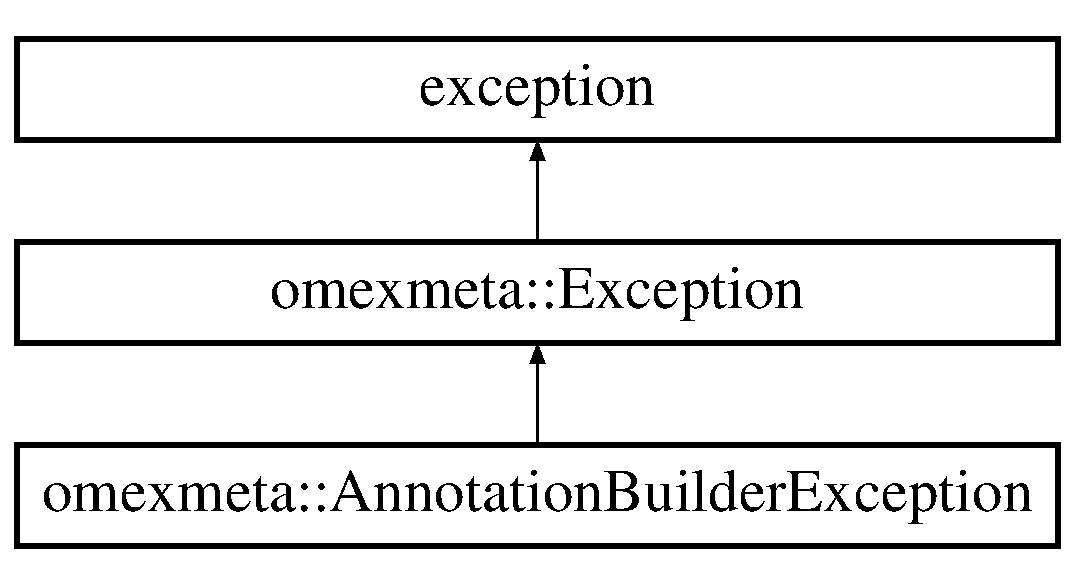
\includegraphics[height=3.000000cm]{classomexmeta_1_1AnnotationBuilderException}
\end{center}
\end{figure}
\subsection*{Additional Inherited Members}


The documentation for this class was generated from the following file\+:\begin{DoxyCompactItemize}
\item 
src/omexmeta/Error.\+h\end{DoxyCompactItemize}

\hypertarget{classomexmeta_1_1BiomodelsBiologyQualifier}{}\section{omexmeta\+:\+:Biomodels\+Biology\+Qualifier Class Reference}
\label{classomexmeta_1_1BiomodelsBiologyQualifier}\index{omexmeta\+::\+Biomodels\+Biology\+Qualifier@{omexmeta\+::\+Biomodels\+Biology\+Qualifier}}
Inheritance diagram for omexmeta\+:\+:Biomodels\+Biology\+Qualifier\+:\begin{figure}[H]
\begin{center}
\leavevmode
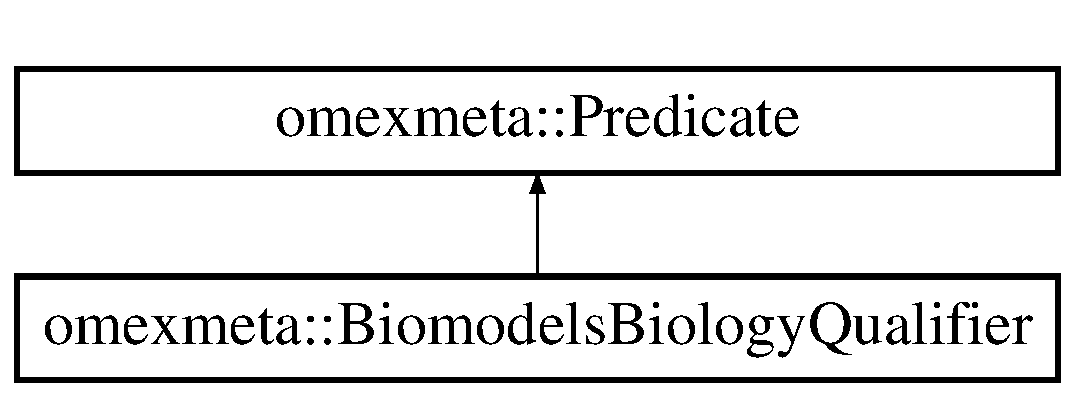
\includegraphics[height=2.000000cm]{classomexmeta_1_1BiomodelsBiologyQualifier}
\end{center}
\end{figure}
\subsection*{Public Member Functions}
\begin{DoxyCompactItemize}
\item 
\mbox{\Hypertarget{classomexmeta_1_1BiomodelsBiologyQualifier_a4dfa8fd975ceba60da6d3ccabdfb4514}\label{classomexmeta_1_1BiomodelsBiologyQualifier_a4dfa8fd975ceba60da6d3ccabdfb4514}} 
{\bfseries Biomodels\+Biology\+Qualifier} (const std\+::string \&term)
\item 
\mbox{\Hypertarget{classomexmeta_1_1BiomodelsBiologyQualifier_ade9766c18afa895e7c745aa4679ccfce}\label{classomexmeta_1_1BiomodelsBiologyQualifier_ade9766c18afa895e7c745aa4679ccfce}} 
void {\bfseries verify} ()
\end{DoxyCompactItemize}
\subsection*{Public Attributes}
\begin{DoxyCompactItemize}
\item 
std\+::vector$<$ std\+::string $>$ {\bfseries valid\+\_\+terms\+\_\+}
\end{DoxyCompactItemize}
\subsection*{Additional Inherited Members}


\subsection{Member Data Documentation}
\mbox{\Hypertarget{classomexmeta_1_1BiomodelsBiologyQualifier_a5ae1a3da58f05beb1e8b389f36f486bf}\label{classomexmeta_1_1BiomodelsBiologyQualifier_a5ae1a3da58f05beb1e8b389f36f486bf}} 
\index{omexmeta\+::\+Biomodels\+Biology\+Qualifier@{omexmeta\+::\+Biomodels\+Biology\+Qualifier}!valid\+\_\+terms\+\_\+@{valid\+\_\+terms\+\_\+}}
\index{valid\+\_\+terms\+\_\+@{valid\+\_\+terms\+\_\+}!omexmeta\+::\+Biomodels\+Biology\+Qualifier@{omexmeta\+::\+Biomodels\+Biology\+Qualifier}}
\subsubsection{\texorpdfstring{valid\+\_\+terms\+\_\+}{valid\_terms\_}}
{\footnotesize\ttfamily std\+::vector$<$std\+::string$>$ omexmeta\+::\+Biomodels\+Biology\+Qualifier\+::valid\+\_\+terms\+\_\+}

{\bfseries Initial value\+:}
\begin{DoxyCode}
\{
                \textcolor{stringliteral}{"is"},
                \textcolor{stringliteral}{"hasPart"},
                \textcolor{stringliteral}{"isPartOf"},
                \textcolor{stringliteral}{"isVersionOf"},
                \textcolor{stringliteral}{"hasVersion"},
                \textcolor{stringliteral}{"isHomologTo"},
                \textcolor{stringliteral}{"isDescribedBy"},
                \textcolor{stringliteral}{"isEncodedBy"},
                \textcolor{stringliteral}{"encodes"},
                \textcolor{stringliteral}{"occursIn"},
                \textcolor{stringliteral}{"hasProperty"},
                \textcolor{stringliteral}{"isPropertyOf"},
                \textcolor{stringliteral}{"hasTaxon"}
        \}
\end{DoxyCode}


The documentation for this class was generated from the following files\+:\begin{DoxyCompactItemize}
\item 
src/omexmeta/Predicate.\+h\item 
src/omexmeta/Predicate.\+cpp\end{DoxyCompactItemize}

\hypertarget{classomexmeta_1_1BiomodelsModelQualifier}{}\section{omexmeta\+:\+:Biomodels\+Model\+Qualifier Class Reference}
\label{classomexmeta_1_1BiomodelsModelQualifier}\index{omexmeta\+::\+Biomodels\+Model\+Qualifier@{omexmeta\+::\+Biomodels\+Model\+Qualifier}}
Inheritance diagram for omexmeta\+:\+:Biomodels\+Model\+Qualifier\+:\begin{figure}[H]
\begin{center}
\leavevmode
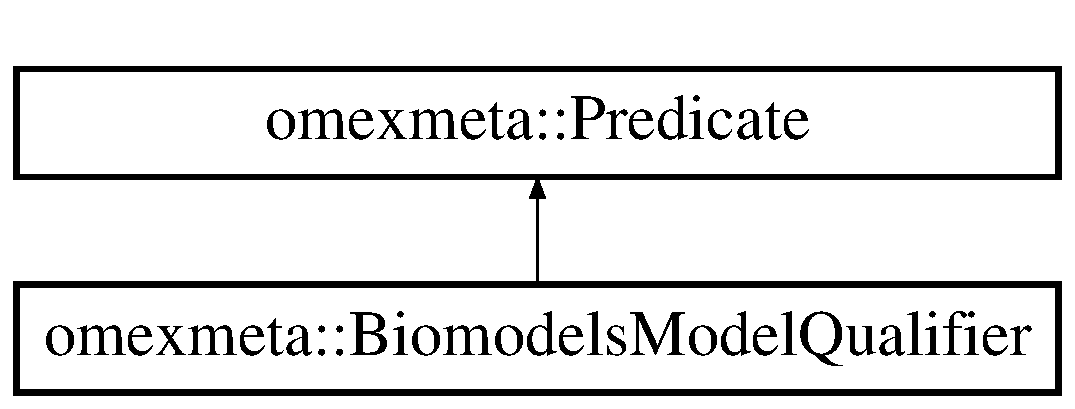
\includegraphics[height=2.000000cm]{classomexmeta_1_1BiomodelsModelQualifier}
\end{center}
\end{figure}
\subsection*{Public Member Functions}
\begin{DoxyCompactItemize}
\item 
\mbox{\Hypertarget{classomexmeta_1_1BiomodelsModelQualifier_a9842d4d8aa136cf4d617a53e12dc6f82}\label{classomexmeta_1_1BiomodelsModelQualifier_a9842d4d8aa136cf4d617a53e12dc6f82}} 
{\bfseries Biomodels\+Model\+Qualifier} (const std\+::string \&term)
\item 
\mbox{\Hypertarget{classomexmeta_1_1BiomodelsModelQualifier_a3d55d1629ea82f6bb20068818b462fee}\label{classomexmeta_1_1BiomodelsModelQualifier_a3d55d1629ea82f6bb20068818b462fee}} 
void {\bfseries verify} ()
\end{DoxyCompactItemize}
\subsection*{Public Attributes}
\begin{DoxyCompactItemize}
\item 
std\+::vector$<$ std\+::string $>$ {\bfseries valid\+\_\+terms\+\_\+}
\end{DoxyCompactItemize}
\subsection*{Additional Inherited Members}


\subsection{Member Data Documentation}
\mbox{\Hypertarget{classomexmeta_1_1BiomodelsModelQualifier_ab1d28ff2e7904f06b393a874f3d9607f}\label{classomexmeta_1_1BiomodelsModelQualifier_ab1d28ff2e7904f06b393a874f3d9607f}} 
\index{omexmeta\+::\+Biomodels\+Model\+Qualifier@{omexmeta\+::\+Biomodels\+Model\+Qualifier}!valid\+\_\+terms\+\_\+@{valid\+\_\+terms\+\_\+}}
\index{valid\+\_\+terms\+\_\+@{valid\+\_\+terms\+\_\+}!omexmeta\+::\+Biomodels\+Model\+Qualifier@{omexmeta\+::\+Biomodels\+Model\+Qualifier}}
\subsubsection{\texorpdfstring{valid\+\_\+terms\+\_\+}{valid\_terms\_}}
{\footnotesize\ttfamily std\+::vector$<$std\+::string$>$ omexmeta\+::\+Biomodels\+Model\+Qualifier\+::valid\+\_\+terms\+\_\+}

{\bfseries Initial value\+:}
\begin{DoxyCode}
\{
                \textcolor{stringliteral}{"isDerivedFrom"},
                \textcolor{stringliteral}{"isDescribedBy"},
                \textcolor{stringliteral}{"isInstanceOf"},
                \textcolor{stringliteral}{"hasInstance"},
        \}
\end{DoxyCode}


The documentation for this class was generated from the following files\+:\begin{DoxyCompactItemize}
\item 
src/omexmeta/Predicate.\+h\item 
src/omexmeta/Predicate.\+cpp\end{DoxyCompactItemize}

\hypertarget{classomexmeta_1_1CellMLAssistant}{}\section{omexmeta\+:\+:Cell\+M\+L\+Assistant Class Reference}
\label{classomexmeta_1_1CellMLAssistant}\index{omexmeta\+::\+Cell\+M\+L\+Assistant@{omexmeta\+::\+Cell\+M\+L\+Assistant}}
Inheritance diagram for omexmeta\+:\+:Cell\+M\+L\+Assistant\+:\begin{figure}[H]
\begin{center}
\leavevmode
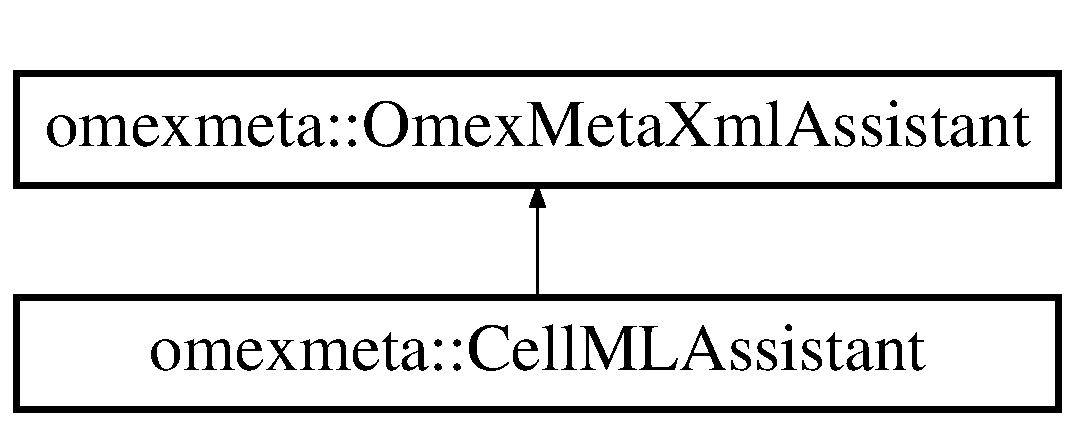
\includegraphics[height=2.000000cm]{classomexmeta_1_1CellMLAssistant}
\end{center}
\end{figure}
\subsection*{Public Member Functions}
\begin{DoxyCompactItemize}
\item 
\mbox{\Hypertarget{classomexmeta_1_1CellMLAssistant_ad0fa4e23c94197d5682a0f8e1dec0889}\label{classomexmeta_1_1CellMLAssistant_ad0fa4e23c94197d5682a0f8e1dec0889}} 
std\+::vector$<$ std\+::string $>$ {\bfseries get\+Valid\+Elements} () const override
\item 
\mbox{\Hypertarget{classomexmeta_1_1CellMLAssistant_a4aaccf21ed47201abaf20d67ad7bfaab}\label{classomexmeta_1_1CellMLAssistant_a4aaccf21ed47201abaf20d67ad7bfaab}} 
std\+::string {\bfseries meta\+Id\+Tag\+Name} () const override
\end{DoxyCompactItemize}


The documentation for this class was generated from the following files\+:\begin{DoxyCompactItemize}
\item 
src/omexmeta/Omex\+Meta\+Xml\+Assistant.\+h\item 
src/omexmeta/Omex\+Meta\+Xml\+Assistant.\+cpp\end{DoxyCompactItemize}

\hypertarget{classomexmeta_1_1CurlGet}{}\section{omexmeta\+:\+:Curl\+Get Class Reference}
\label{classomexmeta_1_1CurlGet}\index{omexmeta\+::\+Curl\+Get@{omexmeta\+::\+Curl\+Get}}
\subsection*{Static Public Member Functions}
\begin{DoxyCompactItemize}
\item 
\mbox{\Hypertarget{classomexmeta_1_1CurlGet_a52eaa2b1179cf49ec298022011b2477c}\label{classomexmeta_1_1CurlGet_a52eaa2b1179cf49ec298022011b2477c}} 
static int {\bfseries download} (const std\+::string \&url, const std\+::string \&output\+\_\+filename)
\end{DoxyCompactItemize}


The documentation for this class was generated from the following files\+:\begin{DoxyCompactItemize}
\item 
src/omexmeta/Curl\+Get.\+h\item 
src/omexmeta/Curl\+Get.\+cpp\end{DoxyCompactItemize}

\hypertarget{classomexmeta_1_1DCTerm}{}\section{omexmeta\+:\+:D\+C\+Term Class Reference}
\label{classomexmeta_1_1DCTerm}\index{omexmeta\+::\+D\+C\+Term@{omexmeta\+::\+D\+C\+Term}}
Inheritance diagram for omexmeta\+:\+:D\+C\+Term\+:\begin{figure}[H]
\begin{center}
\leavevmode
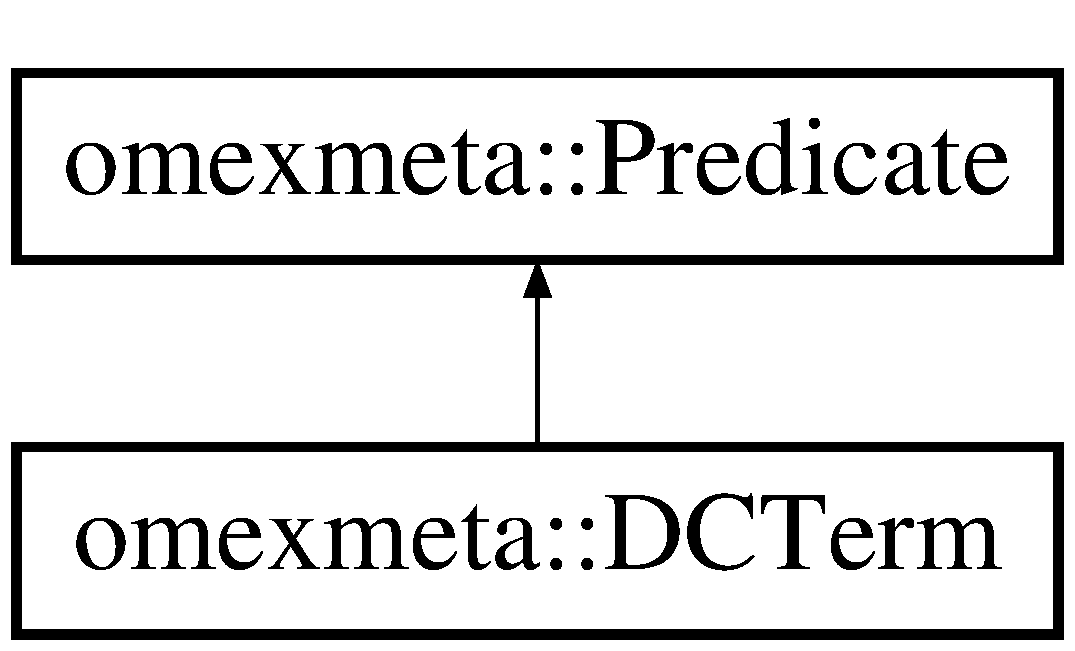
\includegraphics[height=2.000000cm]{classomexmeta_1_1DCTerm}
\end{center}
\end{figure}
\subsection*{Public Member Functions}
\begin{DoxyCompactItemize}
\item 
\mbox{\Hypertarget{classomexmeta_1_1DCTerm_a114081e0845c3f4c306b881da2d065cd}\label{classomexmeta_1_1DCTerm_a114081e0845c3f4c306b881da2d065cd}} 
{\bfseries D\+C\+Term} (const std\+::string \&term)
\item 
\mbox{\Hypertarget{classomexmeta_1_1DCTerm_aae02242702d1bb360c0a1ebb4dae8126}\label{classomexmeta_1_1DCTerm_aae02242702d1bb360c0a1ebb4dae8126}} 
void {\bfseries verify} ()
\end{DoxyCompactItemize}
\subsection*{Public Attributes}
\begin{DoxyCompactItemize}
\item 
std\+::vector$<$ std\+::string $>$ {\bfseries valid\+\_\+terms\+\_\+}
\end{DoxyCompactItemize}
\subsection*{Additional Inherited Members}


\subsection{Member Data Documentation}
\mbox{\Hypertarget{classomexmeta_1_1DCTerm_a3216c98de5a311d5f824dc132fefc3e4}\label{classomexmeta_1_1DCTerm_a3216c98de5a311d5f824dc132fefc3e4}} 
\index{omexmeta\+::\+D\+C\+Term@{omexmeta\+::\+D\+C\+Term}!valid\+\_\+terms\+\_\+@{valid\+\_\+terms\+\_\+}}
\index{valid\+\_\+terms\+\_\+@{valid\+\_\+terms\+\_\+}!omexmeta\+::\+D\+C\+Term@{omexmeta\+::\+D\+C\+Term}}
\subsubsection{\texorpdfstring{valid\+\_\+terms\+\_\+}{valid\_terms\_}}
{\footnotesize\ttfamily std\+::vector$<$std\+::string$>$ omexmeta\+::\+D\+C\+Term\+::valid\+\_\+terms\+\_\+}

{\bfseries Initial value\+:}
\begin{DoxyCode}
\{
                \textcolor{stringliteral}{"abstract"}, \textcolor{stringliteral}{"accessRights"}, \textcolor{stringliteral}{"accrualMethod"}, \textcolor{stringliteral}{"accrualPeriodicity"}, \textcolor{stringliteral}{"accrualPolicy"}, \textcolor{stringliteral}{"
      alternative"},
                \textcolor{stringliteral}{"audience"}, \textcolor{stringliteral}{"available"}, \textcolor{stringliteral}{"bibliographicCitation"}, \textcolor{stringliteral}{"conformsTo"}, \textcolor{stringliteral}{"contributor"}, \textcolor{stringliteral}{"coverage"}, \textcolor{stringliteral}{
      "created"},
                \textcolor{stringliteral}{"creator"}, \textcolor{stringliteral}{"date"}, \textcolor{stringliteral}{"dateAccepted"}, \textcolor{stringliteral}{"dateCopyrighted"}, \textcolor{stringliteral}{"dateSubmitted"}, \textcolor{stringliteral}{"description"}, \textcolor{stringliteral}{"
      educationLevel"},
                \textcolor{stringliteral}{"extent"}, \textcolor{stringliteral}{"format"}, \textcolor{stringliteral}{"hasFormat"}, \textcolor{stringliteral}{"hasPart"}, \textcolor{stringliteral}{"hasVersion"}, \textcolor{stringliteral}{"identifier"}, \textcolor{stringliteral}{"
      instructionalMethod"},
                \textcolor{stringliteral}{"isFormatOf"}, \textcolor{stringliteral}{"isPartOf"}, \textcolor{stringliteral}{"isReferencedBy"}, \textcolor{stringliteral}{"isReplacedBy"}, \textcolor{stringliteral}{"isRequiredBy"}, \textcolor{stringliteral}{"issued"}, \textcolor{stringliteral}{"
      isVersionOf"},
                \textcolor{stringliteral}{"language"}, \textcolor{stringliteral}{"license"}, \textcolor{stringliteral}{"mediator"}, \textcolor{stringliteral}{"medium"}, \textcolor{stringliteral}{"modified"}, \textcolor{stringliteral}{"provenance"}, \textcolor{stringliteral}{"publisher"}, \textcolor{stringliteral}{"
      references"},
                \textcolor{stringliteral}{"relation"}, \textcolor{stringliteral}{"replaces"}, \textcolor{stringliteral}{"requires"}, \textcolor{stringliteral}{"rights"}, \textcolor{stringliteral}{"rightsHolder"}, \textcolor{stringliteral}{"source"}, \textcolor{stringliteral}{"spatial"}, \textcolor{stringliteral}{"subject
      "},
                \textcolor{stringliteral}{"tableOfContents"}, \textcolor{stringliteral}{"temporal"}, \textcolor{stringliteral}{"title"}, \textcolor{stringliteral}{"type"}, \textcolor{stringliteral}{"valid"},\}
\end{DoxyCode}


The documentation for this class was generated from the following files\+:\begin{DoxyCompactItemize}
\item 
src/omexmeta/Predicate.\+h\item 
src/omexmeta/Predicate.\+cpp\end{DoxyCompactItemize}

\hypertarget{classdbg_1_1DebugOutput}{}\section{dbg\+:\+:Debug\+Output Class Reference}
\label{classdbg_1_1DebugOutput}\index{dbg\+::\+Debug\+Output@{dbg\+::\+Debug\+Output}}
\subsection*{Public Types}
\begin{DoxyCompactItemize}
\item 
\mbox{\Hypertarget{classdbg_1_1DebugOutput_a5d9b38d5b9276cb584c0e20e9b1a2045}\label{classdbg_1_1DebugOutput_a5d9b38d5b9276cb584c0e20e9b1a2045}} 
using {\bfseries expr\+\_\+t} = const char $\ast$
\end{DoxyCompactItemize}
\subsection*{Public Member Functions}
\begin{DoxyCompactItemize}
\item 
\mbox{\Hypertarget{classdbg_1_1DebugOutput_a7bb0378758aa1006e2423eff57ee36a2}\label{classdbg_1_1DebugOutput_a7bb0378758aa1006e2423eff57ee36a2}} 
{\bfseries Debug\+Output} (const char $\ast$filepath, int line, const char $\ast$function\+\_\+name)
\item 
\mbox{\Hypertarget{classdbg_1_1DebugOutput_aa135787802db4a6b0b4eb185185e13ca}\label{classdbg_1_1DebugOutput_aa135787802db4a6b0b4eb185185e13ca}} 
{\footnotesize template$<$typename... T$>$ }\\auto {\bfseries print} (std\+::initializer\+\_\+list$<$ expr\+\_\+t $>$ exprs, std\+::initializer\+\_\+list$<$ std\+::string $>$ types, T \&\&... values) -\/$>$ last\+\_\+t$<$ T... $>$
\end{DoxyCompactItemize}


The documentation for this class was generated from the following file\+:\begin{DoxyCompactItemize}
\item 
src/omexmeta/dbg.\+h\end{DoxyCompactItemize}

\hypertarget{structdbg_1_1detail__detector_1_1detector}{}\section{dbg\+:\+:detail\+\_\+detector\+:\+:detector$<$ Default, Always\+Void, Op, Args $>$ Struct Template Reference}
\label{structdbg_1_1detail__detector_1_1detector}\index{dbg\+::detail\+\_\+detector\+::detector$<$ Default, Always\+Void, Op, Args $>$@{dbg\+::detail\+\_\+detector\+::detector$<$ Default, Always\+Void, Op, Args $>$}}
\subsection*{Public Types}
\begin{DoxyCompactItemize}
\item 
\mbox{\Hypertarget{structdbg_1_1detail__detector_1_1detector_af1b6da4282d723669e926c52f446a989}\label{structdbg_1_1detail__detector_1_1detector_af1b6da4282d723669e926c52f446a989}} 
using {\bfseries value\+\_\+t} = std\+::false\+\_\+type
\item 
\mbox{\Hypertarget{structdbg_1_1detail__detector_1_1detector_aab6b446944545683b9533ea8fc623480}\label{structdbg_1_1detail__detector_1_1detector_aab6b446944545683b9533ea8fc623480}} 
using {\bfseries type} = Default
\end{DoxyCompactItemize}


The documentation for this struct was generated from the following file\+:\begin{DoxyCompactItemize}
\item 
src/omexmeta/dbg.\+h\end{DoxyCompactItemize}

\hypertarget{structdbg_1_1detail__detector_1_1detector_3_01Default_00_01void__t_3_01Op_3_01Args_8_8_8_01_4_01_4_00_01Op_00_01Args_8_8_8_01_4}{}\section{dbg\+:\+:detail\+\_\+detector\+:\+:detector$<$ Default, void\+\_\+t$<$ Op$<$ Args... $>$ $>$, Op, Args... $>$ Struct Template Reference}
\label{structdbg_1_1detail__detector_1_1detector_3_01Default_00_01void__t_3_01Op_3_01Args_8_8_8_01_4_01_4_00_01Op_00_01Args_8_8_8_01_4}\index{dbg\+::detail\+\_\+detector\+::detector$<$ Default, void\+\_\+t$<$ Op$<$ Args... $>$ $>$, Op, Args... $>$@{dbg\+::detail\+\_\+detector\+::detector$<$ Default, void\+\_\+t$<$ Op$<$ Args... $>$ $>$, Op, Args... $>$}}
\subsection*{Public Types}
\begin{DoxyCompactItemize}
\item 
\mbox{\Hypertarget{structdbg_1_1detail__detector_1_1detector_3_01Default_00_01void__t_3_01Op_3_01Args_8_8_8_01_4_01_4_00_01Op_00_01Args_8_8_8_01_4_ab9dc20c0565be267d2d98b0e0f4a565b}\label{structdbg_1_1detail__detector_1_1detector_3_01Default_00_01void__t_3_01Op_3_01Args_8_8_8_01_4_01_4_00_01Op_00_01Args_8_8_8_01_4_ab9dc20c0565be267d2d98b0e0f4a565b}} 
using {\bfseries value\+\_\+t} = std\+::true\+\_\+type
\item 
\mbox{\Hypertarget{structdbg_1_1detail__detector_1_1detector_3_01Default_00_01void__t_3_01Op_3_01Args_8_8_8_01_4_01_4_00_01Op_00_01Args_8_8_8_01_4_a2119ba35e684b8292286546a1cea10d1}\label{structdbg_1_1detail__detector_1_1detector_3_01Default_00_01void__t_3_01Op_3_01Args_8_8_8_01_4_01_4_00_01Op_00_01Args_8_8_8_01_4_a2119ba35e684b8292286546a1cea10d1}} 
using {\bfseries type} = Op$<$ Args... $>$
\end{DoxyCompactItemize}


The documentation for this struct was generated from the following file\+:\begin{DoxyCompactItemize}
\item 
src/omexmeta/dbg.\+h\end{DoxyCompactItemize}

\hypertarget{classomexmeta_1_1Editor}{}\section{omexmeta\+:\+:Editor Class Reference}
\label{classomexmeta_1_1Editor}\index{omexmeta\+::\+Editor@{omexmeta\+::\+Editor}}
\subsection*{Public Member Functions}
\begin{DoxyCompactItemize}
\item 
\mbox{\Hypertarget{classomexmeta_1_1Editor_a6ac976c1a3762f77a577b5735cd509f4}\label{classomexmeta_1_1Editor_a6ac976c1a3762f77a577b5735cd509f4}} 
{\bfseries Editor} (const std\+::string \&xml, bool create\+\_\+ids, const \hyperlink{classredland_1_1LibrdfModel}{Librdf\+Model} \&model, Namespace\+Map \&ns\+\_\+map, bool generate\+\_\+new\+\_\+metaids=false, bool sbml\+\_\+semantic\+\_\+extraction=true, const std\+::string \&repository\+\_\+uri=std\+::string(), const std\+::string \&archive\+\_\+uri=std\+::string(), const std\+::string \&model\+\_\+uri=std\+::string(), const std\+::string \&local\+\_\+uri=std\+::string())
\item 
\mbox{\Hypertarget{classomexmeta_1_1Editor_ab5b39f1f137312ce77575e73a86dfb05}\label{classomexmeta_1_1Editor_ab5b39f1f137312ce77575e73a86dfb05}} 
int {\bfseries size} () const
\item 
\mbox{\Hypertarget{classomexmeta_1_1Editor_a514443fe99a6e52154d1fe4f7ec94618}\label{classomexmeta_1_1Editor_a514443fe99a6e52154d1fe4f7ec94618}} 
const Namespace\+Map \& {\bfseries get\+Namespaces} () const
\item 
\mbox{\Hypertarget{classomexmeta_1_1Editor_a4b2610fb802eb306349d69ae6fde60c0}\label{classomexmeta_1_1Editor_a4b2610fb802eb306349d69ae6fde60c0}} 
librdf\+\_\+model $\ast$ {\bfseries get\+Model} () const
\item 
\mbox{\Hypertarget{classomexmeta_1_1Editor_a83836e19bb1de9c7df69d36e8b61b2b2}\label{classomexmeta_1_1Editor_a83836e19bb1de9c7df69d36e8b61b2b2}} 
void {\bfseries set\+Namespaces} (const Namespace\+Map \&namespaces)
\item 
\mbox{\Hypertarget{classomexmeta_1_1Editor_ad931e829fc9f78717e0c1443c619b7d3}\label{classomexmeta_1_1Editor_ad931e829fc9f78717e0c1443c619b7d3}} 
const std\+::string \& {\bfseries get\+Xml} () const
\item 
\mbox{\Hypertarget{classomexmeta_1_1Editor_a242c86222e1aeff337d3af22641db1de}\label{classomexmeta_1_1Editor_a242c86222e1aeff337d3af22641db1de}} 
const std\+::vector$<$ std\+::string $>$ \& {\bfseries get\+Metaids} () const
\item 
\mbox{\Hypertarget{classomexmeta_1_1Editor_a052a725cee8b8e577c55e977eee81ace}\label{classomexmeta_1_1Editor_a052a725cee8b8e577c55e977eee81ace}} 
void {\bfseries add\+Namespace} (const std\+::string \&ns, std\+::string prefix)
\item 
\mbox{\Hypertarget{classomexmeta_1_1Editor_a0417b55575a244817ef981f17c8e1a8f}\label{classomexmeta_1_1Editor_a0417b55575a244817ef981f17c8e1a8f}} 
void {\bfseries add\+Single\+Annotation} (\hyperlink{classomexmeta_1_1Subject}{Subject} subject, const Predicate\+Ptr \&predicate\+\_\+ptr, const \hyperlink{classomexmeta_1_1Resource}{Resource} \&resource)
\item 
\mbox{\Hypertarget{classomexmeta_1_1Editor_ae46835f3f35425d8087b80d08666aaa4}\label{classomexmeta_1_1Editor_ae46835f3f35425d8087b80d08666aaa4}} 
void {\bfseries add\+Single\+Annotation} (\hyperlink{classomexmeta_1_1Triple}{Singular\+Annotation} \&singular\+Annotation)
\item 
\mbox{\Hypertarget{classomexmeta_1_1Editor_afcb5ce7397aab23fabd3b4b4b89d3a54}\label{classomexmeta_1_1Editor_afcb5ce7397aab23fabd3b4b4b89d3a54}} 
void {\bfseries remove\+Single\+Annotation} (const \hyperlink{classomexmeta_1_1Triple}{Singular\+Annotation} \&singular\+Annotation) const
\item 
\mbox{\Hypertarget{classomexmeta_1_1Editor_a146ae84fb44991d9c6135e98f03fa972}\label{classomexmeta_1_1Editor_a146ae84fb44991d9c6135e98f03fa972}} 
void {\bfseries add\+Composite\+Annotation} (\hyperlink{classomexmeta_1_1PhysicalPhenomenon}{Physical\+Phenomenon} $\ast$phenomenon\+Ptr)
\item 
\mbox{\Hypertarget{classomexmeta_1_1Editor_a0740831baafe244374ad7a324d51a87e}\label{classomexmeta_1_1Editor_a0740831baafe244374ad7a324d51a87e}} 
void {\bfseries add\+Physical\+Entity} (\hyperlink{classomexmeta_1_1PhysicalEntity}{Physical\+Entity} \&physical\+Entity)
\item 
\mbox{\Hypertarget{classomexmeta_1_1Editor_a0acf94314252b70a4db89f83e6047e8f}\label{classomexmeta_1_1Editor_a0acf94314252b70a4db89f83e6047e8f}} 
void {\bfseries remove\+Physical\+Entity} (\hyperlink{classomexmeta_1_1PhysicalEntity}{Physical\+Entity} \&physical\+Entity) const
\item 
\mbox{\Hypertarget{classomexmeta_1_1Editor_a8be7fa01bef49ff1c93965781797c9bc}\label{classomexmeta_1_1Editor_a8be7fa01bef49ff1c93965781797c9bc}} 
void {\bfseries remove\+Personal\+Information} (\hyperlink{classomexmeta_1_1PersonalInformation}{Personal\+Information} $\ast$information) const
\item 
\mbox{\Hypertarget{classomexmeta_1_1Editor_ae4a608ecbe64f05c1b64efbeeb1fdeb1}\label{classomexmeta_1_1Editor_ae4a608ecbe64f05c1b64efbeeb1fdeb1}} 
void {\bfseries add\+Physical\+Process} (\hyperlink{classomexmeta_1_1PhysicalProcess}{Physical\+Process} \&physical\+Process)
\item 
\mbox{\Hypertarget{classomexmeta_1_1Editor_a42640d74c6afe780738c906bdf346a78}\label{classomexmeta_1_1Editor_a42640d74c6afe780738c906bdf346a78}} 
void {\bfseries remove\+Physical\+Process} (\hyperlink{classomexmeta_1_1PhysicalProcess}{Physical\+Process} \&physical\+Process) const
\item 
\mbox{\Hypertarget{classomexmeta_1_1Editor_a7833e03995f6323109c2db8d59104f6c}\label{classomexmeta_1_1Editor_a7833e03995f6323109c2db8d59104f6c}} 
void {\bfseries add\+Physical\+Force} (\hyperlink{classomexmeta_1_1PhysicalForce}{Physical\+Force} \&physical\+Force)
\item 
\mbox{\Hypertarget{classomexmeta_1_1Editor_a1b2e0f5859fe2e2784ecff2a78f7f1f8}\label{classomexmeta_1_1Editor_a1b2e0f5859fe2e2784ecff2a78f7f1f8}} 
void {\bfseries add\+Personal\+Information} (\hyperlink{classomexmeta_1_1PersonalInformation}{Personal\+Information} $\ast$personal\+Information)
\item 
\mbox{\Hypertarget{classomexmeta_1_1Editor_ad99187ec52bef1af440af5d9560f32c5}\label{classomexmeta_1_1Editor_ad99187ec52bef1af440af5d9560f32c5}} 
void {\bfseries remove\+Physical\+Force} (\hyperlink{classomexmeta_1_1PhysicalForce}{Physical\+Force} \&physical\+Force) const
\item 
\mbox{\Hypertarget{classomexmeta_1_1Editor_a790458ef32f01ce0a6fd87bf14bed81a}\label{classomexmeta_1_1Editor_a790458ef32f01ce0a6fd87bf14bed81a}} 
void {\bfseries check\+Valid\+Metaid} (const std\+::string \&metaid)
\item 
\mbox{\Hypertarget{classomexmeta_1_1Editor_a3fef7f1c38949b50239a9a07cc327d67}\label{classomexmeta_1_1Editor_a3fef7f1c38949b50239a9a07cc327d67}} 
void {\bfseries add\+Namespace\+From\+Annotation} (const std\+::string \&predicate\+\_\+string)
\item 
\mbox{\Hypertarget{classomexmeta_1_1Editor_af987e450e4bf9d75391ad3f5ac6233f6}\label{classomexmeta_1_1Editor_af987e450e4bf9d75391ad3f5ac6233f6}} 
const std\+::string \& {\bfseries get\+Metaid\+Base} () const
\item 
\mbox{\Hypertarget{classomexmeta_1_1Editor_a206feee18473abbeda5e4e55906e73eb}\label{classomexmeta_1_1Editor_a206feee18473abbeda5e4e55906e73eb}} 
void {\bfseries set\+Metaid\+Base} (const std\+::string \&metaid\+Base)
\item 
\mbox{\Hypertarget{classomexmeta_1_1Editor_a68ade6a293061a98243a3b2853e55a4b}\label{classomexmeta_1_1Editor_a68ade6a293061a98243a3b2853e55a4b}} 
Omex\+Meta\+Xml\+Type {\bfseries get\+Type} () const
\item 
\mbox{\Hypertarget{classomexmeta_1_1Editor_a3e2c493ed5034a15e6915b7b649b58a3}\label{classomexmeta_1_1Editor_a3e2c493ed5034a15e6915b7b649b58a3}} 
void {\bfseries set\+Type} (Omex\+Meta\+Xml\+Type type)
\item 
\mbox{\Hypertarget{classomexmeta_1_1Editor_a245b2105c175892d1fddaf693fa9d636}\label{classomexmeta_1_1Editor_a245b2105c175892d1fddaf693fa9d636}} 
\hyperlink{classomexmeta_1_1PhysicalEntity}{Physical\+Entity} {\bfseries new\+Physical\+Entity} ()
\item 
\mbox{\Hypertarget{classomexmeta_1_1Editor_a58d21ef09f3dc5a6a66dbafe34150695}\label{classomexmeta_1_1Editor_a58d21ef09f3dc5a6a66dbafe34150695}} 
\hyperlink{classomexmeta_1_1PhysicalForce}{Physical\+Force} {\bfseries new\+Physical\+Force} ()
\item 
\mbox{\Hypertarget{classomexmeta_1_1Editor_a2815d918736ee17d07306c5cf07c8ebf}\label{classomexmeta_1_1Editor_a2815d918736ee17d07306c5cf07c8ebf}} 
\hyperlink{classomexmeta_1_1PhysicalProcess}{Physical\+Process} {\bfseries new\+Physical\+Process} ()
\item 
\mbox{\Hypertarget{classomexmeta_1_1Editor_a1943079ddbc4a4c6d896f51f360a11df}\label{classomexmeta_1_1Editor_a1943079ddbc4a4c6d896f51f360a11df}} 
\hyperlink{classomexmeta_1_1PersonalInformation}{Personal\+Information} {\bfseries new\+Personal\+Information} ()
\item 
\mbox{\Hypertarget{classomexmeta_1_1Editor_a8fb3a19e8f64aeff2ac9b78c483843de}\label{classomexmeta_1_1Editor_a8fb3a19e8f64aeff2ac9b78c483843de}} 
void {\bfseries add\+Single\+Annotation\+No\+Validation} (\hyperlink{classomexmeta_1_1Triple}{Singular\+Annotation} \&singular\+Annotation)
\item 
\mbox{\Hypertarget{classomexmeta_1_1Editor_ad05d04a31263f9c7cb8105e29fd9d158}\label{classomexmeta_1_1Editor_ad05d04a31263f9c7cb8105e29fd9d158}} 
void {\bfseries add\+Composite\+Annotation2} (\hyperlink{classomexmeta_1_1PhysicalPhenomenon}{Physical\+Phenomenon} $\ast$phenomenon\+Ptr)
\item 
\mbox{\Hypertarget{classomexmeta_1_1Editor_ace8ee873498fa72b63c0747775b729f5}\label{classomexmeta_1_1Editor_ace8ee873498fa72b63c0747775b729f5}} 
void {\bfseries add\+Triples} (\hyperlink{classomexmeta_1_1Triples}{Triples} \&triples)
\item 
\mbox{\Hypertarget{classomexmeta_1_1Editor_af00f00108238acbf2b2974cedc07b454}\label{classomexmeta_1_1Editor_af00f00108238acbf2b2974cedc07b454}} 
void {\bfseries remove\+Physical\+Phenomenon} (\hyperlink{classomexmeta_1_1PhysicalPhenomenon}{Physical\+Phenomenon} $\ast$physical\+Phenomenon) const
\item 
\mbox{\Hypertarget{classomexmeta_1_1Editor_a736e49794c5a358f06d13d41c3657fe2}\label{classomexmeta_1_1Editor_a736e49794c5a358f06d13d41c3657fe2}} 
std\+::string {\bfseries get\+Archive\+Uri} () const
\item 
\mbox{\Hypertarget{classomexmeta_1_1Editor_a8494826923de713c19f971fd9c7908c0}\label{classomexmeta_1_1Editor_a8494826923de713c19f971fd9c7908c0}} 
std\+::string {\bfseries get\+Local\+Uri} () const
\item 
\mbox{\Hypertarget{classomexmeta_1_1Editor_a0020d3b9c3e91fb37c134ba8b211c13e}\label{classomexmeta_1_1Editor_a0020d3b9c3e91fb37c134ba8b211c13e}} 
std\+::string {\bfseries get\+Model\+Uri} () const
\item 
\mbox{\Hypertarget{classomexmeta_1_1Editor_a2264cbd2efae17d1d72c3f402d8721bf}\label{classomexmeta_1_1Editor_a2264cbd2efae17d1d72c3f402d8721bf}} 
std\+::string {\bfseries get\+Repository\+Uri} () const
\item 
\mbox{\Hypertarget{classomexmeta_1_1Editor_a5143e1f8db82393faed322810acf5e92}\label{classomexmeta_1_1Editor_a5143e1f8db82393faed322810acf5e92}} 
\hyperlink{classredland_1_1LibrdfNode}{Librdf\+Node} {\bfseries create\+Node\+With\+Model\+Uri} (const std\+::string \&string) const
\item 
\mbox{\Hypertarget{classomexmeta_1_1Editor_a9c8b060005146f3cf5a231ea6789e7d7}\label{classomexmeta_1_1Editor_a9c8b060005146f3cf5a231ea6789e7d7}} 
void {\bfseries add\+Creator} (std\+::string orcid\+\_\+id)
\item 
\mbox{\Hypertarget{classomexmeta_1_1Editor_a8b83488faf68546733114acf54595b02}\label{classomexmeta_1_1Editor_a8b83488faf68546733114acf54595b02}} 
void {\bfseries add\+Curator} (std\+::string orcid\+\_\+id)
\item 
\mbox{\Hypertarget{classomexmeta_1_1Editor_af64f0cac6b7e27b121df94ab5b1fa217}\label{classomexmeta_1_1Editor_af64f0cac6b7e27b121df94ab5b1fa217}} 
void {\bfseries add\+Taxon} (const std\+::string \&taxon\+\_\+id)
\item 
\mbox{\Hypertarget{classomexmeta_1_1Editor_a533f93c8ae0c3081dfe2fc8e8ebee8ea}\label{classomexmeta_1_1Editor_a533f93c8ae0c3081dfe2fc8e8ebee8ea}} 
void {\bfseries add\+Pubmed} (const std\+::string \&pubmedid)
\item 
\mbox{\Hypertarget{classomexmeta_1_1Editor_a8526a87544b1265695f1749100da5fa2}\label{classomexmeta_1_1Editor_a8526a87544b1265695f1749100da5fa2}} 
void {\bfseries add\+Description} (const std\+::string \&date)
\item 
\mbox{\Hypertarget{classomexmeta_1_1Editor_ae1b146f142ec10237f8edbecf0368f8e}\label{classomexmeta_1_1Editor_ae1b146f142ec10237f8edbecf0368f8e}} 
void {\bfseries add\+Date\+Created} (const std\+::string \&date)
\item 
\mbox{\Hypertarget{classomexmeta_1_1Editor_a50674b2591d2fed572954ac8490ee21c}\label{classomexmeta_1_1Editor_a50674b2591d2fed572954ac8490ee21c}} 
\hyperlink{classomexmeta_1_1Triple}{Singular\+Annotation} {\bfseries new\+Singular\+Annotation} (std\+::string metaid) const
\item 
\mbox{\Hypertarget{classomexmeta_1_1Editor_ad7240613a1f3e215af6e4a05d121508c}\label{classomexmeta_1_1Editor_ad7240613a1f3e215af6e4a05d121508c}} 
void {\bfseries add\+Parent\+Model} (const std\+::string \&biomod\+\_\+id)
\item 
\mbox{\Hypertarget{classomexmeta_1_1Editor_ae97ebb9bb2bc3ebd7d3b0a5eca9dfb0f}\label{classomexmeta_1_1Editor_ae97ebb9bb2bc3ebd7d3b0a5eca9dfb0f}} 
void {\bfseries add\+Personal\+Information} (\hyperlink{classomexmeta_1_1PersonalInformation}{Personal\+Information} $\ast$personal\+Information) const
\item 
\mbox{\Hypertarget{classomexmeta_1_1Editor_a6142da2b89068e9638410c3c903e3b64}\label{classomexmeta_1_1Editor_a6142da2b89068e9638410c3c903e3b64}} 
\hyperlink{classomexmeta_1_1Triple}{Singular\+Annotation} {\bfseries new\+Singular\+Annotation} () const
\end{DoxyCompactItemize}


The documentation for this class was generated from the following files\+:\begin{DoxyCompactItemize}
\item 
src/omexmeta/Editor.\+h\item 
src/omexmeta/Editor.\+cpp\end{DoxyCompactItemize}

\hypertarget{classomexmeta_1_1ElementExtractor}{}\section{omexmeta\+:\+:Element\+Extractor Class Reference}
\label{classomexmeta_1_1ElementExtractor}\index{omexmeta\+::\+Element\+Extractor@{omexmeta\+::\+Element\+Extractor}}
\subsection*{Public Member Functions}
\begin{DoxyCompactItemize}
\item 
\mbox{\Hypertarget{classomexmeta_1_1ElementExtractor_a9de35d2d6cf78dad4fa9fb2f46fa8e37}\label{classomexmeta_1_1ElementExtractor_a9de35d2d6cf78dad4fa9fb2f46fa8e37}} 
{\bfseries Element\+Extractor} (const std\+::string \&markup, const std\+::string \&element)
\item 
\mbox{\Hypertarget{classomexmeta_1_1ElementExtractor_aedddcdb8149ac96e76f20ffd56980b0c}\label{classomexmeta_1_1ElementExtractor_aedddcdb8149ac96e76f20ffd56980b0c}} 
const std\+::vector$<$ xml\+Node $\ast$ $>$ \& {\bfseries get\+Elements} () const
\end{DoxyCompactItemize}


The documentation for this class was generated from the following files\+:\begin{DoxyCompactItemize}
\item 
src/omexmeta/Element\+Extractor.\+h\item 
src/omexmeta/Element\+Extractor.\+cpp\end{DoxyCompactItemize}

\hypertarget{classomexmeta_1_1Exception}{}\section{omexmeta\+:\+:Exception Class Reference}
\label{classomexmeta_1_1Exception}\index{omexmeta\+::\+Exception@{omexmeta\+::\+Exception}}


\href{https://stackoverflow.com/questions/8152720/correct-way-to-inherit-from-stdexception}{\tt https\+://stackoverflow.\+com/questions/8152720/correct-\/way-\/to-\/inherit-\/from-\/stdexception}  




{\ttfamily \#include $<$Error.\+h$>$}

Inheritance diagram for omexmeta\+:\+:Exception\+:\begin{figure}[H]
\begin{center}
\leavevmode
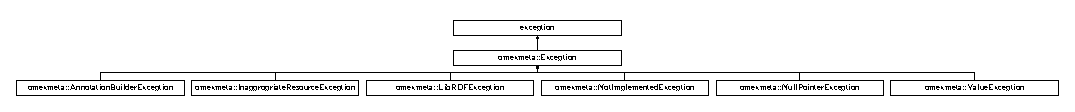
\includegraphics[height=1.056604cm]{classomexmeta_1_1Exception}
\end{center}
\end{figure}
\subsection*{Public Member Functions}
\begin{DoxyCompactItemize}
\item 
\hyperlink{classomexmeta_1_1Exception_ad09e2a190a245199974678e2790e81ff}{Exception} (const char $\ast$message)
\item 
\hyperlink{classomexmeta_1_1Exception_ac50b0a25504303cc1a4a1a20de0127eb}{Exception} (std\+::string message)
\item 
\hyperlink{classomexmeta_1_1Exception_aaa08b2467c40a3e28586c0da5da45736}{$\sim$\+Exception} () noexcept override=default
\item 
const char $\ast$ \hyperlink{classomexmeta_1_1Exception_af9c3f258e4715dd2102f5c2db5fbe260}{what} () const noexcept override
\end{DoxyCompactItemize}
\subsection*{Protected Attributes}
\begin{DoxyCompactItemize}
\item 
std\+::string \hyperlink{classomexmeta_1_1Exception_a99067aa4ed7e38cf27b986cca3734512}{msg\+\_\+}
\end{DoxyCompactItemize}


\subsection{Detailed Description}
\href{https://stackoverflow.com/questions/8152720/correct-way-to-inherit-from-stdexception}{\tt https\+://stackoverflow.\+com/questions/8152720/correct-\/way-\/to-\/inherit-\/from-\/stdexception} 

\subsection{Constructor \& Destructor Documentation}
\mbox{\Hypertarget{classomexmeta_1_1Exception_ad09e2a190a245199974678e2790e81ff}\label{classomexmeta_1_1Exception_ad09e2a190a245199974678e2790e81ff}} 
\index{omexmeta\+::\+Exception@{omexmeta\+::\+Exception}!Exception@{Exception}}
\index{Exception@{Exception}!omexmeta\+::\+Exception@{omexmeta\+::\+Exception}}
\subsubsection{\texorpdfstring{Exception()}{Exception()}\hspace{0.1cm}{\footnotesize\ttfamily [1/2]}}
{\footnotesize\ttfamily omexmeta\+::\+Exception\+::\+Exception (\begin{DoxyParamCaption}\item[{const char $\ast$}]{message }\end{DoxyParamCaption})\hspace{0.3cm}{\ttfamily [inline]}, {\ttfamily [explicit]}}

Constructor (C strings). 
\begin{DoxyParams}{Parameters}
{\em message} & C-\/style string error message. The string contents are copied upon construction. Hence, responsibility for deleting the char$\ast$ lies with the caller. \\
\hline
\end{DoxyParams}
\mbox{\Hypertarget{classomexmeta_1_1Exception_ac50b0a25504303cc1a4a1a20de0127eb}\label{classomexmeta_1_1Exception_ac50b0a25504303cc1a4a1a20de0127eb}} 
\index{omexmeta\+::\+Exception@{omexmeta\+::\+Exception}!Exception@{Exception}}
\index{Exception@{Exception}!omexmeta\+::\+Exception@{omexmeta\+::\+Exception}}
\subsubsection{\texorpdfstring{Exception()}{Exception()}\hspace{0.1cm}{\footnotesize\ttfamily [2/2]}}
{\footnotesize\ttfamily omexmeta\+::\+Exception\+::\+Exception (\begin{DoxyParamCaption}\item[{std\+::string}]{message }\end{DoxyParamCaption})\hspace{0.3cm}{\ttfamily [inline]}, {\ttfamily [explicit]}}

Constructor (C++ S\+TL strings). 
\begin{DoxyParams}{Parameters}
{\em message} & The error message. \\
\hline
\end{DoxyParams}
\mbox{\Hypertarget{classomexmeta_1_1Exception_aaa08b2467c40a3e28586c0da5da45736}\label{classomexmeta_1_1Exception_aaa08b2467c40a3e28586c0da5da45736}} 
\index{omexmeta\+::\+Exception@{omexmeta\+::\+Exception}!````~Exception@{$\sim$\+Exception}}
\index{````~Exception@{$\sim$\+Exception}!omexmeta\+::\+Exception@{omexmeta\+::\+Exception}}
\subsubsection{\texorpdfstring{$\sim$\+Exception()}{~Exception()}}
{\footnotesize\ttfamily omexmeta\+::\+Exception\+::$\sim$\+Exception (\begin{DoxyParamCaption}{ }\end{DoxyParamCaption})\hspace{0.3cm}{\ttfamily [override]}, {\ttfamily [default]}, {\ttfamily [noexcept]}}

Destructor. Virtual to allow for subclassing. 

\subsection{Member Function Documentation}
\mbox{\Hypertarget{classomexmeta_1_1Exception_af9c3f258e4715dd2102f5c2db5fbe260}\label{classomexmeta_1_1Exception_af9c3f258e4715dd2102f5c2db5fbe260}} 
\index{omexmeta\+::\+Exception@{omexmeta\+::\+Exception}!what@{what}}
\index{what@{what}!omexmeta\+::\+Exception@{omexmeta\+::\+Exception}}
\subsubsection{\texorpdfstring{what()}{what()}}
{\footnotesize\ttfamily const char$\ast$ omexmeta\+::\+Exception\+::what (\begin{DoxyParamCaption}{ }\end{DoxyParamCaption}) const\hspace{0.3cm}{\ttfamily [inline]}, {\ttfamily [override]}, {\ttfamily [noexcept]}}

Returns a pointer to the (constant) error description. \begin{DoxyReturn}{Returns}
A pointer to a const char$\ast$. The underlying memory is in posession of the \hyperlink{classomexmeta_1_1Exception}{Exception} object. Callers must not attempt to free the memory. 
\end{DoxyReturn}


\subsection{Member Data Documentation}
\mbox{\Hypertarget{classomexmeta_1_1Exception_a99067aa4ed7e38cf27b986cca3734512}\label{classomexmeta_1_1Exception_a99067aa4ed7e38cf27b986cca3734512}} 
\index{omexmeta\+::\+Exception@{omexmeta\+::\+Exception}!msg\+\_\+@{msg\+\_\+}}
\index{msg\+\_\+@{msg\+\_\+}!omexmeta\+::\+Exception@{omexmeta\+::\+Exception}}
\subsubsection{\texorpdfstring{msg\+\_\+}{msg\_}}
{\footnotesize\ttfamily std\+::string omexmeta\+::\+Exception\+::msg\+\_\+\hspace{0.3cm}{\ttfamily [protected]}}

Error message. 

The documentation for this class was generated from the following file\+:\begin{DoxyCompactItemize}
\item 
src/omexmeta/Error.\+h\end{DoxyCompactItemize}

\hypertarget{classException}{}\section{Exception Class Reference}
\label{classException}\index{Exception@{Exception}}
Inheritance diagram for Exception\+:\begin{figure}[H]
\begin{center}
\leavevmode
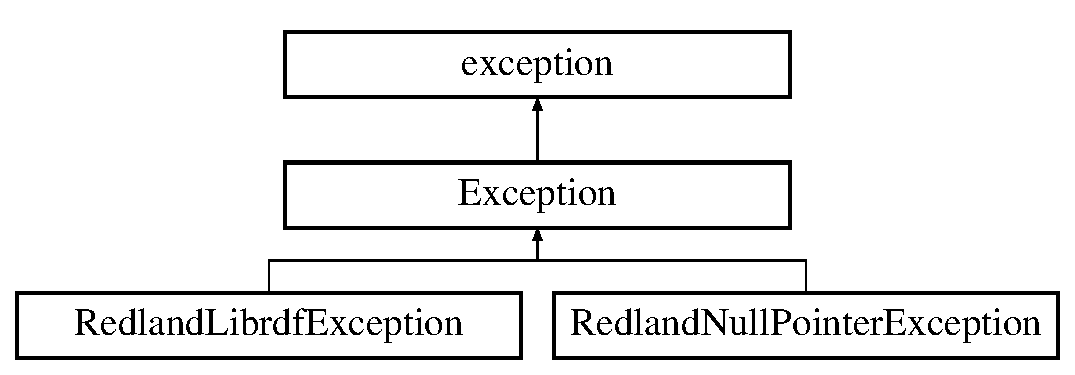
\includegraphics[height=3.000000cm]{classException}
\end{center}
\end{figure}
\subsection*{Public Member Functions}
\begin{DoxyCompactItemize}
\item 
\hyperlink{classException_ac541ead5c20548813d7dea73c28c7fab}{Exception} (const char $\ast$message)
\item 
\hyperlink{classException_a0b1693d4d5007815322070c907ee5cc2}{Exception} (std\+::string message)
\item 
\hyperlink{classException_ab834fdbc275748cf287b994503521ada}{$\sim$\+Exception} () noexcept override=default
\item 
const char $\ast$ \hyperlink{classException_ae7ba8334eb35e001b4b0c6df9339c0dc}{what} () const noexcept override
\end{DoxyCompactItemize}
\subsection*{Protected Attributes}
\begin{DoxyCompactItemize}
\item 
std\+::string \hyperlink{classException_a5d59cc46086c61391ed26773ce861780}{msg\+\_\+}
\end{DoxyCompactItemize}


\subsection{Constructor \& Destructor Documentation}
\mbox{\Hypertarget{classException_ac541ead5c20548813d7dea73c28c7fab}\label{classException_ac541ead5c20548813d7dea73c28c7fab}} 
\index{Exception@{Exception}!Exception@{Exception}}
\index{Exception@{Exception}!Exception@{Exception}}
\subsubsection{\texorpdfstring{Exception()}{Exception()}\hspace{0.1cm}{\footnotesize\ttfamily [1/2]}}
{\footnotesize\ttfamily Exception\+::\+Exception (\begin{DoxyParamCaption}\item[{const char $\ast$}]{message }\end{DoxyParamCaption})\hspace{0.3cm}{\ttfamily [inline]}, {\ttfamily [explicit]}}

Constructor (C strings). 
\begin{DoxyParams}{Parameters}
{\em message} & C-\/style string error message. The string contents are copied upon construction. Hence, responsibility for deleting the char$\ast$ lies with the caller. \\
\hline
\end{DoxyParams}
\mbox{\Hypertarget{classException_a0b1693d4d5007815322070c907ee5cc2}\label{classException_a0b1693d4d5007815322070c907ee5cc2}} 
\index{Exception@{Exception}!Exception@{Exception}}
\index{Exception@{Exception}!Exception@{Exception}}
\subsubsection{\texorpdfstring{Exception()}{Exception()}\hspace{0.1cm}{\footnotesize\ttfamily [2/2]}}
{\footnotesize\ttfamily Exception\+::\+Exception (\begin{DoxyParamCaption}\item[{std\+::string}]{message }\end{DoxyParamCaption})\hspace{0.3cm}{\ttfamily [inline]}, {\ttfamily [explicit]}}

Constructor (C++ S\+TL strings). 
\begin{DoxyParams}{Parameters}
{\em message} & The error message. \\
\hline
\end{DoxyParams}
\mbox{\Hypertarget{classException_ab834fdbc275748cf287b994503521ada}\label{classException_ab834fdbc275748cf287b994503521ada}} 
\index{Exception@{Exception}!````~Exception@{$\sim$\+Exception}}
\index{````~Exception@{$\sim$\+Exception}!Exception@{Exception}}
\subsubsection{\texorpdfstring{$\sim$\+Exception()}{~Exception()}}
{\footnotesize\ttfamily Exception\+::$\sim$\+Exception (\begin{DoxyParamCaption}{ }\end{DoxyParamCaption})\hspace{0.3cm}{\ttfamily [override]}, {\ttfamily [default]}, {\ttfamily [noexcept]}}

Destructor. Virtual to allow for subclassing. 

\subsection{Member Function Documentation}
\mbox{\Hypertarget{classException_ae7ba8334eb35e001b4b0c6df9339c0dc}\label{classException_ae7ba8334eb35e001b4b0c6df9339c0dc}} 
\index{Exception@{Exception}!what@{what}}
\index{what@{what}!Exception@{Exception}}
\subsubsection{\texorpdfstring{what()}{what()}}
{\footnotesize\ttfamily const char$\ast$ Exception\+::what (\begin{DoxyParamCaption}{ }\end{DoxyParamCaption}) const\hspace{0.3cm}{\ttfamily [inline]}, {\ttfamily [override]}, {\ttfamily [noexcept]}}

Returns a pointer to the (constant) error description. \begin{DoxyReturn}{Returns}
A pointer to a const char$\ast$. The underlying memory is in posession of the \hyperlink{classException}{Exception} object. Callers must not attempt to free the memory. 
\end{DoxyReturn}


\subsection{Member Data Documentation}
\mbox{\Hypertarget{classException_a5d59cc46086c61391ed26773ce861780}\label{classException_a5d59cc46086c61391ed26773ce861780}} 
\index{Exception@{Exception}!msg\+\_\+@{msg\+\_\+}}
\index{msg\+\_\+@{msg\+\_\+}!Exception@{Exception}}
\subsubsection{\texorpdfstring{msg\+\_\+}{msg\_}}
{\footnotesize\ttfamily std\+::string Exception\+::msg\+\_\+\hspace{0.3cm}{\ttfamily [protected]}}

Error message. 

The documentation for this class was generated from the following file\+:\begin{DoxyCompactItemize}
\item 
src/redland/\+Redland\+Wrapper/src/Librdf\+Exception.\+h\end{DoxyCompactItemize}

\hypertarget{classomexmeta_1_1Foaf}{}\section{omexmeta\+:\+:Foaf Class Reference}
\label{classomexmeta_1_1Foaf}\index{omexmeta\+::\+Foaf@{omexmeta\+::\+Foaf}}
Inheritance diagram for omexmeta\+:\+:Foaf\+:\begin{figure}[H]
\begin{center}
\leavevmode
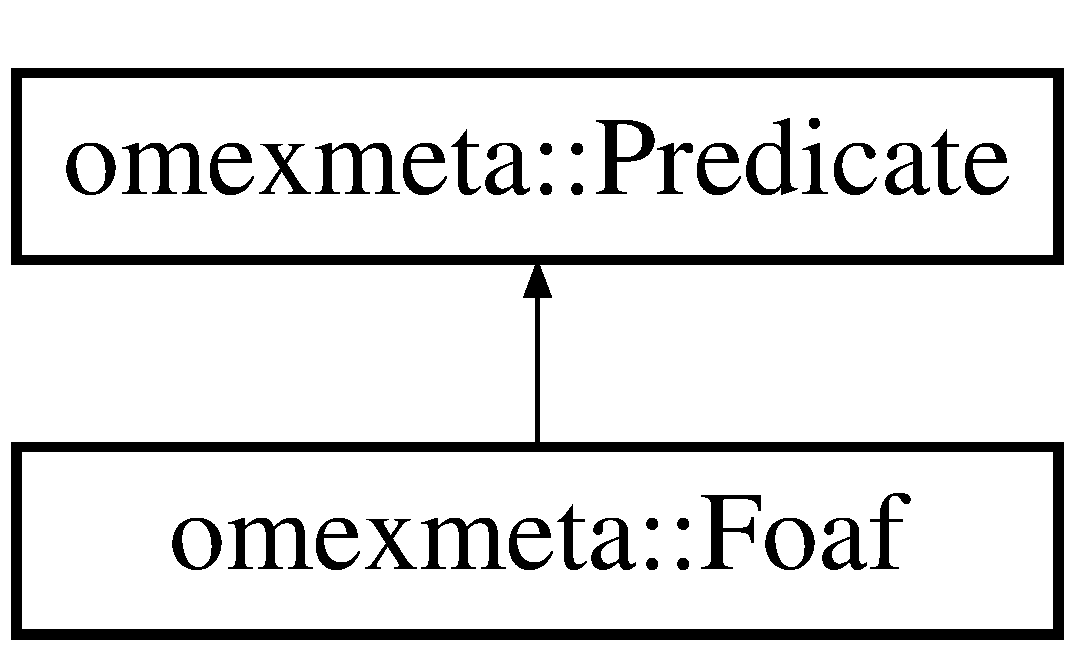
\includegraphics[height=2.000000cm]{classomexmeta_1_1Foaf}
\end{center}
\end{figure}
\subsection*{Public Member Functions}
\begin{DoxyCompactItemize}
\item 
\mbox{\Hypertarget{classomexmeta_1_1Foaf_af60965a79363573d9df78010936e1c81}\label{classomexmeta_1_1Foaf_af60965a79363573d9df78010936e1c81}} 
{\bfseries Foaf} (const std\+::string \&term)
\item 
\mbox{\Hypertarget{classomexmeta_1_1Foaf_a044d1eedbaf2be1ac6fcd160e3365a16}\label{classomexmeta_1_1Foaf_a044d1eedbaf2be1ac6fcd160e3365a16}} 
void {\bfseries verify} ()
\end{DoxyCompactItemize}
\subsection*{Public Attributes}
\begin{DoxyCompactItemize}
\item 
std\+::vector$<$ std\+::string $>$ {\bfseries valid\+\_\+terms\+\_\+}
\end{DoxyCompactItemize}
\subsection*{Additional Inherited Members}


\subsection{Member Data Documentation}
\mbox{\Hypertarget{classomexmeta_1_1Foaf_a5a91260f5319adc671c749a09ef0cf0a}\label{classomexmeta_1_1Foaf_a5a91260f5319adc671c749a09ef0cf0a}} 
\index{omexmeta\+::\+Foaf@{omexmeta\+::\+Foaf}!valid\+\_\+terms\+\_\+@{valid\+\_\+terms\+\_\+}}
\index{valid\+\_\+terms\+\_\+@{valid\+\_\+terms\+\_\+}!omexmeta\+::\+Foaf@{omexmeta\+::\+Foaf}}
\subsubsection{\texorpdfstring{valid\+\_\+terms\+\_\+}{valid\_terms\_}}
{\footnotesize\ttfamily std\+::vector$<$std\+::string$>$ omexmeta\+::\+Foaf\+::valid\+\_\+terms\+\_\+}

{\bfseries Initial value\+:}
\begin{DoxyCode}
\{
                \textcolor{stringliteral}{"Agent"}, \textcolor{stringliteral}{"Person"}, \textcolor{stringliteral}{"name"}, \textcolor{stringliteral}{"title"}, \textcolor{stringliteral}{"img"}, \textcolor{stringliteral}{"depiction"}, \textcolor{stringliteral}{"familyName"}, \textcolor{stringliteral}{"givenName"}, \textcolor{stringliteral}{"knows"},
                \textcolor{stringliteral}{"based\_near"}, \textcolor{stringliteral}{"age"}, \textcolor{stringliteral}{"made"}, \textcolor{stringliteral}{"primaryTopic"}, \textcolor{stringliteral}{"Project"}, \textcolor{stringliteral}{"Organization"}, \textcolor{stringliteral}{"Group"}, \textcolor{stringliteral}{"member"},
                \textcolor{stringliteral}{"Document"}, \textcolor{stringliteral}{"Image"}, \textcolor{stringliteral}{"nick"}, \textcolor{stringliteral}{"mbox"}, \textcolor{stringliteral}{"homepage"}, \textcolor{stringliteral}{"weblog"}, \textcolor{stringliteral}{"openid"}, \textcolor{stringliteral}{"jabberID"}, \textcolor{stringliteral}{"
      mbox\_sha1sum"},
                \textcolor{stringliteral}{"interest"}, \textcolor{stringliteral}{"topic\_interest"}, \textcolor{stringliteral}{"topic"}, \textcolor{stringliteral}{"workplaceHomepage"}, \textcolor{stringliteral}{"workInfoHomepage"}, \textcolor{stringliteral}{"
      schoolHomepage"},
                \textcolor{stringliteral}{"publications"}, \textcolor{stringliteral}{"currentProject"}, \textcolor{stringliteral}{"pastProject"}, \textcolor{stringliteral}{"account"}, \textcolor{stringliteral}{"OnlineAccount"}, \textcolor{stringliteral}{"accountName"},
                \textcolor{stringliteral}{"accountServiceHomepage"}, \textcolor{stringliteral}{"PersonalProfileDocument"}, \textcolor{stringliteral}{"tipjar"}, \textcolor{stringliteral}{"sha1"}, \textcolor{stringliteral}{"thumbnail"}, \textcolor{stringliteral}{"logo"},
      \}
\end{DoxyCode}


The documentation for this class was generated from the following files\+:\begin{DoxyCompactItemize}
\item 
src/omexmeta/Predicate.\+h\item 
src/omexmeta/Predicate.\+cpp\end{DoxyCompactItemize}

\hypertarget{structdbg_1_1detail_1_1has__ostream__operator}{}\section{dbg\+:\+:detail\+:\+:has\+\_\+ostream\+\_\+operator$<$ T $>$ Struct Template Reference}
\label{structdbg_1_1detail_1_1has__ostream__operator}\index{dbg\+::detail\+::has\+\_\+ostream\+\_\+operator$<$ T $>$@{dbg\+::detail\+::has\+\_\+ostream\+\_\+operator$<$ T $>$}}
Inheritance diagram for dbg\+:\+:detail\+:\+:has\+\_\+ostream\+\_\+operator$<$ T $>$\+:\begin{figure}[H]
\begin{center}
\leavevmode
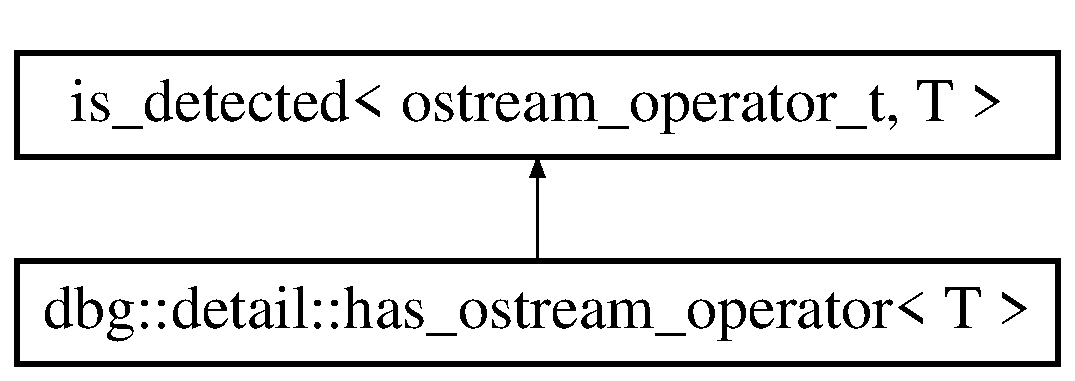
\includegraphics[height=2.000000cm]{structdbg_1_1detail_1_1has__ostream__operator}
\end{center}
\end{figure}


The documentation for this struct was generated from the following file\+:\begin{DoxyCompactItemize}
\item 
src/omexmeta/dbg.\+h\end{DoxyCompactItemize}

\hypertarget{classomexmeta_1_1InappropriateResourceException}{}\section{omexmeta\+:\+:Inappropriate\+Resource\+Exception Class Reference}
\label{classomexmeta_1_1InappropriateResourceException}\index{omexmeta\+::\+Inappropriate\+Resource\+Exception@{omexmeta\+::\+Inappropriate\+Resource\+Exception}}
Inheritance diagram for omexmeta\+:\+:Inappropriate\+Resource\+Exception\+:\begin{figure}[H]
\begin{center}
\leavevmode
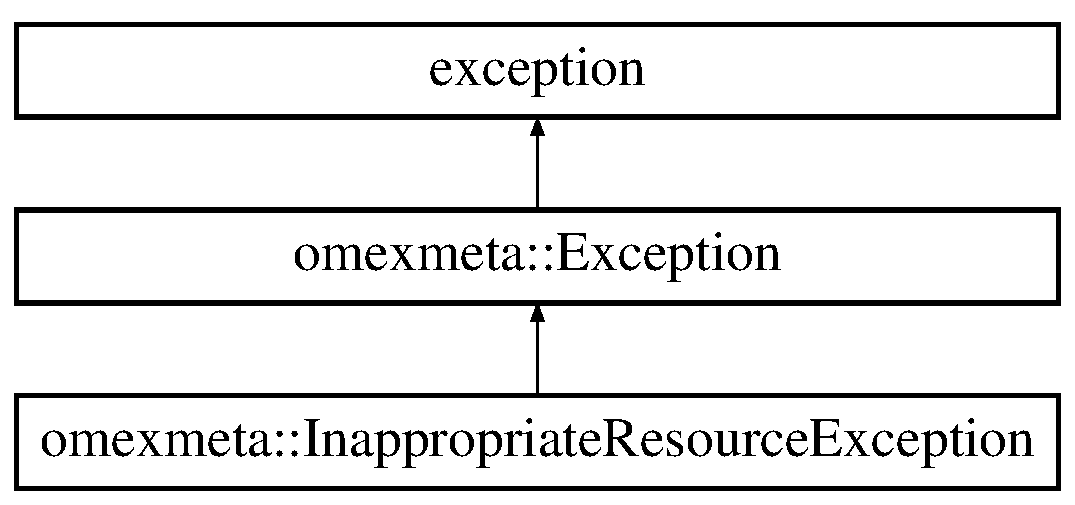
\includegraphics[height=3.000000cm]{classomexmeta_1_1InappropriateResourceException}
\end{center}
\end{figure}
\subsection*{Additional Inherited Members}


The documentation for this class was generated from the following file\+:\begin{DoxyCompactItemize}
\item 
src/omexmeta/Error.\+h\end{DoxyCompactItemize}

\hypertarget{structdbg_1_1detail_1_1is__container}{}\section{dbg\+:\+:detail\+:\+:is\+\_\+container$<$ T $>$ Struct Template Reference}
\label{structdbg_1_1detail_1_1is__container}\index{dbg\+::detail\+::is\+\_\+container$<$ T $>$@{dbg\+::detail\+::is\+\_\+container$<$ T $>$}}
\subsection*{Static Public Attributes}
\begin{DoxyCompactItemize}
\item 
static constexpr bool {\bfseries value}
\end{DoxyCompactItemize}


\subsection{Member Data Documentation}
\mbox{\Hypertarget{structdbg_1_1detail_1_1is__container_aa9a4594488352384b65b36198ac414f8}\label{structdbg_1_1detail_1_1is__container_aa9a4594488352384b65b36198ac414f8}} 
\index{dbg\+::detail\+::is\+\_\+container@{dbg\+::detail\+::is\+\_\+container}!value@{value}}
\index{value@{value}!dbg\+::detail\+::is\+\_\+container@{dbg\+::detail\+::is\+\_\+container}}
\subsubsection{\texorpdfstring{value}{value}}
{\footnotesize\ttfamily template$<$typename T $>$ \\
constexpr bool \hyperlink{structdbg_1_1detail_1_1is__container}{dbg\+::detail\+::is\+\_\+container}$<$ T $>$\+::value\hspace{0.3cm}{\ttfamily [static]}}

{\bfseries Initial value\+:}
\begin{DoxyCode}
=
      is\_detected<detect\_begin\_t, T>::value &&
      is\_detected<detect\_end\_t, T>::value &&
      is\_detected<detect\_size\_t, T>::value &&
      !std::is\_same<std::string,
                    \textcolor{keyword}{typename} std::remove\_cv<
                        \textcolor{keyword}{typename} std::remove\_reference<T>::type>::type>::value
\end{DoxyCode}


The documentation for this struct was generated from the following file\+:\begin{DoxyCompactItemize}
\item 
src/omexmeta/dbg.\+h\end{DoxyCompactItemize}

\hypertarget{structdbg_1_1last}{}\section{dbg\+:\+:last$<$ T, U $>$ Struct Template Reference}
\label{structdbg_1_1last}\index{dbg\+::last$<$ T, U $>$@{dbg\+::last$<$ T, U $>$}}
\subsection*{Public Types}
\begin{DoxyCompactItemize}
\item 
\mbox{\Hypertarget{structdbg_1_1last_aac2d6dd66fecfc0f3f37ecb4a02b0779}\label{structdbg_1_1last_aac2d6dd66fecfc0f3f37ecb4a02b0779}} 
using {\bfseries type} = typename \hyperlink{structdbg_1_1last}{last}$<$ U... $>$\+::type
\end{DoxyCompactItemize}


The documentation for this struct was generated from the following file\+:\begin{DoxyCompactItemize}
\item 
src/omexmeta/dbg.\+h\end{DoxyCompactItemize}

\hypertarget{structdbg_1_1last_3_01T_01_4}{}\section{dbg\+:\+:last$<$ T $>$ Struct Template Reference}
\label{structdbg_1_1last_3_01T_01_4}\index{dbg\+::last$<$ T $>$@{dbg\+::last$<$ T $>$}}
\subsection*{Public Types}
\begin{DoxyCompactItemize}
\item 
\mbox{\Hypertarget{structdbg_1_1last_3_01T_01_4_a6715c2f60dfaa8a096517ce45ff43999}\label{structdbg_1_1last_3_01T_01_4_a6715c2f60dfaa8a096517ce45ff43999}} 
using {\bfseries type} = T
\end{DoxyCompactItemize}


The documentation for this struct was generated from the following file\+:\begin{DoxyCompactItemize}
\item 
src/omexmeta/dbg.\+h\end{DoxyCompactItemize}

\hypertarget{classomexmeta_1_1LibRDFException}{}\section{omexmeta\+:\+:Lib\+R\+D\+F\+Exception Class Reference}
\label{classomexmeta_1_1LibRDFException}\index{omexmeta\+::\+Lib\+R\+D\+F\+Exception@{omexmeta\+::\+Lib\+R\+D\+F\+Exception}}
Inheritance diagram for omexmeta\+:\+:Lib\+R\+D\+F\+Exception\+:\begin{figure}[H]
\begin{center}
\leavevmode
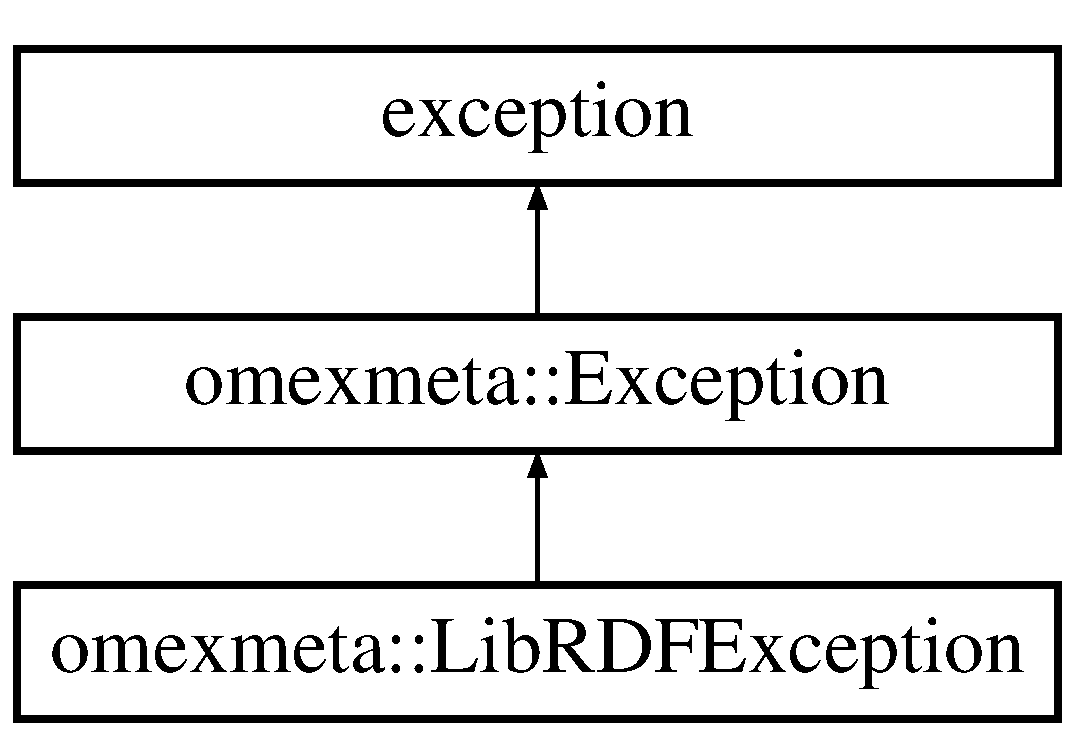
\includegraphics[height=3.000000cm]{classomexmeta_1_1LibRDFException}
\end{center}
\end{figure}
\subsection*{Additional Inherited Members}


The documentation for this class was generated from the following file\+:\begin{DoxyCompactItemize}
\item 
src/omexmeta/Error.\+h\end{DoxyCompactItemize}

\hypertarget{classredland_1_1LibrdfModel}{}\section{redland\+:\+:Librdf\+Model Class Reference}
\label{classredland_1_1LibrdfModel}\index{redland\+::\+Librdf\+Model@{redland\+::\+Librdf\+Model}}
\subsection*{Public Member Functions}
\begin{DoxyCompactItemize}
\item 
\mbox{\Hypertarget{classredland_1_1LibrdfModel_a1a8a3f9aad0520d6788aa2816ffb318e}\label{classredland_1_1LibrdfModel_a1a8a3f9aad0520d6788aa2816ffb318e}} 
bool {\bfseries operator==} (const \hyperlink{classredland_1_1LibrdfModel}{Librdf\+Model} \&rhs) const
\item 
\mbox{\Hypertarget{classredland_1_1LibrdfModel_a8cdaab0ea4c70808f015bfb6846b20bb}\label{classredland_1_1LibrdfModel_a8cdaab0ea4c70808f015bfb6846b20bb}} 
bool {\bfseries operator!=} (const \hyperlink{classredland_1_1LibrdfModel}{Librdf\+Model} \&rhs) const
\item 
\mbox{\Hypertarget{classredland_1_1LibrdfModel_a5a35c032585e38b1d41bc18f057128c1}\label{classredland_1_1LibrdfModel_a5a35c032585e38b1d41bc18f057128c1}} 
{\bfseries Librdf\+Model} (const \hyperlink{classredland_1_1LibrdfModel}{Librdf\+Model} \&model)=delete
\item 
\mbox{\Hypertarget{classredland_1_1LibrdfModel_a583e0eaecfe167ccbbeac5d768bcd644}\label{classredland_1_1LibrdfModel_a583e0eaecfe167ccbbeac5d768bcd644}} 
{\bfseries Librdf\+Model} (\hyperlink{classredland_1_1LibrdfModel}{Librdf\+Model} \&\&model) noexcept
\item 
\mbox{\Hypertarget{classredland_1_1LibrdfModel_a7bd07324b31fa8eb8f5f2e51b15044fc}\label{classredland_1_1LibrdfModel_a7bd07324b31fa8eb8f5f2e51b15044fc}} 
\hyperlink{classredland_1_1LibrdfModel}{Librdf\+Model} \& {\bfseries operator=} (const \hyperlink{classredland_1_1LibrdfModel}{Librdf\+Model} \&model)=delete
\item 
\mbox{\Hypertarget{classredland_1_1LibrdfModel_a9007acfb92943e018d20d6985c811033}\label{classredland_1_1LibrdfModel_a9007acfb92943e018d20d6985c811033}} 
\hyperlink{classredland_1_1LibrdfModel}{Librdf\+Model} \& {\bfseries operator=} (\hyperlink{classredland_1_1LibrdfModel}{Librdf\+Model} \&\&model) noexcept
\item 
\mbox{\Hypertarget{classredland_1_1LibrdfModel_a8b7d3063e030ce8613dcd6def7463a5a}\label{classredland_1_1LibrdfModel_a8b7d3063e030ce8613dcd6def7463a5a}} 
{\bfseries Librdf\+Model} (librdf\+\_\+model $\ast$model)
\item 
\mbox{\Hypertarget{classredland_1_1LibrdfModel_a355e16664fa50a8a3085f4070347106f}\label{classredland_1_1LibrdfModel_a355e16664fa50a8a3085f4070347106f}} 
{\bfseries Librdf\+Model} (librdf\+\_\+storage $\ast$storage, const char $\ast$options=nullptr)
\item 
\mbox{\Hypertarget{classredland_1_1LibrdfModel_ae1b996f1785adfe9b4a1824a73643248}\label{classredland_1_1LibrdfModel_ae1b996f1785adfe9b4a1824a73643248}} 
librdf\+\_\+model $\ast$ {\bfseries get} () const
\item 
\mbox{\Hypertarget{classredland_1_1LibrdfModel_a9bbced9329b4b9ef915789a37bf857b6}\label{classredland_1_1LibrdfModel_a9bbced9329b4b9ef915789a37bf857b6}} 
\hyperlink{classredland_1_1LibrdfQueryResults}{Librdf\+Query\+Results} {\bfseries query} (const \hyperlink{classredland_1_1LibrdfQuery}{Librdf\+Query} \&query) const
\item 
\mbox{\Hypertarget{classredland_1_1LibrdfModel_a646ed92896c4030de31c9e17b881bd2a}\label{classredland_1_1LibrdfModel_a646ed92896c4030de31c9e17b881bd2a}} 
\hyperlink{classredland_1_1LibrdfStream}{Librdf\+Stream} {\bfseries to\+Stream} ()
\item 
\mbox{\Hypertarget{classredland_1_1LibrdfModel_a3067eb5bae1353ab5c86f135c4b401ad}\label{classredland_1_1LibrdfModel_a3067eb5bae1353ab5c86f135c4b401ad}} 
int {\bfseries size} () const
\item 
\mbox{\Hypertarget{classredland_1_1LibrdfModel_a2b565a7d705e24d6163c068a40040087}\label{classredland_1_1LibrdfModel_a2b565a7d705e24d6163c068a40040087}} 
void {\bfseries add\+Statement} (const \hyperlink{classredland_1_1LibrdfStatement}{Librdf\+Statement} \&statement) const
\item 
\mbox{\Hypertarget{classredland_1_1LibrdfModel_a643c3e3d3363f4f06330ede73dc19514}\label{classredland_1_1LibrdfModel_a643c3e3d3363f4f06330ede73dc19514}} 
void {\bfseries add\+Statement} (librdf\+\_\+statement $\ast$statement) const
\item 
\mbox{\Hypertarget{classredland_1_1LibrdfModel_ad145b8f46be49434bb8bd0b90a904770}\label{classredland_1_1LibrdfModel_ad145b8f46be49434bb8bd0b90a904770}} 
void {\bfseries free\+Model} ()
\item 
\mbox{\Hypertarget{classredland_1_1LibrdfModel_a807784594a1515e5633ec7d08858dd57}\label{classredland_1_1LibrdfModel_a807784594a1515e5633ec7d08858dd57}} 
void {\bfseries remove\+Statement} (librdf\+\_\+statement $\ast$statement) const
\item 
\mbox{\Hypertarget{classredland_1_1LibrdfModel_a2cd4394b2c4fee69ce557eafd585c243}\label{classredland_1_1LibrdfModel_a2cd4394b2c4fee69ce557eafd585c243}} 
void {\bfseries remove\+Statement} (const \hyperlink{classredland_1_1LibrdfStatement}{Librdf\+Statement} \&statement) const
\item 
\mbox{\Hypertarget{classredland_1_1LibrdfModel_a6c40f1adbd292e5278ee6db5db356b34}\label{classredland_1_1LibrdfModel_a6c40f1adbd292e5278ee6db5db356b34}} 
librdf\+\_\+storage $\ast$ {\bfseries get\+Storage} () const
\item 
\mbox{\Hypertarget{classredland_1_1LibrdfModel_a21ddc6bf105a14ed3ad2a3bdfaf8c23d}\label{classredland_1_1LibrdfModel_a21ddc6bf105a14ed3ad2a3bdfaf8c23d}} 
int {\bfseries commit\+Transaction} () const
\item 
\mbox{\Hypertarget{classredland_1_1LibrdfModel_ac869cf4095da3cc748b52e30d6b5a95b}\label{classredland_1_1LibrdfModel_ac869cf4095da3cc748b52e30d6b5a95b}} 
int {\bfseries start\+Transaction} () const
\item 
\mbox{\Hypertarget{classredland_1_1LibrdfModel_ac6734571f6488dbabd4fdab2640f49b3}\label{classredland_1_1LibrdfModel_ac6734571f6488dbabd4fdab2640f49b3}} 
void $\ast$ {\bfseries get\+Transaction\+Handle} () const
\item 
\mbox{\Hypertarget{classredland_1_1LibrdfModel_a65b5be3bf67ef89173df06fc6190334e}\label{classredland_1_1LibrdfModel_a65b5be3bf67ef89173df06fc6190334e}} 
int {\bfseries start\+Transaction\+With\+Handle} (void $\ast$handle) const
\item 
\mbox{\Hypertarget{classredland_1_1LibrdfModel_abf9471d407147d24bbbda8c200d92791}\label{classredland_1_1LibrdfModel_abf9471d407147d24bbbda8c200d92791}} 
int {\bfseries get\+Transaction\+Rollback} () const
\item 
\mbox{\Hypertarget{classredland_1_1LibrdfModel_a3699be0e707d05cfabd88e31240707c4}\label{classredland_1_1LibrdfModel_a3699be0e707d05cfabd88e31240707c4}} 
void {\bfseries add\+Statement} (const librdf\+\_\+statement \&statement) const
\item 
\mbox{\Hypertarget{classredland_1_1LibrdfModel_a64915c9b196d061d1547f9a659177ea9}\label{classredland_1_1LibrdfModel_a64915c9b196d061d1547f9a659177ea9}} 
int {\bfseries supports\+Contexts} () const
\end{DoxyCompactItemize}


The documentation for this class was generated from the following files\+:\begin{DoxyCompactItemize}
\item 
src/redland/\+Redland\+Wrapper/src/Librdf\+Model.\+h\item 
src/redland/\+Redland\+Wrapper/src/Librdf\+Model.\+cpp\end{DoxyCompactItemize}

\hypertarget{classredland_1_1LibrdfNode}{}\section{redland\+:\+:Librdf\+Node Class Reference}
\label{classredland_1_1LibrdfNode}\index{redland\+::\+Librdf\+Node@{redland\+::\+Librdf\+Node}}
\subsection*{Public Member Functions}
\begin{DoxyCompactItemize}
\item 
\mbox{\Hypertarget{classredland_1_1LibrdfNode_afc1bdf57705253e8204a394541b96ca7}\label{classredland_1_1LibrdfNode_afc1bdf57705253e8204a394541b96ca7}} 
bool {\bfseries operator==} (const \hyperlink{classredland_1_1LibrdfNode}{Librdf\+Node} \&rhs) const
\item 
\mbox{\Hypertarget{classredland_1_1LibrdfNode_aefbf9e2bf34eb0171932e39323eadfd8}\label{classredland_1_1LibrdfNode_aefbf9e2bf34eb0171932e39323eadfd8}} 
bool {\bfseries operator!=} (const \hyperlink{classredland_1_1LibrdfNode}{Librdf\+Node} \&rhs) const
\item 
\mbox{\Hypertarget{classredland_1_1LibrdfNode_a28f6ce060bddf7e1cb88d17d4d4ea81a}\label{classredland_1_1LibrdfNode_a28f6ce060bddf7e1cb88d17d4d4ea81a}} 
void {\bfseries free\+Node} ()
\item 
\mbox{\Hypertarget{classredland_1_1LibrdfNode_a669557dc1240dc17c3a7a3a61d2400d9}\label{classredland_1_1LibrdfNode_a669557dc1240dc17c3a7a3a61d2400d9}} 
{\bfseries Librdf\+Node} (const \hyperlink{classredland_1_1LibrdfNode}{Librdf\+Node} \&node)=delete
\item 
\mbox{\Hypertarget{classredland_1_1LibrdfNode_a822ce6a4221315abe5768b278b83d0e5}\label{classredland_1_1LibrdfNode_a822ce6a4221315abe5768b278b83d0e5}} 
{\bfseries Librdf\+Node} (\hyperlink{classredland_1_1LibrdfNode}{Librdf\+Node} \&\&node) noexcept
\item 
\mbox{\Hypertarget{classredland_1_1LibrdfNode_abce52c34cc89e48886cde07aa5e113c9}\label{classredland_1_1LibrdfNode_abce52c34cc89e48886cde07aa5e113c9}} 
\hyperlink{classredland_1_1LibrdfNode}{Librdf\+Node} \& {\bfseries operator=} (const \hyperlink{classredland_1_1LibrdfNode}{Librdf\+Node} \&node)=delete
\item 
\mbox{\Hypertarget{classredland_1_1LibrdfNode_a9de3a69b00958b2bb50646dbf0aa8d7e}\label{classredland_1_1LibrdfNode_a9de3a69b00958b2bb50646dbf0aa8d7e}} 
\hyperlink{classredland_1_1LibrdfNode}{Librdf\+Node} \& {\bfseries operator=} (\hyperlink{classredland_1_1LibrdfNode}{Librdf\+Node} \&\&node) noexcept
\item 
\mbox{\Hypertarget{classredland_1_1LibrdfNode_a200c7a67088e66d6fc73f52bdb51d2e9}\label{classredland_1_1LibrdfNode_a200c7a67088e66d6fc73f52bdb51d2e9}} 
{\bfseries Librdf\+Node} (librdf\+\_\+node $\ast$node)
\item 
\mbox{\Hypertarget{classredland_1_1LibrdfNode_a33162ea36efe451c100325816cf8613f}\label{classredland_1_1LibrdfNode_a33162ea36efe451c100325816cf8613f}} 
librdf\+\_\+node $\ast$ {\bfseries get} () const
\item 
\mbox{\Hypertarget{classredland_1_1LibrdfNode_a83ec604f27e71cea80ac49569a06ddfe}\label{classredland_1_1LibrdfNode_a83ec604f27e71cea80ac49569a06ddfe}} 
raptor\+\_\+term\+\_\+type {\bfseries get\+Raptor\+Term\+Type} ()
\item 
\mbox{\Hypertarget{classredland_1_1LibrdfNode_a535fbe1bc21ca9cd9b39b969bfd2e500}\label{classredland_1_1LibrdfNode_a535fbe1bc21ca9cd9b39b969bfd2e500}} 
std\+::string {\bfseries str} () const
\item 
\mbox{\Hypertarget{classredland_1_1LibrdfNode_a98487d5af58971d820fcb99c88d8712d}\label{classredland_1_1LibrdfNode_a98487d5af58971d820fcb99c88d8712d}} 
\hyperlink{classredland_1_1LibrdfUri}{Librdf\+Uri} {\bfseries get\+Literal\+Datatype} ()
\item 
\mbox{\Hypertarget{classredland_1_1LibrdfNode_a58b9962c783be77fd0d2cb7036bfdc6a}\label{classredland_1_1LibrdfNode_a58b9962c783be77fd0d2cb7036bfdc6a}} 
std\+::string {\bfseries get\+Literal\+Language} ()
\item 
\mbox{\Hypertarget{classredland_1_1LibrdfNode_a49431de8c3262ee56d533a5fe047ee00}\label{classredland_1_1LibrdfNode_a49431de8c3262ee56d533a5fe047ee00}} 
std\+::string {\bfseries get\+Blank\+Identifier} ()
\item 
\mbox{\Hypertarget{classredland_1_1LibrdfNode_a0dd2ff697c0753eddf7327f64390ed77}\label{classredland_1_1LibrdfNode_a0dd2ff697c0753eddf7327f64390ed77}} 
\hyperlink{classredland_1_1LibrdfUri}{Librdf\+Uri} {\bfseries get\+Uri} ()
\item 
\mbox{\Hypertarget{classredland_1_1LibrdfNode_a01aeb7675187379674746f803a1fbdc9}\label{classredland_1_1LibrdfNode_a01aeb7675187379674746f803a1fbdc9}} 
void {\bfseries set\+Uri} (const std\+::string \&uri)
\item 
\mbox{\Hypertarget{classredland_1_1LibrdfNode_a160db9f7c7636c339e12c26f519b8fff}\label{classredland_1_1LibrdfNode_a160db9f7c7636c339e12c26f519b8fff}} 
void {\bfseries set\+Literal\+Datatype} (const std\+::string \&datatype)
\item 
\mbox{\Hypertarget{classredland_1_1LibrdfNode_afd81499fe4125cc2f4c472d33fb6c8c0}\label{classredland_1_1LibrdfNode_afd81499fe4125cc2f4c472d33fb6c8c0}} 
void {\bfseries set\+Blank\+Identifier} (const std\+::string \&identifier)
\item 
\mbox{\Hypertarget{classredland_1_1LibrdfNode_a8ac1d280707f4405dc8865465028ae33}\label{classredland_1_1LibrdfNode_a8ac1d280707f4405dc8865465028ae33}} 
\hyperlink{classredland_1_1LibrdfNode}{Librdf\+Node} {\bfseries from\+Uri\+String} (const std\+::string \&uri\+\_\+string, const std\+::string \&local\+\_\+prefix)
\end{DoxyCompactItemize}
\subsection*{Static Public Member Functions}
\begin{DoxyCompactItemize}
\item 
\mbox{\Hypertarget{classredland_1_1LibrdfNode_a5c971e6daeca94c4eabddfa5f6e4c456}\label{classredland_1_1LibrdfNode_a5c971e6daeca94c4eabddfa5f6e4c456}} 
static void {\bfseries free\+Node} (librdf\+\_\+node $\ast$node)
\item 
\mbox{\Hypertarget{classredland_1_1LibrdfNode_aacf853ee60f9d706bc7e95fb426166bd}\label{classredland_1_1LibrdfNode_aacf853ee60f9d706bc7e95fb426166bd}} 
static \hyperlink{classredland_1_1LibrdfNode}{Librdf\+Node} {\bfseries from\+Uri\+String} (const std\+::string \&uri\+\_\+string)
\item 
\mbox{\Hypertarget{classredland_1_1LibrdfNode_a22ea96262be432e6abb5c1e28ede3071}\label{classredland_1_1LibrdfNode_a22ea96262be432e6abb5c1e28ede3071}} 
static \hyperlink{classredland_1_1LibrdfNode}{Librdf\+Node} {\bfseries from\+Blank} (const std\+::string \&blank)
\item 
\mbox{\Hypertarget{classredland_1_1LibrdfNode_a346fad618a010ef983ce24d62891de0e}\label{classredland_1_1LibrdfNode_a346fad618a010ef983ce24d62891de0e}} 
static \hyperlink{classredland_1_1LibrdfNode}{Librdf\+Node} {\bfseries from\+Literal} (const std\+::string \&literal, const std\+::string \&literal\+\_\+datatype\+\_\+uri=\char`\"{}string\char`\"{}, const std\+::string \&xml\+\_\+language=std\+::string())
\item 
\mbox{\Hypertarget{classredland_1_1LibrdfNode_aaeeeca26bafdaf7f118af3307a4768be}\label{classredland_1_1LibrdfNode_aaeeeca26bafdaf7f118af3307a4768be}} 
static \hyperlink{classredland_1_1LibrdfNode}{Librdf\+Node} {\bfseries new\+Empty\+Node} ()
\item 
\mbox{\Hypertarget{classredland_1_1LibrdfNode_aa6bf7e25e68e473f2f39cb7b4cb5f39b}\label{classredland_1_1LibrdfNode_aa6bf7e25e68e473f2f39cb7b4cb5f39b}} 
static std\+::string {\bfseries str} (librdf\+\_\+node $\ast$node)
\item 
\mbox{\Hypertarget{classredland_1_1LibrdfNode_a3242e29edb736ba0aa8ac42fd6b3ae58}\label{classredland_1_1LibrdfNode_a3242e29edb736ba0aa8ac42fd6b3ae58}} 
static std\+::string {\bfseries validate\+Literal\+Datatype} (const std\+::string \&literal\+\_\+datatype\+\_\+uri)
\item 
\mbox{\Hypertarget{classredland_1_1LibrdfNode_a46208d163a49bc7640a8b4c847e2a28b}\label{classredland_1_1LibrdfNode_a46208d163a49bc7640a8b4c847e2a28b}} 
static \hyperlink{classredland_1_1LibrdfNode}{Librdf\+Node} {\bfseries copy\+Node} (const \hyperlink{classredland_1_1LibrdfNode}{Librdf\+Node} \&node)
\item 
\mbox{\Hypertarget{classredland_1_1LibrdfNode_a872032a7516dd140f93a9f4af3e0abd9}\label{classredland_1_1LibrdfNode_a872032a7516dd140f93a9f4af3e0abd9}} 
static \hyperlink{classredland_1_1LibrdfNode}{Librdf\+Node} {\bfseries from\+Relative\+Uri} (const std\+::string \&uri\+\_\+string, const std\+::string \&base\+\_\+uri)
\end{DoxyCompactItemize}


The documentation for this class was generated from the following files\+:\begin{DoxyCompactItemize}
\item 
src/redland/\+Redland\+Wrapper/src/Librdf\+Node.\+h\item 
src/redland/\+Redland\+Wrapper/src/Librdf\+Node.\+cpp\end{DoxyCompactItemize}

\hypertarget{classredland_1_1LibrdfParser}{}\section{redland\+:\+:Librdf\+Parser Class Reference}
\label{classredland_1_1LibrdfParser}\index{redland\+::\+Librdf\+Parser@{redland\+::\+Librdf\+Parser}}
\subsection*{Public Member Functions}
\begin{DoxyCompactItemize}
\item 
\mbox{\Hypertarget{classredland_1_1LibrdfParser_a884b4e7cb05942390fba7765cfb3aec8}\label{classredland_1_1LibrdfParser_a884b4e7cb05942390fba7765cfb3aec8}} 
{\bfseries Librdf\+Parser} (const \hyperlink{classredland_1_1LibrdfParser}{Librdf\+Parser} \&parser)=delete
\item 
\mbox{\Hypertarget{classredland_1_1LibrdfParser_a8c75ee321bd82076491aa0d63d0664c8}\label{classredland_1_1LibrdfParser_a8c75ee321bd82076491aa0d63d0664c8}} 
{\bfseries Librdf\+Parser} (\hyperlink{classredland_1_1LibrdfParser}{Librdf\+Parser} \&\&parser) noexcept
\item 
\mbox{\Hypertarget{classredland_1_1LibrdfParser_aeee1312383f2e3f72e49076390a2a27b}\label{classredland_1_1LibrdfParser_aeee1312383f2e3f72e49076390a2a27b}} 
\hyperlink{classredland_1_1LibrdfParser}{Librdf\+Parser} \& {\bfseries operator=} (const \hyperlink{classredland_1_1LibrdfParser}{Librdf\+Parser} \&parser)=delete
\item 
\mbox{\Hypertarget{classredland_1_1LibrdfParser_a5a5e09075b43906c9161d453ac63ab8a}\label{classredland_1_1LibrdfParser_a5a5e09075b43906c9161d453ac63ab8a}} 
\hyperlink{classredland_1_1LibrdfParser}{Librdf\+Parser} \& {\bfseries operator=} (\hyperlink{classredland_1_1LibrdfParser}{Librdf\+Parser} \&\&parser) noexcept
\item 
\mbox{\Hypertarget{classredland_1_1LibrdfParser_ac1373b22444c108a2a67dbf24fa4ca92}\label{classredland_1_1LibrdfParser_ac1373b22444c108a2a67dbf24fa4ca92}} 
{\bfseries Librdf\+Parser} (librdf\+\_\+parser $\ast$parser)
\item 
\mbox{\Hypertarget{classredland_1_1LibrdfParser_ac594c85ec97a39cad1aa557c98c39eb1}\label{classredland_1_1LibrdfParser_ac594c85ec97a39cad1aa557c98c39eb1}} 
{\bfseries Librdf\+Parser} (std\+::string format, std\+::string mime\+\_\+type=std\+::string(), const std\+::string \&type\+\_\+uri=std\+::string())
\item 
\mbox{\Hypertarget{classredland_1_1LibrdfParser_aadb297b986879ca618d3092fe737d41c}\label{classredland_1_1LibrdfParser_aadb297b986879ca618d3092fe737d41c}} 
librdf\+\_\+parser $\ast$ {\bfseries get} () const
\item 
\mbox{\Hypertarget{classredland_1_1LibrdfParser_a1e2098e2c99ba886ab1521048258600c}\label{classredland_1_1LibrdfParser_a1e2098e2c99ba886ab1521048258600c}} 
int {\bfseries num\+Namespaces\+Seen} () const
\item 
\mbox{\Hypertarget{classredland_1_1LibrdfParser_aed92021f88bccfa26bf78c29797b4208}\label{classredland_1_1LibrdfParser_aed92021f88bccfa26bf78c29797b4208}} 
std\+::string {\bfseries get\+Namespaces\+Seen\+Uri} (int index) const
\item 
\mbox{\Hypertarget{classredland_1_1LibrdfParser_a86739506ba32a9a6da8b69711f1026db}\label{classredland_1_1LibrdfParser_a86739506ba32a9a6da8b69711f1026db}} 
void {\bfseries parse\+String} (const std\+::string \&rdf\+\_\+string, const \hyperlink{classredland_1_1LibrdfModel}{Librdf\+Model} \&model, const \hyperlink{classredland_1_1LibrdfUri}{Librdf\+Uri} \&base\+\_\+uri) const
\item 
\mbox{\Hypertarget{classredland_1_1LibrdfParser_a2a7ac5ac97b4bc5876db02f0b9c7b987}\label{classredland_1_1LibrdfParser_a2a7ac5ac97b4bc5876db02f0b9c7b987}} 
void {\bfseries parse\+String} (const std\+::string \&rdf\+\_\+string, const \hyperlink{classredland_1_1LibrdfModel}{Librdf\+Model} \&model, const std\+::string \&base\+\_\+uri) const
\item 
\mbox{\Hypertarget{classredland_1_1LibrdfParser_a14c24e47699166e3b5bd4141ebd946ff}\label{classredland_1_1LibrdfParser_a14c24e47699166e3b5bd4141ebd946ff}} 
void {\bfseries parse\+File} (const std\+::string \&filename\+\_\+uri, const \hyperlink{classredland_1_1LibrdfModel}{Librdf\+Model} \&model, const std\+::string \&local\+\_\+uri) const
\item 
\mbox{\Hypertarget{classredland_1_1LibrdfParser_a15ffb21bf48e486708eab820719827a6}\label{classredland_1_1LibrdfParser_a15ffb21bf48e486708eab820719827a6}} 
void {\bfseries parse\+File} (const std\+::string \&filename\+\_\+uri, const \hyperlink{classredland_1_1LibrdfModel}{Librdf\+Model} \&model) const
\item 
\mbox{\Hypertarget{classredland_1_1LibrdfParser_a733bf5d33a2d71bd6d7c201e1c952b04}\label{classredland_1_1LibrdfParser_a733bf5d33a2d71bd6d7c201e1c952b04}} 
void {\bfseries parse\+Uri} (const std\+::string \&uri\+\_\+string, const \hyperlink{classredland_1_1LibrdfModel}{Librdf\+Model} \&model) const
\item 
\mbox{\Hypertarget{classredland_1_1LibrdfParser_a89d1335343c9999db8207866de8202c1}\label{classredland_1_1LibrdfParser_a89d1335343c9999db8207866de8202c1}} 
std\+::string {\bfseries get\+Namespaces\+Seen\+Prefix} (int index) const
\item 
\mbox{\Hypertarget{classredland_1_1LibrdfParser_aaa813cd98f57703e2168e81cf1c8b356}\label{classredland_1_1LibrdfParser_aaa813cd98f57703e2168e81cf1c8b356}} 
std\+::string {\bfseries get\+Name} () const
\item 
\mbox{\Hypertarget{classredland_1_1LibrdfParser_a152feb7bf2aa291fc7ec48fe2769265a}\label{classredland_1_1LibrdfParser_a152feb7bf2aa291fc7ec48fe2769265a}} 
void {\bfseries set\+Name} (const char $\ast$name)
\item 
\mbox{\Hypertarget{classredland_1_1LibrdfParser_aacf1514391f15d3687a35352f1c0da3d}\label{classredland_1_1LibrdfParser_aacf1514391f15d3687a35352f1c0da3d}} 
std\+::string {\bfseries get\+Mime\+Type} () const
\item 
\mbox{\Hypertarget{classredland_1_1LibrdfParser_a8fe0e89950e9b71f86fa58e10eb475d8}\label{classredland_1_1LibrdfParser_a8fe0e89950e9b71f86fa58e10eb475d8}} 
void {\bfseries set\+Mime\+Type} (const char $\ast$mime\+Type)
\item 
\mbox{\Hypertarget{classredland_1_1LibrdfParser_ae6f233d632e3a515afe7afceabf4e5ef}\label{classredland_1_1LibrdfParser_ae6f233d632e3a515afe7afceabf4e5ef}} 
librdf\+\_\+uri $\ast$ {\bfseries get\+Type\+Uri} () const
\item 
\mbox{\Hypertarget{classredland_1_1LibrdfParser_a81d772e0be266b00bf840fd9dbeab8d1}\label{classredland_1_1LibrdfParser_a81d772e0be266b00bf840fd9dbeab8d1}} 
void {\bfseries set\+Type\+Uri} (librdf\+\_\+uri $\ast$type\+Uri)
\item 
\mbox{\Hypertarget{classredland_1_1LibrdfParser_a76ecf31cd9fb96ba4e10a35f383e47fc}\label{classredland_1_1LibrdfParser_a76ecf31cd9fb96ba4e10a35f383e47fc}} 
void {\bfseries set\+Type\+Uri} (const std\+::string \&type\+\_\+uri)
\item 
\mbox{\Hypertarget{classredland_1_1LibrdfParser_a8055c22ada8b852112f4f011d9fa5abe}\label{classredland_1_1LibrdfParser_a8055c22ada8b852112f4f011d9fa5abe}} 
librdf\+\_\+parser $\ast$ {\bfseries make\+Parser} ()
\item 
\mbox{\Hypertarget{classredland_1_1LibrdfParser_a2c600b9ae3b59e4ae7e48b20e3513cb4}\label{classredland_1_1LibrdfParser_a2c600b9ae3b59e4ae7e48b20e3513cb4}} 
std\+::vector$<$ std\+::string $>$ {\bfseries get\+Seen\+Namespaces} () const
\end{DoxyCompactItemize}
\subsection*{Static Public Member Functions}
\begin{DoxyCompactItemize}
\item 
\mbox{\Hypertarget{classredland_1_1LibrdfParser_a9fa0b6b0d21fbc8c6dd0027b66a26eb5}\label{classredland_1_1LibrdfParser_a9fa0b6b0d21fbc8c6dd0027b66a26eb5}} 
static void {\bfseries set\+Feature} (librdf\+\_\+parser $\ast$parser, const std\+::string \&feature\+\_\+uri, librdf\+\_\+node $\ast$node)
\item 
\mbox{\Hypertarget{classredland_1_1LibrdfParser_aafc4a6e2748ee1175471ed0815d77eff}\label{classredland_1_1LibrdfParser_aafc4a6e2748ee1175471ed0815d77eff}} 
static void {\bfseries set\+Option} (librdf\+\_\+parser $\ast$parser, const std\+::string \&option, const std\+::string \&value)
\item 
\mbox{\Hypertarget{classredland_1_1LibrdfParser_a79fcda1e0c2cccfa8a070a1aea196ebd}\label{classredland_1_1LibrdfParser_a79fcda1e0c2cccfa8a070a1aea196ebd}} 
static void {\bfseries set\+Options} (librdf\+\_\+parser $\ast$parser)
\end{DoxyCompactItemize}


The documentation for this class was generated from the following files\+:\begin{DoxyCompactItemize}
\item 
src/redland/\+Redland\+Wrapper/src/Librdf\+Parser.\+h\item 
src/redland/\+Redland\+Wrapper/src/Librdf\+Parser.\+cpp\end{DoxyCompactItemize}

\hypertarget{classredland_1_1LibrdfQuery}{}\section{redland\+:\+:Librdf\+Query Class Reference}
\label{classredland_1_1LibrdfQuery}\index{redland\+::\+Librdf\+Query@{redland\+::\+Librdf\+Query}}
\subsection*{Public Member Functions}
\begin{DoxyCompactItemize}
\item 
\mbox{\Hypertarget{classredland_1_1LibrdfQuery_aacca5302206092fbd8908934d2236021}\label{classredland_1_1LibrdfQuery_aacca5302206092fbd8908934d2236021}} 
{\bfseries Librdf\+Query} (librdf\+\_\+query $\ast$query)
\item 
\mbox{\Hypertarget{classredland_1_1LibrdfQuery_a63a49930cc3c54938203683eab2c96fb}\label{classredland_1_1LibrdfQuery_a63a49930cc3c54938203683eab2c96fb}} 
{\bfseries Librdf\+Query} (const std\+::string \&query, const std\+::string \&name=\char`\"{}sparql\char`\"{}, const unsigned char $\ast$uri=nullptr, const char $\ast$base\+\_\+uri=nullptr)
\item 
\mbox{\Hypertarget{classredland_1_1LibrdfQuery_a0302f24051ae2050bc2e802a59364554}\label{classredland_1_1LibrdfQuery_a0302f24051ae2050bc2e802a59364554}} 
librdf\+\_\+query $\ast$ {\bfseries get} () const
\end{DoxyCompactItemize}


The documentation for this class was generated from the following files\+:\begin{DoxyCompactItemize}
\item 
src/redland/\+Redland\+Wrapper/src/Librdf\+Query.\+h\item 
src/redland/\+Redland\+Wrapper/src/Librdf\+Query.\+cpp\end{DoxyCompactItemize}

\hypertarget{classredland_1_1LibrdfQueryResults}{}\section{redland\+:\+:Librdf\+Query\+Results Class Reference}
\label{classredland_1_1LibrdfQueryResults}\index{redland\+::\+Librdf\+Query\+Results@{redland\+::\+Librdf\+Query\+Results}}
\subsection*{Public Member Functions}
\begin{DoxyCompactItemize}
\item 
\mbox{\Hypertarget{classredland_1_1LibrdfQueryResults_a8c9e17542c836ff3dd09da68bfc334f1}\label{classredland_1_1LibrdfQueryResults_a8c9e17542c836ff3dd09da68bfc334f1}} 
{\bfseries Librdf\+Query\+Results} (librdf\+\_\+query\+\_\+results $\ast$query\+Results)
\item 
\mbox{\Hypertarget{classredland_1_1LibrdfQueryResults_aa40ed7731b543dfc971b5acbb016cfee}\label{classredland_1_1LibrdfQueryResults_aa40ed7731b543dfc971b5acbb016cfee}} 
librdf\+\_\+query\+\_\+results $\ast$ {\bfseries get} () const
\item 
\mbox{\Hypertarget{classredland_1_1LibrdfQueryResults_acb51d92dfce59fdc64bd475326b038bf}\label{classredland_1_1LibrdfQueryResults_acb51d92dfce59fdc64bd475326b038bf}} 
std\+::string {\bfseries str} (std\+::string format)
\end{DoxyCompactItemize}


The documentation for this class was generated from the following files\+:\begin{DoxyCompactItemize}
\item 
src/redland/\+Redland\+Wrapper/src/Librdf\+Query\+Results.\+h\item 
src/redland/\+Redland\+Wrapper/src/Librdf\+Query\+Results.\+cpp\end{DoxyCompactItemize}

\hypertarget{classredland_1_1LibrdfSerializer}{}\section{redland\+:\+:Librdf\+Serializer Class Reference}
\label{classredland_1_1LibrdfSerializer}\index{redland\+::\+Librdf\+Serializer@{redland\+::\+Librdf\+Serializer}}
\subsection*{Public Member Functions}
\begin{DoxyCompactItemize}
\item 
\mbox{\Hypertarget{classredland_1_1LibrdfSerializer_a084920f2dadf9aff9abff2fbe4e302e9}\label{classredland_1_1LibrdfSerializer_a084920f2dadf9aff9abff2fbe4e302e9}} 
{\bfseries Librdf\+Serializer} (const \hyperlink{classredland_1_1LibrdfSerializer}{Librdf\+Serializer} \&serializer)=delete
\item 
\mbox{\Hypertarget{classredland_1_1LibrdfSerializer_ac0df7aa8f6a63de75d63f33d9eb3b201}\label{classredland_1_1LibrdfSerializer_ac0df7aa8f6a63de75d63f33d9eb3b201}} 
{\bfseries Librdf\+Serializer} (\hyperlink{classredland_1_1LibrdfSerializer}{Librdf\+Serializer} \&\&serializer) noexcept
\item 
\mbox{\Hypertarget{classredland_1_1LibrdfSerializer_a07c9ec356305e42c4990357dffb6bfd1}\label{classredland_1_1LibrdfSerializer_a07c9ec356305e42c4990357dffb6bfd1}} 
\hyperlink{classredland_1_1LibrdfSerializer}{Librdf\+Serializer} \& {\bfseries operator=} (const \hyperlink{classredland_1_1LibrdfSerializer}{Librdf\+Serializer} \&serializer)=delete
\item 
\mbox{\Hypertarget{classredland_1_1LibrdfSerializer_a3f1049838f6c9b3baee42fd1ab99d9e3}\label{classredland_1_1LibrdfSerializer_a3f1049838f6c9b3baee42fd1ab99d9e3}} 
\hyperlink{classredland_1_1LibrdfSerializer}{Librdf\+Serializer} \& {\bfseries operator=} (\hyperlink{classredland_1_1LibrdfSerializer}{Librdf\+Serializer} \&\&serializer) noexcept
\item 
\mbox{\Hypertarget{classredland_1_1LibrdfSerializer_aadcc241a243f87fce5152dc6420d1625}\label{classredland_1_1LibrdfSerializer_aadcc241a243f87fce5152dc6420d1625}} 
{\bfseries Librdf\+Serializer} (const char $\ast$format, const char $\ast$mime\+\_\+type=nullptr, const char $\ast$type\+\_\+uri=nullptr)
\item 
\mbox{\Hypertarget{classredland_1_1LibrdfSerializer_ab5ef7eaa294357a931b826acc1ab932f}\label{classredland_1_1LibrdfSerializer_ab5ef7eaa294357a931b826acc1ab932f}} 
librdf\+\_\+serializer $\ast$ {\bfseries get} () const
\item 
\mbox{\Hypertarget{classredland_1_1LibrdfSerializer_ab621a575b7244c9d39e756b5e133766b}\label{classredland_1_1LibrdfSerializer_ab621a575b7244c9d39e756b5e133766b}} 
void {\bfseries set\+Namespace} (const std\+::string \&ns, const std\+::string \&prefix) const
\item 
\mbox{\Hypertarget{classredland_1_1LibrdfSerializer_abe500f5c5a1de1bdac86ab196a002b46}\label{classredland_1_1LibrdfSerializer_abe500f5c5a1de1bdac86ab196a002b46}} 
void {\bfseries set\+Feature} (const std\+::string \&ns, const std\+::string \&prefix) const
\item 
\mbox{\Hypertarget{classredland_1_1LibrdfSerializer_ac205990ca1dbf0ff1e56ea45e82ec8d2}\label{classredland_1_1LibrdfSerializer_ac205990ca1dbf0ff1e56ea45e82ec8d2}} 
std\+::string {\bfseries to\+String} (const std\+::string \&uri, const \hyperlink{classredland_1_1LibrdfModel}{Librdf\+Model} \&model)
\item 
\mbox{\Hypertarget{classredland_1_1LibrdfSerializer_aa185a5c5708bf4b08dfa5eb6a8b897b1}\label{classredland_1_1LibrdfSerializer_aa185a5c5708bf4b08dfa5eb6a8b897b1}} 
void {\bfseries free\+Serializer} ()
\item 
\mbox{\Hypertarget{classredland_1_1LibrdfSerializer_a4ea50f1f63c3cb7bb63da3fc55994fee}\label{classredland_1_1LibrdfSerializer_a4ea50f1f63c3cb7bb63da3fc55994fee}} 
void {\bfseries validate\+Serializer\+Name} (std\+::string name)
\item 
\mbox{\Hypertarget{classredland_1_1LibrdfSerializer_a970fa3d23ba08a63533c758417de1808}\label{classredland_1_1LibrdfSerializer_a970fa3d23ba08a63533c758417de1808}} 
void {\bfseries set\+Option} (const std\+::string \&option, const std\+::string \&value) const
\item 
\mbox{\Hypertarget{classredland_1_1LibrdfSerializer_ad2cb2ddcd225119a2a9a33001da22478}\label{classredland_1_1LibrdfSerializer_ad2cb2ddcd225119a2a9a33001da22478}} 
void {\bfseries set\+Options} () const
\end{DoxyCompactItemize}
\subsection*{Static Public Member Functions}
\begin{DoxyCompactItemize}
\item 
\mbox{\Hypertarget{classredland_1_1LibrdfSerializer_a58915bb2aa6b7c0eb438b5cc0148ef45}\label{classredland_1_1LibrdfSerializer_a58915bb2aa6b7c0eb438b5cc0148ef45}} 
static \hyperlink{classredland_1_1LibrdfSerializer}{Librdf\+Serializer} {\bfseries from\+Raw\+Ptr} (librdf\+\_\+serializer $\ast$serializer)
\end{DoxyCompactItemize}


The documentation for this class was generated from the following files\+:\begin{DoxyCompactItemize}
\item 
src/redland/\+Redland\+Wrapper/src/Librdf\+Serializer.\+h\item 
src/redland/\+Redland\+Wrapper/src/Librdf\+Serializer.\+cpp\end{DoxyCompactItemize}

\hypertarget{classredland_1_1LibrdfStatement}{}\section{redland\+:\+:Librdf\+Statement Class Reference}
\label{classredland_1_1LibrdfStatement}\index{redland\+::\+Librdf\+Statement@{redland\+::\+Librdf\+Statement}}
Inheritance diagram for redland\+:\+:Librdf\+Statement\+:\begin{figure}[H]
\begin{center}
\leavevmode
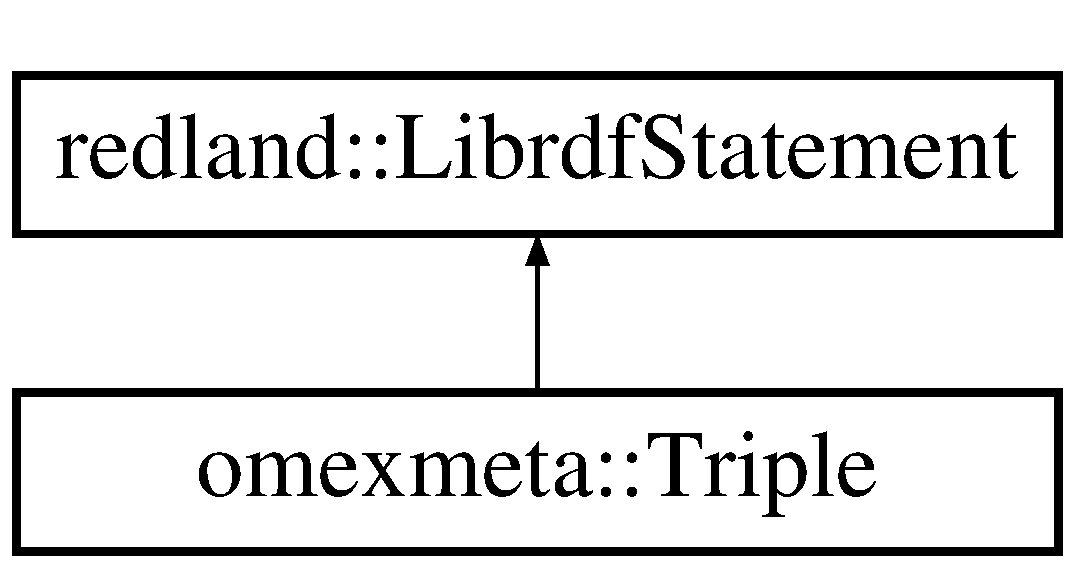
\includegraphics[height=2.000000cm]{classredland_1_1LibrdfStatement}
\end{center}
\end{figure}
\subsection*{Public Member Functions}
\begin{DoxyCompactItemize}
\item 
\mbox{\Hypertarget{classredland_1_1LibrdfStatement_ada81e9bfb312e25daf20d6dda10eeb2e}\label{classredland_1_1LibrdfStatement_ada81e9bfb312e25daf20d6dda10eeb2e}} 
bool {\bfseries operator==} (const \hyperlink{classredland_1_1LibrdfStatement}{Librdf\+Statement} \&rhs) const
\item 
\mbox{\Hypertarget{classredland_1_1LibrdfStatement_ad3d6c126b90c0d93413a08353c496f8f}\label{classredland_1_1LibrdfStatement_ad3d6c126b90c0d93413a08353c496f8f}} 
bool {\bfseries operator!=} (const \hyperlink{classredland_1_1LibrdfStatement}{Librdf\+Statement} \&rhs) const
\item 
\mbox{\Hypertarget{classredland_1_1LibrdfStatement_ae7f7e27b7a502070195103268407243a}\label{classredland_1_1LibrdfStatement_ae7f7e27b7a502070195103268407243a}} 
{\bfseries Librdf\+Statement} (const \hyperlink{classredland_1_1LibrdfNode}{Librdf\+Node} \&subject, const \hyperlink{classredland_1_1LibrdfNode}{Librdf\+Node} \&predicate, const \hyperlink{classredland_1_1LibrdfNode}{Librdf\+Node} \&resource)
\item 
\mbox{\Hypertarget{classredland_1_1LibrdfStatement_a344ec4a937a1d67589ebc7247b3f08c6}\label{classredland_1_1LibrdfStatement_a344ec4a937a1d67589ebc7247b3f08c6}} 
{\bfseries Librdf\+Statement} (const \hyperlink{classredland_1_1LibrdfStatement}{Librdf\+Statement} \&statement)=delete
\item 
\mbox{\Hypertarget{classredland_1_1LibrdfStatement_aea171565ffb3ecc8d9c1db5439314306}\label{classredland_1_1LibrdfStatement_aea171565ffb3ecc8d9c1db5439314306}} 
{\bfseries Librdf\+Statement} (\hyperlink{classredland_1_1LibrdfStatement}{Librdf\+Statement} \&\&statement) noexcept
\item 
\mbox{\Hypertarget{classredland_1_1LibrdfStatement_a7aeb5ac71f5583b5a56b4aad7d904381}\label{classredland_1_1LibrdfStatement_a7aeb5ac71f5583b5a56b4aad7d904381}} 
\hyperlink{classredland_1_1LibrdfStatement}{Librdf\+Statement} \& {\bfseries operator=} (const \hyperlink{classredland_1_1LibrdfStatement}{Librdf\+Statement} \&statement)=delete
\item 
\mbox{\Hypertarget{classredland_1_1LibrdfStatement_a6cebbcea1400ba2983b25096f3db3b3c}\label{classredland_1_1LibrdfStatement_a6cebbcea1400ba2983b25096f3db3b3c}} 
\hyperlink{classredland_1_1LibrdfStatement}{Librdf\+Statement} \& {\bfseries operator=} (\hyperlink{classredland_1_1LibrdfStatement}{Librdf\+Statement} \&\&statement) noexcept
\item 
\mbox{\Hypertarget{classredland_1_1LibrdfStatement_aa51bc647bc938a07bd6c16b4d6ce07b4}\label{classredland_1_1LibrdfStatement_aa51bc647bc938a07bd6c16b4d6ce07b4}} 
void {\bfseries free\+Statement} ()
\item 
\mbox{\Hypertarget{classredland_1_1LibrdfStatement_a6b655a56f37dbe95fec840a0a1f0ed53}\label{classredland_1_1LibrdfStatement_a6b655a56f37dbe95fec840a0a1f0ed53}} 
librdf\+\_\+statement $\ast$ {\bfseries get} () const
\item 
\mbox{\Hypertarget{classredland_1_1LibrdfStatement_abcf022b8e24a74282e1d059fdf54d3fe}\label{classredland_1_1LibrdfStatement_abcf022b8e24a74282e1d059fdf54d3fe}} 
librdf\+\_\+node $\ast$ {\bfseries get\+Subject} () const
\item 
\mbox{\Hypertarget{classredland_1_1LibrdfStatement_a5aae51ac0994552a13f2c9b90bec63d0}\label{classredland_1_1LibrdfStatement_a5aae51ac0994552a13f2c9b90bec63d0}} 
librdf\+\_\+node $\ast$ {\bfseries get\+Predicate} () const
\item 
\mbox{\Hypertarget{classredland_1_1LibrdfStatement_aa763688f20b712ddc655afe405d7691a}\label{classredland_1_1LibrdfStatement_aa763688f20b712ddc655afe405d7691a}} 
librdf\+\_\+node $\ast$ {\bfseries get\+Resource} () const
\item 
\mbox{\Hypertarget{classredland_1_1LibrdfStatement_a6feed51cdebe7c4f2430fcba0ae17f37}\label{classredland_1_1LibrdfStatement_a6feed51cdebe7c4f2430fcba0ae17f37}} 
std\+::string {\bfseries get\+Subject\+Str} () const
\item 
\mbox{\Hypertarget{classredland_1_1LibrdfStatement_a5dd0d6a2e9fe1bfcf5254aa7928cdfaf}\label{classredland_1_1LibrdfStatement_a5dd0d6a2e9fe1bfcf5254aa7928cdfaf}} 
std\+::string {\bfseries get\+Predicate\+Str} () const
\item 
\mbox{\Hypertarget{classredland_1_1LibrdfStatement_adc21321df7ccf186c262e83a4438e993}\label{classredland_1_1LibrdfStatement_adc21321df7ccf186c262e83a4438e993}} 
std\+::string {\bfseries get\+Resource\+Str} () const
\item 
\mbox{\Hypertarget{classredland_1_1LibrdfStatement_a700219b2fed175a96fecfbd905d20ab1}\label{classredland_1_1LibrdfStatement_a700219b2fed175a96fecfbd905d20ab1}} 
void {\bfseries check\+For\+Null} ()
\item 
\mbox{\Hypertarget{classredland_1_1LibrdfStatement_a5fa27f77859a4673e991b9e86f84d889}\label{classredland_1_1LibrdfStatement_a5fa27f77859a4673e991b9e86f84d889}} 
void {\bfseries set\+Subject} (librdf\+\_\+node $\ast$node)
\item 
\mbox{\Hypertarget{classredland_1_1LibrdfStatement_a8b8fd2999e80bd2912af2430503a557a}\label{classredland_1_1LibrdfStatement_a8b8fd2999e80bd2912af2430503a557a}} 
void {\bfseries set\+Resource} (librdf\+\_\+node $\ast$node)
\item 
\mbox{\Hypertarget{classredland_1_1LibrdfStatement_a3306876fb080f3d19fca806142f93f87}\label{classredland_1_1LibrdfStatement_a3306876fb080f3d19fca806142f93f87}} 
void {\bfseries set\+Predicate} (librdf\+\_\+node $\ast$node)
\item 
\mbox{\Hypertarget{classredland_1_1LibrdfStatement_a84a6fae7f1879c2f033001a9927627b0}\label{classredland_1_1LibrdfStatement_a84a6fae7f1879c2f033001a9927627b0}} 
bool {\bfseries is\+Complete} ()
\item 
\mbox{\Hypertarget{classredland_1_1LibrdfStatement_af8417e75a1ddb953c64c36b6028d3448}\label{classredland_1_1LibrdfStatement_af8417e75a1ddb953c64c36b6028d3448}} 
std\+::unordered\+\_\+map$<$ std\+::string, int $>$ {\bfseries get\+Usages} ()
\item 
\mbox{\Hypertarget{classredland_1_1LibrdfStatement_a1881b122993ff4a24f560b7b31ea3176}\label{classredland_1_1LibrdfStatement_a1881b122993ff4a24f560b7b31ea3176}} 
void {\bfseries print\+Usages} ()
\item 
\mbox{\Hypertarget{classredland_1_1LibrdfStatement_a104a61ca5a7568728273c071269e1882}\label{classredland_1_1LibrdfStatement_a104a61ca5a7568728273c071269e1882}} 
void {\bfseries free\+Statement\+And\+Uris} ()
\end{DoxyCompactItemize}
\subsection*{Static Public Member Functions}
\begin{DoxyCompactItemize}
\item 
\mbox{\Hypertarget{classredland_1_1LibrdfStatement_a9fb66c801d731ffce13e4d1381c49c29}\label{classredland_1_1LibrdfStatement_a9fb66c801d731ffce13e4d1381c49c29}} 
static \hyperlink{classredland_1_1LibrdfStatement}{Librdf\+Statement} {\bfseries from\+Raw\+Statement\+Ptr} (librdf\+\_\+statement $\ast$statement)
\item 
\mbox{\Hypertarget{classredland_1_1LibrdfStatement_a4eceaebc10deea27f4c75f7c8b4cccaf}\label{classredland_1_1LibrdfStatement_a4eceaebc10deea27f4c75f7c8b4cccaf}} 
static \hyperlink{classredland_1_1LibrdfStatement}{Librdf\+Statement} {\bfseries from\+Raw\+Node\+Ptrs} (librdf\+\_\+node $\ast$subject, librdf\+\_\+node $\ast$predicate, librdf\+\_\+node $\ast$resource)
\end{DoxyCompactItemize}
\subsection*{Protected Member Functions}
\begin{DoxyCompactItemize}
\item 
\mbox{\Hypertarget{classredland_1_1LibrdfStatement_afd63d6425b2130dbe4e76fdee4d7218b}\label{classredland_1_1LibrdfStatement_afd63d6425b2130dbe4e76fdee4d7218b}} 
void {\bfseries refresh\+Statement} ()
\item 
\mbox{\Hypertarget{classredland_1_1LibrdfStatement_a4cbbbf99d094cea4569324a8c67789fb}\label{classredland_1_1LibrdfStatement_a4cbbbf99d094cea4569324a8c67789fb}} 
{\bfseries Librdf\+Statement} (librdf\+\_\+statement $\ast$statement)
\item 
\mbox{\Hypertarget{classredland_1_1LibrdfStatement_ac1b38e67ff0b90ac54b27c4f5f5d9e12}\label{classredland_1_1LibrdfStatement_ac1b38e67ff0b90ac54b27c4f5f5d9e12}} 
{\bfseries Librdf\+Statement} (librdf\+\_\+node $\ast$subject, librdf\+\_\+node $\ast$predicate, librdf\+\_\+node $\ast$resource)
\end{DoxyCompactItemize}
\subsection*{Protected Attributes}
\begin{DoxyCompactItemize}
\item 
\mbox{\Hypertarget{classredland_1_1LibrdfStatement_acd1e53cd114c6744cf808174a9333ce5}\label{classredland_1_1LibrdfStatement_acd1e53cd114c6744cf808174a9333ce5}} 
librdf\+\_\+statement $\ast$ {\bfseries statement\+\_\+} = librdf\+\_\+new\+\_\+statement(World\+::get\+World())
\end{DoxyCompactItemize}


The documentation for this class was generated from the following files\+:\begin{DoxyCompactItemize}
\item 
src/redland/\+Redland\+Wrapper/src/Librdf\+Statement.\+h\item 
src/redland/\+Redland\+Wrapper/src/Librdf\+Statement.\+cpp\end{DoxyCompactItemize}

\hypertarget{classredland_1_1LibrdfStorage}{}\section{redland\+:\+:Librdf\+Storage Class Reference}
\label{classredland_1_1LibrdfStorage}\index{redland\+::\+Librdf\+Storage@{redland\+::\+Librdf\+Storage}}
\subsection*{Public Member Functions}
\begin{DoxyCompactItemize}
\item 
\mbox{\Hypertarget{classredland_1_1LibrdfStorage_a8e3250af4dea528dcf94865835cfb8ff}\label{classredland_1_1LibrdfStorage_a8e3250af4dea528dcf94865835cfb8ff}} 
{\bfseries Librdf\+Storage} (librdf\+\_\+storage $\ast$storage)
\item 
\mbox{\Hypertarget{classredland_1_1LibrdfStorage_a08c025b165113efe1163c7294b989755}\label{classredland_1_1LibrdfStorage_a08c025b165113efe1163c7294b989755}} 
{\bfseries Librdf\+Storage} (const std\+::string \&storage\+\_\+name=\char`\"{}memory\char`\"{}, const std\+::string \&name=\char`\"{}Semsim\+Store\char`\"{}, const char $\ast$options=nullptr)
\item 
\mbox{\Hypertarget{classredland_1_1LibrdfStorage_a182d617ba7ab1b5359ef2693a56b272e}\label{classredland_1_1LibrdfStorage_a182d617ba7ab1b5359ef2693a56b272e}} 
librdf\+\_\+storage $\ast$ {\bfseries get} () const
\item 
\mbox{\Hypertarget{classredland_1_1LibrdfStorage_a7b08e7afd5ac5f38a0ed4cfeb77a3b99}\label{classredland_1_1LibrdfStorage_a7b08e7afd5ac5f38a0ed4cfeb77a3b99}} 
void {\bfseries free\+Storage} ()
\item 
\mbox{\Hypertarget{classredland_1_1LibrdfStorage_a7cef1518384fd6592ee8521cb95eb25d}\label{classredland_1_1LibrdfStorage_a7cef1518384fd6592ee8521cb95eb25d}} 
{\bfseries Librdf\+Storage} (const \hyperlink{classredland_1_1LibrdfStorage}{Librdf\+Storage} \&storage)=delete
\item 
\mbox{\Hypertarget{classredland_1_1LibrdfStorage_a59184a87b901f1d3709d045d57311606}\label{classredland_1_1LibrdfStorage_a59184a87b901f1d3709d045d57311606}} 
{\bfseries Librdf\+Storage} (\hyperlink{classredland_1_1LibrdfStorage}{Librdf\+Storage} \&\&storage) noexcept
\item 
\mbox{\Hypertarget{classredland_1_1LibrdfStorage_a1366716bbd3a0e41979d632c532c71ec}\label{classredland_1_1LibrdfStorage_a1366716bbd3a0e41979d632c532c71ec}} 
\hyperlink{classredland_1_1LibrdfStorage}{Librdf\+Storage} \& {\bfseries operator=} (\hyperlink{classredland_1_1LibrdfStorage}{Librdf\+Storage} \&\&storage) noexcept
\item 
\mbox{\Hypertarget{classredland_1_1LibrdfStorage_a3782ab4a08a32bd23a38eaad9c980fe9}\label{classredland_1_1LibrdfStorage_a3782ab4a08a32bd23a38eaad9c980fe9}} 
int {\bfseries add\+Statement} (librdf\+\_\+statement $\ast$statement)
\item 
\mbox{\Hypertarget{classredland_1_1LibrdfStorage_ae5e7a3708936893c9e553cbdc23d643a}\label{classredland_1_1LibrdfStorage_ae5e7a3708936893c9e553cbdc23d643a}} 
int {\bfseries add\+Statement} (const \hyperlink{classredland_1_1LibrdfStatement}{Librdf\+Statement} \&statement)
\item 
\mbox{\Hypertarget{classredland_1_1LibrdfStorage_a31ecaace536dface7d4a667ccf8db06c}\label{classredland_1_1LibrdfStorage_a31ecaace536dface7d4a667ccf8db06c}} 
int {\bfseries size} ()
\item 
\mbox{\Hypertarget{classredland_1_1LibrdfStorage_afb361eb4addaf74b725d63fed2cb38e6}\label{classredland_1_1LibrdfStorage_afb361eb4addaf74b725d63fed2cb38e6}} 
int {\bfseries commit} ()
\item 
\mbox{\Hypertarget{classredland_1_1LibrdfStorage_a93cc1f3c7e7ff2a250c9b14f66f60e39}\label{classredland_1_1LibrdfStorage_a93cc1f3c7e7ff2a250c9b14f66f60e39}} 
void {\bfseries print\+Available\+Storages} ()
\end{DoxyCompactItemize}


The documentation for this class was generated from the following files\+:\begin{DoxyCompactItemize}
\item 
src/redland/\+Redland\+Wrapper/src/Librdf\+Storage.\+h\item 
src/redland/\+Redland\+Wrapper/src/Librdf\+Storage.\+cpp\end{DoxyCompactItemize}

\hypertarget{classredland_1_1LibrdfStream}{}\section{redland\+:\+:Librdf\+Stream Class Reference}
\label{classredland_1_1LibrdfStream}\index{redland\+::\+Librdf\+Stream@{redland\+::\+Librdf\+Stream}}
\subsection*{Public Member Functions}
\begin{DoxyCompactItemize}
\item 
\mbox{\Hypertarget{classredland_1_1LibrdfStream_aaa64a7ef8a26be8cf35f3b31d6e34a1b}\label{classredland_1_1LibrdfStream_aaa64a7ef8a26be8cf35f3b31d6e34a1b}} 
{\bfseries Librdf\+Stream} (librdf\+\_\+stream $\ast$stream)
\item 
\mbox{\Hypertarget{classredland_1_1LibrdfStream_a5b52659abdfc01e583e1b9941eec2c4b}\label{classredland_1_1LibrdfStream_a5b52659abdfc01e583e1b9941eec2c4b}} 
librdf\+\_\+stream $\ast$ {\bfseries get} () const
\end{DoxyCompactItemize}


The documentation for this class was generated from the following files\+:\begin{DoxyCompactItemize}
\item 
src/redland/\+Redland\+Wrapper/src/Librdf\+Stream.\+h\item 
src/redland/\+Redland\+Wrapper/src/Librdf\+Stream.\+cpp\end{DoxyCompactItemize}

\hypertarget{classredland_1_1LibrdfUri}{}\section{redland\+:\+:Librdf\+Uri Class Reference}
\label{classredland_1_1LibrdfUri}\index{redland\+::\+Librdf\+Uri@{redland\+::\+Librdf\+Uri}}
\subsection*{Public Member Functions}
\begin{DoxyCompactItemize}
\item 
\mbox{\Hypertarget{classredland_1_1LibrdfUri_a3630cf904c9e4546fb6d6c175ed6c66e}\label{classredland_1_1LibrdfUri_a3630cf904c9e4546fb6d6c175ed6c66e}} 
\hyperlink{classredland_1_1LibrdfUri}{Librdf\+Uri} {\bfseries concatonate} (const std\+::string \&local\+\_\+name) const
\item 
\mbox{\Hypertarget{classredland_1_1LibrdfUri_acaeb8a0d4b6f493805ecc1b198807e1c}\label{classredland_1_1LibrdfUri_acaeb8a0d4b6f493805ecc1b198807e1c}} 
std\+::string {\bfseries str} () const
\item 
\mbox{\Hypertarget{classredland_1_1LibrdfUri_a36c5c589ae207ad6294e10be2bb8df17}\label{classredland_1_1LibrdfUri_a36c5c589ae207ad6294e10be2bb8df17}} 
{\bfseries Librdf\+Uri} (const std\+::string \&uri)
\item 
\mbox{\Hypertarget{classredland_1_1LibrdfUri_a1858bf7c3afae7d6d8ed2dca47e9cf55}\label{classredland_1_1LibrdfUri_a1858bf7c3afae7d6d8ed2dca47e9cf55}} 
librdf\+\_\+uri $\ast$ {\bfseries get} () const
\item 
\mbox{\Hypertarget{classredland_1_1LibrdfUri_ae9a8237bcb9cba0f2d87f2d980f579f3}\label{classredland_1_1LibrdfUri_ae9a8237bcb9cba0f2d87f2d980f579f3}} 
bool {\bfseries is\+Null} () const
\item 
\mbox{\Hypertarget{classredland_1_1LibrdfUri_a13f1a7bc775cd79b6bb4dc6cd31b5d53}\label{classredland_1_1LibrdfUri_a13f1a7bc775cd79b6bb4dc6cd31b5d53}} 
bool {\bfseries is\+Empty} () const
\item 
\mbox{\Hypertarget{classredland_1_1LibrdfUri_aa07e6315dc3428b6d864deb00cda48e1}\label{classredland_1_1LibrdfUri_aa07e6315dc3428b6d864deb00cda48e1}} 
void {\bfseries free\+Uri} ()
\item 
\mbox{\Hypertarget{classredland_1_1LibrdfUri_a770d47b63c041e39761f8dd46b0bf8b5}\label{classredland_1_1LibrdfUri_a770d47b63c041e39761f8dd46b0bf8b5}} 
bool {\bfseries is\+File\+Uri} () const
\item 
\mbox{\Hypertarget{classredland_1_1LibrdfUri_a02d802c21de7c9dba4133779701e3a45}\label{classredland_1_1LibrdfUri_a02d802c21de7c9dba4133779701e3a45}} 
bool {\bfseries operator==} (const \hyperlink{classredland_1_1LibrdfUri}{Librdf\+Uri} \&rhs) const
\item 
\mbox{\Hypertarget{classredland_1_1LibrdfUri_a8ded118526be9cfdbe6dbc87d075fb06}\label{classredland_1_1LibrdfUri_a8ded118526be9cfdbe6dbc87d075fb06}} 
bool {\bfseries operator!=} (const \hyperlink{classredland_1_1LibrdfUri}{Librdf\+Uri} \&rhs) const
\item 
\mbox{\Hypertarget{classredland_1_1LibrdfUri_ad24448f9b22adce080a35decc4694479}\label{classredland_1_1LibrdfUri_ad24448f9b22adce080a35decc4694479}} 
std\+::string {\bfseries to\+Filename\+String} () const
\item 
\mbox{\Hypertarget{classredland_1_1LibrdfUri_a77105fe3bed8bced2001bfee738f7032}\label{classredland_1_1LibrdfUri_a77105fe3bed8bced2001bfee738f7032}} 
int {\bfseries get\+Usage} ()
\end{DoxyCompactItemize}
\subsection*{Static Public Member Functions}
\begin{DoxyCompactItemize}
\item 
\mbox{\Hypertarget{classredland_1_1LibrdfUri_a518761e1fbfd8c2f79dcac01b05c720b}\label{classredland_1_1LibrdfUri_a518761e1fbfd8c2f79dcac01b05c720b}} 
static \hyperlink{classredland_1_1LibrdfUri}{Librdf\+Uri} {\bfseries from\+Raw\+Ptr} (librdf\+\_\+uri $\ast$uri)
\item 
\mbox{\Hypertarget{classredland_1_1LibrdfUri_ad7245bf32a2538d220ec7d3a0afc0802}\label{classredland_1_1LibrdfUri_ad7245bf32a2538d220ec7d3a0afc0802}} 
static \hyperlink{classredland_1_1LibrdfUri}{Librdf\+Uri} {\bfseries from\+Filename} (const std\+::string \&filename)
\item 
\mbox{\Hypertarget{classredland_1_1LibrdfUri_a58ab2ce202cc9b563d1dc60a20a545b2}\label{classredland_1_1LibrdfUri_a58ab2ce202cc9b563d1dc60a20a545b2}} 
static \hyperlink{classredland_1_1LibrdfUri}{Librdf\+Uri} {\bfseries concatonate} (librdf\+\_\+uri $\ast$old\+\_\+name, const std\+::string \&local\+\_\+name)
\end{DoxyCompactItemize}


The documentation for this class was generated from the following files\+:\begin{DoxyCompactItemize}
\item 
src/redland/\+Redland\+Wrapper/src/Librdf\+Uri.\+h\item 
src/redland/\+Redland\+Wrapper/src/Librdf\+Uri.\+cpp\end{DoxyCompactItemize}

\hypertarget{classomexmeta_1_1MarkupIdentifier}{}\section{omexmeta\+:\+:Markup\+Identifier Class Reference}
\label{classomexmeta_1_1MarkupIdentifier}\index{omexmeta\+::\+Markup\+Identifier@{omexmeta\+::\+Markup\+Identifier}}
\subsection*{Public Member Functions}
\begin{DoxyCompactItemize}
\item 
\mbox{\Hypertarget{classomexmeta_1_1MarkupIdentifier_a0bb73ce6d5c94efcd97471059a378058}\label{classomexmeta_1_1MarkupIdentifier_a0bb73ce6d5c94efcd97471059a378058}} 
{\bfseries Markup\+Identifier} (std\+::string markup)
\item 
\mbox{\Hypertarget{classomexmeta_1_1MarkupIdentifier_a541ffd197ce109e20112923d7fc0641b}\label{classomexmeta_1_1MarkupIdentifier_a541ffd197ce109e20112923d7fc0641b}} 
bool {\bfseries is\+S\+B\+ML} ()
\item 
\mbox{\Hypertarget{classomexmeta_1_1MarkupIdentifier_a2fd631a49a8a3d06e668cdbf130d5cb3}\label{classomexmeta_1_1MarkupIdentifier_a2fd631a49a8a3d06e668cdbf130d5cb3}} 
bool {\bfseries is\+Cell\+ML} ()
\item 
\mbox{\Hypertarget{classomexmeta_1_1MarkupIdentifier_ab1736abf0d275bcb6eefcb7f08dcbd4f}\label{classomexmeta_1_1MarkupIdentifier_ab1736abf0d275bcb6eefcb7f08dcbd4f}} 
const std\+::vector$<$ std\+::string $>$ \& {\bfseries get\+Element\+Names} () const
\end{DoxyCompactItemize}


The documentation for this class was generated from the following files\+:\begin{DoxyCompactItemize}
\item 
src/omexmeta/Markup\+Identifier.\+h\item 
src/omexmeta/Markup\+Identifier.\+cpp\end{DoxyCompactItemize}

\hypertarget{classomexmeta_1_1MediatorParticipant}{}\section{omexmeta\+:\+:Mediator\+Participant Class Reference}
\label{classomexmeta_1_1MediatorParticipant}\index{omexmeta\+::\+Mediator\+Participant@{omexmeta\+::\+Mediator\+Participant}}
Inheritance diagram for omexmeta\+:\+:Mediator\+Participant\+:\begin{figure}[H]
\begin{center}
\leavevmode
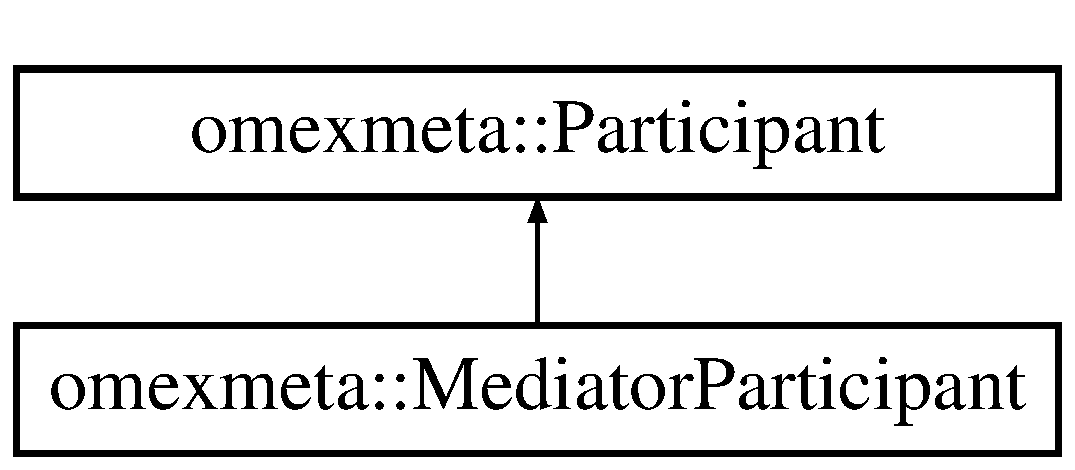
\includegraphics[height=2.000000cm]{classomexmeta_1_1MediatorParticipant}
\end{center}
\end{figure}
\subsection*{Public Member Functions}
\begin{DoxyCompactItemize}
\item 
\mbox{\Hypertarget{classomexmeta_1_1MediatorParticipant_a82d3e1fe6f987e1bf2ba838b75c9c3f0}\label{classomexmeta_1_1MediatorParticipant_a82d3e1fe6f987e1bf2ba838b75c9c3f0}} 
{\bfseries Mediator\+Participant} (librdf\+\_\+model $\ast$model, std\+::string physical\+Entity\+Reference, const std\+::string \&model\+\_\+uri, const std\+::string \&local\+\_\+uri)
\end{DoxyCompactItemize}


The documentation for this class was generated from the following files\+:\begin{DoxyCompactItemize}
\item 
src/omexmeta/Participant.\+h\item 
src/omexmeta/Participant.\+cpp\end{DoxyCompactItemize}

\hypertarget{classomexmeta_1_1MetaID}{}\section{omexmeta\+:\+:Meta\+ID Class Reference}
\label{classomexmeta_1_1MetaID}\index{omexmeta\+::\+Meta\+ID@{omexmeta\+::\+Meta\+ID}}
\subsection*{Public Member Functions}
\begin{DoxyCompactItemize}
\item 
\mbox{\Hypertarget{classomexmeta_1_1MetaID_af5cc076ccd6db8c411de98902d2a1218}\label{classomexmeta_1_1MetaID_af5cc076ccd6db8c411de98902d2a1218}} 
{\bfseries Meta\+ID} (std\+::string base, long start\+\_\+number, int num\+\_\+digits=4)
\item 
\mbox{\Hypertarget{classomexmeta_1_1MetaID_a3d6466efca8d9e931ca8c440c0809584}\label{classomexmeta_1_1MetaID_a3d6466efca8d9e931ca8c440c0809584}} 
bool {\bfseries operator==} (const \hyperlink{classomexmeta_1_1MetaID}{Meta\+ID} \&rhs) const
\item 
\mbox{\Hypertarget{classomexmeta_1_1MetaID_a25af693b284b0110914c537b48b20937}\label{classomexmeta_1_1MetaID_a25af693b284b0110914c537b48b20937}} 
bool {\bfseries operator!=} (const \hyperlink{classomexmeta_1_1MetaID}{Meta\+ID} \&rhs) const
\item 
\mbox{\Hypertarget{classomexmeta_1_1MetaID_a95e709df9b0ee47473bc40012738cdc8}\label{classomexmeta_1_1MetaID_a95e709df9b0ee47473bc40012738cdc8}} 
std\+::string {\bfseries generate} () const
\item 
\mbox{\Hypertarget{classomexmeta_1_1MetaID_a9a3c9b479d522e7630275d85582edd26}\label{classomexmeta_1_1MetaID_a9a3c9b479d522e7630275d85582edd26}} 
std\+::string {\bfseries generate} (long n) const
\item 
\mbox{\Hypertarget{classomexmeta_1_1MetaID_a343f4b48c9673f8943e03057370f01e4}\label{classomexmeta_1_1MetaID_a343f4b48c9673f8943e03057370f01e4}} 
int {\bfseries max\+Number} () const
\end{DoxyCompactItemize}
\subsection*{Static Public Member Functions}
\begin{DoxyCompactItemize}
\item 
\mbox{\Hypertarget{classomexmeta_1_1MetaID_ae4fe83a3512f64065e8e2997bc710be6}\label{classomexmeta_1_1MetaID_ae4fe83a3512f64065e8e2997bc710be6}} 
static int {\bfseries count\+Digits} (long long int n)
\end{DoxyCompactItemize}


The documentation for this class was generated from the following files\+:\begin{DoxyCompactItemize}
\item 
src/omexmeta/Meta\+I\+D.\+h\item 
src/omexmeta/Meta\+I\+D.\+cpp\end{DoxyCompactItemize}

\hypertarget{structdbg_1_1detail__detector_1_1nonesuch}{}\section{dbg\+:\+:detail\+\_\+detector\+:\+:nonesuch Struct Reference}
\label{structdbg_1_1detail__detector_1_1nonesuch}\index{dbg\+::detail\+\_\+detector\+::nonesuch@{dbg\+::detail\+\_\+detector\+::nonesuch}}
\subsection*{Public Member Functions}
\begin{DoxyCompactItemize}
\item 
\mbox{\Hypertarget{structdbg_1_1detail__detector_1_1nonesuch_a82c9bfc90b56b542819d8df5af7cebe6}\label{structdbg_1_1detail__detector_1_1nonesuch_a82c9bfc90b56b542819d8df5af7cebe6}} 
{\bfseries nonesuch} (\hyperlink{structdbg_1_1detail__detector_1_1nonesuch}{nonesuch} const \&)=delete
\item 
\mbox{\Hypertarget{structdbg_1_1detail__detector_1_1nonesuch_af0d1b2ab32ace678e2c9d95684d1917b}\label{structdbg_1_1detail__detector_1_1nonesuch_af0d1b2ab32ace678e2c9d95684d1917b}} 
void {\bfseries operator=} (\hyperlink{structdbg_1_1detail__detector_1_1nonesuch}{nonesuch} const \&)=delete
\end{DoxyCompactItemize}


The documentation for this struct was generated from the following file\+:\begin{DoxyCompactItemize}
\item 
src/omexmeta/dbg.\+h\end{DoxyCompactItemize}

\hypertarget{classomexmeta_1_1NotImplementedException}{}\section{omexmeta\+:\+:Not\+Implemented\+Exception Class Reference}
\label{classomexmeta_1_1NotImplementedException}\index{omexmeta\+::\+Not\+Implemented\+Exception@{omexmeta\+::\+Not\+Implemented\+Exception}}
Inheritance diagram for omexmeta\+:\+:Not\+Implemented\+Exception\+:\begin{figure}[H]
\begin{center}
\leavevmode
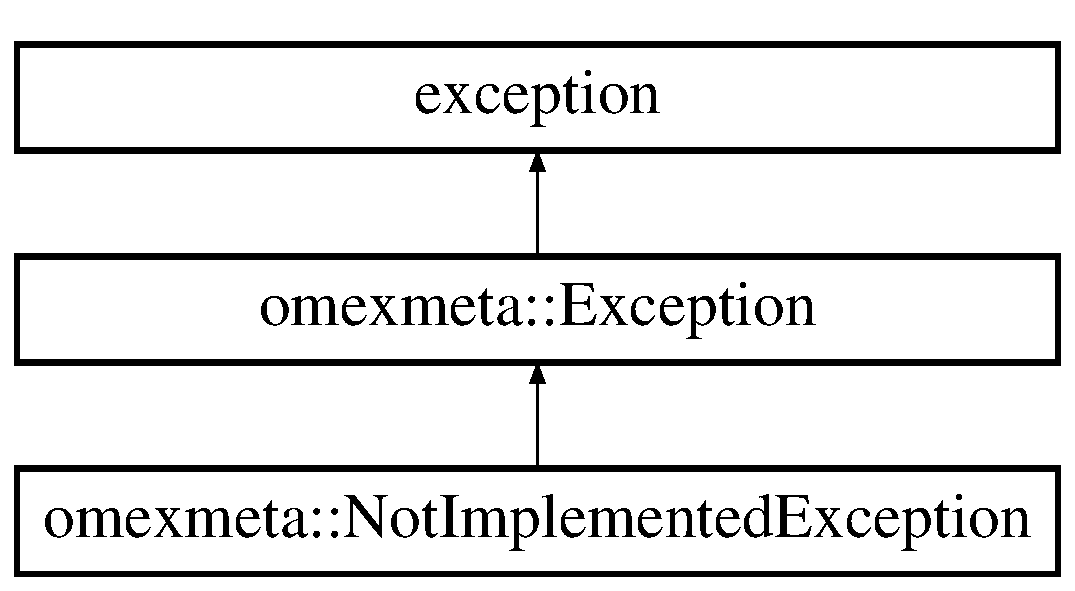
\includegraphics[height=3.000000cm]{classomexmeta_1_1NotImplementedException}
\end{center}
\end{figure}
\subsection*{Additional Inherited Members}


The documentation for this class was generated from the following file\+:\begin{DoxyCompactItemize}
\item 
src/omexmeta/Error.\+h\end{DoxyCompactItemize}

\hypertarget{classomexmeta_1_1NullPointerException}{}\section{omexmeta\+:\+:Null\+Pointer\+Exception Class Reference}
\label{classomexmeta_1_1NullPointerException}\index{omexmeta\+::\+Null\+Pointer\+Exception@{omexmeta\+::\+Null\+Pointer\+Exception}}
Inheritance diagram for omexmeta\+:\+:Null\+Pointer\+Exception\+:\begin{figure}[H]
\begin{center}
\leavevmode
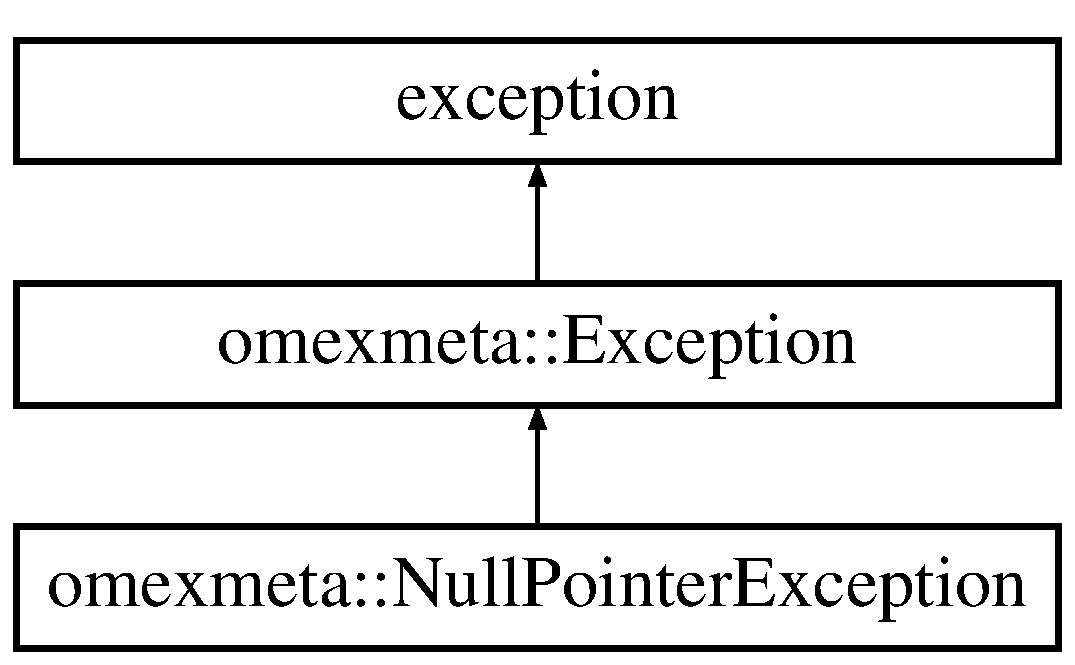
\includegraphics[height=3.000000cm]{classomexmeta_1_1NullPointerException}
\end{center}
\end{figure}
\subsection*{Additional Inherited Members}


The documentation for this class was generated from the following file\+:\begin{DoxyCompactItemize}
\item 
src/omexmeta/Error.\+h\end{DoxyCompactItemize}

\hypertarget{classomexmeta_1_1OmexMetaUtils}{}\section{omexmeta\+:\+:Omex\+Meta\+Utils Class Reference}
\label{classomexmeta_1_1OmexMetaUtils}\index{omexmeta\+::\+Omex\+Meta\+Utils@{omexmeta\+::\+Omex\+Meta\+Utils}}
\subsection*{Static Public Member Functions}
\begin{DoxyCompactItemize}
\item 
\mbox{\Hypertarget{classomexmeta_1_1OmexMetaUtils_ab72b362607e6bbdd0025eefa574cd073}\label{classomexmeta_1_1OmexMetaUtils_ab72b362607e6bbdd0025eefa574cd073}} 
static bool {\bfseries exists} (const std\+::string \&filename)
\item 
\mbox{\Hypertarget{classomexmeta_1_1OmexMetaUtils_a9c445a8e0cc6589b25d6fa630686c171}\label{classomexmeta_1_1OmexMetaUtils_a9c445a8e0cc6589b25d6fa630686c171}} 
static int {\bfseries remove\+File} (const std\+::string \&filename)
\item 
\mbox{\Hypertarget{classomexmeta_1_1OmexMetaUtils_a8e629136cb2685ed839ea3a0e88094e6}\label{classomexmeta_1_1OmexMetaUtils_a8e629136cb2685ed839ea3a0e88094e6}} 
static void {\bfseries remove\+If\+Exists} (const std\+::string \&filename)
\item 
\mbox{\Hypertarget{classomexmeta_1_1OmexMetaUtils_a046b603d6308242b70b55de6cb72325c}\label{classomexmeta_1_1OmexMetaUtils_a046b603d6308242b70b55de6cb72325c}} 
static void {\bfseries download} (const std\+::string \&url, std\+::string filename)
\item 
\mbox{\Hypertarget{classomexmeta_1_1OmexMetaUtils_aac769ce6e901f32820cd7dc3fef989fa}\label{classomexmeta_1_1OmexMetaUtils_aac769ce6e901f32820cd7dc3fef989fa}} 
static std\+::vector$<$ std\+::string $>$ {\bfseries split\+String\+By} (const std\+::string \&str, char delimiter)
\item 
\mbox{\Hypertarget{classomexmeta_1_1OmexMetaUtils_a4700231d455a5f65f7cc290d98d2b0ec}\label{classomexmeta_1_1OmexMetaUtils_a4700231d455a5f65f7cc290d98d2b0ec}} 
static std\+::string {\bfseries generate\+Unique\+Metaid} (librdf\+\_\+model $\ast$model, const std\+::string \&metaid\+\_\+base, std\+::vector$<$ std\+::string $>$ \&exclusions)
\item 
\mbox{\Hypertarget{classomexmeta_1_1OmexMetaUtils_a6694715cf3f5dccd33d416ecc84ff375}\label{classomexmeta_1_1OmexMetaUtils_a6694715cf3f5dccd33d416ecc84ff375}} 
static std\+::string {\bfseries prepare\+Base\+Uri} (std\+::string str, bool absolute\+\_\+path=false)
\item 
\mbox{\Hypertarget{classomexmeta_1_1OmexMetaUtils_a0956bde073b212596d8e4b2ffc983e47}\label{classomexmeta_1_1OmexMetaUtils_a0956bde073b212596d8e4b2ffc983e47}} 
static std\+::string {\bfseries get\+Namespace\+From\+Uri} (const std\+::string \&uri)
\item 
\mbox{\Hypertarget{classomexmeta_1_1OmexMetaUtils_af663724f2efb0324a64c6a57e8491c13}\label{classomexmeta_1_1OmexMetaUtils_af663724f2efb0324a64c6a57e8491c13}} 
static bool {\bfseries is\+Formatted\+Uri} (std\+::string uri)
\item 
\mbox{\Hypertarget{classomexmeta_1_1OmexMetaUtils_a9c2b712b85f74fff9740477660f7b371}\label{classomexmeta_1_1OmexMetaUtils_a9c2b712b85f74fff9740477660f7b371}} 
static bool {\bfseries ends\+With} (std\+::string const \&full\+\_\+string, std\+::string const \&ending)
\item 
\mbox{\Hypertarget{classomexmeta_1_1OmexMetaUtils_a4ec81c80bf33d232331ea9ef0b94da61}\label{classomexmeta_1_1OmexMetaUtils_a4ec81c80bf33d232331ea9ef0b94da61}} 
static bool {\bfseries assert\+Regex\+Match\+Split\+By\+New\+Line} (const std\+::string \&expected\+\_\+string, const std\+::string \&actual\+\_\+string)
\item 
\mbox{\Hypertarget{classomexmeta_1_1OmexMetaUtils_a6ddc16d56f238ef7ff3c8ab355163ef7}\label{classomexmeta_1_1OmexMetaUtils_a6ddc16d56f238ef7ff3c8ab355163ef7}} 
static bool {\bfseries assert\+Match\+By\+New\+Line} (const std\+::string \&expected\+\_\+string, const std\+::string \&actual\+\_\+string)
\item 
\mbox{\Hypertarget{classomexmeta_1_1OmexMetaUtils_a744a0575136f1cc60b76a6560a5595e9}\label{classomexmeta_1_1OmexMetaUtils_a744a0575136f1cc60b76a6560a5595e9}} 
static std\+::vector$<$ std\+::string $>$ {\bfseries configure\+Prefix\+Strings} (std\+::string repository\+\_\+name, std\+::string omex\+\_\+name, std\+::string model\+\_\+name)
\item 
\mbox{\Hypertarget{classomexmeta_1_1OmexMetaUtils_ae645af49ce57dac8bd0e0eba9e39a6c0}\label{classomexmeta_1_1OmexMetaUtils_ae645af49ce57dac8bd0e0eba9e39a6c0}} 
static std\+::string {\bfseries concat\+Meta\+Id\+And\+Uri} (std\+::string metaid, std\+::string uri)
\item 
\mbox{\Hypertarget{classomexmeta_1_1OmexMetaUtils_aca2230ca99338b9dc0fc7d296b0c553b}\label{classomexmeta_1_1OmexMetaUtils_aca2230ca99338b9dc0fc7d296b0c553b}} 
static std\+::string {\bfseries string\+Replace} (std\+::string str, const std\+::string \&string\+\_\+to\+\_\+replace, const std\+::string \&replacement)
\item 
\mbox{\Hypertarget{classomexmeta_1_1OmexMetaUtils_a66d58e0ebcbee1857b23ead70c87de7f}\label{classomexmeta_1_1OmexMetaUtils_a66d58e0ebcbee1857b23ead70c87de7f}} 
static bool {\bfseries starts\+With} (const std\+::string \&full\+\_\+string, const std\+::string \&start)
\item 
\mbox{\Hypertarget{classomexmeta_1_1OmexMetaUtils_a6f8e406b8798bd2f1f0ae0d1bd07ed2b}\label{classomexmeta_1_1OmexMetaUtils_a6f8e406b8798bd2f1f0ae0d1bd07ed2b}} 
static bool {\bfseries string\+In\+Vector} (std\+::vector$<$ std\+::string $>$ vec, const std\+::string \&string)
\item 
\mbox{\Hypertarget{classomexmeta_1_1OmexMetaUtils_a718710d8ba7fc7598bd73a5456b3d903}\label{classomexmeta_1_1OmexMetaUtils_a718710d8ba7fc7598bd73a5456b3d903}} 
static xml\+Doc $\ast$ {\bfseries parse\+Xml\+Document} (const std\+::string \&xml\+\_\+string)
\item 
\mbox{\Hypertarget{classomexmeta_1_1OmexMetaUtils_a29cc8222c809162eadbc424a0687cbf3}\label{classomexmeta_1_1OmexMetaUtils_a29cc8222c809162eadbc424a0687cbf3}} 
static std\+::string {\bfseries get\+Xml\+Node\+Property} (xml\+Node $\ast$node, const std\+::string \&property)
\item 
\mbox{\Hypertarget{classomexmeta_1_1OmexMetaUtils_a1dbcd874b2b72531e7f4f9e82524d8e8}\label{classomexmeta_1_1OmexMetaUtils_a1dbcd874b2b72531e7f4f9e82524d8e8}} 
static xml\+Node $\ast$ {\bfseries get\+Child\+Element\+Called} (xml\+Node $\ast$node, const std\+::string \&name)
\item 
\mbox{\Hypertarget{classomexmeta_1_1OmexMetaUtils_a4d6f7d2140c42435be9339edf975b949}\label{classomexmeta_1_1OmexMetaUtils_a4d6f7d2140c42435be9339edf975b949}} 
static std\+::vector$<$ xml\+Node $\ast$ $>$ {\bfseries get\+All\+Child\+Elements} (xml\+Node $\ast$node)
\item 
\mbox{\Hypertarget{classomexmeta_1_1OmexMetaUtils_a96e93667c8799b9569cb30fc102b129b}\label{classomexmeta_1_1OmexMetaUtils_a96e93667c8799b9569cb30fc102b129b}} 
static bool {\bfseries is\+Sub\+String} (const std\+::string \&full\+\_\+string, const std\+::string \&substring)
\end{DoxyCompactItemize}


The documentation for this class was generated from the following files\+:\begin{DoxyCompactItemize}
\item 
src/omexmeta/Omex\+Meta\+Utils.\+h\item 
src/omexmeta/Omex\+Meta\+Utils.\+cpp\end{DoxyCompactItemize}

\hypertarget{classomexmeta_1_1OmexMetaXmlAssistant}{}\section{omexmeta\+:\+:Omex\+Meta\+Xml\+Assistant Class Reference}
\label{classomexmeta_1_1OmexMetaXmlAssistant}\index{omexmeta\+::\+Omex\+Meta\+Xml\+Assistant@{omexmeta\+::\+Omex\+Meta\+Xml\+Assistant}}
Inheritance diagram for omexmeta\+:\+:Omex\+Meta\+Xml\+Assistant\+:\begin{figure}[H]
\begin{center}
\leavevmode
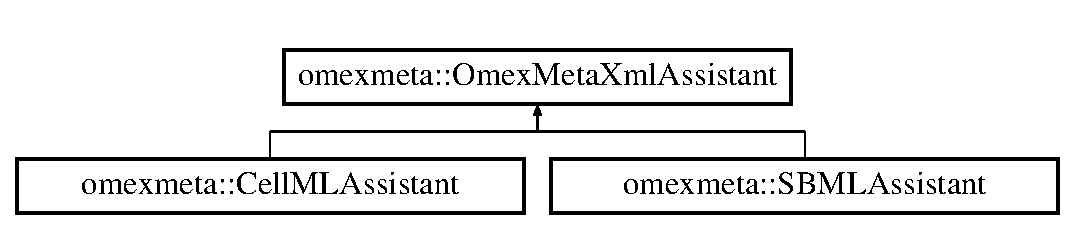
\includegraphics[height=2.000000cm]{classomexmeta_1_1OmexMetaXmlAssistant}
\end{center}
\end{figure}
\subsection*{Public Member Functions}
\begin{DoxyCompactItemize}
\item 
\mbox{\Hypertarget{classomexmeta_1_1OmexMetaXmlAssistant_a69bb3ac99f1585b6f567b80e88f52642}\label{classomexmeta_1_1OmexMetaXmlAssistant_a69bb3ac99f1585b6f567b80e88f52642}} 
const std\+::string \& {\bfseries get\+Metaid\+Base} () const
\item 
\mbox{\Hypertarget{classomexmeta_1_1OmexMetaXmlAssistant_a4c9759afd4af42595a4f0a4feb913524}\label{classomexmeta_1_1OmexMetaXmlAssistant_a4c9759afd4af42595a4f0a4feb913524}} 
int {\bfseries get\+Metaid\+Num\+Digits} () const
\item 
\mbox{\Hypertarget{classomexmeta_1_1OmexMetaXmlAssistant_a9ff89057f4fe7e8cb2e25f5431bf2bb5}\label{classomexmeta_1_1OmexMetaXmlAssistant_a9ff89057f4fe7e8cb2e25f5431bf2bb5}} 
bool {\bfseries generate\+New\+Metaids} () const
\item 
\mbox{\Hypertarget{classomexmeta_1_1OmexMetaXmlAssistant_af619a65dd28d04dfabd1930ff4110ce0}\label{classomexmeta_1_1OmexMetaXmlAssistant_af619a65dd28d04dfabd1930ff4110ce0}} 
{\bfseries Omex\+Meta\+Xml\+Assistant} (std\+::string xml, std\+::string metaid\+\_\+base=\char`\"{}Meta\+ID\char`\"{}, int metaid\+\_\+num\+\_\+digits=4, bool generate\+\_\+new\+\_\+metaids=false)
\item 
\mbox{\Hypertarget{classomexmeta_1_1OmexMetaXmlAssistant_aeef7e70a554aaf70fb694297e37e7cc8}\label{classomexmeta_1_1OmexMetaXmlAssistant_aeef7e70a554aaf70fb694297e37e7cc8}} 
std\+::pair$<$ std\+::string, std\+::vector$<$ std\+::string $>$ $>$ {\bfseries add\+Meta\+Ids} ()
\item 
\mbox{\Hypertarget{classomexmeta_1_1OmexMetaXmlAssistant_a3a6631e92df490f87f469abca81e1ba1}\label{classomexmeta_1_1OmexMetaXmlAssistant_a3a6631e92df490f87f469abca81e1ba1}} 
virtual std\+::vector$<$ std\+::string $>$ {\bfseries get\+Valid\+Elements} () const
\item 
\mbox{\Hypertarget{classomexmeta_1_1OmexMetaXmlAssistant_adbfc8d96f2adffa35ee01726a97dbcce}\label{classomexmeta_1_1OmexMetaXmlAssistant_adbfc8d96f2adffa35ee01726a97dbcce}} 
virtual std\+::string {\bfseries meta\+Id\+Tag\+Name} () const
\end{DoxyCompactItemize}


The documentation for this class was generated from the following files\+:\begin{DoxyCompactItemize}
\item 
src/omexmeta/Omex\+Meta\+Xml\+Assistant.\+h\item 
src/omexmeta/Omex\+Meta\+Xml\+Assistant.\+cpp\end{DoxyCompactItemize}

\hypertarget{classomexmeta_1_1Participant}{}\section{omexmeta\+:\+:Participant Class Reference}
\label{classomexmeta_1_1Participant}\index{omexmeta\+::\+Participant@{omexmeta\+::\+Participant}}
Inheritance diagram for omexmeta\+:\+:Participant\+:\begin{figure}[H]
\begin{center}
\leavevmode
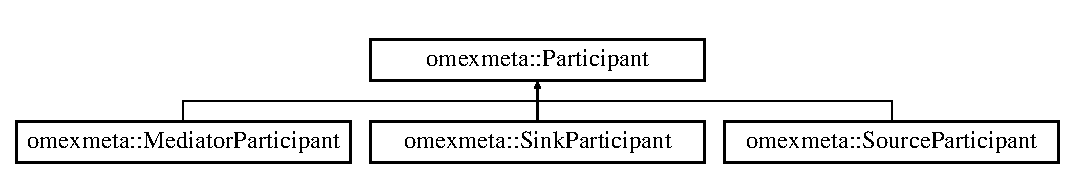
\includegraphics[height=1.954625cm]{classomexmeta_1_1Participant}
\end{center}
\end{figure}
\subsection*{Public Member Functions}
\begin{DoxyCompactItemize}
\item 
\mbox{\Hypertarget{classomexmeta_1_1Participant_a97c047d67dc86db1e617c3528bf8035e}\label{classomexmeta_1_1Participant_a97c047d67dc86db1e617c3528bf8035e}} 
void {\bfseries set\+Multiplier} (int multiplier)
\item 
\mbox{\Hypertarget{classomexmeta_1_1Participant_a415c1205762dff6943426d830d74edcd}\label{classomexmeta_1_1Participant_a415c1205762dff6943426d830d74edcd}} 
void {\bfseries set\+Physical\+Entity\+Reference} (const std\+::string \&physical\+Entity\+Reference)
\item 
\mbox{\Hypertarget{classomexmeta_1_1Participant_a8a6626e17aca48b76465d66928eee78f}\label{classomexmeta_1_1Participant_a8a6626e17aca48b76465d66928eee78f}} 
const std\+::string \& {\bfseries get\+Local\+Participant\+Metaid} () const
\item 
\mbox{\Hypertarget{classomexmeta_1_1Participant_a5e8f680950f55230587c0f85498c5047}\label{classomexmeta_1_1Participant_a5e8f680950f55230587c0f85498c5047}} 
void {\bfseries set\+Unique\+Participant\+Metaid} (const std\+::string \&unique\+Participant\+Metaid)
\item 
\mbox{\Hypertarget{classomexmeta_1_1Participant_a6bf4c724ab5212d10f2a89893f369cd1}\label{classomexmeta_1_1Participant_a6bf4c724ab5212d10f2a89893f369cd1}} 
const std\+::string \& {\bfseries get\+Local\+Uri} () const
\item 
\mbox{\Hypertarget{classomexmeta_1_1Participant_a595323ae0681f42a7ba5981e2ee840f1}\label{classomexmeta_1_1Participant_a595323ae0681f42a7ba5981e2ee840f1}} 
void {\bfseries set\+Local\+Uri} (const std\+::string \&local\+Uri)
\item 
\mbox{\Hypertarget{classomexmeta_1_1Participant_a395bc8d2561149a77371ed80e2ed1517}\label{classomexmeta_1_1Participant_a395bc8d2561149a77371ed80e2ed1517}} 
void {\bfseries free} ()
\item 
\mbox{\Hypertarget{classomexmeta_1_1Participant_a95c8c86650d1b0d31bb47eb618ff81b9}\label{classomexmeta_1_1Participant_a95c8c86650d1b0d31bb47eb618ff81b9}} 
{\bfseries Participant} (librdf\+\_\+model $\ast$model, std\+::string base\+\_\+metaid, const std\+::string \&model\+\_\+uri, const std\+::string \&local\+\_\+uri, std\+::string semsim\+\_\+predicate\+\_\+term, int multiplier, std\+::string physical\+Entity\+Reference)
\item 
\mbox{\Hypertarget{classomexmeta_1_1Participant_ad3db317039b403fdb7728885152cbeda}\label{classomexmeta_1_1Participant_ad3db317039b403fdb7728885152cbeda}} 
bool {\bfseries operator==} (const \hyperlink{classomexmeta_1_1Participant}{Participant} \&rhs) const
\item 
\mbox{\Hypertarget{classomexmeta_1_1Participant_aa4baa62cb4ccffe8443262382490328d}\label{classomexmeta_1_1Participant_aa4baa62cb4ccffe8443262382490328d}} 
bool {\bfseries operator!=} (const \hyperlink{classomexmeta_1_1Participant}{Participant} \&rhs) const
\item 
\mbox{\Hypertarget{classomexmeta_1_1Participant_a6757eea8a56972eb369e0e102ae5bfc8}\label{classomexmeta_1_1Participant_a6757eea8a56972eb369e0e102ae5bfc8}} 
\hyperlink{classomexmeta_1_1Triples}{Triples} {\bfseries to\+Triples} (const std\+::string \&subject\+\_\+metaid, std\+::vector$<$ std\+::string $>$ \&metaid\+\_\+exclusions)
\item 
\mbox{\Hypertarget{classomexmeta_1_1Participant_a03a1ffc7e9efaed5c0e94a62f7c72650}\label{classomexmeta_1_1Participant_a03a1ffc7e9efaed5c0e94a62f7c72650}} 
std\+::string {\bfseries create\+Metaid} (const std\+::string \&base, std\+::vector$<$ std\+::string $>$ \&metaid\+\_\+exclusions) const
\item 
\mbox{\Hypertarget{classomexmeta_1_1Participant_aa09f8c5736dd172b03d7898519d9478d}\label{classomexmeta_1_1Participant_aa09f8c5736dd172b03d7898519d9478d}} 
std\+::basic\+\_\+string$<$ char $>$ {\bfseries get\+Predicate} ()
\item 
\mbox{\Hypertarget{classomexmeta_1_1Participant_a1188d6a2036514eb6b649ce1e08eca4d}\label{classomexmeta_1_1Participant_a1188d6a2036514eb6b649ce1e08eca4d}} 
void {\bfseries set\+Predicate} (const std\+::string \&semsim\+\_\+predicate\+\_\+string)
\item 
\mbox{\Hypertarget{classomexmeta_1_1Participant_a232d2e7fe124ee13650d666fdfc3b866}\label{classomexmeta_1_1Participant_a232d2e7fe124ee13650d666fdfc3b866}} 
const std\+::string \& {\bfseries get\+Subject} () const
\item 
\mbox{\Hypertarget{classomexmeta_1_1Participant_ac7121064734a05141a57f39dce10e71a}\label{classomexmeta_1_1Participant_ac7121064734a05141a57f39dce10e71a}} 
int {\bfseries get\+Multiplier} () const
\item 
\mbox{\Hypertarget{classomexmeta_1_1Participant_a40a5858db6aaae7ec7095b320de838d1}\label{classomexmeta_1_1Participant_a40a5858db6aaae7ec7095b320de838d1}} 
const std\+::string \& {\bfseries get\+Physical\+Entity\+Reference} () const
\item 
\mbox{\Hypertarget{classomexmeta_1_1Participant_ae78613f8d39ccfc23fc3624deb960fb0}\label{classomexmeta_1_1Participant_ae78613f8d39ccfc23fc3624deb960fb0}} 
const std\+::string \& {\bfseries get\+Model\+Uri} () const
\item 
\mbox{\Hypertarget{classomexmeta_1_1Participant_abea74e8605f7314a51db8dc723961462}\label{classomexmeta_1_1Participant_abea74e8605f7314a51db8dc723961462}} 
void {\bfseries set\+Model\+Uri} (const std\+::string \&model\+\_\+uri)
\end{DoxyCompactItemize}


The documentation for this class was generated from the following files\+:\begin{DoxyCompactItemize}
\item 
src/omexmeta/Participant.\+h\item 
src/omexmeta/Participant.\+cpp\end{DoxyCompactItemize}

\hypertarget{classomexmeta_1_1PersonalInformation}{}\section{omexmeta\+:\+:Personal\+Information Class Reference}
\label{classomexmeta_1_1PersonalInformation}\index{omexmeta\+::\+Personal\+Information@{omexmeta\+::\+Personal\+Information}}
\subsection*{Public Member Functions}
\begin{DoxyCompactItemize}
\item 
\mbox{\Hypertarget{classomexmeta_1_1PersonalInformation_a7494a26893d42e33953dee18bc6db4e4}\label{classomexmeta_1_1PersonalInformation_a7494a26893d42e33953dee18bc6db4e4}} 
{\bfseries Personal\+Information} (librdf\+\_\+model $\ast$model, std\+::string model\+\_\+uri, std\+::string local\+\_\+uri)
\item 
\mbox{\Hypertarget{classomexmeta_1_1PersonalInformation_a75cedb2a97efb996852b4e7cd39d6440}\label{classomexmeta_1_1PersonalInformation_a75cedb2a97efb996852b4e7cd39d6440}} 
{\bfseries Personal\+Information} (const \hyperlink{classomexmeta_1_1PersonalInformation}{Personal\+Information} \&information)=delete
\item 
\mbox{\Hypertarget{classomexmeta_1_1PersonalInformation_a6653d6c5751154f5f33562d9879d6727}\label{classomexmeta_1_1PersonalInformation_a6653d6c5751154f5f33562d9879d6727}} 
{\bfseries Personal\+Information} (\hyperlink{classomexmeta_1_1PersonalInformation}{Personal\+Information} \&\&information) noexcept
\item 
\mbox{\Hypertarget{classomexmeta_1_1PersonalInformation_a11a759dd5f065ba6a48f0bc3b4c48438}\label{classomexmeta_1_1PersonalInformation_a11a759dd5f065ba6a48f0bc3b4c48438}} 
\hyperlink{classomexmeta_1_1PersonalInformation}{Personal\+Information} \& {\bfseries operator=} (const \hyperlink{classomexmeta_1_1PersonalInformation}{Personal\+Information} \&information)=delete
\item 
\mbox{\Hypertarget{classomexmeta_1_1PersonalInformation_a048a3377b27d4b87681e4f8c24dd8c4f}\label{classomexmeta_1_1PersonalInformation_a048a3377b27d4b87681e4f8c24dd8c4f}} 
\hyperlink{classomexmeta_1_1PersonalInformation}{Personal\+Information} \& {\bfseries operator=} (\hyperlink{classomexmeta_1_1PersonalInformation}{Personal\+Information} \&\&information) noexcept
\item 
\mbox{\Hypertarget{classomexmeta_1_1PersonalInformation_aef8b8cfd83f8247b487d58f887c93e54}\label{classomexmeta_1_1PersonalInformation_aef8b8cfd83f8247b487d58f887c93e54}} 
const std\+::string \& {\bfseries get\+Local\+Uri} () const
\item 
\mbox{\Hypertarget{classomexmeta_1_1PersonalInformation_ab7d25a7a99ae29ef8cbb004343b9b540}\label{classomexmeta_1_1PersonalInformation_ab7d25a7a99ae29ef8cbb004343b9b540}} 
void {\bfseries set\+Local\+Uri} (const std\+::string \&local\+Uri)
\item 
\mbox{\Hypertarget{classomexmeta_1_1PersonalInformation_a84ce9ae11ad2ed4a01fe1b5b84707146}\label{classomexmeta_1_1PersonalInformation_a84ce9ae11ad2ed4a01fe1b5b84707146}} 
bool {\bfseries operator==} (const \hyperlink{classomexmeta_1_1PersonalInformation}{Personal\+Information} \&rhs) const
\item 
\mbox{\Hypertarget{classomexmeta_1_1PersonalInformation_abb71bc363efd7466c71733709aa50394}\label{classomexmeta_1_1PersonalInformation_abb71bc363efd7466c71733709aa50394}} 
bool {\bfseries operator!=} (const \hyperlink{classomexmeta_1_1PersonalInformation}{Personal\+Information} \&rhs) const
\item 
\mbox{\Hypertarget{classomexmeta_1_1PersonalInformation_af37c1c7065dd9edbb89e90e8b37f35e8}\label{classomexmeta_1_1PersonalInformation_af37c1c7065dd9edbb89e90e8b37f35e8}} 
\hyperlink{classomexmeta_1_1PersonalInformation}{Personal\+Information} \& {\bfseries add\+Creator} (const std\+::string \&value)
\item 
\mbox{\Hypertarget{classomexmeta_1_1PersonalInformation_a14d941856c6a188a964fb4a0c5475885}\label{classomexmeta_1_1PersonalInformation_a14d941856c6a188a964fb4a0c5475885}} 
\hyperlink{classomexmeta_1_1PersonalInformation}{Personal\+Information} \& {\bfseries add\+Name} (const std\+::string \&value)
\item 
\mbox{\Hypertarget{classomexmeta_1_1PersonalInformation_aab4c7522fba200d4776d59c32085371d}\label{classomexmeta_1_1PersonalInformation_aab4c7522fba200d4776d59c32085371d}} 
\hyperlink{classomexmeta_1_1PersonalInformation}{Personal\+Information} \& {\bfseries add\+Mbox} (const std\+::string \&value)
\item 
\mbox{\Hypertarget{classomexmeta_1_1PersonalInformation_a9fd33e3189e1f77725e54dd24cc9dcb7}\label{classomexmeta_1_1PersonalInformation_a9fd33e3189e1f77725e54dd24cc9dcb7}} 
\hyperlink{classomexmeta_1_1PersonalInformation}{Personal\+Information} \& {\bfseries add\+Account\+Name} (const std\+::string \&value)
\item 
\mbox{\Hypertarget{classomexmeta_1_1PersonalInformation_a344fc47bde65f8c0ea75409160fdfe00}\label{classomexmeta_1_1PersonalInformation_a344fc47bde65f8c0ea75409160fdfe00}} 
\hyperlink{classomexmeta_1_1PersonalInformation}{Personal\+Information} \& {\bfseries add\+Account\+Service\+Homepage} (const std\+::string \&value)
\item 
\mbox{\Hypertarget{classomexmeta_1_1PersonalInformation_af26bf72dc840b9c45fa7494f7164c04d}\label{classomexmeta_1_1PersonalInformation_af26bf72dc840b9c45fa7494f7164c04d}} 
\hyperlink{classomexmeta_1_1PersonalInformation}{Personal\+Information} \& {\bfseries add\+Foaf\+Blank} (const std\+::string \&predicate, const std\+::string \&blank\+\_\+value)
\item 
\mbox{\Hypertarget{classomexmeta_1_1PersonalInformation_a1df32d40f46d98767fc360015bf0f3ed}\label{classomexmeta_1_1PersonalInformation_a1df32d40f46d98767fc360015bf0f3ed}} 
\hyperlink{classomexmeta_1_1PersonalInformation}{Personal\+Information} \& {\bfseries add\+DC} (const std\+::string \&predicate, const \hyperlink{classredland_1_1LibrdfNode}{Librdf\+Node} \&value\+\_\+node)
\item 
\mbox{\Hypertarget{classomexmeta_1_1PersonalInformation_a1458c6e092a9436a956ffd6a92c71d16}\label{classomexmeta_1_1PersonalInformation_a1458c6e092a9436a956ffd6a92c71d16}} 
\hyperlink{classomexmeta_1_1PersonalInformation}{Personal\+Information} \& {\bfseries add\+D\+C\+Blank} (const std\+::string \&predicate, const std\+::string \&blank\+\_\+value)
\item 
\mbox{\Hypertarget{classomexmeta_1_1PersonalInformation_a1c605320ec0f12dda246cc3abdb0aeae}\label{classomexmeta_1_1PersonalInformation_a1c605320ec0f12dda246cc3abdb0aeae}} 
\hyperlink{classomexmeta_1_1PersonalInformation}{Personal\+Information} \& {\bfseries add\+D\+C\+Uri} (const std\+::string \&predicate, const std\+::string \&uri\+\_\+value)
\item 
\mbox{\Hypertarget{classomexmeta_1_1PersonalInformation_a843d2eddcdb33fc49d7de5059f5fa04c}\label{classomexmeta_1_1PersonalInformation_a843d2eddcdb33fc49d7de5059f5fa04c}} 
\hyperlink{classomexmeta_1_1PersonalInformation}{Personal\+Information} \& {\bfseries add\+D\+C\+Literal} (const std\+::string \&predicate, const std\+::string \&literal\+\_\+value)
\item 
\mbox{\Hypertarget{classomexmeta_1_1PersonalInformation_a7d760a327fe103386f1bb08063f8795a}\label{classomexmeta_1_1PersonalInformation_a7d760a327fe103386f1bb08063f8795a}} 
\hyperlink{classomexmeta_1_1PersonalInformation}{Personal\+Information} \& {\bfseries add\+Foaf\+Uri} (const std\+::string \&predicate, const std\+::string \&uri\+\_\+value)
\item 
\mbox{\Hypertarget{classomexmeta_1_1PersonalInformation_ae6fbd4fad2a738fae9fce7affa6b2f15}\label{classomexmeta_1_1PersonalInformation_ae6fbd4fad2a738fae9fce7affa6b2f15}} 
\hyperlink{classomexmeta_1_1PersonalInformation}{Personal\+Information} \& {\bfseries add\+Foaf\+Literal} (const std\+::string \&predicate, const std\+::string \&literal\+\_\+value)
\item 
\mbox{\Hypertarget{classomexmeta_1_1PersonalInformation_a99198226df0c8acfdd7bc30ff7c4bf8b}\label{classomexmeta_1_1PersonalInformation_a99198226df0c8acfdd7bc30ff7c4bf8b}} 
\hyperlink{classomexmeta_1_1PersonalInformation}{Personal\+Information} \& {\bfseries add\+Foaf} (const std\+::string \&predicate, const \hyperlink{classredland_1_1LibrdfNode}{Librdf\+Node} \&value\+\_\+node)
\item 
\mbox{\Hypertarget{classomexmeta_1_1PersonalInformation_ae00bfe55d51745ac11f37986443feb28}\label{classomexmeta_1_1PersonalInformation_ae00bfe55d51745ac11f37986443feb28}} 
const std\+::string \& {\bfseries get\+Metaid} () const
\item 
\mbox{\Hypertarget{classomexmeta_1_1PersonalInformation_a2bf7f31511c545eb0158643645115b00}\label{classomexmeta_1_1PersonalInformation_a2bf7f31511c545eb0158643645115b00}} 
void {\bfseries set\+Metaid} (const std\+::string \&metaid)
\item 
\mbox{\Hypertarget{classomexmeta_1_1PersonalInformation_a6b2ce3a6c724b67afe3d0c2df00bb484}\label{classomexmeta_1_1PersonalInformation_a6b2ce3a6c724b67afe3d0c2df00bb484}} 
const std\+::string \& {\bfseries get\+Model\+Uri} () const
\item 
\mbox{\Hypertarget{classomexmeta_1_1PersonalInformation_afc5f378fc98d02112a9a569f4388552e}\label{classomexmeta_1_1PersonalInformation_afc5f378fc98d02112a9a569f4388552e}} 
void {\bfseries set\+Model\+Uri} (const std\+::string \&model\+Uri)
\item 
\mbox{\Hypertarget{classomexmeta_1_1PersonalInformation_aecc5783753b41ed88a49c5b3bce82ba4}\label{classomexmeta_1_1PersonalInformation_aecc5783753b41ed88a49c5b3bce82ba4}} 
\hyperlink{classomexmeta_1_1Triples}{Triples} {\bfseries get\+Triples} ()
\item 
\mbox{\Hypertarget{classomexmeta_1_1PersonalInformation_aea3a34c765f176a3d6f6b88a6b8c8369}\label{classomexmeta_1_1PersonalInformation_aea3a34c765f176a3d6f6b88a6b8c8369}} 
void {\bfseries free\+Triples} ()
\item 
\mbox{\Hypertarget{classomexmeta_1_1PersonalInformation_a25a1e9ba56dda2459cb1bbbe61cc4346}\label{classomexmeta_1_1PersonalInformation_a25a1e9ba56dda2459cb1bbbe61cc4346}} 
void {\bfseries set\+Triples} (\hyperlink{classomexmeta_1_1Triples}{Triples} triples)
\end{DoxyCompactItemize}


The documentation for this class was generated from the following files\+:\begin{DoxyCompactItemize}
\item 
src/omexmeta/Personal\+Information.\+h\item 
src/omexmeta/Personal\+Information.\+cpp\end{DoxyCompactItemize}

\hypertarget{classomexmeta_1_1PhysicalEntity}{}\section{omexmeta\+:\+:Physical\+Entity Class Reference}
\label{classomexmeta_1_1PhysicalEntity}\index{omexmeta\+::\+Physical\+Entity@{omexmeta\+::\+Physical\+Entity}}
Inheritance diagram for omexmeta\+:\+:Physical\+Entity\+:\begin{figure}[H]
\begin{center}
\leavevmode
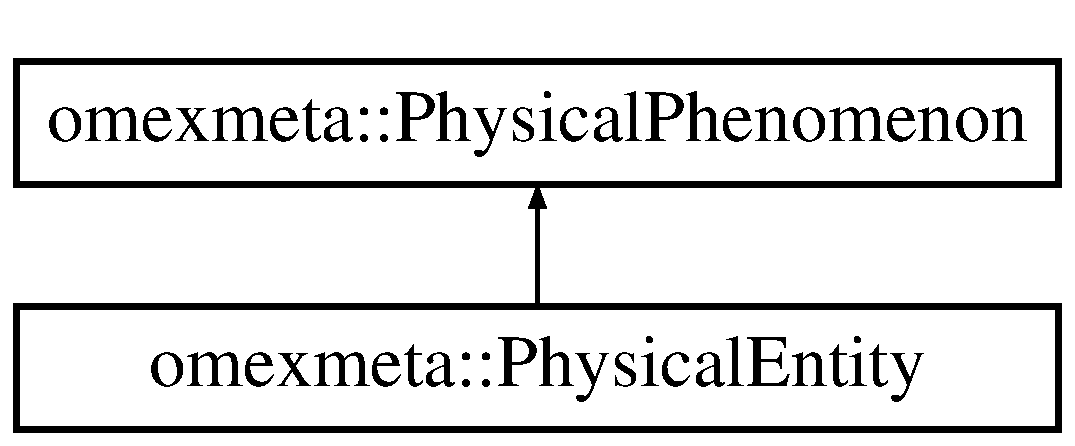
\includegraphics[height=2.000000cm]{classomexmeta_1_1PhysicalEntity}
\end{center}
\end{figure}
\subsection*{Public Member Functions}
\begin{DoxyCompactItemize}
\item 
\mbox{\Hypertarget{classomexmeta_1_1PhysicalEntity_a0341918665af91cacdb4481d037c42d2}\label{classomexmeta_1_1PhysicalEntity_a0341918665af91cacdb4481d037c42d2}} 
{\bfseries Physical\+Entity} (librdf\+\_\+model $\ast$model, std\+::string model\+\_\+uri, std\+::string local\+\_\+uri, \hyperlink{classomexmeta_1_1PhysicalProperty}{Physical\+Property} physical\+Property, \hyperlink{classomexmeta_1_1Resource}{Resource} is, Resources is\+\_\+part\+\_\+of)
\item 
\mbox{\Hypertarget{classomexmeta_1_1PhysicalEntity_a6fd4acd7255a01322c4a53d3e84df0ba}\label{classomexmeta_1_1PhysicalEntity_a6fd4acd7255a01322c4a53d3e84df0ba}} 
void {\bfseries free} ()
\item 
\mbox{\Hypertarget{classomexmeta_1_1PhysicalEntity_a6bbbce71778e374de7d4e5e2e674fc2b}\label{classomexmeta_1_1PhysicalEntity_a6bbbce71778e374de7d4e5e2e674fc2b}} 
{\bfseries Physical\+Entity} (librdf\+\_\+model $\ast$model)
\item 
\mbox{\Hypertarget{classomexmeta_1_1PhysicalEntity_a5f583e60ad44bbb3dfcd11fdc6bc72cc}\label{classomexmeta_1_1PhysicalEntity_a5f583e60ad44bbb3dfcd11fdc6bc72cc}} 
{\bfseries Physical\+Entity} (librdf\+\_\+model $\ast$model, const std\+::string \&model\+\_\+uri, const std\+::string \&local\+\_\+uri)
\item 
\mbox{\Hypertarget{classomexmeta_1_1PhysicalEntity_a51f5df8b2e8a1d65e5aa0d10e53b77ba}\label{classomexmeta_1_1PhysicalEntity_a51f5df8b2e8a1d65e5aa0d10e53b77ba}} 
\hyperlink{classomexmeta_1_1Triples}{Triples} {\bfseries to\+Triples} () override
\item 
\mbox{\Hypertarget{classomexmeta_1_1PhysicalEntity_ae4b3374e9ebb817eb63f9105b491e958}\label{classomexmeta_1_1PhysicalEntity_ae4b3374e9ebb817eb63f9105b491e958}} 
const \hyperlink{classomexmeta_1_1Resource}{Resource} \& {\bfseries get\+Identity\+Resource} () const
\item 
\mbox{\Hypertarget{classomexmeta_1_1PhysicalEntity_a3e2fba07a4622db0180650d24bf263d9}\label{classomexmeta_1_1PhysicalEntity_a3e2fba07a4622db0180650d24bf263d9}} 
const Resources \& {\bfseries get\+Location\+Resources} () const
\item 
\mbox{\Hypertarget{classomexmeta_1_1PhysicalEntity_a5d7168c527d2dbdacd612de37aa9a605}\label{classomexmeta_1_1PhysicalEntity_a5d7168c527d2dbdacd612de37aa9a605}} 
\hyperlink{classomexmeta_1_1PhysicalEntity}{Physical\+Entity} \& {\bfseries set\+Physical\+Property} (std\+::string subject\+\_\+metaid, const std\+::string \&physical\+Property)
\item 
\mbox{\Hypertarget{classomexmeta_1_1PhysicalEntity_a9bca0cb13601b6f9617df9f264968f1f}\label{classomexmeta_1_1PhysicalEntity_a9bca0cb13601b6f9617df9f264968f1f}} 
\hyperlink{classomexmeta_1_1PhysicalEntity}{Physical\+Entity} \& {\bfseries set\+Physical\+Property} (\hyperlink{classomexmeta_1_1PhysicalProperty}{Physical\+Property} physical\+Property)
\item 
\mbox{\Hypertarget{classomexmeta_1_1PhysicalEntity_a4d4c3ee9572b19e44e79a44f18f1ac31}\label{classomexmeta_1_1PhysicalEntity_a4d4c3ee9572b19e44e79a44f18f1ac31}} 
\hyperlink{classomexmeta_1_1PhysicalEntity}{Physical\+Entity} \& {\bfseries set\+Identity} (const std\+::string \&resource)
\item 
\mbox{\Hypertarget{classomexmeta_1_1PhysicalEntity_a82e77be3327c537b2426b571afaa5045}\label{classomexmeta_1_1PhysicalEntity_a82e77be3327c537b2426b571afaa5045}} 
\hyperlink{classomexmeta_1_1PhysicalEntity}{Physical\+Entity} \& {\bfseries add\+Location} (const std\+::string \&where)
\item 
\mbox{\Hypertarget{classomexmeta_1_1PhysicalEntity_a33559c90dbe3e3be1b71898ab9a5bfa4}\label{classomexmeta_1_1PhysicalEntity_a33559c90dbe3e3be1b71898ab9a5bfa4}} 
int {\bfseries get\+Num\+Locations} () const
\item 
\mbox{\Hypertarget{classomexmeta_1_1PhysicalEntity_a5f54e5c2df0fd5c3b9121e1426b23af6}\label{classomexmeta_1_1PhysicalEntity_a5f54e5c2df0fd5c3b9121e1426b23af6}} 
bool {\bfseries operator==} (const \hyperlink{classomexmeta_1_1PhysicalEntity}{Physical\+Entity} \&rhs) const
\item 
\mbox{\Hypertarget{classomexmeta_1_1PhysicalEntity_afee546a420f16e128ed1add9fec35b4f}\label{classomexmeta_1_1PhysicalEntity_afee546a420f16e128ed1add9fec35b4f}} 
bool {\bfseries operator!=} (const \hyperlink{classomexmeta_1_1PhysicalEntity}{Physical\+Entity} \&rhs) const
\end{DoxyCompactItemize}
\subsection*{Additional Inherited Members}


The documentation for this class was generated from the following files\+:\begin{DoxyCompactItemize}
\item 
src/omexmeta/Physical\+Entity.\+h\item 
src/omexmeta/Physical\+Entity.\+cpp\end{DoxyCompactItemize}

\hypertarget{classomexmeta_1_1PhysicalForce}{}\section{omexmeta\+:\+:Physical\+Force Class Reference}
\label{classomexmeta_1_1PhysicalForce}\index{omexmeta\+::\+Physical\+Force@{omexmeta\+::\+Physical\+Force}}
Inheritance diagram for omexmeta\+:\+:Physical\+Force\+:\begin{figure}[H]
\begin{center}
\leavevmode
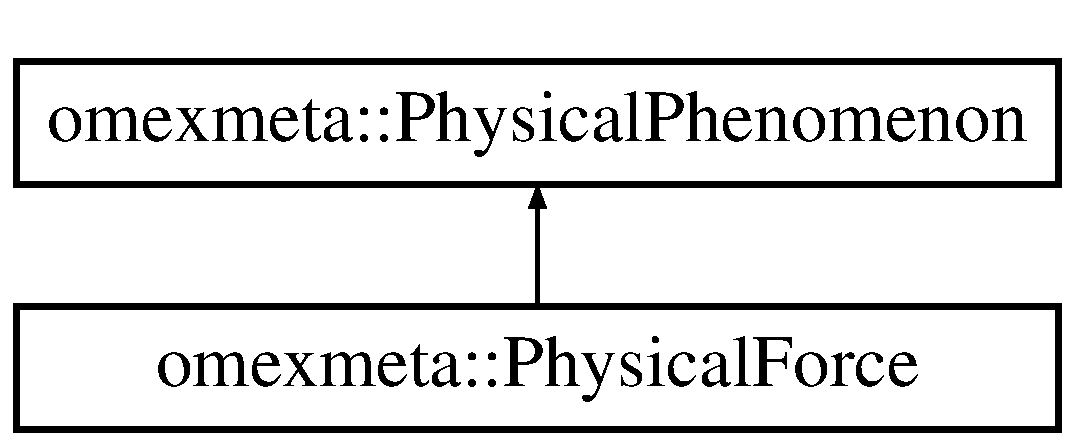
\includegraphics[height=2.000000cm]{classomexmeta_1_1PhysicalForce}
\end{center}
\end{figure}
\subsection*{Public Member Functions}
\begin{DoxyCompactItemize}
\item 
\mbox{\Hypertarget{classomexmeta_1_1PhysicalForce_a8761d703a67c6dc81b4a71b90391b20f}\label{classomexmeta_1_1PhysicalForce_a8761d703a67c6dc81b4a71b90391b20f}} 
{\bfseries Physical\+Force} (librdf\+\_\+model $\ast$model, std\+::string model\+\_\+uri, std\+::string local\+\_\+uri, \hyperlink{classomexmeta_1_1PhysicalProperty}{Physical\+Property} physical\+Property, Sources sources, Sinks sinks)
\item 
\mbox{\Hypertarget{classomexmeta_1_1PhysicalForce_a41cd6c9904f3287bb8cbbab2b9d2ada3}\label{classomexmeta_1_1PhysicalForce_a41cd6c9904f3287bb8cbbab2b9d2ada3}} 
void {\bfseries free} ()
\item 
\mbox{\Hypertarget{classomexmeta_1_1PhysicalForce_a673e6810fe969bcd087ab88c62e5e041}\label{classomexmeta_1_1PhysicalForce_a673e6810fe969bcd087ab88c62e5e041}} 
{\bfseries Physical\+Force} (librdf\+\_\+model $\ast$model)
\item 
\mbox{\Hypertarget{classomexmeta_1_1PhysicalForce_a2ff9aecd73a5356be701d8ba7e9bf71c}\label{classomexmeta_1_1PhysicalForce_a2ff9aecd73a5356be701d8ba7e9bf71c}} 
{\bfseries Physical\+Force} (librdf\+\_\+model $\ast$model, const std\+::string \&model\+\_\+uri, const std\+::string \&local\+\_\+uri)
\item 
\mbox{\Hypertarget{classomexmeta_1_1PhysicalForce_ae0a9ec4689b4765d985ab8f7a8878f38}\label{classomexmeta_1_1PhysicalForce_ae0a9ec4689b4765d985ab8f7a8878f38}} 
std\+::string {\bfseries create\+Meta\+Id} ()
\item 
\mbox{\Hypertarget{classomexmeta_1_1PhysicalForce_aa42b8e04573d2ae88f952c76b146d5ac}\label{classomexmeta_1_1PhysicalForce_aa42b8e04573d2ae88f952c76b146d5ac}} 
const Sources \& {\bfseries get\+Sources} () const
\item 
\mbox{\Hypertarget{classomexmeta_1_1PhysicalForce_ab37bbe3a0f762066fdb43e5c2ce608eb}\label{classomexmeta_1_1PhysicalForce_ab37bbe3a0f762066fdb43e5c2ce608eb}} 
const Sinks \& {\bfseries get\+Sinks} () const
\item 
\mbox{\Hypertarget{classomexmeta_1_1PhysicalForce_a39dd511aee85130d07cb6ffb3f8e87f0}\label{classomexmeta_1_1PhysicalForce_a39dd511aee85130d07cb6ffb3f8e87f0}} 
\hyperlink{classomexmeta_1_1Triples}{Triples} {\bfseries to\+Triples} () override
\item 
\mbox{\Hypertarget{classomexmeta_1_1PhysicalForce_a081aecc43d16b2fc8826c4050eb2055d}\label{classomexmeta_1_1PhysicalForce_a081aecc43d16b2fc8826c4050eb2055d}} 
\hyperlink{classomexmeta_1_1PhysicalForce}{Physical\+Force} \& {\bfseries set\+Physical\+Property} (\hyperlink{classomexmeta_1_1PhysicalProperty}{Physical\+Property} physical\+Property)
\item 
\mbox{\Hypertarget{classomexmeta_1_1PhysicalForce_a3f979432322d40efc8a15cf5ee883100}\label{classomexmeta_1_1PhysicalForce_a3f979432322d40efc8a15cf5ee883100}} 
\hyperlink{classomexmeta_1_1PhysicalForce}{Physical\+Force} \& {\bfseries set\+Physical\+Property} (std\+::string subject\+\_\+metaid, std\+::string physical\+\_\+property)
\item 
\mbox{\Hypertarget{classomexmeta_1_1PhysicalForce_ace7d3703d7e4bdb9a256208f456f2c4f}\label{classomexmeta_1_1PhysicalForce_ace7d3703d7e4bdb9a256208f456f2c4f}} 
\hyperlink{classomexmeta_1_1PhysicalForce}{Physical\+Force} \& {\bfseries add\+Source} (int multiplier, const std\+::string \&physical\+\_\+entity\+\_\+reference)
\item 
\mbox{\Hypertarget{classomexmeta_1_1PhysicalForce_a8ec5e262b82526ac914d8c7f10b6c2f1}\label{classomexmeta_1_1PhysicalForce_a8ec5e262b82526ac914d8c7f10b6c2f1}} 
\hyperlink{classomexmeta_1_1PhysicalForce}{Physical\+Force} \& {\bfseries add\+Sink} (int multiplier, const std\+::string \&physical\+\_\+entity\+\_\+reference)
\item 
\mbox{\Hypertarget{classomexmeta_1_1PhysicalForce_a9910c8edac57daf70faa1f1e2e0208d1}\label{classomexmeta_1_1PhysicalForce_a9910c8edac57daf70faa1f1e2e0208d1}} 
int {\bfseries get\+Num\+Sources} ()
\item 
\mbox{\Hypertarget{classomexmeta_1_1PhysicalForce_a1135c75705b59afa7037bab313009534}\label{classomexmeta_1_1PhysicalForce_a1135c75705b59afa7037bab313009534}} 
int {\bfseries get\+Num\+Sinks} ()
\item 
\mbox{\Hypertarget{classomexmeta_1_1PhysicalForce_affa0a1f3cdce0a3336d56658a92c65f3}\label{classomexmeta_1_1PhysicalForce_affa0a1f3cdce0a3336d56658a92c65f3}} 
bool {\bfseries operator==} (const \hyperlink{classomexmeta_1_1PhysicalForce}{Physical\+Force} \&rhs) const
\item 
\mbox{\Hypertarget{classomexmeta_1_1PhysicalForce_aeb7adb235c0caac04c7aa599f98f258a}\label{classomexmeta_1_1PhysicalForce_aeb7adb235c0caac04c7aa599f98f258a}} 
bool {\bfseries operator!=} (const \hyperlink{classomexmeta_1_1PhysicalForce}{Physical\+Force} \&rhs) const
\end{DoxyCompactItemize}
\subsection*{Additional Inherited Members}


The documentation for this class was generated from the following files\+:\begin{DoxyCompactItemize}
\item 
src/omexmeta/Physical\+Force.\+h\item 
src/omexmeta/Physical\+Force.\+cpp\end{DoxyCompactItemize}

\hypertarget{classomexmeta_1_1PhysicalPhenomenon}{}\section{omexmeta\+:\+:Physical\+Phenomenon Class Reference}
\label{classomexmeta_1_1PhysicalPhenomenon}\index{omexmeta\+::\+Physical\+Phenomenon@{omexmeta\+::\+Physical\+Phenomenon}}
Inheritance diagram for omexmeta\+:\+:Physical\+Phenomenon\+:\begin{figure}[H]
\begin{center}
\leavevmode
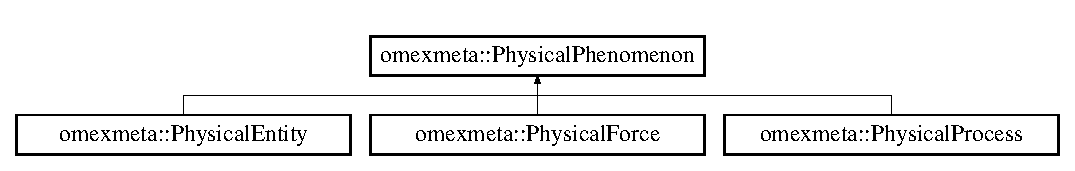
\includegraphics[height=1.848185cm]{classomexmeta_1_1PhysicalPhenomenon}
\end{center}
\end{figure}
\subsection*{Public Member Functions}
\begin{DoxyCompactItemize}
\item 
\mbox{\Hypertarget{classomexmeta_1_1PhysicalPhenomenon_a1c3322453b3c6831668ffa98d9f4b6af}\label{classomexmeta_1_1PhysicalPhenomenon_a1c3322453b3c6831668ffa98d9f4b6af}} 
bool {\bfseries operator==} (const \hyperlink{classomexmeta_1_1PhysicalPhenomenon}{Physical\+Phenomenon} \&rhs) const
\item 
\mbox{\Hypertarget{classomexmeta_1_1PhysicalPhenomenon_a2c726263714e31c7c19d6e73c2c593f8}\label{classomexmeta_1_1PhysicalPhenomenon_a2c726263714e31c7c19d6e73c2c593f8}} 
bool {\bfseries operator!=} (const \hyperlink{classomexmeta_1_1PhysicalPhenomenon}{Physical\+Phenomenon} \&rhs) const
\item 
\mbox{\Hypertarget{classomexmeta_1_1PhysicalPhenomenon_a2d59ebbc920a40348d102af31ed6661a}\label{classomexmeta_1_1PhysicalPhenomenon_a2d59ebbc920a40348d102af31ed6661a}} 
const std\+::string \& {\bfseries get\+Local\+Uri} () const
\item 
\mbox{\Hypertarget{classomexmeta_1_1PhysicalPhenomenon_a84cae9aa96ca00df45b0f81dd8d3ffd4}\label{classomexmeta_1_1PhysicalPhenomenon_a84cae9aa96ca00df45b0f81dd8d3ffd4}} 
void {\bfseries set\+Local\+Uri} (const std\+::string \&local\+Uri)
\item 
\mbox{\Hypertarget{classomexmeta_1_1PhysicalPhenomenon_ad823dad75504adb78975c810e5f1ff94}\label{classomexmeta_1_1PhysicalPhenomenon_ad823dad75504adb78975c810e5f1ff94}} 
{\bfseries Physical\+Phenomenon} (const \hyperlink{classomexmeta_1_1PhysicalPhenomenon}{Physical\+Phenomenon} \&phenomenon)=delete
\item 
\mbox{\Hypertarget{classomexmeta_1_1PhysicalPhenomenon_aeb95aedf1756ded154ec6753108a691e}\label{classomexmeta_1_1PhysicalPhenomenon_aeb95aedf1756ded154ec6753108a691e}} 
{\bfseries Physical\+Phenomenon} (\hyperlink{classomexmeta_1_1PhysicalPhenomenon}{Physical\+Phenomenon} \&\&phenomenon) noexcept
\item 
\mbox{\Hypertarget{classomexmeta_1_1PhysicalPhenomenon_aac3920bfe9bf16e071ebdd8ed4fabe2f}\label{classomexmeta_1_1PhysicalPhenomenon_aac3920bfe9bf16e071ebdd8ed4fabe2f}} 
\hyperlink{classomexmeta_1_1PhysicalPhenomenon}{Physical\+Phenomenon} \& {\bfseries operator=} (const \hyperlink{classomexmeta_1_1PhysicalPhenomenon}{Physical\+Phenomenon} \&phenomenon)=delete
\item 
\mbox{\Hypertarget{classomexmeta_1_1PhysicalPhenomenon_af15355b4c2a361b4b02dca02d3877aed}\label{classomexmeta_1_1PhysicalPhenomenon_af15355b4c2a361b4b02dca02d3877aed}} 
\hyperlink{classomexmeta_1_1PhysicalPhenomenon}{Physical\+Phenomenon} \& {\bfseries operator=} (\hyperlink{classomexmeta_1_1PhysicalPhenomenon}{Physical\+Phenomenon} \&\&phenomenon) noexcept
\item 
\mbox{\Hypertarget{classomexmeta_1_1PhysicalPhenomenon_aa140516da97b03960175f9bc04ecf865}\label{classomexmeta_1_1PhysicalPhenomenon_aa140516da97b03960175f9bc04ecf865}} 
{\bfseries Physical\+Phenomenon} (librdf\+\_\+model $\ast$model)
\item 
\mbox{\Hypertarget{classomexmeta_1_1PhysicalPhenomenon_a5c831ca76c36121b0fbc7b122b5539ac}\label{classomexmeta_1_1PhysicalPhenomenon_a5c831ca76c36121b0fbc7b122b5539ac}} 
{\bfseries Physical\+Phenomenon} (librdf\+\_\+model $\ast$model, std\+::string model\+\_\+uri, std\+::string local\+\_\+uri)
\item 
\mbox{\Hypertarget{classomexmeta_1_1PhysicalPhenomenon_a93bf263f7fdb65bd3e8de97983a7186b}\label{classomexmeta_1_1PhysicalPhenomenon_a93bf263f7fdb65bd3e8de97983a7186b}} 
{\bfseries Physical\+Phenomenon} (librdf\+\_\+model $\ast$model, std\+::string model\+\_\+uri, std\+::string local\+\_\+uri, \hyperlink{classomexmeta_1_1PhysicalProperty}{Physical\+Property} property\+Resource, Annotation\+Type type)
\item 
\mbox{\Hypertarget{classomexmeta_1_1PhysicalPhenomenon_a5528b12e5dbc702c0c270328662e7031}\label{classomexmeta_1_1PhysicalPhenomenon_a5528b12e5dbc702c0c270328662e7031}} 
const std\+::string \& {\bfseries get\+Model\+Uri} () const
\item 
\mbox{\Hypertarget{classomexmeta_1_1PhysicalPhenomenon_aa1fd9929fb2e07fa20081b1a4c00c9d2}\label{classomexmeta_1_1PhysicalPhenomenon_aa1fd9929fb2e07fa20081b1a4c00c9d2}} 
void {\bfseries set\+Model\+Uri} (const std\+::string \&model\+Uri)
\item 
\mbox{\Hypertarget{classomexmeta_1_1PhysicalPhenomenon_a8be912d1256d6b913c4965f96f1b730b}\label{classomexmeta_1_1PhysicalPhenomenon_a8be912d1256d6b913c4965f96f1b730b}} 
const std\+::string \& {\bfseries get\+About} () const
\item 
\mbox{\Hypertarget{classomexmeta_1_1PhysicalPhenomenon_a9676a1dcc458247a19d19cda16d640f4}\label{classomexmeta_1_1PhysicalPhenomenon_a9676a1dcc458247a19d19cda16d640f4}} 
Annotation\+Type {\bfseries get\+Type} () const
\item 
\mbox{\Hypertarget{classomexmeta_1_1PhysicalPhenomenon_ac741cab1f6df58b0de484fc1771ef839}\label{classomexmeta_1_1PhysicalPhenomenon_ac741cab1f6df58b0de484fc1771ef839}} 
\hyperlink{classomexmeta_1_1PhysicalProperty}{Physical\+Property} {\bfseries get\+Physical\+Property} () const
\item 
\mbox{\Hypertarget{classomexmeta_1_1PhysicalPhenomenon_a30617e685bd8b155a76d38ab5a9db273}\label{classomexmeta_1_1PhysicalPhenomenon_a30617e685bd8b155a76d38ab5a9db273}} 
virtual \hyperlink{classomexmeta_1_1Triples}{Triples} {\bfseries to\+Triples} ()
\item 
\mbox{\Hypertarget{classomexmeta_1_1PhysicalPhenomenon_ae99e667cbceff2da0c4c0f5c64a8ba8f}\label{classomexmeta_1_1PhysicalPhenomenon_ae99e667cbceff2da0c4c0f5c64a8ba8f}} 
const std\+::string \& {\bfseries get\+Subject\+Str} () const
\item 
\mbox{\Hypertarget{classomexmeta_1_1PhysicalPhenomenon_a0a9c54b0c4bfad62b618766474dc70f8}\label{classomexmeta_1_1PhysicalPhenomenon_a0a9c54b0c4bfad62b618766474dc70f8}} 
\hyperlink{classomexmeta_1_1PhysicalPhenomenon}{Physical\+Phenomenon} \& {\bfseries set\+About} (std\+::string about)
\item 
\mbox{\Hypertarget{classomexmeta_1_1PhysicalPhenomenon_afad41dbf096b22ab9b64441cb25e9db9}\label{classomexmeta_1_1PhysicalPhenomenon_afad41dbf096b22ab9b64441cb25e9db9}} 
void {\bfseries set\+Physical\+Property} (const \hyperlink{classomexmeta_1_1PhysicalProperty}{Physical\+Property} \&physical\+Property)
\item 
\mbox{\Hypertarget{classomexmeta_1_1PhysicalPhenomenon_a4c27a0b0e430df95b3cffaf268973eec}\label{classomexmeta_1_1PhysicalPhenomenon_a4c27a0b0e430df95b3cffaf268973eec}} 
void {\bfseries set\+Type} (Annotation\+Type type)
\item 
\mbox{\Hypertarget{classomexmeta_1_1PhysicalPhenomenon_aca53e0f8ce8139a919f48372b254a5d0}\label{classomexmeta_1_1PhysicalPhenomenon_aca53e0f8ce8139a919f48372b254a5d0}} 
const std\+::string \& {\bfseries get\+Physical\+Property\+Id} () const
\item 
\mbox{\Hypertarget{classomexmeta_1_1PhysicalPhenomenon_a715b76003eba8e5808fe44a768199fab}\label{classomexmeta_1_1PhysicalPhenomenon_a715b76003eba8e5808fe44a768199fab}} 
void {\bfseries set\+Physical\+Property\+Id} (const std\+::string \&physical\+Property\+Id)
\end{DoxyCompactItemize}
\subsection*{Protected Member Functions}
\begin{DoxyCompactItemize}
\item 
\mbox{\Hypertarget{classomexmeta_1_1PhysicalPhenomenon_a54d90cf6db78e98bd091f478dc5bd74a}\label{classomexmeta_1_1PhysicalPhenomenon_a54d90cf6db78e98bd091f478dc5bd74a}} 
std\+::vector$<$ std\+::string $>$ {\bfseries get\+New\+Metaid\+Exclusion\+List} ()
\item 
\mbox{\Hypertarget{classomexmeta_1_1PhysicalPhenomenon_afe71a5c6399b992922eb6eeda6de49bd}\label{classomexmeta_1_1PhysicalPhenomenon_afe71a5c6399b992922eb6eeda6de49bd}} 
std\+::string {\bfseries generate\+Meta\+Id} (const std\+::string \&id\+\_\+base)
\end{DoxyCompactItemize}
\subsection*{Protected Attributes}
\begin{DoxyCompactItemize}
\item 
\mbox{\Hypertarget{classomexmeta_1_1PhysicalPhenomenon_a9de43fc3fd94d3463c7fb9b8f684e78b}\label{classomexmeta_1_1PhysicalPhenomenon_a9de43fc3fd94d3463c7fb9b8f684e78b}} 
librdf\+\_\+model $\ast$ {\bfseries model\+\_\+} = nullptr
\item 
\mbox{\Hypertarget{classomexmeta_1_1PhysicalPhenomenon_a9e17807d60d9e3f797d6c02ef85cdfc6}\label{classomexmeta_1_1PhysicalPhenomenon_a9e17807d60d9e3f797d6c02ef85cdfc6}} 
\hyperlink{classomexmeta_1_1PhysicalProperty}{Physical\+Property} {\bfseries physical\+\_\+property\+\_\+}
\item 
\mbox{\Hypertarget{classomexmeta_1_1PhysicalPhenomenon_a74e88adb2099099e411b55cb9aa460a0}\label{classomexmeta_1_1PhysicalPhenomenon_a74e88adb2099099e411b55cb9aa460a0}} 
Annotation\+Type {\bfseries type\+\_\+} = Annotation\+Type\+::\+U\+N\+K\+N\+O\+WN
\item 
\mbox{\Hypertarget{classomexmeta_1_1PhysicalPhenomenon_a696cbc4f6490dd55d6bd41c7711cd0ec}\label{classomexmeta_1_1PhysicalPhenomenon_a696cbc4f6490dd55d6bd41c7711cd0ec}} 
std\+::string {\bfseries model\+\_\+uri\+\_\+}
\item 
\mbox{\Hypertarget{classomexmeta_1_1PhysicalPhenomenon_a114864dfae1f79ce4e3f430b7711516c}\label{classomexmeta_1_1PhysicalPhenomenon_a114864dfae1f79ce4e3f430b7711516c}} 
std\+::string {\bfseries local\+\_\+uri\+\_\+}
\item 
\mbox{\Hypertarget{classomexmeta_1_1PhysicalPhenomenon_a710756d611350395539dfa9f7fbf764e}\label{classomexmeta_1_1PhysicalPhenomenon_a710756d611350395539dfa9f7fbf764e}} 
std\+::vector$<$ std\+::string $>$ {\bfseries new\+\_\+metaid\+\_\+exclusion\+\_\+list\+\_\+}
\end{DoxyCompactItemize}


The documentation for this class was generated from the following files\+:\begin{DoxyCompactItemize}
\item 
src/omexmeta/Physical\+Phenomenon.\+h\item 
src/omexmeta/Physical\+Phenomenon.\+cpp\end{DoxyCompactItemize}

\hypertarget{classomexmeta_1_1PhysicalProcess}{}\section{omexmeta\+:\+:Physical\+Process Class Reference}
\label{classomexmeta_1_1PhysicalProcess}\index{omexmeta\+::\+Physical\+Process@{omexmeta\+::\+Physical\+Process}}
Inheritance diagram for omexmeta\+:\+:Physical\+Process\+:\begin{figure}[H]
\begin{center}
\leavevmode
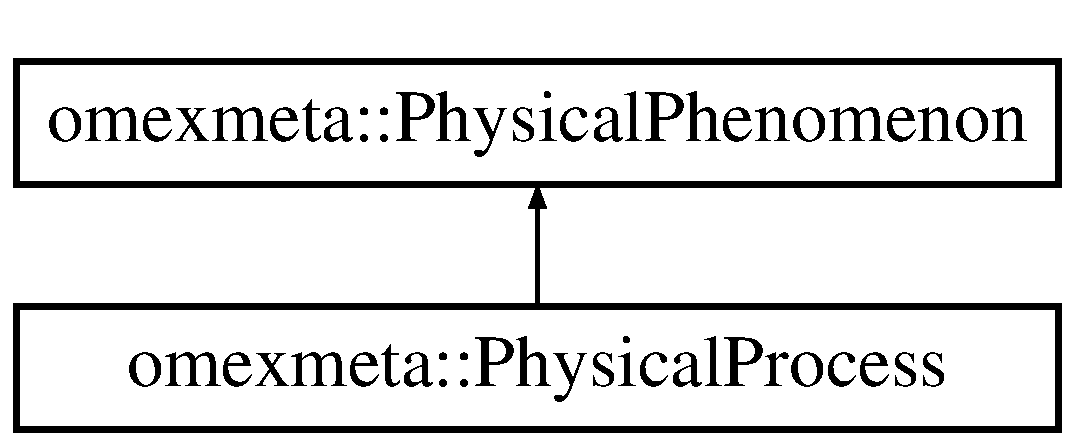
\includegraphics[height=2.000000cm]{classomexmeta_1_1PhysicalProcess}
\end{center}
\end{figure}
\subsection*{Public Member Functions}
\begin{DoxyCompactItemize}
\item 
\mbox{\Hypertarget{classomexmeta_1_1PhysicalProcess_a37f99033da4635ff1af2b9f19c1b84ce}\label{classomexmeta_1_1PhysicalProcess_a37f99033da4635ff1af2b9f19c1b84ce}} 
{\bfseries Physical\+Process} (librdf\+\_\+model $\ast$model, std\+::string model\+\_\+uri, std\+::string local\+\_\+uri, const \hyperlink{classomexmeta_1_1PhysicalProperty}{Physical\+Property} \&physical\+Property, Sources sources, Sinks sinks, Mediators mediators)
\item 
\mbox{\Hypertarget{classomexmeta_1_1PhysicalProcess_a8dfcffe80f264ad24e70de9d7b71c73b}\label{classomexmeta_1_1PhysicalProcess_a8dfcffe80f264ad24e70de9d7b71c73b}} 
void {\bfseries free} ()
\item 
\mbox{\Hypertarget{classomexmeta_1_1PhysicalProcess_a2b694395a318335e81c884ed76b5f4dd}\label{classomexmeta_1_1PhysicalProcess_a2b694395a318335e81c884ed76b5f4dd}} 
{\bfseries Physical\+Process} (librdf\+\_\+model $\ast$model)
\item 
\mbox{\Hypertarget{classomexmeta_1_1PhysicalProcess_a974e2717dbf4b690b95b07e9c026fd2a}\label{classomexmeta_1_1PhysicalProcess_a974e2717dbf4b690b95b07e9c026fd2a}} 
{\bfseries Physical\+Process} (librdf\+\_\+model $\ast$model, std\+::string model\+\_\+uri, std\+::string local\+\_\+uri)
\item 
\mbox{\Hypertarget{classomexmeta_1_1PhysicalProcess_ab5f3100febc21173775a2090bb57a0fb}\label{classomexmeta_1_1PhysicalProcess_ab5f3100febc21173775a2090bb57a0fb}} 
const Sources \& {\bfseries get\+Sources} () const
\item 
\mbox{\Hypertarget{classomexmeta_1_1PhysicalProcess_a069e7caa05f346f90f413f650f081535}\label{classomexmeta_1_1PhysicalProcess_a069e7caa05f346f90f413f650f081535}} 
const Sinks \& {\bfseries get\+Sinks} () const
\item 
\mbox{\Hypertarget{classomexmeta_1_1PhysicalProcess_a349b76ad1831d2510904510583f0d7f2}\label{classomexmeta_1_1PhysicalProcess_a349b76ad1831d2510904510583f0d7f2}} 
const Mediators \& {\bfseries get\+Mediators} () const
\item 
\mbox{\Hypertarget{classomexmeta_1_1PhysicalProcess_ab6f6af00fac2401f9a88e186fd1d897a}\label{classomexmeta_1_1PhysicalProcess_ab6f6af00fac2401f9a88e186fd1d897a}} 
\hyperlink{classomexmeta_1_1Triples}{Triples} {\bfseries to\+Triples} () override
\item 
\mbox{\Hypertarget{classomexmeta_1_1PhysicalProcess_ac875058d67408246aa28cf58dd77ccf6}\label{classomexmeta_1_1PhysicalProcess_ac875058d67408246aa28cf58dd77ccf6}} 
\hyperlink{classomexmeta_1_1PhysicalProcess}{Physical\+Process} \& {\bfseries set\+Physical\+Property} (std\+::string subject\+\_\+metaid, const std\+::string \&physical\+Property)
\item 
\mbox{\Hypertarget{classomexmeta_1_1PhysicalProcess_ac49bf4a1c21c6590a9d2af7ae93e13a7}\label{classomexmeta_1_1PhysicalProcess_ac49bf4a1c21c6590a9d2af7ae93e13a7}} 
\hyperlink{classomexmeta_1_1PhysicalProcess}{Physical\+Process} \& {\bfseries set\+Physical\+Property} (\hyperlink{classomexmeta_1_1PhysicalProperty}{Physical\+Property} physical\+Property)
\item 
\mbox{\Hypertarget{classomexmeta_1_1PhysicalProcess_ab83f58b7df77fdee131c22c71da22f39}\label{classomexmeta_1_1PhysicalProcess_ab83f58b7df77fdee131c22c71da22f39}} 
\hyperlink{classomexmeta_1_1PhysicalProcess}{Physical\+Process} \& {\bfseries add\+Source} (int multiplier, std\+::string physical\+\_\+entity\+\_\+reference)
\item 
\mbox{\Hypertarget{classomexmeta_1_1PhysicalProcess_a403ffc7d7d29702f2ff4e56084a1d714}\label{classomexmeta_1_1PhysicalProcess_a403ffc7d7d29702f2ff4e56084a1d714}} 
\hyperlink{classomexmeta_1_1PhysicalProcess}{Physical\+Process} \& {\bfseries add\+Sink} (int multiplier, std\+::string physical\+\_\+entity\+\_\+reference)
\item 
\mbox{\Hypertarget{classomexmeta_1_1PhysicalProcess_a2bdf8dde5ffa6b38d5042db49fd211d1}\label{classomexmeta_1_1PhysicalProcess_a2bdf8dde5ffa6b38d5042db49fd211d1}} 
\hyperlink{classomexmeta_1_1PhysicalProcess}{Physical\+Process} \& {\bfseries add\+Mediator} (std\+::string physical\+\_\+entity\+\_\+reference)
\item 
\mbox{\Hypertarget{classomexmeta_1_1PhysicalProcess_a56459d9f0087a3f92b0aca5d148b65f5}\label{classomexmeta_1_1PhysicalProcess_a56459d9f0087a3f92b0aca5d148b65f5}} 
int {\bfseries get\+Num\+Sources} ()
\item 
\mbox{\Hypertarget{classomexmeta_1_1PhysicalProcess_ac8b79af15d4d19042ee34abca25f679f}\label{classomexmeta_1_1PhysicalProcess_ac8b79af15d4d19042ee34abca25f679f}} 
int {\bfseries get\+Num\+Sinks} ()
\item 
\mbox{\Hypertarget{classomexmeta_1_1PhysicalProcess_a717a352ce3bb956201174002f904cd26}\label{classomexmeta_1_1PhysicalProcess_a717a352ce3bb956201174002f904cd26}} 
int {\bfseries get\+Num\+Mediators} ()
\item 
\mbox{\Hypertarget{classomexmeta_1_1PhysicalProcess_a65585bf5cd473d509f6f66c96757ff8d}\label{classomexmeta_1_1PhysicalProcess_a65585bf5cd473d509f6f66c96757ff8d}} 
bool {\bfseries operator==} (const \hyperlink{classomexmeta_1_1PhysicalProcess}{Physical\+Process} \&rhs) const
\item 
\mbox{\Hypertarget{classomexmeta_1_1PhysicalProcess_af8298394b713807ec51c2b5f60afd00e}\label{classomexmeta_1_1PhysicalProcess_af8298394b713807ec51c2b5f60afd00e}} 
bool {\bfseries operator!=} (const \hyperlink{classomexmeta_1_1PhysicalProcess}{Physical\+Process} \&rhs) const
\end{DoxyCompactItemize}
\subsection*{Additional Inherited Members}


The documentation for this class was generated from the following files\+:\begin{DoxyCompactItemize}
\item 
src/omexmeta/Physical\+Process.\+h\item 
src/omexmeta/Physical\+Process.\+cpp\end{DoxyCompactItemize}

\hypertarget{classomexmeta_1_1PhysicalProperty}{}\section{omexmeta\+:\+:Physical\+Property Class Reference}
\label{classomexmeta_1_1PhysicalProperty}\index{omexmeta\+::\+Physical\+Property@{omexmeta\+::\+Physical\+Property}}
\subsection*{Public Member Functions}
\begin{DoxyCompactItemize}
\item 
\mbox{\Hypertarget{classomexmeta_1_1PhysicalProperty_af3b3379a751ebb15f7a5ea0cae8cb4d6}\label{classomexmeta_1_1PhysicalProperty_af3b3379a751ebb15f7a5ea0cae8cb4d6}} 
bool {\bfseries operator==} (const \hyperlink{classomexmeta_1_1PhysicalProperty}{Physical\+Property} \&rhs) const
\item 
\mbox{\Hypertarget{classomexmeta_1_1PhysicalProperty_a1a85ba2c50f5b79e49e8a01b96756f0a}\label{classomexmeta_1_1PhysicalProperty_a1a85ba2c50f5b79e49e8a01b96756f0a}} 
bool {\bfseries operator!=} (const \hyperlink{classomexmeta_1_1PhysicalProperty}{Physical\+Property} \&rhs) const
\item 
\mbox{\Hypertarget{classomexmeta_1_1PhysicalProperty_a76d1ffd15ea6aad76c322bdd8991a111}\label{classomexmeta_1_1PhysicalProperty_a76d1ffd15ea6aad76c322bdd8991a111}} 
{\bfseries Physical\+Property} (std\+::string subject\+\_\+str, std\+::string resource\+\_\+str, std\+::string model\+\_\+uri)
\item 
\mbox{\Hypertarget{classomexmeta_1_1PhysicalProperty_acf399e14fd579efc6384ebc677341ead}\label{classomexmeta_1_1PhysicalProperty_acf399e14fd579efc6384ebc677341ead}} 
const std\+::string \& {\bfseries get\+Subject} () const
\item 
\mbox{\Hypertarget{classomexmeta_1_1PhysicalProperty_a2d60b90270a6ba73646707b8c475fbb1}\label{classomexmeta_1_1PhysicalProperty_a2d60b90270a6ba73646707b8c475fbb1}} 
const std\+::string \& {\bfseries get\+Resource} () const
\item 
\mbox{\Hypertarget{classomexmeta_1_1PhysicalProperty_a0f27071bfef5a9de4eb89fb21461ba76}\label{classomexmeta_1_1PhysicalProperty_a0f27071bfef5a9de4eb89fb21461ba76}} 
const std\+::string \& {\bfseries get\+Model\+Uri} () const
\item 
\mbox{\Hypertarget{classomexmeta_1_1PhysicalProperty_afd367b237fc93654c59c3b0c203b4640}\label{classomexmeta_1_1PhysicalProperty_afd367b237fc93654c59c3b0c203b4640}} 
void {\bfseries set\+Model\+Uri} (const std\+::string \&model\+\_\+uri)
\item 
\mbox{\Hypertarget{classomexmeta_1_1PhysicalProperty_a4b9ad0a7fe22a3476d7e2f08834bbd74}\label{classomexmeta_1_1PhysicalProperty_a4b9ad0a7fe22a3476d7e2f08834bbd74}} 
const std\+::string \& {\bfseries get\+Subject\+Str} () const
\item 
\mbox{\Hypertarget{classomexmeta_1_1PhysicalProperty_a8bb7c912a21e0e318a9e16d2af1801e5}\label{classomexmeta_1_1PhysicalProperty_a8bb7c912a21e0e318a9e16d2af1801e5}} 
void {\bfseries set\+Subject} (const std\+::string \&subject)
\item 
\mbox{\Hypertarget{classomexmeta_1_1PhysicalProperty_a9177d21e829cbd872217ba6f9619d427}\label{classomexmeta_1_1PhysicalProperty_a9177d21e829cbd872217ba6f9619d427}} 
const std\+::string \& {\bfseries get\+Resource\+Str} () const
\item 
\mbox{\Hypertarget{classomexmeta_1_1PhysicalProperty_a420dab52a424d1be5a8610e19407980c}\label{classomexmeta_1_1PhysicalProperty_a420dab52a424d1be5a8610e19407980c}} 
void {\bfseries set\+Resource} (const std\+::string \&resource)
\item 
\mbox{\Hypertarget{classomexmeta_1_1PhysicalProperty_a03056210a70ea8446b44de250646eeb5}\label{classomexmeta_1_1PhysicalProperty_a03056210a70ea8446b44de250646eeb5}} 
\hyperlink{classomexmeta_1_1Triples}{Triples} {\bfseries to\+Triples} (const std\+::string \&property\+\_\+metaid) const
\end{DoxyCompactItemize}


The documentation for this class was generated from the following files\+:\begin{DoxyCompactItemize}
\item 
src/omexmeta/Physical\+Property.\+h\item 
src/omexmeta/Physical\+Property.\+cpp\end{DoxyCompactItemize}

\hypertarget{classomexmeta_1_1Predicate}{}\section{omexmeta\+:\+:Predicate Class Reference}
\label{classomexmeta_1_1Predicate}\index{omexmeta\+::\+Predicate@{omexmeta\+::\+Predicate}}
Inheritance diagram for omexmeta\+:\+:Predicate\+:\begin{figure}[H]
\begin{center}
\leavevmode
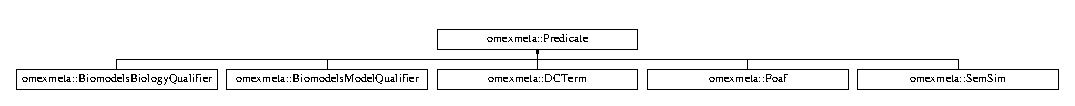
\includegraphics[height=0.978166cm]{classomexmeta_1_1Predicate}
\end{center}
\end{figure}
\subsection*{Public Member Functions}
\begin{DoxyCompactItemize}
\item 
\mbox{\Hypertarget{classomexmeta_1_1Predicate_ad5a91eb29204202d2f18816d09677622}\label{classomexmeta_1_1Predicate_ad5a91eb29204202d2f18816d09677622}} 
{\bfseries Predicate} (const std\+::string \&namespace\+\_\+, std\+::string term, std\+::string prefix)
\item 
\mbox{\Hypertarget{classomexmeta_1_1Predicate_a5db1e6150f8cfd7605e82996e2aebb50}\label{classomexmeta_1_1Predicate_a5db1e6150f8cfd7605e82996e2aebb50}} 
bool {\bfseries operator==} (const \hyperlink{classomexmeta_1_1Predicate}{Predicate} \&rhs) const
\item 
\mbox{\Hypertarget{classomexmeta_1_1Predicate_a7bf4b8769eb9801eb26cc976723b56f2}\label{classomexmeta_1_1Predicate_a7bf4b8769eb9801eb26cc976723b56f2}} 
bool {\bfseries operator!=} (const \hyperlink{classomexmeta_1_1Predicate}{Predicate} \&rhs) const
\item 
\mbox{\Hypertarget{classomexmeta_1_1Predicate_a9d51ebf565f39fb4d6d4f58c1b030edf}\label{classomexmeta_1_1Predicate_a9d51ebf565f39fb4d6d4f58c1b030edf}} 
std\+::string {\bfseries str} ()
\item 
\mbox{\Hypertarget{classomexmeta_1_1Predicate_a144efc75a923b9d85b9f8eaccf0400bb}\label{classomexmeta_1_1Predicate_a144efc75a923b9d85b9f8eaccf0400bb}} 
librdf\+\_\+node $\ast$ {\bfseries get\+Node} () const
\item 
\mbox{\Hypertarget{classomexmeta_1_1Predicate_aee19b8fc8b21f8e5ffd5b64691e1e530}\label{classomexmeta_1_1Predicate_aee19b8fc8b21f8e5ffd5b64691e1e530}} 
const std\+::vector$<$ std\+::string $>$ \& {\bfseries get\+Valid\+Terms} () const
\item 
\mbox{\Hypertarget{classomexmeta_1_1Predicate_add4ab1cd86f83de3512279bbfdad947c}\label{classomexmeta_1_1Predicate_add4ab1cd86f83de3512279bbfdad947c}} 
const std\+::string \& {\bfseries get\+Namespace} () const
\item 
\mbox{\Hypertarget{classomexmeta_1_1Predicate_a54a15176bd697d37d00573bf86954630}\label{classomexmeta_1_1Predicate_a54a15176bd697d37d00573bf86954630}} 
const std\+::string \& {\bfseries get\+Term} () const
\item 
\mbox{\Hypertarget{classomexmeta_1_1Predicate_a0147e977f71604db05763815ae6b553f}\label{classomexmeta_1_1Predicate_a0147e977f71604db05763815ae6b553f}} 
const std\+::string \& {\bfseries get\+Prefix} () const
\item 
\mbox{\Hypertarget{classomexmeta_1_1Predicate_a27fa7d62ad9a5182f3dd642bc61c8d9f}\label{classomexmeta_1_1Predicate_a27fa7d62ad9a5182f3dd642bc61c8d9f}} 
const std\+::string \& {\bfseries get\+Uri} () const
\item 
\mbox{\Hypertarget{classomexmeta_1_1Predicate_a718a37ff90ac0f2d7cc129e8351a2c7b}\label{classomexmeta_1_1Predicate_a718a37ff90ac0f2d7cc129e8351a2c7b}} 
void {\bfseries free\+Node} ()
\item 
\mbox{\Hypertarget{classomexmeta_1_1Predicate_a0bf6030510247a6999d81cada92c1e51}\label{classomexmeta_1_1Predicate_a0bf6030510247a6999d81cada92c1e51}} 
void {\bfseries set\+Node} (librdf\+\_\+node $\ast$node)
\end{DoxyCompactItemize}
\subsection*{Static Public Member Functions}
\begin{DoxyCompactItemize}
\item 
\mbox{\Hypertarget{classomexmeta_1_1Predicate_a1291e3cd9727871f568e864e0f5af3f0}\label{classomexmeta_1_1Predicate_a1291e3cd9727871f568e864e0f5af3f0}} 
static std\+::unordered\+\_\+map$<$ std\+::string, std\+::string $>$ {\bfseries namespace\+Map} ()
\item 
\mbox{\Hypertarget{classomexmeta_1_1Predicate_a1e7e59b8a48c9f89eeec73f3bbaea19c}\label{classomexmeta_1_1Predicate_a1e7e59b8a48c9f89eeec73f3bbaea19c}} 
static void {\bfseries verify} (std\+::vector$<$ std\+::string $>$ valid\+\_\+terms, const std\+::string \&term)
\item 
\mbox{\Hypertarget{classomexmeta_1_1Predicate_a8381c8b0c7bbaa27de29608cbff08bf5}\label{classomexmeta_1_1Predicate_a8381c8b0c7bbaa27de29608cbff08bf5}} 
static bool {\bfseries namespace\+Known} (const std\+::string \&ns)
\item 
\mbox{\Hypertarget{classomexmeta_1_1Predicate_a4cda551beb4e1354ac56d692f0eb78cd}\label{classomexmeta_1_1Predicate_a4cda551beb4e1354ac56d692f0eb78cd}} 
static void {\bfseries add\+Seen\+Namespace\+To\+Serializer} (librdf\+\_\+world $\ast$world, librdf\+\_\+serializer $\ast$serializer, librdf\+\_\+node $\ast$predicate)
\end{DoxyCompactItemize}
\subsection*{Protected Member Functions}
\begin{DoxyCompactItemize}
\item 
\mbox{\Hypertarget{classomexmeta_1_1Predicate_a157c4e95f9869d4f22cd07332ff7621a}\label{classomexmeta_1_1Predicate_a157c4e95f9869d4f22cd07332ff7621a}} 
{\bfseries Predicate} (librdf\+\_\+node $\ast$node)
\end{DoxyCompactItemize}
\subsection*{Protected Attributes}
\begin{DoxyCompactItemize}
\item 
\mbox{\Hypertarget{classomexmeta_1_1Predicate_afc79b0cc43eb11e4bc2fe0b305e551bc}\label{classomexmeta_1_1Predicate_afc79b0cc43eb11e4bc2fe0b305e551bc}} 
std\+::string {\bfseries namespace\+\_\+}
\item 
\mbox{\Hypertarget{classomexmeta_1_1Predicate_ab626a5fd9fa8f302767d4ca544a9eff2}\label{classomexmeta_1_1Predicate_ab626a5fd9fa8f302767d4ca544a9eff2}} 
std\+::string {\bfseries term\+\_\+}
\item 
\mbox{\Hypertarget{classomexmeta_1_1Predicate_a5dfbbc85f7bdc5a3e4da72913f6ce306}\label{classomexmeta_1_1Predicate_a5dfbbc85f7bdc5a3e4da72913f6ce306}} 
std\+::string {\bfseries prefix\+\_\+}
\item 
\mbox{\Hypertarget{classomexmeta_1_1Predicate_a4fe359b93a9dea9b60f7bc28c1aa913b}\label{classomexmeta_1_1Predicate_a4fe359b93a9dea9b60f7bc28c1aa913b}} 
std\+::string {\bfseries uri\+\_\+}
\item 
\mbox{\Hypertarget{classomexmeta_1_1Predicate_ad0548a6d31dbc6f32734032b1540e58f}\label{classomexmeta_1_1Predicate_ad0548a6d31dbc6f32734032b1540e58f}} 
librdf\+\_\+node $\ast$ {\bfseries node\+\_\+} = nullptr
\item 
\mbox{\Hypertarget{classomexmeta_1_1Predicate_a14ae7768fbd3aaf444bcde8650910c0b}\label{classomexmeta_1_1Predicate_a14ae7768fbd3aaf444bcde8650910c0b}} 
std\+::vector$<$ std\+::string $>$ \hyperlink{classomexmeta_1_1Predicate_a14ae7768fbd3aaf444bcde8650910c0b}{valid\+\_\+terms\+\_\+} \{\char`\"{}All\char`\"{}\}
\begin{DoxyCompactList}\small\item\em predicates can only have type uri \end{DoxyCompactList}\end{DoxyCompactItemize}


The documentation for this class was generated from the following files\+:\begin{DoxyCompactItemize}
\item 
src/omexmeta/Predicate.\+h\item 
src/omexmeta/Predicate.\+cpp\end{DoxyCompactItemize}

\hypertarget{structdbg_1_1pretty__print__tuple}{}\section{dbg\+:\+:pretty\+\_\+print\+\_\+tuple$<$ Idx $>$ Struct Template Reference}
\label{structdbg_1_1pretty__print__tuple}\index{dbg\+::pretty\+\_\+print\+\_\+tuple$<$ Idx $>$@{dbg\+::pretty\+\_\+print\+\_\+tuple$<$ Idx $>$}}
\subsection*{Static Public Member Functions}
\begin{DoxyCompactItemize}
\item 
\mbox{\Hypertarget{structdbg_1_1pretty__print__tuple_a17c2bca6c330e88da2082efa4c3a9be5}\label{structdbg_1_1pretty__print__tuple_a17c2bca6c330e88da2082efa4c3a9be5}} 
{\footnotesize template$<$typename... Ts$>$ }\\static void {\bfseries print} (std\+::ostream \&stream, const std\+::tuple$<$ Ts... $>$ \&tuple)
\end{DoxyCompactItemize}


The documentation for this struct was generated from the following file\+:\begin{DoxyCompactItemize}
\item 
src/omexmeta/dbg.\+h\end{DoxyCompactItemize}

\hypertarget{structdbg_1_1pretty__print__tuple_3_010_01_4}{}\section{dbg\+:\+:pretty\+\_\+print\+\_\+tuple$<$ 0 $>$ Struct Template Reference}
\label{structdbg_1_1pretty__print__tuple_3_010_01_4}\index{dbg\+::pretty\+\_\+print\+\_\+tuple$<$ 0 $>$@{dbg\+::pretty\+\_\+print\+\_\+tuple$<$ 0 $>$}}
\subsection*{Static Public Member Functions}
\begin{DoxyCompactItemize}
\item 
\mbox{\Hypertarget{structdbg_1_1pretty__print__tuple_3_010_01_4_a9961147d35a3bcc6b89af9610c68ad39}\label{structdbg_1_1pretty__print__tuple_3_010_01_4_a9961147d35a3bcc6b89af9610c68ad39}} 
{\footnotesize template$<$typename... Ts$>$ }\\static void {\bfseries print} (std\+::ostream \&stream, const std\+::tuple$<$ Ts... $>$ \&tuple)
\end{DoxyCompactItemize}


The documentation for this struct was generated from the following file\+:\begin{DoxyCompactItemize}
\item 
src/omexmeta/dbg.\+h\end{DoxyCompactItemize}

\hypertarget{structdbg_1_1print__formatted}{}\section{dbg\+:\+:print\+\_\+formatted$<$ T $>$ Struct Template Reference}
\label{structdbg_1_1print__formatted}\index{dbg\+::print\+\_\+formatted$<$ T $>$@{dbg\+::print\+\_\+formatted$<$ T $>$}}
\subsection*{Public Member Functions}
\begin{DoxyCompactItemize}
\item 
\mbox{\Hypertarget{structdbg_1_1print__formatted_a77fef2b6aa871171bfefe58bab8a03fe}\label{structdbg_1_1print__formatted_a77fef2b6aa871171bfefe58bab8a03fe}} 
{\bfseries print\+\_\+formatted} (T value, int numeric\+\_\+base)
\item 
\mbox{\Hypertarget{structdbg_1_1print__formatted_ab6a7c4280acb807f5c5ab812f80a8aca}\label{structdbg_1_1print__formatted_ab6a7c4280acb807f5c5ab812f80a8aca}} 
{\bfseries operator T} () const
\item 
\mbox{\Hypertarget{structdbg_1_1print__formatted_ab490d37d984d053177b6af3f94d0136e}\label{structdbg_1_1print__formatted_ab490d37d984d053177b6af3f94d0136e}} 
const char $\ast$ {\bfseries prefix} () const
\end{DoxyCompactItemize}
\subsection*{Public Attributes}
\begin{DoxyCompactItemize}
\item 
\mbox{\Hypertarget{structdbg_1_1print__formatted_a080056e4f7af0c86ed46bc2ecb9c6f1e}\label{structdbg_1_1print__formatted_a080056e4f7af0c86ed46bc2ecb9c6f1e}} 
T {\bfseries inner}
\item 
\mbox{\Hypertarget{structdbg_1_1print__formatted_af57ecb89743fca9b4cb1d0afd3c9d9f4}\label{structdbg_1_1print__formatted_af57ecb89743fca9b4cb1d0afd3c9d9f4}} 
int {\bfseries base}
\end{DoxyCompactItemize}


The documentation for this struct was generated from the following file\+:\begin{DoxyCompactItemize}
\item 
src/omexmeta/dbg.\+h\end{DoxyCompactItemize}

\hypertarget{structdbg_1_1print__type}{}\section{dbg\+:\+:print\+\_\+type$<$ T $>$ Struct Template Reference}
\label{structdbg_1_1print__type}\index{dbg\+::print\+\_\+type$<$ T $>$@{dbg\+::print\+\_\+type$<$ T $>$}}


The documentation for this struct was generated from the following file\+:\begin{DoxyCompactItemize}
\item 
src/omexmeta/dbg.\+h\end{DoxyCompactItemize}

\hypertarget{classomexmeta_1_1Query}{}\section{omexmeta\+:\+:Query Class Reference}
\label{classomexmeta_1_1Query}\index{omexmeta\+::\+Query@{omexmeta\+::\+Query}}
\subsection*{\+: variable name}
\label{_amgrp7ca1d8b10bb02d408ac42bd6ecaaf12b}%
librdf\+\_\+query\+\_\+results\+\_\+get\+\_\+binding\+\_\+value\+\_\+by\+\_\+name\+: \+: \#librdf\+\_\+query\+\_\+results query results

Get one binding value for a given name in the current result.

Return value\+: a new \#librdf\+\_\+node binding value or N\+U\+LL on failure \begin{DoxyCompactItemize}
\item 
\mbox{\Hypertarget{classomexmeta_1_1Query_a405a2bcace57e7b9a78b42ff0bb04a27}\label{classomexmeta_1_1Query_a405a2bcace57e7b9a78b42ff0bb04a27}} 
{\bfseries Query} (librdf\+\_\+model $\ast$model, std\+::string query)
\item 
\mbox{\Hypertarget{classomexmeta_1_1Query_a3f9ff18a0ed6a389104ca76d41119739}\label{classomexmeta_1_1Query_a3f9ff18a0ed6a389104ca76d41119739}} 
{\bfseries Query} (const \hyperlink{classomexmeta_1_1Query}{Query} \&query)=delete
\item 
\mbox{\Hypertarget{classomexmeta_1_1Query_a6162664ef9a36b453a3b96e913356996}\label{classomexmeta_1_1Query_a6162664ef9a36b453a3b96e913356996}} 
{\bfseries Query} (\hyperlink{classomexmeta_1_1Query}{Query} \&\&query) noexcept
\item 
\mbox{\Hypertarget{classomexmeta_1_1Query_afd53f231969232188218cae148aa6482}\label{classomexmeta_1_1Query_afd53f231969232188218cae148aa6482}} 
\hyperlink{classomexmeta_1_1Query}{Query} \& {\bfseries operator=} (const \hyperlink{classomexmeta_1_1Query}{Query} \&query)=delete
\item 
\mbox{\Hypertarget{classomexmeta_1_1Query_a818772558b490e25b2ee1bc2417e1282}\label{classomexmeta_1_1Query_a818772558b490e25b2ee1bc2417e1282}} 
\hyperlink{classomexmeta_1_1Query}{Query} \& {\bfseries operator=} (\hyperlink{classomexmeta_1_1Query}{Query} \&\&query) noexcept
\item 
\mbox{\Hypertarget{classomexmeta_1_1Query_a0b9e4ef7fb6c3d0e79a51ed327639ac0}\label{classomexmeta_1_1Query_a0b9e4ef7fb6c3d0e79a51ed327639ac0}} 
void {\bfseries free\+Query} ()
\item 
\mbox{\Hypertarget{classomexmeta_1_1Query_a0dda4502056d712d351f7057329c7688}\label{classomexmeta_1_1Query_a0dda4502056d712d351f7057329c7688}} 
librdf\+\_\+stream $\ast$ {\bfseries results\+As\+Lib\+Rdf\+Stream} ()
\item 
\mbox{\Hypertarget{classomexmeta_1_1Query_ab50cc5f76dcf7f863f9fa9d0bf755071}\label{classomexmeta_1_1Query_ab50cc5f76dcf7f863f9fa9d0bf755071}} 
Results\+Map {\bfseries results\+As\+Map} ()
\item 
\mbox{\Hypertarget{classomexmeta_1_1Query_a7109dd08bd808bf5a20becb164622ed6}\label{classomexmeta_1_1Query_a7109dd08bd808bf5a20becb164622ed6}} 
std\+::string {\bfseries results\+As\+Str} (const std\+::string \&output\+\_\+format, std\+::string baseuri=\char`\"{}query\+\_\+results\char`\"{}) const
\item 
\mbox{\Hypertarget{classomexmeta_1_1Query_a879a4db0413abc8f4a3470877ebf5193}\label{classomexmeta_1_1Query_a879a4db0413abc8f4a3470877ebf5193}} 
void {\bfseries run\+Query} ()
\end{DoxyCompactItemize}


The documentation for this class was generated from the following files\+:\begin{DoxyCompactItemize}
\item 
src/omexmeta/Query.\+h\item 
src/omexmeta/Query.\+cpp\end{DoxyCompactItemize}

\hypertarget{classredland_1_1RaptorIOStream}{}\section{redland\+:\+:Raptor\+I\+O\+Stream Class Reference}
\label{classredland_1_1RaptorIOStream}\index{redland\+::\+Raptor\+I\+O\+Stream@{redland\+::\+Raptor\+I\+O\+Stream}}
\subsection*{Public Member Functions}
\begin{DoxyCompactItemize}
\item 
\mbox{\Hypertarget{classredland_1_1RaptorIOStream_a6cf2e1a9cf6c31bb37069c5b3e591509}\label{classredland_1_1RaptorIOStream_a6cf2e1a9cf6c31bb37069c5b3e591509}} 
{\bfseries Raptor\+I\+O\+Stream} (raptor\+\_\+iostream $\ast$iostream)
\item 
\mbox{\Hypertarget{classredland_1_1RaptorIOStream_adbcfcc29e030219dfd180ecb3d6c2c4b}\label{classredland_1_1RaptorIOStream_adbcfcc29e030219dfd180ecb3d6c2c4b}} 
raptor\+\_\+iostream $\ast$ {\bfseries get} () const
\end{DoxyCompactItemize}
\subsection*{Static Public Member Functions}
\begin{DoxyCompactItemize}
\item 
\mbox{\Hypertarget{classredland_1_1RaptorIOStream_ab4b78aede5b54be5a654c9b81e65452c}\label{classredland_1_1RaptorIOStream_ab4b78aede5b54be5a654c9b81e65452c}} 
static std\+::pair$<$ \hyperlink{classredland_1_1RaptorIOStream}{Raptor\+I\+O\+Stream}, void $\ast$ $>$ {\bfseries new\+I\+O\+To\+String} ()
\end{DoxyCompactItemize}


The documentation for this class was generated from the following files\+:\begin{DoxyCompactItemize}
\item 
src/redland/\+Redland\+Wrapper/src/Raptor\+I\+O\+Stream.\+h\item 
src/redland/\+Redland\+Wrapper/src/Raptor\+I\+O\+Stream.\+cpp\end{DoxyCompactItemize}

\hypertarget{classomexmeta_1_1RDF}{}\section{omexmeta\+:\+:R\+DF Class Reference}
\label{classomexmeta_1_1RDF}\index{omexmeta\+::\+R\+DF@{omexmeta\+::\+R\+DF}}
\subsection*{Public Member Functions}
\begin{DoxyCompactItemize}
\item 
\mbox{\Hypertarget{classomexmeta_1_1RDF_a6979e6ca2688cf5cae1e9e1cf3a7309a}\label{classomexmeta_1_1RDF_a6979e6ca2688cf5cae1e9e1cf3a7309a}} 
Omex\+Meta\+Xml\+Type {\bfseries get\+Xml\+Type} () const
\item 
\mbox{\Hypertarget{classomexmeta_1_1RDF_a8fc7b226619580fac47afce0a7ec2628}\label{classomexmeta_1_1RDF_a8fc7b226619580fac47afce0a7ec2628}} 
void {\bfseries set\+Xml\+Type} (Omex\+Meta\+Xml\+Type xml\+Type)
\item 
\mbox{\Hypertarget{classomexmeta_1_1RDF_a60b4a0a8c0c4f30a9cc71f9899bffabc}\label{classomexmeta_1_1RDF_a60b4a0a8c0c4f30a9cc71f9899bffabc}} 
const std\+::string \& {\bfseries get\+Repository\+Uri} () const
\item 
\mbox{\Hypertarget{classomexmeta_1_1RDF_a9e8669ac5cf5dbcaf235f535f7482a7a}\label{classomexmeta_1_1RDF_a9e8669ac5cf5dbcaf235f535f7482a7a}} 
void {\bfseries set\+Repository\+Uri} (std\+::string repository\+Name)
\item 
\mbox{\Hypertarget{classomexmeta_1_1RDF_a1b3bd1292e77c1d87720f854ec5a04bd}\label{classomexmeta_1_1RDF_a1b3bd1292e77c1d87720f854ec5a04bd}} 
const std\+::string \& {\bfseries get\+Archive\+Uri} () const
\item 
\mbox{\Hypertarget{classomexmeta_1_1RDF_a77ba0cbdb6070ac78f14044197d79cd8}\label{classomexmeta_1_1RDF_a77ba0cbdb6070ac78f14044197d79cd8}} 
void {\bfseries set\+Archive\+Uri} (std\+::string archive\+Name)
\item 
\mbox{\Hypertarget{classomexmeta_1_1RDF_ac579ac8b79eb7d374a9077114837d2ef}\label{classomexmeta_1_1RDF_ac579ac8b79eb7d374a9077114837d2ef}} 
const std\+::string \& {\bfseries get\+Model\+Uri} () const
\item 
\mbox{\Hypertarget{classomexmeta_1_1RDF_ad5310903d0e1a7a7ee890478f18b6181}\label{classomexmeta_1_1RDF_ad5310903d0e1a7a7ee890478f18b6181}} 
void {\bfseries set\+Model\+Uri} (std\+::string model\+Name)
\item 
\mbox{\Hypertarget{classomexmeta_1_1RDF_a58b64a5972f74564994028504d8d227c}\label{classomexmeta_1_1RDF_a58b64a5972f74564994028504d8d227c}} 
const std\+::string \& {\bfseries get\+Local\+Uri} () const
\item 
\mbox{\Hypertarget{classomexmeta_1_1RDF_aecb90e51830082f78ff055c045f4b439}\label{classomexmeta_1_1RDF_aecb90e51830082f78ff055c045f4b439}} 
{\bfseries R\+DF} (const std\+::string \&storage\+\_\+type=\char`\"{}memory\char`\"{}, const std\+::string \&storage\+\_\+name=\char`\"{}Semsim\+Store\char`\"{}, const char $\ast$storage\+\_\+options=nullptr, const char $\ast$model\+\_\+options=nullptr)
\item 
\mbox{\Hypertarget{classomexmeta_1_1RDF_ad95c4a8588988efe399c7f984e304990}\label{classomexmeta_1_1RDF_ad95c4a8588988efe399c7f984e304990}} 
{\bfseries R\+DF} (const \hyperlink{classomexmeta_1_1RDF}{R\+DF} \&rdf)=delete
\item 
\mbox{\Hypertarget{classomexmeta_1_1RDF_a6490b2ea0d10e3026bea587a305b7fb9}\label{classomexmeta_1_1RDF_a6490b2ea0d10e3026bea587a305b7fb9}} 
{\bfseries R\+DF} (\hyperlink{classomexmeta_1_1RDF}{R\+DF} \&\&rdf) noexcept
\item 
\mbox{\Hypertarget{classomexmeta_1_1RDF_a9d1b20d798969d3c1dac412c621247b9}\label{classomexmeta_1_1RDF_a9d1b20d798969d3c1dac412c621247b9}} 
\hyperlink{classomexmeta_1_1RDF}{R\+DF} \& {\bfseries operator=} (const \hyperlink{classomexmeta_1_1RDF}{R\+DF} \&rdf)=delete
\item 
\mbox{\Hypertarget{classomexmeta_1_1RDF_ae3739bda3be0986547c31559381f3df4}\label{classomexmeta_1_1RDF_ae3739bda3be0986547c31559381f3df4}} 
\hyperlink{classomexmeta_1_1RDF}{R\+DF} \& {\bfseries operator=} (\hyperlink{classomexmeta_1_1RDF}{R\+DF} \&\&rdf) noexcept
\item 
\mbox{\Hypertarget{classomexmeta_1_1RDF_a63247bb3a05957abf7320c060543c3ca}\label{classomexmeta_1_1RDF_a63247bb3a05957abf7320c060543c3ca}} 
int {\bfseries size} () const
\item 
\mbox{\Hypertarget{classomexmeta_1_1RDF_ab6525e8db606ffd48425b05ad2a204d8}\label{classomexmeta_1_1RDF_ab6525e8db606ffd48425b05ad2a204d8}} 
bool {\bfseries empty} () const
\item 
\mbox{\Hypertarget{classomexmeta_1_1RDF_a9a29912bc44d47d371a2357b75194fc3}\label{classomexmeta_1_1RDF_a9a29912bc44d47d371a2357b75194fc3}} 
void {\bfseries add\+From\+String} (const std\+::string \&str, const std\+::string \&format=\char`\"{}guess\char`\"{})
\item 
\mbox{\Hypertarget{classomexmeta_1_1RDF_af99201be3782319d32e963ca7bed5b2b}\label{classomexmeta_1_1RDF_af99201be3782319d32e963ca7bed5b2b}} 
void {\bfseries add\+From\+Uri} (const std\+::string \&uri\+\_\+string, const std\+::string \&format=\char`\"{}guess\char`\"{})
\item 
\mbox{\Hypertarget{classomexmeta_1_1RDF_ac88eeb1a0f6911a2c1e4c43cef1b9047}\label{classomexmeta_1_1RDF_ac88eeb1a0f6911a2c1e4c43cef1b9047}} 
void {\bfseries add\+From\+File} (const std\+::string \&filename, const std\+::string \&format)
\item 
\mbox{\Hypertarget{classomexmeta_1_1RDF_af5f598560ab2a4ebe661f9bdb8665755}\label{classomexmeta_1_1RDF_af5f598560ab2a4ebe661f9bdb8665755}} 
std\+::unordered\+\_\+map$<$ std\+::string, std\+::string $>$ {\bfseries propagate\+Namespaces\+From\+Parser} (const std\+::vector$<$ std\+::string $>$ \&seen\+\_\+namespaces)
\item 
\mbox{\Hypertarget{classomexmeta_1_1RDF_a53bc4c91a3c39eef9b27886873badca2}\label{classomexmeta_1_1RDF_a53bc4c91a3c39eef9b27886873badca2}} 
std\+::string {\bfseries to\+String} (const std\+::string \&format=\char`\"{}turtle\char`\"{}, const char $\ast$mime\+\_\+type=nullptr, const char $\ast$type\+\_\+uri=nullptr)
\item 
\mbox{\Hypertarget{classomexmeta_1_1RDF_a42a7be2a6261f03dc275b24a152dcaae}\label{classomexmeta_1_1RDF_a42a7be2a6261f03dc275b24a152dcaae}} 
void {\bfseries to\+File} (const std\+::string \&filename, const std\+::string \&format=\char`\"{}turtle\char`\"{}, const char $\ast$mime\+\_\+type=nullptr, const char $\ast$type\+\_\+uri=nullptr)
\item 
\mbox{\Hypertarget{classomexmeta_1_1RDF_ac09044c8a4c1af4f9536dbf29b4c3f3c}\label{classomexmeta_1_1RDF_ac09044c8a4c1af4f9536dbf29b4c3f3c}} 
\hyperlink{classomexmeta_1_1Editor}{Editor} {\bfseries to\+Editor} (const std\+::string \&xml, bool generate\+\_\+new\+\_\+metaids=false, bool sbml\+\_\+semantic\+\_\+extraction=true)
\item 
\mbox{\Hypertarget{classomexmeta_1_1RDF_a80c6ad0b9c9daddd5e2150ababcc7476}\label{classomexmeta_1_1RDF_a80c6ad0b9c9daddd5e2150ababcc7476}} 
\hyperlink{classomexmeta_1_1Editor}{Editor} $\ast$ {\bfseries to\+Editor\+Ptr} (const std\+::string \&xml, bool generate\+\_\+new\+\_\+metaids=false, bool sbml\+\_\+semantic\+\_\+extraction=true)
\item 
\mbox{\Hypertarget{classomexmeta_1_1RDF_a8007b0ce5729c7dd3f8cab86d42216f5}\label{classomexmeta_1_1RDF_a8007b0ce5729c7dd3f8cab86d42216f5}} 
librdf\+\_\+model $\ast$ {\bfseries get\+Model} () const
\item 
\mbox{\Hypertarget{classomexmeta_1_1RDF_a71b0e5f3b85a87c2231e7700d86060c3}\label{classomexmeta_1_1RDF_a71b0e5f3b85a87c2231e7700d86060c3}} 
librdf\+\_\+storage $\ast$ {\bfseries get\+Storage} () const
\item 
\mbox{\Hypertarget{classomexmeta_1_1RDF_a711f228bb86c5cbf9740f64b8633d04c}\label{classomexmeta_1_1RDF_a711f228bb86c5cbf9740f64b8633d04c}} 
int {\bfseries commit\+Transaction} () const
\item 
\mbox{\Hypertarget{classomexmeta_1_1RDF_afa2b148ecb235b3ac9497fa3b528d2ed}\label{classomexmeta_1_1RDF_afa2b148ecb235b3ac9497fa3b528d2ed}} 
int {\bfseries start\+Transaction} () const
\item 
\mbox{\Hypertarget{classomexmeta_1_1RDF_ad30bbe5c9b274713f87d4d4a5f2b28e9}\label{classomexmeta_1_1RDF_ad30bbe5c9b274713f87d4d4a5f2b28e9}} 
void $\ast$ {\bfseries get\+Transaction\+Handle} () const
\item 
\mbox{\Hypertarget{classomexmeta_1_1RDF_a278b78d5b1b88397c2eb4143f23dab8b}\label{classomexmeta_1_1RDF_a278b78d5b1b88397c2eb4143f23dab8b}} 
int {\bfseries start\+Transaction\+With\+Handle} (void $\ast$handle) const
\item 
\mbox{\Hypertarget{classomexmeta_1_1RDF_af5c7c6104496c09762518d56e94e6048}\label{classomexmeta_1_1RDF_af5c7c6104496c09762518d56e94e6048}} 
int {\bfseries get\+Transaction\+Rollback} () const
\item 
\mbox{\Hypertarget{classomexmeta_1_1RDF_ab168be2c14d53c3fc94024121dc88ba6}\label{classomexmeta_1_1RDF_ab168be2c14d53c3fc94024121dc88ba6}} 
std\+::string {\bfseries query} (const std\+::string \&query\+\_\+str, const std\+::string \&results\+\_\+format) const
\end{DoxyCompactItemize}
\subsection*{Static Public Member Functions}
\begin{DoxyCompactItemize}
\item 
\mbox{\Hypertarget{classomexmeta_1_1RDF_a9d91b3134cdcc6dfef6d62b7b09d8da2}\label{classomexmeta_1_1RDF_a9d91b3134cdcc6dfef6d62b7b09d8da2}} 
static \hyperlink{classomexmeta_1_1RDF}{R\+DF} {\bfseries from\+String} (const std\+::string \&str, const std\+::string \&format=\char`\"{}guess\char`\"{})
\item 
\mbox{\Hypertarget{classomexmeta_1_1RDF_a03906aa5c3b9429a2afdbe0ad2be21e6}\label{classomexmeta_1_1RDF_a03906aa5c3b9429a2afdbe0ad2be21e6}} 
static \hyperlink{classomexmeta_1_1RDF}{R\+DF} {\bfseries from\+Uri} (const std\+::string \&uri\+\_\+string, const std\+::string \&format=\char`\"{}guess\char`\"{})
\item 
\mbox{\Hypertarget{classomexmeta_1_1RDF_a98a1da84161a7935bf38ec5e5d34e91f}\label{classomexmeta_1_1RDF_a98a1da84161a7935bf38ec5e5d34e91f}} 
static \hyperlink{classomexmeta_1_1RDF}{R\+DF} {\bfseries from\+File} (const std\+::string \&filename, const std\+::string \&format)
\item 
\mbox{\Hypertarget{classomexmeta_1_1RDF_ab2dadc7ff1cf25edbb401b2c879a21b0}\label{classomexmeta_1_1RDF_ab2dadc7ff1cf25edbb401b2c879a21b0}} 
static void {\bfseries from\+String} (\hyperlink{classomexmeta_1_1RDF}{R\+DF} $\ast$rdf, const std\+::string \&str, const std\+::string \&format, std\+::string base\+\_\+uri=\char`\"{}Annotations.\+rdf\char`\"{})
\item 
\mbox{\Hypertarget{classomexmeta_1_1RDF_ae01ed260e02eda2141ffe1288f78c177}\label{classomexmeta_1_1RDF_ae01ed260e02eda2141ffe1288f78c177}} 
static std\+::ostringstream {\bfseries list\+Options} ()
\end{DoxyCompactItemize}
\subsection*{Public Attributes}
\begin{DoxyCompactItemize}
\item 
\mbox{\Hypertarget{classomexmeta_1_1RDF_a1979d7d70a4c20f2e63f00c7fa668b1f}\label{classomexmeta_1_1RDF_a1979d7d70a4c20f2e63f00c7fa668b1f}} 
Namespace\+Map {\bfseries namespaces\+\_\+}
\item 
\mbox{\Hypertarget{classomexmeta_1_1RDF_a82bc53feb93e1243970400fd104174da}\label{classomexmeta_1_1RDF_a82bc53feb93e1243970400fd104174da}} 
std\+::vector$<$ std\+::string $>$ {\bfseries seen\+\_\+namespaces\+\_\+}
\item 
\mbox{\Hypertarget{classomexmeta_1_1RDF_a59014bbb45a43dbfa760480f1713c473}\label{classomexmeta_1_1RDF_a59014bbb45a43dbfa760480f1713c473}} 
const std\+::string {\bfseries O\+M\+E\+Xlib\+\_\+} = \char`\"{}http\+://O\+M\+E\+Xlibrary.\+org/\char`\"{}
\item 
\mbox{\Hypertarget{classomexmeta_1_1RDF_a5b1184955f2401c30116c7473be1ca1d}\label{classomexmeta_1_1RDF_a5b1184955f2401c30116c7473be1ca1d}} 
Namespace\+Map {\bfseries default\+\_\+namespaces\+\_\+} = Predicate\+::namespace\+Map()
\end{DoxyCompactItemize}


The documentation for this class was generated from the following files\+:\begin{DoxyCompactItemize}
\item 
src/omexmeta/R\+D\+F.\+h\item 
src/omexmeta/R\+D\+F.\+cpp\end{DoxyCompactItemize}

\hypertarget{classRedlandLibrdfException}{}\section{Redland\+Librdf\+Exception Class Reference}
\label{classRedlandLibrdfException}\index{Redland\+Librdf\+Exception@{Redland\+Librdf\+Exception}}
Inheritance diagram for Redland\+Librdf\+Exception\+:\begin{figure}[H]
\begin{center}
\leavevmode
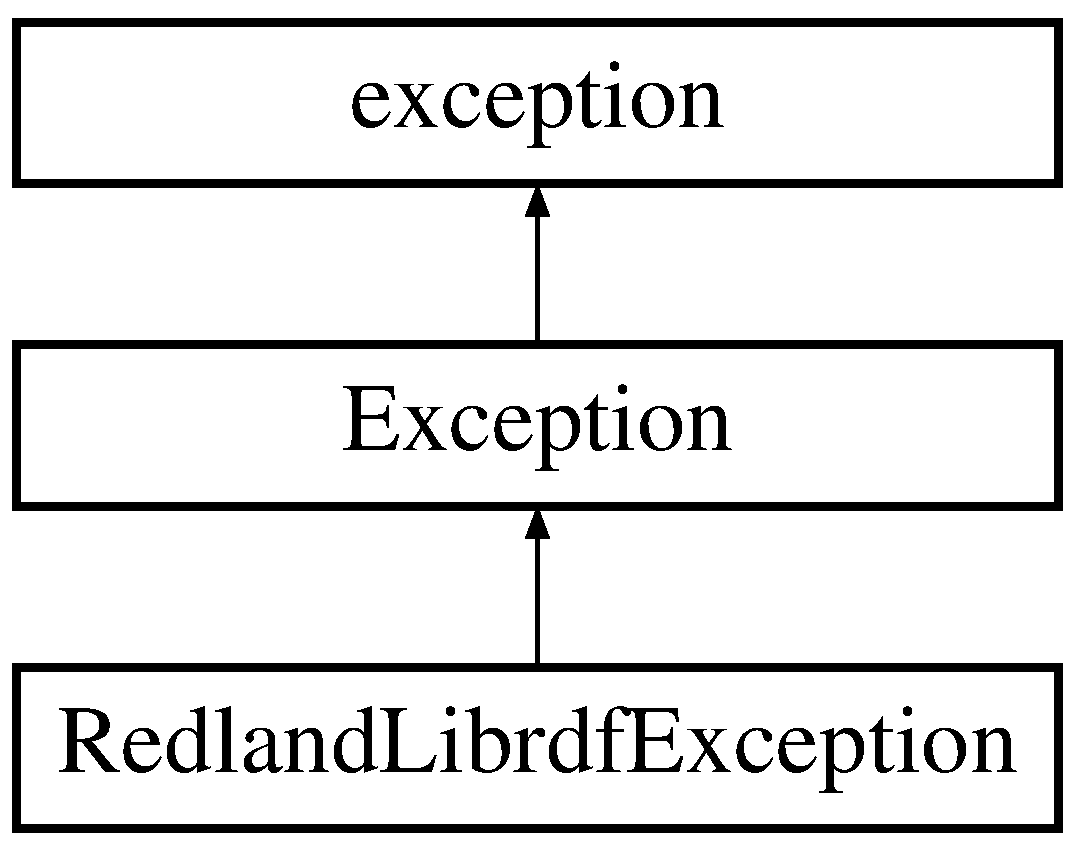
\includegraphics[height=3.000000cm]{classRedlandLibrdfException}
\end{center}
\end{figure}
\subsection*{Additional Inherited Members}


The documentation for this class was generated from the following file\+:\begin{DoxyCompactItemize}
\item 
src/redland/\+Redland\+Wrapper/src/Librdf\+Exception.\+h\end{DoxyCompactItemize}

\hypertarget{classRedlandNullPointerException}{}\section{Redland\+Null\+Pointer\+Exception Class Reference}
\label{classRedlandNullPointerException}\index{Redland\+Null\+Pointer\+Exception@{Redland\+Null\+Pointer\+Exception}}
Inheritance diagram for Redland\+Null\+Pointer\+Exception\+:\begin{figure}[H]
\begin{center}
\leavevmode
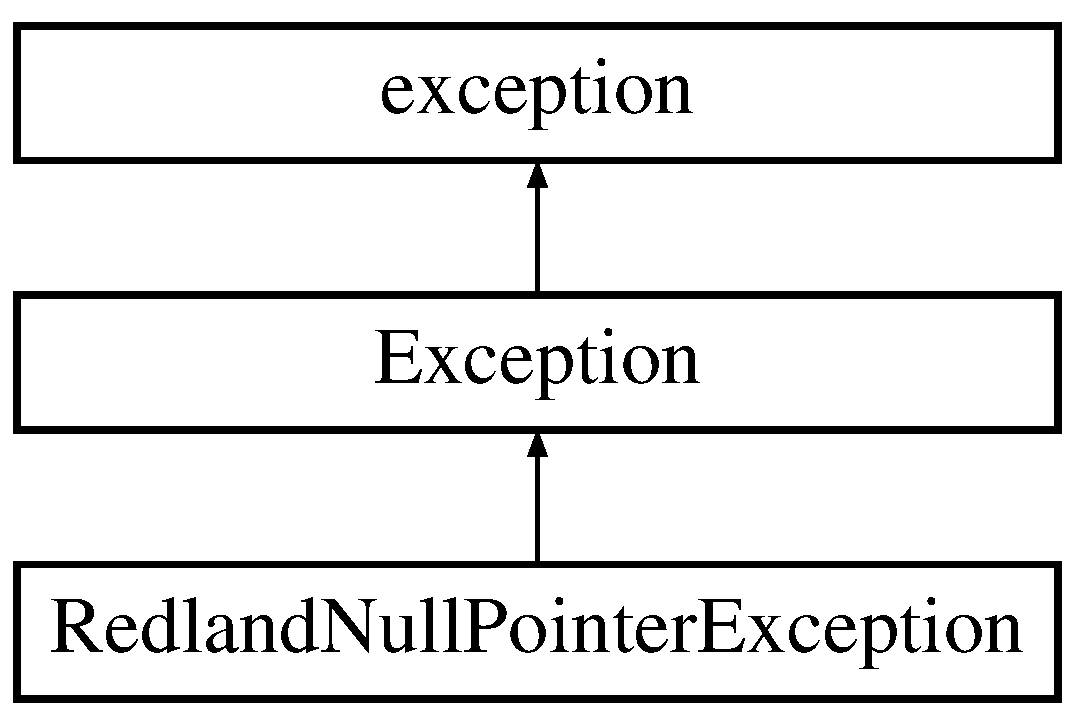
\includegraphics[height=3.000000cm]{classRedlandNullPointerException}
\end{center}
\end{figure}
\subsection*{Additional Inherited Members}


The documentation for this class was generated from the following file\+:\begin{DoxyCompactItemize}
\item 
src/redland/\+Redland\+Wrapper/src/Librdf\+Exception.\+h\end{DoxyCompactItemize}

\hypertarget{classomexmeta_1_1Resource}{}\section{omexmeta\+:\+:Resource Class Reference}
\label{classomexmeta_1_1Resource}\index{omexmeta\+::\+Resource@{omexmeta\+::\+Resource}}
\subsection*{Public Member Functions}
\begin{DoxyCompactItemize}
\item 
\mbox{\Hypertarget{classomexmeta_1_1Resource_ade5147df30b7e4f42386534a4a27b12f}\label{classomexmeta_1_1Resource_ade5147df30b7e4f42386534a4a27b12f}} 
bool {\bfseries operator==} (const \hyperlink{classomexmeta_1_1Resource}{Resource} \&rhs) const
\item 
\mbox{\Hypertarget{classomexmeta_1_1Resource_a99336c4dd6ef49588cd7144e50cf639b}\label{classomexmeta_1_1Resource_a99336c4dd6ef49588cd7144e50cf639b}} 
bool {\bfseries operator!=} (const \hyperlink{classomexmeta_1_1Resource}{Resource} \&rhs) const
\item 
\mbox{\Hypertarget{classomexmeta_1_1Resource_a6b70255d34f54c4adfa893a8ba54b0a2}\label{classomexmeta_1_1Resource_a6b70255d34f54c4adfa893a8ba54b0a2}} 
{\bfseries Resource} (\hyperlink{classredland_1_1LibrdfNode}{Librdf\+Node} node)
\item 
\mbox{\Hypertarget{classomexmeta_1_1Resource_a25be1a34d6a27565612a9c7b597befd8}\label{classomexmeta_1_1Resource_a25be1a34d6a27565612a9c7b597befd8}} 
void {\bfseries set\+Node} (librdf\+\_\+node $\ast$node)
\item 
\mbox{\Hypertarget{classomexmeta_1_1Resource_a7866b5bd47b319e39dec70eae8969d4f}\label{classomexmeta_1_1Resource_a7866b5bd47b319e39dec70eae8969d4f}} 
librdf\+\_\+node $\ast$ {\bfseries get\+Node} () const
\item 
\mbox{\Hypertarget{classomexmeta_1_1Resource_aae0948ff89d537133fd5e99bb88aa96a}\label{classomexmeta_1_1Resource_aae0948ff89d537133fd5e99bb88aa96a}} 
std\+::string {\bfseries str} () const
\item 
\mbox{\Hypertarget{classomexmeta_1_1Resource_ad6a1a5009a2b8fdacf0f53899986735a}\label{classomexmeta_1_1Resource_ad6a1a5009a2b8fdacf0f53899986735a}} 
virtual bool {\bfseries is\+Set} () const
\item 
\mbox{\Hypertarget{classomexmeta_1_1Resource_a87a7540d96d762dbd3f0b5160e575803}\label{classomexmeta_1_1Resource_a87a7540d96d762dbd3f0b5160e575803}} 
void {\bfseries free} ()
\end{DoxyCompactItemize}
\subsection*{Static Public Member Functions}
\begin{DoxyCompactItemize}
\item 
\mbox{\Hypertarget{classomexmeta_1_1Resource_a4b8f2429e43312eab63b5135fd508986}\label{classomexmeta_1_1Resource_a4b8f2429e43312eab63b5135fd508986}} 
static \hyperlink{classomexmeta_1_1Resource}{Resource} {\bfseries from\+Raw\+Ptr} (librdf\+\_\+node $\ast$node)
\end{DoxyCompactItemize}
\subsection*{Protected Attributes}
\begin{DoxyCompactItemize}
\item 
\mbox{\Hypertarget{classomexmeta_1_1Resource_a9695da843dd795e090f8b89886d432b9}\label{classomexmeta_1_1Resource_a9695da843dd795e090f8b89886d432b9}} 
librdf\+\_\+node $\ast$ {\bfseries node\+\_\+} = nullptr
\end{DoxyCompactItemize}


The documentation for this class was generated from the following files\+:\begin{DoxyCompactItemize}
\item 
src/omexmeta/Resource.\+h\item 
src/omexmeta/Resource.\+cpp\end{DoxyCompactItemize}

\hypertarget{classomexmeta_1_1SBMLAssistant}{}\section{omexmeta\+:\+:S\+B\+M\+L\+Assistant Class Reference}
\label{classomexmeta_1_1SBMLAssistant}\index{omexmeta\+::\+S\+B\+M\+L\+Assistant@{omexmeta\+::\+S\+B\+M\+L\+Assistant}}
Inheritance diagram for omexmeta\+:\+:S\+B\+M\+L\+Assistant\+:\begin{figure}[H]
\begin{center}
\leavevmode
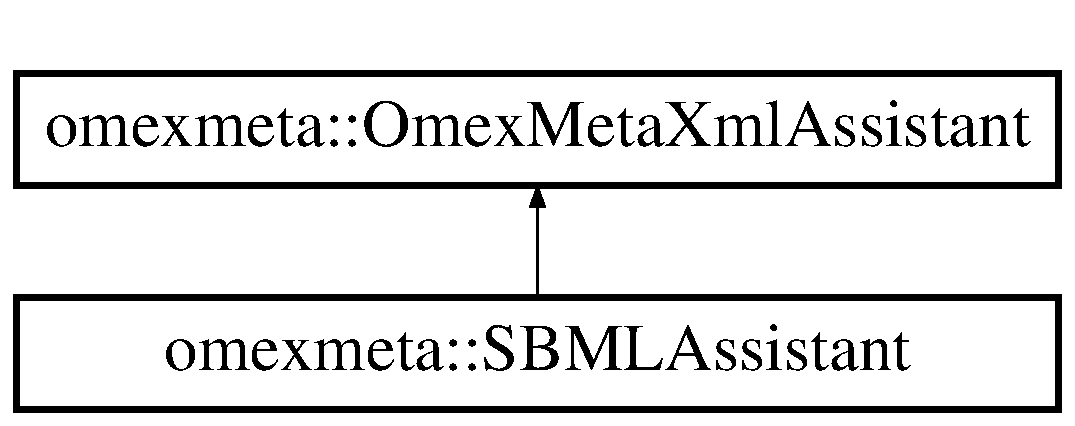
\includegraphics[height=2.000000cm]{classomexmeta_1_1SBMLAssistant}
\end{center}
\end{figure}
\subsection*{Public Member Functions}
\begin{DoxyCompactItemize}
\item 
\mbox{\Hypertarget{classomexmeta_1_1SBMLAssistant_afcc69d3e7a12673071632f757290d798}\label{classomexmeta_1_1SBMLAssistant_afcc69d3e7a12673071632f757290d798}} 
std\+::vector$<$ std\+::string $>$ {\bfseries get\+Valid\+Elements} () const override
\item 
\mbox{\Hypertarget{classomexmeta_1_1SBMLAssistant_ad3c3ab0ac3004961e5c2951568528d8a}\label{classomexmeta_1_1SBMLAssistant_ad3c3ab0ac3004961e5c2951568528d8a}} 
std\+::string {\bfseries meta\+Id\+Tag\+Name} () const override
\end{DoxyCompactItemize}


The documentation for this class was generated from the following files\+:\begin{DoxyCompactItemize}
\item 
src/omexmeta/Omex\+Meta\+Xml\+Assistant.\+h\item 
src/omexmeta/Omex\+Meta\+Xml\+Assistant.\+cpp\end{DoxyCompactItemize}

\hypertarget{classomexmeta_1_1SBMLSemanticExtraction}{}\section{omexmeta\+:\+:S\+B\+M\+L\+Semantic\+Extraction Class Reference}
\label{classomexmeta_1_1SBMLSemanticExtraction}\index{omexmeta\+::\+S\+B\+M\+L\+Semantic\+Extraction@{omexmeta\+::\+S\+B\+M\+L\+Semantic\+Extraction}}
\subsection*{Public Member Functions}
\begin{DoxyCompactItemize}
\item 
\mbox{\Hypertarget{classomexmeta_1_1SBMLSemanticExtraction_a3c55dab129bd47c753f19317fade1f18}\label{classomexmeta_1_1SBMLSemanticExtraction_a3c55dab129bd47c753f19317fade1f18}} 
{\bfseries S\+B\+M\+L\+Semantic\+Extraction} (\hyperlink{classomexmeta_1_1Editor}{Editor} $\ast$editor)
\item 
\mbox{\Hypertarget{classomexmeta_1_1SBMLSemanticExtraction_a53cda7f108b954af7fb1159773e44522}\label{classomexmeta_1_1SBMLSemanticExtraction_a53cda7f108b954af7fb1159773e44522}} 
void {\bfseries extract\+Species\+Compartment\+Semantics} ()
\item 
\mbox{\Hypertarget{classomexmeta_1_1SBMLSemanticExtraction_a89ed78df066e71e628c8b631175a8441}\label{classomexmeta_1_1SBMLSemanticExtraction_a89ed78df066e71e628c8b631175a8441}} 
void {\bfseries extract\+Processes\+From\+Reactions} ()
\end{DoxyCompactItemize}


The documentation for this class was generated from the following files\+:\begin{DoxyCompactItemize}
\item 
src/omexmeta/S\+B\+M\+L\+Semantic\+Extraction.\+h\item 
src/omexmeta/S\+B\+M\+L\+Semantic\+Extraction.\+cpp\end{DoxyCompactItemize}

\hypertarget{classomexmeta_1_1SemSim}{}\section{omexmeta\+:\+:Sem\+Sim Class Reference}
\label{classomexmeta_1_1SemSim}\index{omexmeta\+::\+Sem\+Sim@{omexmeta\+::\+Sem\+Sim}}
Inheritance diagram for omexmeta\+:\+:Sem\+Sim\+:\begin{figure}[H]
\begin{center}
\leavevmode
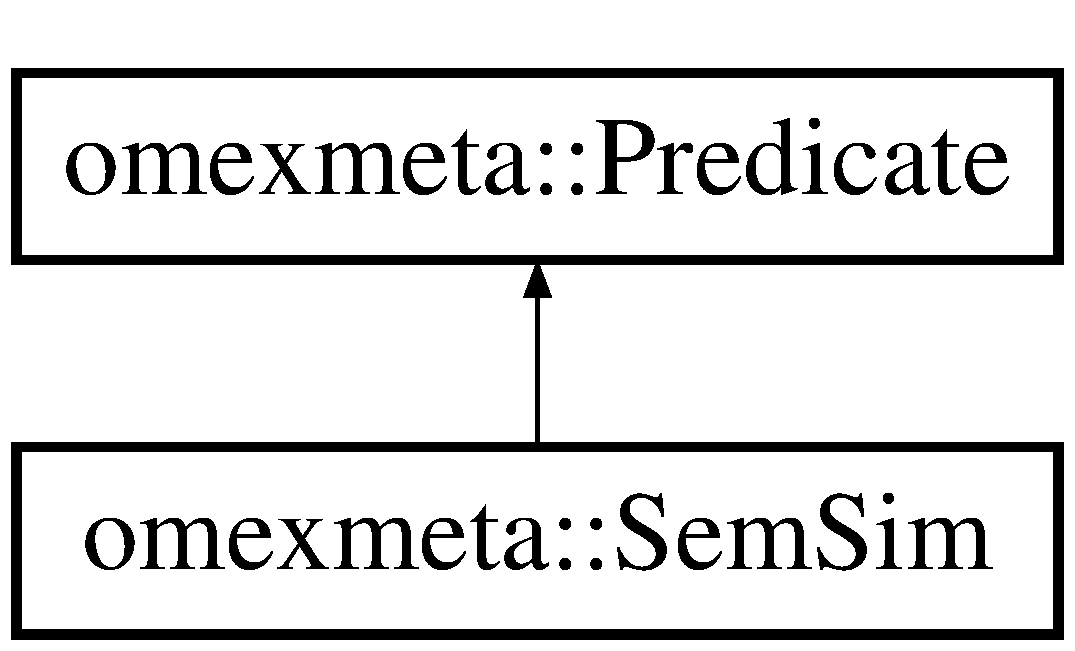
\includegraphics[height=2.000000cm]{classomexmeta_1_1SemSim}
\end{center}
\end{figure}
\subsection*{Public Member Functions}
\begin{DoxyCompactItemize}
\item 
\mbox{\Hypertarget{classomexmeta_1_1SemSim_a957a762d9f721bfc74f0db91552068a4}\label{classomexmeta_1_1SemSim_a957a762d9f721bfc74f0db91552068a4}} 
{\bfseries Sem\+Sim} (const std\+::string \&term)
\item 
\mbox{\Hypertarget{classomexmeta_1_1SemSim_a40dcb1f6945bba21cc6927cf78a53e80}\label{classomexmeta_1_1SemSim_a40dcb1f6945bba21cc6927cf78a53e80}} 
void {\bfseries verify} ()
\end{DoxyCompactItemize}
\subsection*{Public Attributes}
\begin{DoxyCompactItemize}
\item 
std\+::vector$<$ std\+::string $>$ {\bfseries valid\+\_\+terms\+\_\+}
\end{DoxyCompactItemize}
\subsection*{Additional Inherited Members}


\subsection{Member Data Documentation}
\mbox{\Hypertarget{classomexmeta_1_1SemSim_af6e027f353354892e3a26abb9b6f2ece}\label{classomexmeta_1_1SemSim_af6e027f353354892e3a26abb9b6f2ece}} 
\index{omexmeta\+::\+Sem\+Sim@{omexmeta\+::\+Sem\+Sim}!valid\+\_\+terms\+\_\+@{valid\+\_\+terms\+\_\+}}
\index{valid\+\_\+terms\+\_\+@{valid\+\_\+terms\+\_\+}!omexmeta\+::\+Sem\+Sim@{omexmeta\+::\+Sem\+Sim}}
\subsubsection{\texorpdfstring{valid\+\_\+terms\+\_\+}{valid\_terms\_}}
{\footnotesize\ttfamily std\+::vector$<$std\+::string$>$ omexmeta\+::\+Sem\+Sim\+::valid\+\_\+terms\+\_\+}

{\bfseries Initial value\+:}
\begin{DoxyCode}
\{
                \textcolor{stringliteral}{"hasSourceParticipant"},
                \textcolor{stringliteral}{"hasSinkParticipant"},
                \textcolor{stringliteral}{"hasMediatorParticipant"},
                \textcolor{stringliteral}{"hasMultiplier"},
                \textcolor{stringliteral}{"hasPhysicalEntityReference"},
        \}
\end{DoxyCode}


The documentation for this class was generated from the following files\+:\begin{DoxyCompactItemize}
\item 
src/omexmeta/Predicate.\+h\item 
src/omexmeta/Predicate.\+cpp\end{DoxyCompactItemize}

\hypertarget{classomexmeta_1_1SemsimXmlAssistantFactory}{}\section{omexmeta\+:\+:Semsim\+Xml\+Assistant\+Factory Class Reference}
\label{classomexmeta_1_1SemsimXmlAssistantFactory}\index{omexmeta\+::\+Semsim\+Xml\+Assistant\+Factory@{omexmeta\+::\+Semsim\+Xml\+Assistant\+Factory}}
\subsection*{Static Public Member Functions}
\begin{DoxyCompactItemize}
\item 
\mbox{\Hypertarget{classomexmeta_1_1SemsimXmlAssistantFactory_acd1e70258ce2a70ff459f9ff905c2371}\label{classomexmeta_1_1SemsimXmlAssistantFactory_acd1e70258ce2a70ff459f9ff905c2371}} 
static Xml\+Assistant\+Ptr {\bfseries generate} (const std\+::string \&xml, Omex\+Meta\+Xml\+Type type, bool generate\+\_\+new\+\_\+metaids=false, std\+::string metaid\+\_\+base=\char`\"{}\#Omex\+Meta\+Id\char`\"{}, int metaid\+\_\+num\+\_\+digits=4)
\end{DoxyCompactItemize}


The documentation for this class was generated from the following files\+:\begin{DoxyCompactItemize}
\item 
src/omexmeta/Omex\+Meta\+Xml\+Assistant.\+h\item 
src/omexmeta/Omex\+Meta\+Xml\+Assistant.\+cpp\end{DoxyCompactItemize}

\hypertarget{classomexmeta_1_1SinkParticipant}{}\section{omexmeta\+:\+:Sink\+Participant Class Reference}
\label{classomexmeta_1_1SinkParticipant}\index{omexmeta\+::\+Sink\+Participant@{omexmeta\+::\+Sink\+Participant}}
Inheritance diagram for omexmeta\+:\+:Sink\+Participant\+:\begin{figure}[H]
\begin{center}
\leavevmode
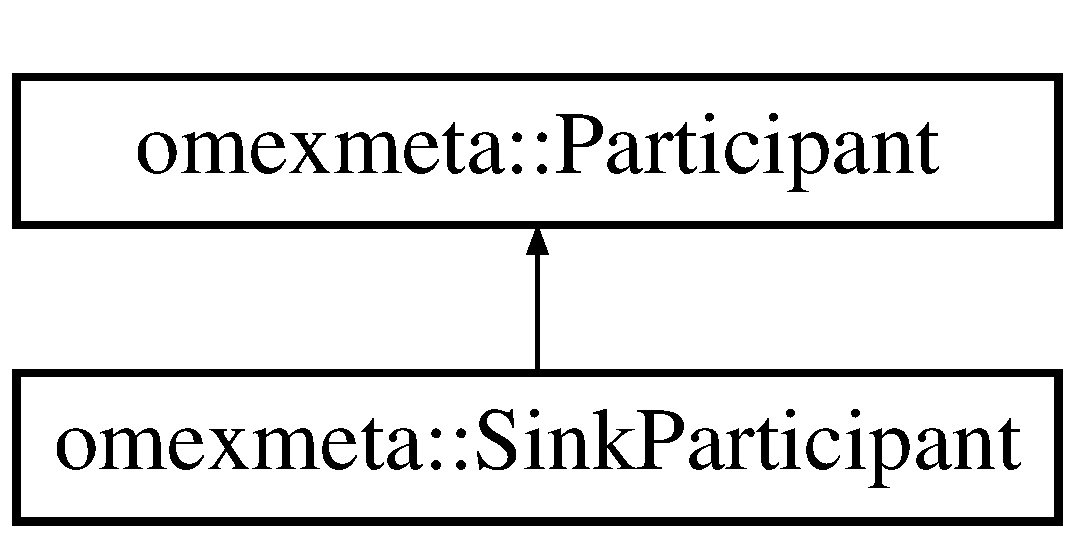
\includegraphics[height=2.000000cm]{classomexmeta_1_1SinkParticipant}
\end{center}
\end{figure}
\subsection*{Public Member Functions}
\begin{DoxyCompactItemize}
\item 
\mbox{\Hypertarget{classomexmeta_1_1SinkParticipant_a0adac71db2271549cbb6dc17346d89b7}\label{classomexmeta_1_1SinkParticipant_a0adac71db2271549cbb6dc17346d89b7}} 
{\bfseries Sink\+Participant} (librdf\+\_\+model $\ast$model, int multiplier, std\+::string physical\+Entity\+Reference, const std\+::string \&model\+\_\+uri, const std\+::string \&local\+\_\+uri)
\end{DoxyCompactItemize}


The documentation for this class was generated from the following files\+:\begin{DoxyCompactItemize}
\item 
src/omexmeta/Participant.\+h\item 
src/omexmeta/Participant.\+cpp\end{DoxyCompactItemize}

\hypertarget{classomexmeta_1_1SourceParticipant}{}\section{omexmeta\+:\+:Source\+Participant Class Reference}
\label{classomexmeta_1_1SourceParticipant}\index{omexmeta\+::\+Source\+Participant@{omexmeta\+::\+Source\+Participant}}
Inheritance diagram for omexmeta\+:\+:Source\+Participant\+:\begin{figure}[H]
\begin{center}
\leavevmode
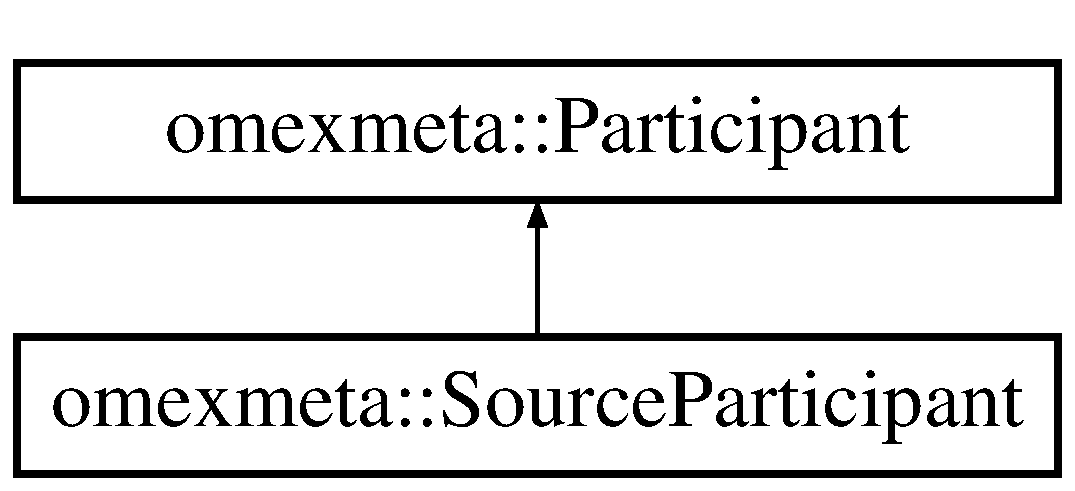
\includegraphics[height=2.000000cm]{classomexmeta_1_1SourceParticipant}
\end{center}
\end{figure}
\subsection*{Public Member Functions}
\begin{DoxyCompactItemize}
\item 
\mbox{\Hypertarget{classomexmeta_1_1SourceParticipant_a84b77b854e235cc9e0cb8da2b6a2cee5}\label{classomexmeta_1_1SourceParticipant_a84b77b854e235cc9e0cb8da2b6a2cee5}} 
{\bfseries Source\+Participant} (librdf\+\_\+model $\ast$model, int multiplier, std\+::string physical\+Entity\+Reference, const std\+::string \&model\+\_\+uri, const std\+::string \&local\+\_\+uri)
\end{DoxyCompactItemize}


The documentation for this class was generated from the following files\+:\begin{DoxyCompactItemize}
\item 
src/omexmeta/Participant.\+h\item 
src/omexmeta/Participant.\+cpp\end{DoxyCompactItemize}

\hypertarget{classomexmeta_1_1Subject}{}\section{omexmeta\+:\+:Subject Class Reference}
\label{classomexmeta_1_1Subject}\index{omexmeta\+::\+Subject@{omexmeta\+::\+Subject}}
\subsection*{Public Member Functions}
\begin{DoxyCompactItemize}
\item 
\mbox{\Hypertarget{classomexmeta_1_1Subject_a4e80ab7745a8c2cf6628e8e93a95cdac}\label{classomexmeta_1_1Subject_a4e80ab7745a8c2cf6628e8e93a95cdac}} 
{\bfseries Subject} (\hyperlink{classredland_1_1LibrdfNode}{Librdf\+Node} node)
\item 
\mbox{\Hypertarget{classomexmeta_1_1Subject_a91ea148978a5320dfba19bdb1bdbdd90}\label{classomexmeta_1_1Subject_a91ea148978a5320dfba19bdb1bdbdd90}} 
librdf\+\_\+node $\ast$ {\bfseries get\+Node} () const
\item 
\mbox{\Hypertarget{classomexmeta_1_1Subject_aa04b4e973bd7df44fffe588e31b8779f}\label{classomexmeta_1_1Subject_aa04b4e973bd7df44fffe588e31b8779f}} 
void {\bfseries set\+Node} (librdf\+\_\+node $\ast$node)
\item 
\mbox{\Hypertarget{classomexmeta_1_1Subject_a1b170dceee7bf297843da5b201e06693}\label{classomexmeta_1_1Subject_a1b170dceee7bf297843da5b201e06693}} 
bool {\bfseries operator==} (const \hyperlink{classomexmeta_1_1Subject}{Subject} \&rhs) const
\item 
\mbox{\Hypertarget{classomexmeta_1_1Subject_a3729c201061ff27fc50b1ae2412dab2b}\label{classomexmeta_1_1Subject_a3729c201061ff27fc50b1ae2412dab2b}} 
bool {\bfseries operator!=} (const \hyperlink{classomexmeta_1_1Subject}{Subject} \&rhs) const
\item 
\mbox{\Hypertarget{classomexmeta_1_1Subject_a3aa59bfd78d3c6e138beb386d846a584}\label{classomexmeta_1_1Subject_a3aa59bfd78d3c6e138beb386d846a584}} 
std\+::string {\bfseries str} () const
\item 
\mbox{\Hypertarget{classomexmeta_1_1Subject_a1b4c539f6310fc0c834cc44afb275c32}\label{classomexmeta_1_1Subject_a1b4c539f6310fc0c834cc44afb275c32}} 
bool {\bfseries is\+Set} () const
\item 
\mbox{\Hypertarget{classomexmeta_1_1Subject_ac21da4aad49780ba33322de5b7f87756}\label{classomexmeta_1_1Subject_ac21da4aad49780ba33322de5b7f87756}} 
void {\bfseries free} ()
\end{DoxyCompactItemize}
\subsection*{Static Public Member Functions}
\begin{DoxyCompactItemize}
\item 
\mbox{\Hypertarget{classomexmeta_1_1Subject_a845dda888ce07265306d0eb6b46cd989}\label{classomexmeta_1_1Subject_a845dda888ce07265306d0eb6b46cd989}} 
static \hyperlink{classomexmeta_1_1Subject}{Subject} {\bfseries from\+Raw\+Ptr} (librdf\+\_\+node $\ast$node)
\item 
\mbox{\Hypertarget{classomexmeta_1_1Subject_a346583235b81d5bd523818de09d7359e}\label{classomexmeta_1_1Subject_a346583235b81d5bd523818de09d7359e}} 
static \hyperlink{classomexmeta_1_1Subject}{Subject} {\bfseries from\+Uri} (const std\+::string \&uri)
\item 
\mbox{\Hypertarget{classomexmeta_1_1Subject_a315d058097112f4081c4db7860346aef}\label{classomexmeta_1_1Subject_a315d058097112f4081c4db7860346aef}} 
static \hyperlink{classomexmeta_1_1Subject}{Subject} {\bfseries from\+Blank} (const std\+::string \&blank)
\end{DoxyCompactItemize}


The documentation for this class was generated from the following files\+:\begin{DoxyCompactItemize}
\item 
src/omexmeta/Subject.\+h\item 
src/omexmeta/Subject.\+cpp\end{DoxyCompactItemize}

\hypertarget{structdbg_1_1time}{}\section{dbg\+:\+:time Struct Reference}
\label{structdbg_1_1time}\index{dbg\+::time@{dbg\+::time}}


The documentation for this struct was generated from the following file\+:\begin{DoxyCompactItemize}
\item 
src/omexmeta/dbg.\+h\end{DoxyCompactItemize}

\hypertarget{classomexmeta_1_1Triple}{}\section{omexmeta\+:\+:Triple Class Reference}
\label{classomexmeta_1_1Triple}\index{omexmeta\+::\+Triple@{omexmeta\+::\+Triple}}
Inheritance diagram for omexmeta\+:\+:Triple\+:\begin{figure}[H]
\begin{center}
\leavevmode
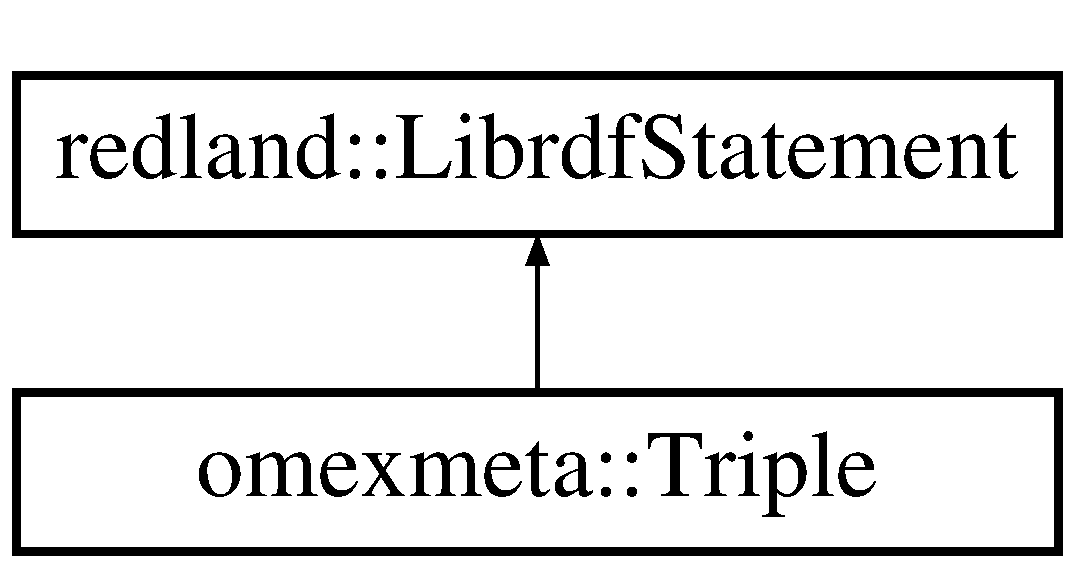
\includegraphics[height=2.000000cm]{classomexmeta_1_1Triple}
\end{center}
\end{figure}
\subsection*{Public Member Functions}
\begin{DoxyCompactItemize}
\item 
\mbox{\Hypertarget{classomexmeta_1_1Triple_aaed857f9356dc3a7414f06f393a75ba0}\label{classomexmeta_1_1Triple_aaed857f9356dc3a7414f06f393a75ba0}} 
{\bfseries Triple} (const \hyperlink{classomexmeta_1_1Subject}{Subject} \&subject, const Predicate\+Ptr \&predicate\+\_\+ptr, const \hyperlink{classomexmeta_1_1Resource}{Resource} \&resource)
\item 
\mbox{\Hypertarget{classomexmeta_1_1Triple_adc457c78ec059eb71602e7ea4f763582}\label{classomexmeta_1_1Triple_adc457c78ec059eb71602e7ea4f763582}} 
{\bfseries Triple} (librdf\+\_\+node $\ast$subject, librdf\+\_\+node $\ast$predicate, librdf\+\_\+node $\ast$resource)
\item 
\mbox{\Hypertarget{classomexmeta_1_1Triple_a1cb45dd3a5778f0e0e92e4a185da9400}\label{classomexmeta_1_1Triple_a1cb45dd3a5778f0e0e92e4a185da9400}} 
const std\+::string \& {\bfseries get\+Local\+Uri} () const
\item 
\mbox{\Hypertarget{classomexmeta_1_1Triple_a6694daa46597ea91dda045aa0d5e6cfc}\label{classomexmeta_1_1Triple_a6694daa46597ea91dda045aa0d5e6cfc}} 
void {\bfseries set\+Local\+Uri} (std\+::string local\+Uri)
\item 
\mbox{\Hypertarget{classomexmeta_1_1Triple_afd918ecccfa23079d9cb70f2e1a3e9b0}\label{classomexmeta_1_1Triple_afd918ecccfa23079d9cb70f2e1a3e9b0}} 
void {\bfseries set\+Model\+Uri} (const std\+::string \&model\+\_\+uri)
\item 
\mbox{\Hypertarget{classomexmeta_1_1Triple_aabfef726172656b6c61c602b4d8d33e5}\label{classomexmeta_1_1Triple_aabfef726172656b6c61c602b4d8d33e5}} 
std\+::string {\bfseries str} (const std\+::string \&format=\char`\"{}turtle\char`\"{}, const std\+::string \&base=(std\+::filesystem\+::current\+\_\+path()/=\char`\"{}annotations.\+rdf\char`\"{}).string(), std\+::string omex\+\_\+name=\char`\"{}New\+Omex.\+omex/\char`\"{}, std\+::string model\+\_\+name=\char`\"{}New\+Model.\+xml\#\char`\"{}) const
\item 
\mbox{\Hypertarget{classomexmeta_1_1Triple_a3f3868622349d3a3e14ed3e4b21d49a9}\label{classomexmeta_1_1Triple_a3f3868622349d3a3e14ed3e4b21d49a9}} 
void {\bfseries free\+Triple} ()
\item 
\mbox{\Hypertarget{classomexmeta_1_1Triple_a2b673a8166a19fb4feae0fc42d31c105}\label{classomexmeta_1_1Triple_a2b673a8166a19fb4feae0fc42d31c105}} 
\hyperlink{classomexmeta_1_1Triple}{Triple} \& {\bfseries set\+About} (std\+::string omex\+\_\+name, const std\+::string \&model\+\_\+name, std\+::string metaid)
\item 
\mbox{\Hypertarget{classomexmeta_1_1Triple_a6329b09efb05005d248790e8a3d507f3}\label{classomexmeta_1_1Triple_a6329b09efb05005d248790e8a3d507f3}} 
\hyperlink{classomexmeta_1_1Triple}{Triple} \& {\bfseries set\+About} (std\+::string metaid)
\item 
\mbox{\Hypertarget{classomexmeta_1_1Triple_a69df88d19e2f9077fccfa9543dadd15f}\label{classomexmeta_1_1Triple_a69df88d19e2f9077fccfa9543dadd15f}} 
std\+::string {\bfseries get\+About} () const
\item 
\mbox{\Hypertarget{classomexmeta_1_1Triple_a886240fe50becaaa47ca171f2d454ba4}\label{classomexmeta_1_1Triple_a886240fe50becaaa47ca171f2d454ba4}} 
librdf\+\_\+statement $\ast$ {\bfseries get\+Statement} () const
\item 
\mbox{\Hypertarget{classomexmeta_1_1Triple_a57b4521321178af38415e76cd483207e}\label{classomexmeta_1_1Triple_a57b4521321178af38415e76cd483207e}} 
\hyperlink{classomexmeta_1_1Triple}{Triple} \& {\bfseries set\+Predicate} (const std\+::string \&namespace\+\_\+, const std\+::string \&term)
\item 
\mbox{\Hypertarget{classomexmeta_1_1Triple_a7358812badc8d0d5589a0165af4ad375}\label{classomexmeta_1_1Triple_a7358812badc8d0d5589a0165af4ad375}} 
\hyperlink{classomexmeta_1_1Triple}{Triple} \& {\bfseries set\+Resource\+Literal} (const std\+::string \&literal)
\item 
\mbox{\Hypertarget{classomexmeta_1_1Triple_ae6836c6e9d06a310a120345aa95a4daa}\label{classomexmeta_1_1Triple_ae6836c6e9d06a310a120345aa95a4daa}} 
\hyperlink{classomexmeta_1_1Triple}{Triple} \& {\bfseries set\+Resource\+Uri} (const std\+::string \&identifiers\+\_\+uri)
\item 
\mbox{\Hypertarget{classomexmeta_1_1Triple_a90ffe9b74d354cc3fe3132a07546f6d1}\label{classomexmeta_1_1Triple_a90ffe9b74d354cc3fe3132a07546f6d1}} 
\hyperlink{classomexmeta_1_1Triple}{Triple} \& {\bfseries set\+Resource\+Blank} (const std\+::string \&blank\+\_\+id)
\item 
\mbox{\Hypertarget{classomexmeta_1_1Triple_a34832780748d58b0fddea6f6f079217a}\label{classomexmeta_1_1Triple_a34832780748d58b0fddea6f6f079217a}} 
bool {\bfseries is\+Empty} ()
\item 
\mbox{\Hypertarget{classomexmeta_1_1Triple_a1a99a566a9d1883c6329a023f4dbc056}\label{classomexmeta_1_1Triple_a1a99a566a9d1883c6329a023f4dbc056}} 
\hyperlink{classomexmeta_1_1Triple}{Triple} \& {\bfseries set\+Predicate} (const std\+::string \&uri)
\item 
\mbox{\Hypertarget{classomexmeta_1_1Triple_ab89993902b551b98d9e17e4fe5ebed6b}\label{classomexmeta_1_1Triple_ab89993902b551b98d9e17e4fe5ebed6b}} 
void {\bfseries free\+Triple\+And\+Uris} ()
\item 
\mbox{\Hypertarget{classomexmeta_1_1Triple_ac379e5410a41c1946e91d581f023c7f5}\label{classomexmeta_1_1Triple_ac379e5410a41c1946e91d581f023c7f5}} 
const std\+::string \& {\bfseries get\+Model\+Uri} () const
\item 
\mbox{\Hypertarget{classomexmeta_1_1Triple_a44d31389b0056ab4f1d8689521a25032}\label{classomexmeta_1_1Triple_a44d31389b0056ab4f1d8689521a25032}} 
\hyperlink{classomexmeta_1_1Triple}{Triple} \& {\bfseries set\+Resource\+With\+Model\+Uri} (const std\+::string \&metaid)
\end{DoxyCompactItemize}
\subsection*{Static Public Member Functions}
\begin{DoxyCompactItemize}
\item 
\mbox{\Hypertarget{classomexmeta_1_1Triple_af03c0ce3392c0ff30f13772209ac873c}\label{classomexmeta_1_1Triple_af03c0ce3392c0ff30f13772209ac873c}} 
static \hyperlink{classomexmeta_1_1Triple}{Triple} {\bfseries from\+Raw\+Statement\+Ptr} (librdf\+\_\+statement $\ast$statement)
\end{DoxyCompactItemize}
\subsection*{Additional Inherited Members}


The documentation for this class was generated from the following files\+:\begin{DoxyCompactItemize}
\item 
src/omexmeta/Triple.\+h\item 
src/omexmeta/Triple.\+cpp\end{DoxyCompactItemize}

\hypertarget{classomexmeta_1_1Triples}{}\section{omexmeta\+:\+:Triples Class Reference}
\label{classomexmeta_1_1Triples}\index{omexmeta\+::\+Triples@{omexmeta\+::\+Triples}}
\subsection*{Public Member Functions}
\begin{DoxyCompactItemize}
\item 
\mbox{\Hypertarget{classomexmeta_1_1Triples_a32ea34c1fd3bfe9887c2221377392efe}\label{classomexmeta_1_1Triples_a32ea34c1fd3bfe9887c2221377392efe}} 
{\bfseries Triples} (int size)
\item 
\mbox{\Hypertarget{classomexmeta_1_1Triples_a733eea0f6a2c206eb96771bc7a8cb430}\label{classomexmeta_1_1Triples_a733eea0f6a2c206eb96771bc7a8cb430}} 
{\bfseries Triples} (\hyperlink{classomexmeta_1_1Triple}{Triple} \&triple)
\item 
\mbox{\Hypertarget{classomexmeta_1_1Triples_a71a3ff7b185a5420eabd9bf4e9637196}\label{classomexmeta_1_1Triples_a71a3ff7b185a5420eabd9bf4e9637196}} 
{\bfseries Triples} (std\+::vector$<$ \hyperlink{classomexmeta_1_1Triple}{Triple} $>$ triples)
\item 
\mbox{\Hypertarget{classomexmeta_1_1Triples_a8c6e00fe9e694d9c52e1fa37a82ae489}\label{classomexmeta_1_1Triples_a8c6e00fe9e694d9c52e1fa37a82ae489}} 
bool {\bfseries operator==} (const \hyperlink{classomexmeta_1_1Triples}{Triples} \&rhs) const
\item 
\mbox{\Hypertarget{classomexmeta_1_1Triples_a8c9df0d37572179d682127cb7368dd82}\label{classomexmeta_1_1Triples_a8c9df0d37572179d682127cb7368dd82}} 
bool {\bfseries operator!=} (const \hyperlink{classomexmeta_1_1Triples}{Triples} \&rhs) const
\item 
\mbox{\Hypertarget{classomexmeta_1_1Triples_a88dcf4b950f105acb621bd07f07a38a0}\label{classomexmeta_1_1Triples_a88dcf4b950f105acb621bd07f07a38a0}} 
void {\bfseries move\+\_\+back} (\hyperlink{classomexmeta_1_1Triple}{Triple} \&triple)
\item 
\mbox{\Hypertarget{classomexmeta_1_1Triples_a9882f6f582e8d2e34e09d2f7076a0e2e}\label{classomexmeta_1_1Triples_a9882f6f582e8d2e34e09d2f7076a0e2e}} 
void {\bfseries emplace\+\_\+back} (\hyperlink{classomexmeta_1_1Subject}{Subject} subject, const Predicate\+Ptr \&predicate\+Ptr, const \hyperlink{classomexmeta_1_1Resource}{Resource} \&resource)
\item 
\mbox{\Hypertarget{classomexmeta_1_1Triples_acab4513889a9a42c77b3044aac941728}\label{classomexmeta_1_1Triples_acab4513889a9a42c77b3044aac941728}} 
void {\bfseries emplace\+\_\+back} (\hyperlink{classomexmeta_1_1Subject}{Subject} subject, const \hyperlink{classomexmeta_1_1Predicate}{Predicate} \&predicate, const \hyperlink{classomexmeta_1_1Resource}{Resource} \&resource)
\item 
\mbox{\Hypertarget{classomexmeta_1_1Triples_a862d672c0ac9d877261947cf5a7061db}\label{classomexmeta_1_1Triples_a862d672c0ac9d877261947cf5a7061db}} 
void {\bfseries emplace\+\_\+back} (\hyperlink{classomexmeta_1_1Subject}{Subject} subject, \hyperlink{classomexmeta_1_1BiomodelsBiologyQualifier}{Biomodels\+Biology\+Qualifier} predicate, const \hyperlink{classomexmeta_1_1Resource}{Resource} \&resource)
\item 
\mbox{\Hypertarget{classomexmeta_1_1Triples_a87cdc3aacef07c2aebbfe06342bd70f5}\label{classomexmeta_1_1Triples_a87cdc3aacef07c2aebbfe06342bd70f5}} 
void {\bfseries emplace\+\_\+back} (\hyperlink{classomexmeta_1_1Subject}{Subject} subject, \hyperlink{classomexmeta_1_1BiomodelsModelQualifier}{Biomodels\+Model\+Qualifier} predicate, const \hyperlink{classomexmeta_1_1Resource}{Resource} \&resource)
\item 
\mbox{\Hypertarget{classomexmeta_1_1Triples_a9f3f3152592f99ac95f65e0e7ce3b450}\label{classomexmeta_1_1Triples_a9f3f3152592f99ac95f65e0e7ce3b450}} 
void {\bfseries emplace\+\_\+back} (\hyperlink{classomexmeta_1_1Subject}{Subject} subject, \hyperlink{classomexmeta_1_1DCTerm}{D\+C\+Term} predicate, const \hyperlink{classomexmeta_1_1Resource}{Resource} \&resource)
\item 
\mbox{\Hypertarget{classomexmeta_1_1Triples_a55e7ed1c3212ae19d2189a386b81422e}\label{classomexmeta_1_1Triples_a55e7ed1c3212ae19d2189a386b81422e}} 
void {\bfseries emplace\+\_\+back} (\hyperlink{classomexmeta_1_1Subject}{Subject} subject, \hyperlink{classomexmeta_1_1SemSim}{Sem\+Sim} predicate, const \hyperlink{classomexmeta_1_1Resource}{Resource} \&resource)
\item 
\mbox{\Hypertarget{classomexmeta_1_1Triples_a3a8c150cff4d1e78aa360d62d3d6604e}\label{classomexmeta_1_1Triples_a3a8c150cff4d1e78aa360d62d3d6604e}} 
void {\bfseries emplace\+\_\+back} (librdf\+\_\+node $\ast$subject, librdf\+\_\+node $\ast$predicate, librdf\+\_\+node $\ast$resource)
\item 
\mbox{\Hypertarget{classomexmeta_1_1Triples_a5234882414a2aaaca603eacd805df3d6}\label{classomexmeta_1_1Triples_a5234882414a2aaaca603eacd805df3d6}} 
std\+::vector$<$ std\+::string $>$ {\bfseries get\+Subjects\+Str} ()
\item 
\mbox{\Hypertarget{classomexmeta_1_1Triples_a63639c08caac19e6c5cbf30bb28292d0}\label{classomexmeta_1_1Triples_a63639c08caac19e6c5cbf30bb28292d0}} 
std\+::vector$<$ std\+::string $>$ {\bfseries get\+Predicates} ()
\item 
\mbox{\Hypertarget{classomexmeta_1_1Triples_aa875120a73cb1618be9e699e8bfb08c4}\label{classomexmeta_1_1Triples_aa875120a73cb1618be9e699e8bfb08c4}} 
std\+::vector$<$ std\+::string $>$ {\bfseries get\+Resources} ()
\item 
\mbox{\Hypertarget{classomexmeta_1_1Triples_adc86427b3563d04849336a8da7566451}\label{classomexmeta_1_1Triples_adc86427b3563d04849336a8da7566451}} 
int {\bfseries size} () const
\item 
\mbox{\Hypertarget{classomexmeta_1_1Triples_aa6735eb506ff0d5a3179fab3af3b2602}\label{classomexmeta_1_1Triples_aa6735eb506ff0d5a3179fab3af3b2602}} 
Triple\+Vector\+::iterator {\bfseries begin} ()
\item 
\mbox{\Hypertarget{classomexmeta_1_1Triples_a4312337b242280bcb119908c0334bfd8}\label{classomexmeta_1_1Triples_a4312337b242280bcb119908c0334bfd8}} 
Triple\+Vector\+::iterator {\bfseries end} ()
\item 
\mbox{\Hypertarget{classomexmeta_1_1Triples_ad2510c5b335b0266b05507c53bcc64af}\label{classomexmeta_1_1Triples_ad2510c5b335b0266b05507c53bcc64af}} 
std\+::string {\bfseries str} (const std\+::string \&format=\char`\"{}turtle\char`\"{}, std\+::string base=(std\+::filesystem\+::current\+\_\+path()/=\char`\"{}annotations.\+rdf\char`\"{}).string(), std\+::string omex\+\_\+name=\char`\"{}New\+Omex.\+omex/\char`\"{}, std\+::string model\+\_\+name=\char`\"{}New\+Model.\+xml\#\char`\"{})
\item 
\mbox{\Hypertarget{classomexmeta_1_1Triples_ad0c5839b0f49d6427cf53004baf9b0f4}\label{classomexmeta_1_1Triples_ad0c5839b0f49d6427cf53004baf9b0f4}} 
void {\bfseries free\+Triples} ()
\item 
\mbox{\Hypertarget{classomexmeta_1_1Triples_a5dad8f2cde0a3f6c0ce341338f80b0cd}\label{classomexmeta_1_1Triples_a5dad8f2cde0a3f6c0ce341338f80b0cd}} 
\hyperlink{classomexmeta_1_1Triple}{Triple} {\bfseries pop} ()
\item 
\mbox{\Hypertarget{classomexmeta_1_1Triples_a43d540423a436986d9f72d7cf0f02d72}\label{classomexmeta_1_1Triples_a43d540423a436986d9f72d7cf0f02d72}} 
const \hyperlink{classomexmeta_1_1Triple}{Triple} \& {\bfseries operator\mbox{[}$\,$\mbox{]}} (int index) const
\item 
\mbox{\Hypertarget{classomexmeta_1_1Triples_a48ab93d0e38e3cfcb4eac9264b047f0a}\label{classomexmeta_1_1Triples_a48ab93d0e38e3cfcb4eac9264b047f0a}} 
bool {\bfseries is\+Empty} ()
\item 
\mbox{\Hypertarget{classomexmeta_1_1Triples_abb333b83c7a8ed1f210816ef88c8d3a0}\label{classomexmeta_1_1Triples_abb333b83c7a8ed1f210816ef88c8d3a0}} 
\hyperlink{classomexmeta_1_1Triple}{Triple} {\bfseries pop\+\_\+front} ()
\item 
\mbox{\Hypertarget{classomexmeta_1_1Triples_a1f7ba9d5cd575ba5c63ed9dbbd1f279c}\label{classomexmeta_1_1Triples_a1f7ba9d5cd575ba5c63ed9dbbd1f279c}} 
int {\bfseries capacity} ()
\end{DoxyCompactItemize}


The documentation for this class was generated from the following files\+:\begin{DoxyCompactItemize}
\item 
src/omexmeta/Triples.\+h\item 
src/omexmeta/Triples.\+cpp\end{DoxyCompactItemize}

\hypertarget{structdbg_1_1type__tag}{}\section{dbg\+:\+:type\+\_\+tag$<$ T $>$ Struct Template Reference}
\label{structdbg_1_1type__tag}\index{dbg\+::type\+\_\+tag$<$ T $>$@{dbg\+::type\+\_\+tag$<$ T $>$}}


The documentation for this struct was generated from the following file\+:\begin{DoxyCompactItemize}
\item 
src/omexmeta/dbg.\+h\end{DoxyCompactItemize}

\hypertarget{classomexmeta_1_1ValueException}{}\section{omexmeta\+:\+:Value\+Exception Class Reference}
\label{classomexmeta_1_1ValueException}\index{omexmeta\+::\+Value\+Exception@{omexmeta\+::\+Value\+Exception}}
Inheritance diagram for omexmeta\+:\+:Value\+Exception\+:\begin{figure}[H]
\begin{center}
\leavevmode
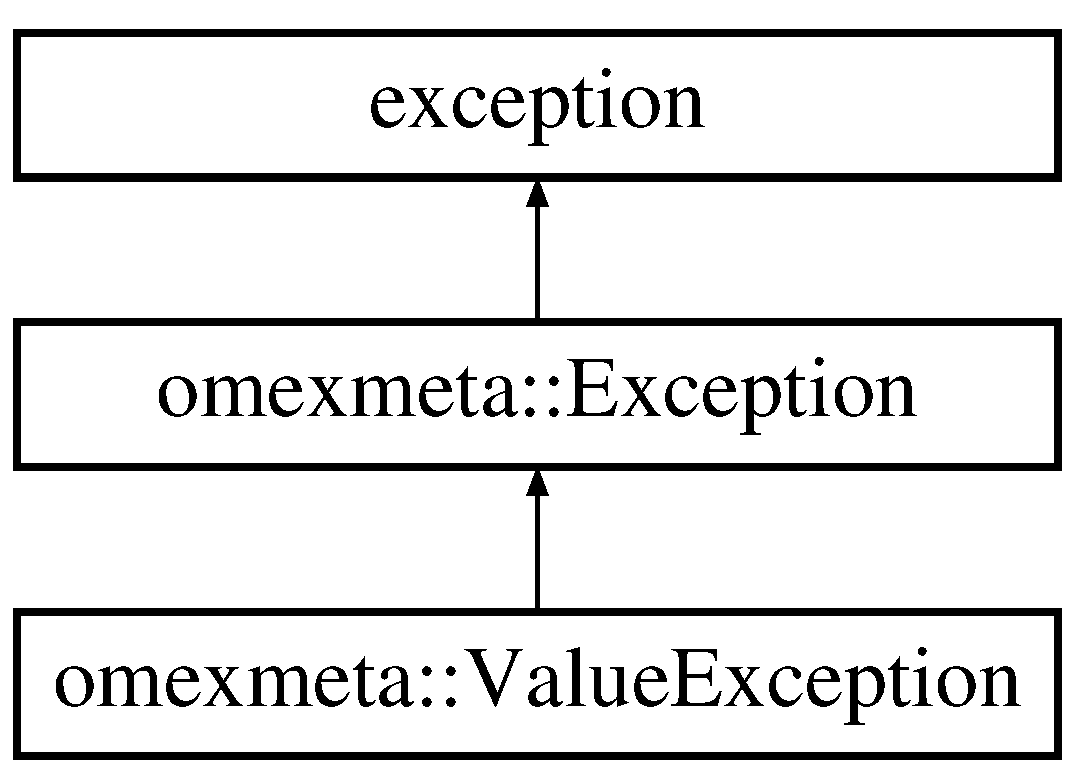
\includegraphics[height=3.000000cm]{classomexmeta_1_1ValueException}
\end{center}
\end{figure}
\subsection*{Additional Inherited Members}


The documentation for this class was generated from the following file\+:\begin{DoxyCompactItemize}
\item 
src/omexmeta/Error.\+h\end{DoxyCompactItemize}

\hypertarget{classredland_1_1World}{}\section{redland\+:\+:World Class Reference}
\label{classredland_1_1World}\index{redland\+::\+World@{redland\+::\+World}}
\subsection*{Static Public Member Functions}
\begin{DoxyCompactItemize}
\item 
\mbox{\Hypertarget{classredland_1_1World_ad7618363c9b7da4c87367707c1a159d7}\label{classredland_1_1World_ad7618363c9b7da4c87367707c1a159d7}} 
static librdf\+\_\+world $\ast$ {\bfseries get\+World} ()
\item 
\mbox{\Hypertarget{classredland_1_1World_aac0ce4018279ced7b38a36d74bb10cec}\label{classredland_1_1World_aac0ce4018279ced7b38a36d74bb10cec}} 
static raptor\+\_\+world $\ast$ {\bfseries get\+Raptor} ()
\item 
\mbox{\Hypertarget{classredland_1_1World_ade64918f10ee6ee0f5b8a0cb2e01666b}\label{classredland_1_1World_ade64918f10ee6ee0f5b8a0cb2e01666b}} 
static void {\bfseries free} (librdf\+\_\+world $\ast$world)
\end{DoxyCompactItemize}


The documentation for this class was generated from the following files\+:\begin{DoxyCompactItemize}
\item 
src/redland/\+Redland\+Wrapper/src/World.\+h\item 
src/redland/\+Redland\+Wrapper/src/World.\+cpp\end{DoxyCompactItemize}

%--- End generated contents ---

% Index
\backmatter
\newpage
\phantomsection
\clearemptydoublepage
\addcontentsline{toc}{chapter}{Index}
\printindex

\end{document}
